\documentclass[preprint,onecolumn,9pt]{sigplanconf} %{onecol}
\usepackage{alltt,mathpartir}
\usepackage{amsmath,amsthm}
\usepackage{amssymb}
\usepackage{stmaryrd}
\usepackage{url}
\usepackage{graphicx}
\usepackage{balance}
\usepackage{calc}

\newtheorem{theorem}{Theorem}
\newtheorem{lemma}{Lemma}

\newcommand{\naive}{naive}
\newcommand{\naively}{naively}
\newcommand{\Naive}{Naive}
\newcommand{\Naively}{Naively}
% \usepackage{xltxtra}
% \setmonofont[Scale=MatchLowercase]{DejaVu Sans Mono}
%
\newcommand{\superscript}[1]{\ensuremath{^{#1}}}
\newcommand{\subscript}[1]{\ensuremath{_{#1}}}
\newcommand{\tuple}[3][\ ]{{\tt #2{#1}}({#3})}

% Values
\newcommand{\clos}[1]{\tuple{clos}{#1}}
\newcommand{\rlos}[1]{\tuple{rlos}{#1}}

% States
\newcommand{\ev}[2][\ ]{\tuple[#1]{ev}{#2}}
\newcommand{\co}[1]{\tuple{co}{#1}}
\newcommand{\ap}[2][\ ]{\tuple[#1]{ap}{#2}}
\newcommand{\ans}[1]{\tuple{ans}{#1}}

% Continuations
\newcommand{\kmt}{\tt mt}
\newcommand{\kar}[2][\ ]{\tuple[#1]{ar}{#2}}
\newcommand{\kfn}[2][\ ]{\tuple[#1]{fn}{#2}}
\newcommand{\kif}[2][\ ]{\tuple[#1]{fi}{#2}}
\newcommand{\kuop}[2][\ ]{\tuple[#1]{oa}{#2}}
\newcommand{\kbopa}[2][\ ]{\tuple[#1]{oa1}{#2}}
\newcommand{\kbopb}[2][\ ]{\tuple[#1]{oa2}{#2}}

% Implementation forms
\newcommand{\generator}{{\tt generator}}
\newcommand{\yield}[1]{{\tt yield} #1}

% Syntax
\newcommand{\syntax}[1]{{\tt #1}}
\newcommand{\sapp}[3][\ ]{\tuple[#1]{app}{#2,#3}}
\newcommand{\slam}[3][\ ]{\tuple[#1]{lam}{#2,#3}}
\newcommand{\srec}[4][\ ]{\tuple[#1]{rec}{#2,#3,#4}}
\newcommand{\svar}[2][\ ]{\tuple[#1]{var}{#2}}
\newcommand{\snum}[2][\ ]{\tuple[#1]{num}{#2}}
\newcommand{\sbln}[2][\ ]{\tuple[#1]{bool}{#2}}
\newcommand{\sif}[4][\ ]{\tuple[#1]{if}{#2,#3,#4}}
\newcommand{\sop}[2][\ ]{\tuple[#1]{op}{#2}}
\newcommand{\sopu}[3][\ ]{\tuple[#1]{op}{#2,#3}}
\newcommand{\sopb}[4][\ ]{\tuple[#1]{op2}{#2,#3,#4}}
\newcommand{\strue}{{\tt tt}}
\newcommand{\sfalse}{{\tt ff}}
\newcommand{\saddone}{{\tt add1}}
\newcommand{\ssubone}{{\tt sub1}}
\newcommand{\szerohuh}{\syntax{zero?}}
\newcommand{\szero}{\syntax{0}}
\newcommand{\slit}[2][\ ]{\tuple[#1]{lit}{#2}}

\newcommand{\sNum}{\syntax{Z}}

% Metavariables
\newcommand{\maddr}{a}
\newcommand{\mvar}{x}
\newcommand{\mvarf}{f}
\newcommand{\mexp}{e}
\newcommand{\mexpi}[1]{e_{#1}}
\newcommand{\mexpf}{f}
\newcommand{\menv}{\rho}
\newcommand{\mkont}{\kappa}
\newcommand{\msto}{\sigma}
\newcommand{\mop}{o}
\newcommand{\mval}{v}
\newcommand{\mnum}{z}
\newcommand{\mbln}{b}
\newcommand{\mvalx}[1]{#1}
\newcommand\machstep{\longmapsto}
\newcommand\multimachstep{\longmapsto\!\!\!\!\!\rightarrow}
\newcommand{\mlit}{l}
\newcommand{\mstate}{\varsigma}
\newcommand{\mcomp}{k}
\newcommand{\mcompi}[1]{\mcomp_{#1}}
\newcommand{\interpdelta}{\Delta}

\newcommand{\compile}[1]{\llbracket#1\rrbracket}

\newcommand{\mlab}{{\ell}}
\newcommand{\mcntr}{{\delta}}
\newcommand{\mtcntr}{{\epsilon}}


\begin{document}

\conferenceinfo{WXYZ '05}{date, City.}
\copyrightyear{2005}
\copyrightdata{[to be supplied]}

% \titlebanner{banner above paper title}        % These are ignored unless
% \preprintfooter{short description of paper}   % 'preprint' option specified.

\title{Provably Correct, Low-Cost Optimizations for Abstract Abstract Machines}

\authorinfo{J. Ian Johnson}
           {Northeastern University}
           {ianj@ccs.neu.edu}
\authorinfo{Nicholas Labich}
           {Northeastern University}
           {labichn@ccs.neu.edu}
\authorinfo{Matthew Might}
           {University of Utah}
           {might@cs.utah.edu}
\authorinfo{David Van Horn}
           {Northeastern University}
           {dvanhorn@ccs.neu.edu}
\maketitle

\begin{abstract}
Abstracting abstract machines has been proposed as a
lightweight approach to designing sound and computable program
analyses.  The approach derives abstract interpreters from
existing machine semantics and has been applied to a variety of
languages with features widely considered difficult to analyze.
Although sound analyzers are straightforward to build under this approach,
they are also prohibitively inefficient.

This article contributes a step-by-step process for going from a
\naive{} analyzer derived under the abstracting abstract machine
approach to an efficient program analyzer.  The end result of the
process is a two to three order-of-magnitude improvement over the
systematically derived analyzer, making it competitive with
hand-optimized implementations that compute fundamentally less precise
results.
\end{abstract}

%% \category{CR-number}{subcategory}{third-level}

%% \terms
%% term1, term2

%% \keywords
%% keyword1, keyword2

\section{Introduction}

The \emph{abstracting abstract machines} (AAM)
approach~\cite{dvanhorn:VanHorn2011Abstracting,dvanhorn:VanHorn2012Systematic}
to deriving program analyses provides a systematic way of transforming a
programming language semantics in the form of an abstract machine into a family
of abstract interpreters.
%
The approach parameterizes these families with policies for regulating analytic
precision.
%
While flexible and robust, the AAM approach unfortunately yields analyzers with
poor performance relative to hand-optimized analyzers.
%
Our work takes aim squarely at this ``efficiency gap,'' and narrows it in an
equally systematic way.

%
% Specifically, these policies tune precision for control,
% the environment, the store, and base value domains.  

By taking a
machine-oriented view of computation, AAM makes it possible to design,
verify, and implement program analyzers for realistic language
features typically considered difficult to model.  The approach was
originally applied to features such as higher-order functions,
stack inspection, exceptions, laziness, first-class continuations, and
garbage collection.  It has since been used to verify actor-
\cite{local:DOsualdo:12A} and
thread-based~\cite{dvanhorn:Might2011Family} parallelism and
behavioral contracts~\cite{dvanhorn:TobinHochstadt2012Higherorder}; it
has been used to model Coq~\cite{local:harvard},
Dalvik~\cite{local:dalvik}, Erlang~\cite{local:DOsualdo:12B},
JavaScript~\cite{local:DBLP:journals/corr/abs-1109-4467}, and
Racket~\cite{dvanhorn:TobinHochstadt2012Higherorder}.

The primary strength of the approach is that abstract interpreters can
be easily derived through a small number of steps from existing
machine models.  Since the relationships between abstract machines and
higher-level semantic models---such as definitional
interpreters~\cite{dvanhorn:reynolds-hosc98}, structured operational
semantics~\cite{dvanhorn:Plotkin1981Structural}, and reduction
semantics~\cite{dvanhorn:Felleisen2009Semantics}---are well
understood~\cite{dvanhorn:Danvy:DSc}, it is possible to navigate from
these high-level semantic models to sound program analyzers in a
systematic way.  Moreover, since these analyses so closely resemble a
language's interpreter (a) implementing an analysis requires little
more than implementing an interpreter, (b) a single implementation can
serve as both an interpreter and analyzer, and (c) verifying the
correctness of the implementation is straightforward.

However, there is a considerable weakness to the approach: an
analyzer designed and implemented by following the AAM recipe is
prohibitively inefficient without both further approximation and
further implementation effort.

In this article, we develop a systematic approach to deriving a
practical implementation of an abstract-machine-based analyzer using
mostly semantic means - not tricky engineering. Our goal is to empower
programming language implementers and researchers to explore and
convincingly exhibit their ideas with a low barrier to entry. The
optimizations we describe are widely applicable and apparently
effective to scale far beyond toy examples.

\section{At a glance}

\begin{figure}[t]
\begin{center}
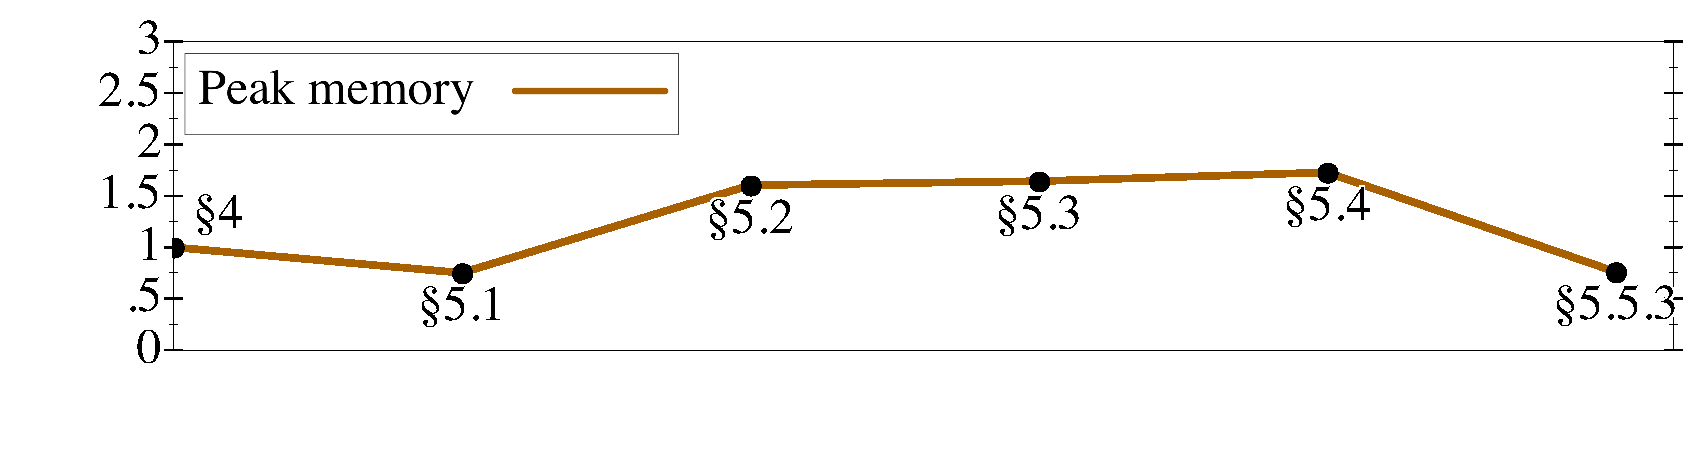
\includegraphics[width=3.2in]{church-relative-space}
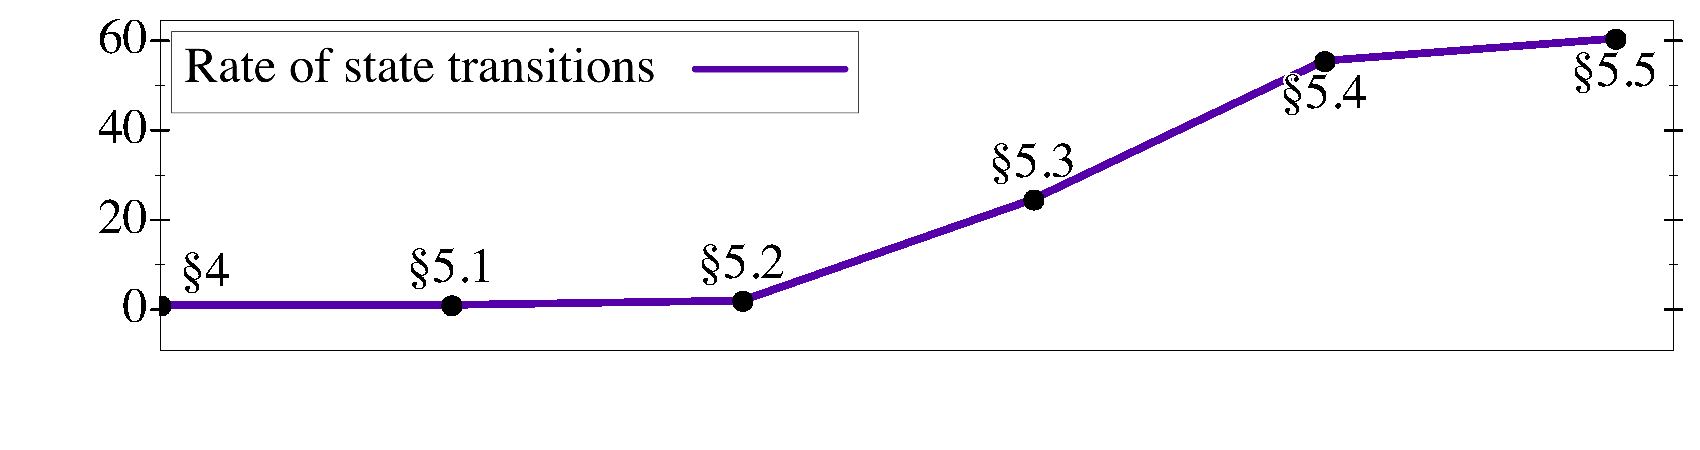
\includegraphics[width=3.2in]{church-relative-speed}
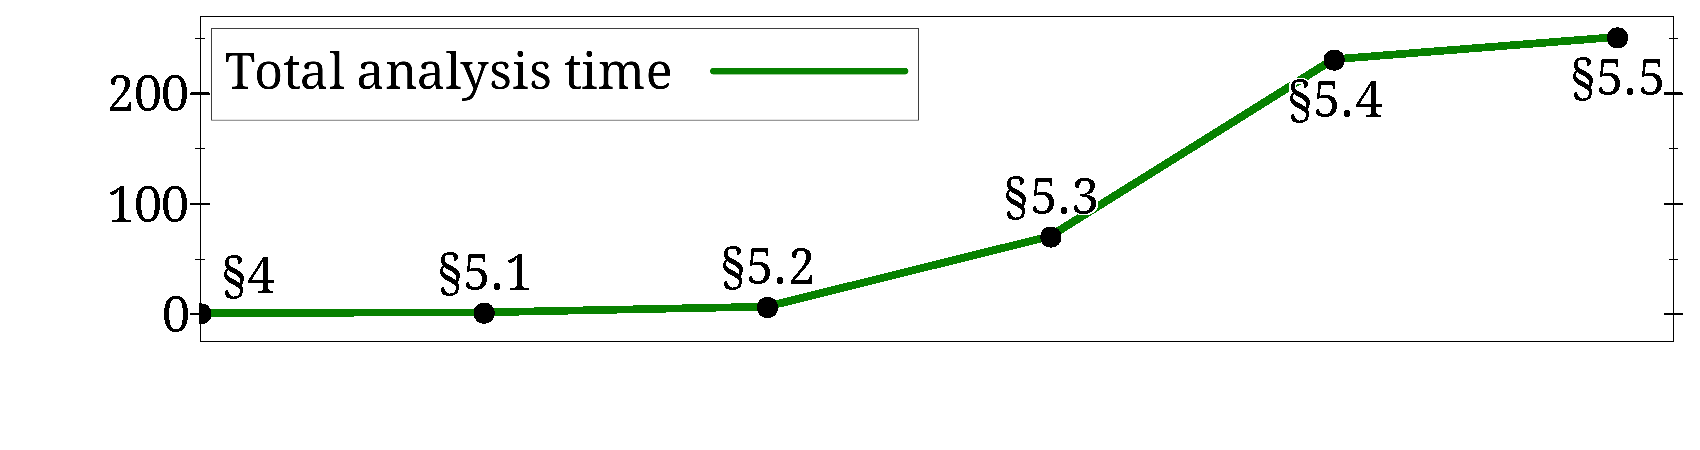
\includegraphics[width=3.2in]{church-relative-time}
\vspace{-1.5em}
\end{center}
\caption{Factor improvements over the baseline analyzer for the
  \Church{} benchmark in terms of peak memory usage, the rate of state
  transitions, and total analysis time. (Bigger is better.) Each point
  is marked with the section that introduces the optimization.}
\label{fig:churchtime}
\end{figure}


We start with a quick review of the AAM approach to develop an
analysis framework and then apply our step-by-step optimization
techniques in the simplified setting of a core functional language.
This allows us to explicate the optimizations with a minimal amount of
inessential technical overhead.  Following that, we scale this
approach up to an analyzer for a realistic untyped, higher-order
imperative language with a number of interesting features and then
measure improvements across a suite of benchmarks.

At each step during the initial presentation and development, we
evaluated the implementation on a set of benchmarks. The highlighted
benchmark in figure \ref{fig:churchtime} is from Vardoulakis and
Shivers~\cite{dvanhorn:Vardoulakis2011CFA2} that tests distributivity
of multiplication over addition on Church numerals.  For the
step-by-step development, this benchmark is particularly informative:
\begin{enumerate}
\item it can be written in most modern programming languages,
%
\item it was designed to stress an analyzer's ability to deal with
  complicated environment and control structure arising from the use
  of higher-order functions to encode arithmetic, and
%
\item its improvement is about median in the benchmark suite
  considered in section~\ref{sec:eval}, and thus it serves as a good
  sanity check for each of the optimization techniques considered.
\end{enumerate}

We start, in section~\ref{sec:aam}, by developing an abstract
interpreter according to the AAM approach.  In the initial
abstraction, each state carries a store (what is called per-state
store variance). The space of stores is exponential in size; without
further abstraction, the analysis is exponential and thus cannot
analyze the example in a reasonable amount of time.  In
section~\ref{sec:baseline}, we perform a further abstraction by
widening the store.  The resulting analyzer sacrifices precision for
speed and is able to analyze the example in about 1 minute.  This step
is described by Van Horn and Might~\cite[\S
3.5--6]{dvanhorn:VanHorn2012Systematic} and is necessary to make even
small examples feasible.  We therefore take a widened interpreter as
the baseline for our evaluation.

Section~\ref{sec:opt} gives a series of simple abstractions and
implementation techniques that, in total, speed up the analysis by
nearly a factor of 500, dropping the analysis time to a fraction of a
second.  Figure~\ref{fig:churchtime} shows the step-wise improvement
of the analysis time for this example.

\begin{figure}[t]
\begin{center}
\begin{tabular}{ccc}
\raisebox{1ex-\height}{
\includegraphics[height=3.5in]{introspective-base.pdf}}
&
\raisebox{1ex-\height}{
\includegraphics[height=3.5in]{introspective-lazy.pdf}}
&
\raisebox{1ex-\height}{
\includegraphics[height=3in]{introspective-lazyc.pdf}}
\\
(a) Baseline
&
(b) Lazy
&
(c) Compiled (\& lazy)
\end{tabular}
\end{center}
\caption{Example state graphs for the program above.  Part (a) shows
  the result of the baseline analyzer.  It has long ``corridor''
  transitions and ``diamond'' subgraphs that fan-out from
  nondeterminism and fan-in from joins.  Part (b) shows the result of
  performing nondeterminism lazily and thus avoids many of the diamond
  subgraphs.  Part (c) shows the result of abstract compilation that
  removes interpretive overhead in the form of intermediate states,
  thus minimizing the corridor transitions.  The end result is a more
  compact abstraction of the program that can be generated faster.}
\label{fig:state-graphs}
\end{figure}

The AAM approach, in essence, does the following: it takes a
machine-based view of computation and turns it into a \emph{finitary
  approximation} by bounding the size of the store.  With a limited
address space, the store must map addresses to \emph{sets} of values.
Store updates are interpreted as joins, and store dereferences are
interpreted by non-deterministic choice of an element from a set.  The
result of analyzing a program is a finite directed graph where nodes
in the graph are machine states and edges denote machine
transitions between states.

The techniques we propose for optimizing analysis fall into the
following categories:
\begin{enumerate}
\item generate fewer states by avoiding the eager exploration of
  non-deterministic choices that will later collapse into a single
  join point.  We accomplish this by applying lazy evaluation
  techniques so that non-determinism is evaluated \emph{by need}.

\item generate fewer states by avoiding unnecessary, intermediate
  states of a computation.  We accomplish this by applying compilation
  techniques from functional languages to avoid interpretive overhead
  in the machine transition system.

\item generate states faster.  We accomplish this by better algorithm
  design in the fixed-point computation we use to generate state graphs.
\end{enumerate}
Figure~\ref{fig:state-graphs} shows the effect of (1) and (2) for a
small example due to Earl, et
al.~\cite{dvanhorn:Earl2012Introspective}.
By generating significantly fewer states at a significantly faster
rate, we are able to achieve large performance improvements in terms
of both time and space.

Section~\ref{sec:eval} describes the evaluation of each optimization
technique applied to an implementation supporting a more realistic set
of features, including mutation, first-class control, compound data, a
full numeric tower and many more forms of primitive data and
operations.
%
We evaluate this implementation against a set of benchmark programs
drawn from the literature.
%
For all benchmarks, the optimized analyzer outperforms the baseline
by at least a factor of
% 475
two to
% 4,382
three orders of magnitude.

Section~\ref{sec:related} relates this work to the literature and
section~\ref{sec:conclusion} concludes.

%\newpage
\section{An analyzer for ISWIM}
\label{sec:aam}

In this section, we give a brief review of the AAM approach by
defining a sound analytic framework for a core higher-order functional
language: Landin's ISWIM~\cite{dvanhorn:Landin1966Next}.  In the
subsequent sections, we will explore optimizations for the analyzer in
this simplified setting, but scaling these techniques to realistic
languages is straightforward and has been done for the analyzer
evaluated in section~\ref{sec:eval}.

ISWIM is a family of programming languages parameterized by a set of
base values and operations.  To make things concrete, we consider a
member of the ISWIM family with integers, booleans, and a few
operations.
%
Figure~\ref{fig:syntax} defines the syntax of ISWIM.  It
includes variables, literals (either integers, booleans, or
operations), $\lambda$-expressions for defining procedures, procedure
applications, and conditionals.  Expressions carry a label, $\mlab$,
which is drawn from an unspecified set and denotes the source location
of the expression; labels are used to disambiguate distinct, but
syntactically identical pieces of syntax.  We omit the label
annotation in contexts where it is irrelevant.

\begin{figure}
\[
\begin{array}{l@{\qquad}rcl}
\text{Expressions} & \mexp &=& \svar[^\mlab]\mvar\\
&&|& \slit[^\mlab]\mlit\\
&&|& \slam[^\mlab]\mvar\mexp\\
&&|& \sapp[^\mlab]\mexp\mexp \\
&&|& \sif[^\mlab]\mexp\mexp\mexp \\
\text{Variables}&\mvar &=& \syntax{x}\ |\ \syntax{y}\ |\ \dots\\
\text{Literals}&\mlit &=& \mnum\ |\ \mbln\ |\ \mop\\
\text{Integers}&\mnum &=& \syntax{0}\ |\ \syntax{1}\ |\ \syntax{-1}\ |\ \dots\\
\text{Booleans}&\mbln &=& \strue\ |\ \sfalse\\
\text{Operations}&\mop &=& \syntax{zero?}\ |\ \syntax{add1}\ |\ \syntax{sub1}\ |\ \dots
\end{array}
\]
\caption{Syntax of ISWIM}
\label{fig:syntax}
\end{figure}

\begin{figure}
\[
\begin{array}{l@{\qquad}rcl}
\text{Values} & \mval,\mvalx{u} &=& \clos{\mvar,\mexp,\menv}\ |\ \mlit\ |\ \mkont\\
\text{States} & \mstate &=& \ev{\mexp,\menv,\msto,\mkont}\\
                       &&|& \co{\mkont,\mval,\msto}\\
                       &&|& \ap{\mval,\mval,\msto,\mkont}\\
\text{Continuations} & \mkont &=& \kmt\\
&&|& \kfn{\mval,\maddr}\\
&&|& \kar{\mexp,\menv,\maddr}\\
&&|& \kif{\mexp,\mexp,\menv,\maddr}\\
\text{Addresses} &\maddr&\in&\Addr \\
\text{Environments} &\menv&\in& \Var \rightharpoonup \Addr\\
\text{Stores} &\msto&\in& \Addr \rightharpoonup \mathcal{P}(\Value)
\end{array}
\]
\caption{Abstract machine components}
\label{fig:domains}
\end{figure}


The semantics are defined in terms of a machine model.  The machine
components are defined in figure~\ref{fig:domains} and
figure~\ref{fig:aam} defines the transition relation.  The evaluation
of a program is defined as its traces given by the machine transition relation.  The
machine is a very slight variation on a standard abstract machine for
ISWIM in ``eval, continue, apply'' form~\cite{dvanhorn:Danvy:DSc}.  It
can be systematically derived from a definitional interpreter through
a continuation-passing style transformation and defunctionalization,
or from a structural operational semantics using the refocusing
construction of Danvy and
Nielsen~\cite{dvanhorn:Danvy-Nielsen:RS-04-26}.

Compared with the standard machine semantics, this definition is
different in the following ways, which make it abstractable as a
program analyzer:
\begin{itemize}
\item the store maps addresses to \emph{sets} of values, not
  single values,
\item continuations are heap-allocated, not stack-allocated,
\item there are ``timestamps'' ($\mcntr \in \Counter$) and syntax
  labels ($\mlab$) threaded through the computation, and
\item the machine is implicitly parameterized by the functions
  $\alloc$, $\allockont$, $\tick$, $\interpdelta$, and spaces
  $\Addr$, $\Counter$ (and initial $\mcntr_0 \in \Counter$).
\end{itemize}

More generally, we can make stores map to a domain that forms a galois
connection with sets of values, so that $\interpdelta$ can give more
elaborate abstractions of base values (e.g., with the interval
abstraction, $\{0,[0,5]\} \equiv \{[0,5]\}$). We stick with sets for
simpler exposition.

\begin{figure}
\begin{gather*}
\begin{align*}
\traces(\mexp) &= \{ \ev[^{\mtcntr}]{\mexp,\varnothing,\varnothing,\kmt} \multimachstep \mstate \} \text{ where }
\end{align*}
\\[2mm]
\begin{array}{@{}r@{\ }c@{\ }l@{}}
\mstate &\machstep&\mstate' \text{ defined to be the following} \\
&&\text{let } \mcntr' =\tick(\mstate) \\
%% EVAL
\ev{\svar\mvar,\menv,\msto,\mkont} &\machstep&
\co{\mkont,\mval,\msto}
\text{ if }\mval \in \msto(\menv(\mvar))
\\
\ev{\slit\mlit,\menv,\msto,\mkont} &\machstep&
\co{\mkont,\mlit,\msto}
\\
\ev[^\mcntr]{\slam\mvar\mexp,\menv,\msto,\mkont} &\machstep&
\co[^{\mcntr'}]{\mkont,\clos{\mvar,\mexp,\menv},\msto}
\\
\ev[^\mcntr]{\sapp[^\mlab]{\mexpi0}{\mexpi1},\menv,\msto,\mkont} &\machstep&
\ev[^{\mcntr'}]{\mexpi{0},\menv,\msto',\kar[_\mlab^\mcntr]{\mexpi{1},\menv,\maddr}}
\\
&&
\text{ where }\maddr = \allockont^\mcntr_\mlab(\msto,\mkont) \\
&&\phantom{\text{ where }}\msto' = \msto\sqcup[\maddr \mapsto \setof{\mkont}]
\\
\ev[^\mcntr]{\sif[^\mlab]{\mexpi0}{\mexpi1}{\mexpi2},\menv,\msto,\mkont} &\machstep&
\ev[^{\mcntr'}]{\mexpi0,\menv,\msto',\kif[^\mcntr]{\mexpi1,\mexpi2,\menv,\maddr}}
\\
&&
\text{ where }\maddr = \allockont^\mcntr_\mlab(\msto,\mkont) \\
&&\phantom{\text{ where }}\msto' = \msto\sqcup[\maddr \mapsto \setof{\mkont}]
\\[2mm]
%% CONTINUE
\co{\kmt,\mval,\msto} &\machstep&
\ans{\msto,\mval}
\\
\co{\kar[^\mcntr_\mlab]{\mexp,\menv,\maddr_\mkont},\mval,\msto} & \machstep&
\ev[^\mcntr]{\mexp,\menv,\msto,\kfn[^\mcntr_\mlab]{\mval,\maddr_\mkont}}
\\
\co{\kfn[^\mcntr_\mlab]{{\mvalx{u}},\maddr_\mkont},\mval,\msto} & \machstep&
\ap[^\mcntr_\mlab]{\mvalx{u},\mval,\mkont,\msto}
\text{ if }\mkont \in \msto(\maddr_\mkont)
\\
\co{\kif[^\mcntr]{\mexpi0,\mexpi1,\menv,\maddr_\mkont},\strue,\msto} & \machstep&
\ev[^{\mcntr'}]{\mexpi0,\menv,\msto,\mkont}
\text{ if }\mkont\in\msto(\maddr_\mkont)
\\
\co{\kif[^\mcntr]{\mexpi0,\mexpi1,\menv,\maddr_\mkont},\sfalse,\msto} & \machstep&
\ev[^{\mcntr'}]{\mexpi1,\menv,\msto,\mkont}
\text{ if }\mkont\in\msto(\maddr_\mkont)
\\[2mm]
%% APPLY
\ap[^\mcntr_\mlab]{\clos{\mvar,\mexp,\menv},\mval,\msto,\mkont} & \machstep&
\ev[^{\mcntr'}\!]{\mexp,\menv',\msto',\mkont}
\\
&&\text{ where } \maddr  =\alloc(\mstate) \\
&&\phantom{\text{ where }} \menv' = \menv[\mvar\mapsto\maddr] \\
&&\phantom{\text{ where }} \msto' = \msto\sqcup[\maddr\mapsto\{\mval\}] \\
\\
\ap[^\mcntr_\mlab]{\mop,\mval,\msto,\mkont} & \machstep&
\co{\mkont,\mval',\msto}
\text{ if } \mval'\in\interpdelta(\mop,\mval)
\end{array}
\end{gather*}
\caption{Abstract abstract machine for ISWIM}
\label{fig:aam}
\end{figure}


\paragraph{Concrete interpretation} To characterize concrete interpretation, set the implicit
parameters of the relation given in figure~\ref{fig:aam} as follows:
\begin{align*}
\alloc(\mstate) &= \maddr \mbox{ where } \maddr \notin \mstate.\msto \\
\allockont^\mcntr_\mlab(\msto,\mkont) \mbox{ where } \maddr \notin \msto
\end{align*}
where $\sqcup$ on stores is a point-wise lifting of $\sqcup$: $\msto
\sqcup \msto' = \lambda \maddr. \msto(\maddr) \sqcup
\msto'(\maddr)$. These functions appear to ignore $\mlab$ and
$\mcntr$, but they can be used to determinize the choice of fresh
addresses.  The resulting relation is non-deterministic in its choice
of addresses, however it must always choose a fresh address when
allocating a continuation or variable binding.  If we consider machine
states equivalent up to consistent renaming and fix an allocation
scheme, this relation defines a deterministic machine (the relation is
really a function).

The interpretation of primitive operations is defined by setting
$\interpdelta$ as follows:
\begin{align*}
\mnum+1 &\in \interpdelta(\saddone,\mnum) &
\mnum-1 &\in \interpdelta(\ssubone,\mnum)\\
\strue &\in \interpdelta(\szerohuh,\szero) &
\sfalse &\in \interpdelta(\szerohuh,\mnum)\text{ if }\mnum\neq \szero\\
\end{align*}


\paragraph{Abstract interpretation} To characterize abstract
interpretation, set the implicit parameters just as above, but drop
the $\maddr \not\in \msto$ condition. $\interpdelta$ takes some care
to not make the analysis run forever; a simple instantiation is a flat
abstraction where arithmetic operations return an abstract top element
$\sNum$, and $\szerohuh$ returns both $\strue$ and $\sfalse$ on
$\sNum$.  This family of interpreters is also non-deterministic in
choices of addresses, but it is free to choose addresses that are
already in use.  Consequently, the machines may be non-deterministic
when multiple values reside in a store location.

It is important to recognize from this definition that \emph{any}
allocation strategy is an abstract
interpretation~\cite{dvanhorn:Might2009Posteriori}.  In particular,
concrete interpretation is a kind of abstract interpretation.  So is
an interpretation that allocates a single cell into which all bindings
and continuations are stored.  On the one hand is an abstract
interpretation that is non-computable and gives only the ground truth
of a programs behavior; on the other is an abstract interpretation
that is easy to compute but gives little information.  Useful program
analyses lay somewhere in between and can be characterized by their
choice of address representation and allocation strategy.  Uniform
\(k\)-CFA~\cite{dvanhorn:nielson-nielson-popl97} is one such analysis.

\paragraph{Uniform \(k\)-CFA} To characterize uniform \(k\)-CFA, set the allocation
strategy as follows, for a fixed constant \(k\):

\begin{align*}
\Counter &= \Label^* \\
\mtcntr &= \epsilon \\
\alloc(\ev[^\mcntr]{\sapp[^\mlab]{\mexpi0}{\mexpi1},\menv,\msto,\mkont} &= \mlab\mcntr \\
\alloc(\ap[^\mcntr_\mlab]{\clos{\mvar,\mexp,\menv},\mval,\msto,\mkont}) &= \mvar\kpush[_k]{\mlab\mcntr} \\
\allockont^\mcntr_\mlab(\msto,\mkont) &= \mlab\mcntr \\
\tick(\ev[^\mcntr]{\mexp,\menv,\msto,\mkont}) &= \mcntr \\
\tick(\co{\kar[^\mcntr]{\mexp,\menv,\maddr},\mval,\msto}) &= \mcntr \\
\tick(\ap[^\mcntr_\mlab]{\mvalx{u},\mval,\mkont}) &= \kpush[_k]{\mlab\mcntr} \\
  \kpush[_0]{\mcntr} &= \kpush[_k]{\mtcntr} = \mtcntr \\
  \kpush[_{k+1}]{\mlab\mcntr} &= \mlab\kpush[_k]{\mcntr} \\
\end{align*}
The \(\lfloor\cdot\rfloor_k\) notation denotes the truncation of a list
of symbols to the leftmost \(k\) symbols.

All that remains is the interpretation of primitives.  For abstract
interpretation, we set $\interpdelta$ to the function that returns
$\sNum$ on all inputs---a symbolic value we interpret as denoting the
set of all integers.

At this point, we have abstracted the original machine to one which
has a finite state space for any given program, and thus forms the
basis of a sound, computable program analyzer for ISWIM.

\section{Reduction semantics to baseline analyzer}
\label{sec:baseline}

The uniform $k$-CFA allocation strategy would make $\traces$ in figure
\ref{fig:aam} a computable abstraction of possible executions, but not an
efficient one. This is not the strategy that AAM, nor we, recommend. Through
this section, we will explain a succession of approximations
to reach the baseline analysis.  We'll compare performance at each stage to
identify the criticality of each choice. 
%
We ground this journey by first formulating the analysis in terms of a classic
fixed-point computation.


\subsection{Static analysis as fixed-point computation}
\label{sec:fixpoint}

Conceptually, the AAM approach calls for computing an analysis as a
graph exploration: (1) start with an initial state, and (2) compute
the transitive closure of the transition relation from that state. All
visited states are potentially reachable in the concrete, and all
paths through the graph are possible traces of execution.

We can cast this exploration process in terms of a fixed-point calculation.
%
Given the initial state $\mstate_0$ and the transition relation $\machstep$,
we define the global transfer function:
\begin{equation*}
 F_{\mstate_0} : \wp(\State) \times \wp(\State\times\State) \to \wp(\State) \times \wp(\State\times\State)\text.
\end{equation*}
Internally, this global transfer function computes the successors of all supplied states, and then includes the initial state:
\begin{align*}
  F_{\mstate_0}(V,E) &= (\{ \mstate_0 \} \cup V', E') \\
    E' &= \setof{ (\mstate,\mstate') \mid \mstate \in V \text{ and } \mstate \machstep \mstate'} \\
    V' &= \setof{ \mstate' \mid (\mstate,\mstate') \in E'}
\end{align*}
Then, the evaluator for the analysis computes the least fixed-point of the global transfer function:
\begin{equation*}
 \eval(\mexp) = \mathrm{lfp}(F_{\mstate_0})\text{,}
\end{equation*}
where $\mstate_0 = \ev[^\mtcntr]{\mexp, \varnothing, \varnothing, \kmt}$.

The possible traces of execution tell us the most about a program, so
we take $\traces(\mexp)$ to be the (regular) set of paths through the
computed graph. We elide the construction of the set of edges in this paper.

To conduct this \naive{} exploration on the \Church{} example would require
considerable time.  Even though the state space is finite, it is exponential in
the size of the program.  Even with $k = 0$, there are exponentially many
stores in the AAM framework.

In the next subsection, we'll fix this with a widening and reach polynomial
(albeit of a high degree) complexity.
%
This widening effectively lifts the store out of individual states to create
a single, global shared store for all.


\subsection{Store widening}
\label{sec:storewiden}

A common technique to accelerate convergence in flow analyses is to share a
common, global store.
%
To retain soundness, this store grows monotonically.
%
Formally, we can cast this optimization as a second abstraction or as the
application of a widening operator during the fixed-point iteration.
%
In the ISWIM language, such a widening makes 0-CFA quartic in the size of the
program.
%
Thus, in one step, complexity drops from intractable exponentiality to a merely
daunting polynomial.

Since we can cast this optimization as a widening, there is no need to change
the transition relation itself.
%
Rather, what changes is the structure of the fixed-point iteration.
%
In each pass, the algorithm will collect all newly produced stores and join
them together.
%
Then, before each transition, it will install this joined store into current
state.

To describe this process, AAM defined a transformation of the reduction relation so that it operates on
a pair of a set of contexts ($C$) and a store ($\sigma$).
%
A context includes all non-store components, \emph{e.g.}, the expression, the environment and the stack.
%
The transformed relation, $\widehat{\machstep}$, is
%
\begin{align*}
(C, \msto) &\mathrel{\widehat{\machstep}} (C', \msto') \\
\mbox{where } C' &= \{c' \mid \wn(c, \msto) \mathrel{\machstep} \wn(c', \msto^c), c \in C\} \\
              \msto' &= \bigsqcup\; \{\msto^c \mid \wn(c,\msto)\mathrel{\machstep} \wn(c', \msto^c), c \in C\} \\
\wn(\ev{\mexp, \menv, \mkont}, \msto) &= \ev{\mexp, \menv, \msto, \mkont} \\
\wn(\co{\mval, \mkont}, \msto) &= \co{\mval, \mkont, \msto} \\
\wn(\ap{\mvalx{u}, \mval, \mkont}, \msto) &= \ap{\mvalx{u}, \mval, \msto, \mkont} \\
\wn(\ans{\mval}, \msto) &= \ans{\msto, \mval}
\end{align*}
%
In effect, the new store is computed as the least upper bound of all
stores after stepping. This definition is wasteful, however. It causes
all states found so far to step each iteration, even if they are not
revisited. This has negative performance \emph{and} precision
consequences. We instead use a frontier-based semantics that
corresponds to the classic ``worklist'' algorithms for analysis. The
difference is that the store is not modified in-place, but updated
after all frontier states have been processed. This has implications
for the analysis' precision and determinism. Specifically, higher
precision, and it is deterministic even if set iteration is not.

\begin{align*}
(S, F, \msto) &\mathrel{\widehat{\machstep}} (S \cup S', F', \msto') \\
\mbox{where } S' &= \{(c',\msto^c) \mid \wn(c, \msto) \mathrel{\machstep} \wn(c', \msto^c), c \in F\} \\
              F' &= \{c \mid (c,\_) \in S' \setminus S\} \\
              \msto' &= \bigsqcup\; \{\msto^c \mid (\_,\msto^c) \in S'\} \\
\inject(e) &= (\setof{\ttuple{c_0}{\bot}},\setof{c_0},\bot) \\
\text{ where } c_0 &= \ev{e,\bot,\kmt}
\end{align*}

% Notice that now $S$ has several copies of the abstract store in it. As
% it is, this semantics is much less efficient (but still more precise)
% than the previously proposed semantics because membership checks have
% to compare entire stores. We return to this in section
% \ref{sec:timestamping}.

For clarity, we will exhibit non-widened semantics unless a technique
specifically requires it. The final step to the baseline takes the
complexity from quartic to cubic in the monovariant case.

\subsection{Store-allocate all values}
\label{sec:baselineeval}

The final approximation we make to get to our point of departure is to
store-allocate all values that appear, so that any non-machine state
that contains a value instead contains an address to a value.  The AAM
approach stops at the previous optimization.  However, the {\tt fn}
continuation stores a value, and this makes the space of continuations
quadratic rather than linear in the size of the program, for a
monovariant analysis like 0-CFA.  Having the space of continuations
grow linearly with the size of the program will drop the overall
complexity to cubic (as expected).

To achieve this linearity for continuations, we allocate an address
for the value position when we create the continuation.  This address
and the tail address are both determined by the label of the
application point, so the space becomes linear and the overall
complexity drops to cubic.  This is a critical abstraction in
languages with $n$-ary functions, since otherwise the continuation
space grows super-exponentially. We extend the semantics to
additionally allocate an address for the function value when creating
the $\kfn{}$ continuation. The continuation has to store this address
to remember where to get values from, though sometimes your allocation
strategy may allow you to elide that representation.

The new evaluation rules follow (where $\mcntr' = \tick(\mstate)$).
% In theory, this aggressive distinction between continuations might buy
% additional precision, but in practice, it does not.

\newcommand{\ext}[3]{#1\sqcup[#2\mapsto#3]}
%\newcommand{\ext}[3]{ext(#1,#2,#3)}

\begin{align*}
\co[^\mcntr]{\kar{\mexp,\menv,\maddr_\mkont},\mval,\msto} & \machstep
\ev[^{\mcntr'}]{\mexp,\menv,\msto',\kfn{\maddr_f,\maddr_\mkont}} \\
\text{ where }
  \maddr_f &= \alloc(\mstate) \\
  \msto' &= \ext{\msto}{\maddr_f}{\{\mval\}}
\\
\co[^\mcntr]{\kfn{\maddr_f,\maddr_\mkont},\mval,\msto} & \machstep
\ap[^{\mcntr'}_\mlab]{\mvalx{u},\mval,\mkont,\msto'}
\\
\text{ if } \mkont &\in \msto(\maddr_\mkont), \mvalx{u} \in \msto(\maddr_f)
\end{align*}
We associate the value in hand with the expression that produced
it. Also, we fan out to all functions that are associated with the
original function position, because applied functions are in
\emph{strict position} (more about that later).

% This extra store-allocation is effectively naming all intermediate
% results, and thus the precision aligns with an analysis specialized to
% ANF. We can also play a representation trick in 0-CFA and remove
% $\menv$. In monovariant analyses, variables map to themselves, meaning
% $\menv$ is effectively the identity function. That degeneration, in
% turn, allows us to discard it from the analysis.

% Wide Store: cpu time: 551571 real time: 571319 gc time: 4003

\section{Implementation techniques}
\label{sec:opt}

In this section, we discuss the optimizations for abstract interpreters that
yield our ultimate performance gains.
%
We have two broad categories of these optimizations: (1) pragmatic
improvement, (2) transition elimination.
%
The pragmatic improvements reduce overhead and trade space for time
by utilizing:
\begin{enumerate}
 \item timestamped stores;
 \item store deltas; and
 \item imperative, preallocated data structures.
\end{enumerate}
The transition-elimination optimizations reduce the overall number of transitions
made by the analyzer by performing:
\begin{enumerate}
  \setcounter{enumi}{3}
 \item lazy non-determinism and
 \item abstract compilation;
\end{enumerate}

All pragmatic improvements are precision preserving (form complete
abstractions), but the semantic changes are not in some cases, for reasons we
will describe. We did not observe the precision differences in our evaluation.

The move to the imperative will be made last in order to show the
effectiveness of these techniques in the purely functional realm.

\subsection{Timestamping monotonicity}

The frontier-based semantics of the baseline has a severe bottleneck:
checking if a state has been explored or not. Given two states,
checking equality is expensive because the stores within each are
large, and every entry must be checked against every other. Hashes can
sometimes rule out inequality relatively quickly, but the incidence of
collisions and actual equality is costly.

And, there is a better way. Shivers' original work on $k$-CFA was
susceptible to the same problem, and he suggested three complementary
optimizations: (1) make the store global; (2) update the store
imperatively; and (3) associate every change in the store with a
version number -- its timestamp. Then, put timestamps in states
where previously there were stores. Given two states, the analysis can
now compare their stores just by comparing their timestamps -- a
constant-time operation.

There are two subtle losses of precision in Shivers' original
time-stamp technique that we can fix.

\begin{enumerate}
\item{In our semantics, the store does not change until the entire
    frontier has been explored. This avoids cross-branch pollution
    which would not otherwise happen, e.g., when one branch writes to
    address $\maddr$ and another branch reads from address
    $\maddr$.}
\item{The common implementation strategy for timestamps destructively
    updates each state's timestamp. This loses \emph{temporal}
    information about the contexts a state is visited in, and in what
    order. The semantics is different - we can't precisely answer
    questions about the traces of the reduction relation we defined.
    Our semantics has a drop-in replacement of timestamps for stores
    in the seen set ($S$), so we do not experience precision loss.}
\end{enumerate}

\subsection{Lazy non-determinism}

Tracing the execution of the analysis reveals an immediate shortcoming:
there is a high degree of branching and merging in the exploration.
%
Surveying this branching has no benefit for precision.
%
For example, in a function application, {\tt (f x y)},
where {\tt f}, {\tt x} and {\tt y} each have several values
each argument evaluation induces $n$-way branching, only to be ultimately joined back together in their respective
application positions. 
%
Transition patterns of this shape litter the state-graph:
%
\begin{center}
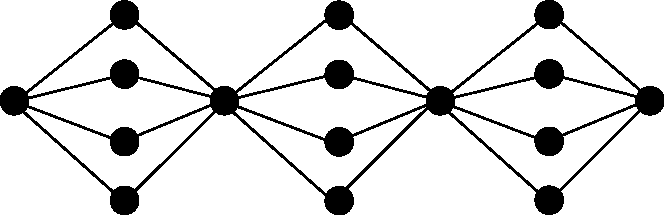
\includegraphics[scale=0.3]{fanout}
\end{center}
To avoid the spurious forking and joining, we {\it delay} the non-determinism
until and unless it is needed in {\it strict contexts} (such as the guard for an
{\tt if} a called procedure, or a numerical primitive application). 
%
Doing so collapses these forks and joins into a linear sequence of states:
\begin{center}

\includegraphics[scale=0.3]{lazy}
\end{center}

This shift does not change the concrete semantics of the language to
be lazy.  Rather, it abstracts over transitions that the original
non-deterministic semantics steps through.
%
We say the abstraction is \emph{lazy} because it delays splitting on
the values in an address until they are \emph{needed} in the
semantics. It does not change the execution order that leads to the
values that are stored in the address.

We introduce a new kind of value,
\spchoice
{$\saddr{\maddr}$}
{$\superposition{\mval{s}}$ (for ``superposition'')},
%
that represents a delayed non-deterministic choice of a value from
\spchoice
{$\msto(\maddr)$}
{$\mval{s}$}.
%
The following rules highlight the changes to the semantics:

\renewcommand{\ext}{\mathit{ext}}

\begin{align*}
\spchoice
{\force &: \Store \times \Value \to \Set(\Value) \\
 \force(\msto,\saddr{\maddr}) &= \msto(\maddr) \\
 \force(\mval) &= \{\mval\}}
{\force &: \Value \to \Set(\Value) \\
 \force(\superposition{\mval{s}}) &= \mval{s} \\
 \force(\mval) &= \{\mval\}}
\\
%
\ev{\svar{\mvar},\menv,\mkont,\msto} &\lmachstep\;
\spchoice
{\co{\mkont,\saddr{\menv(\mvar)},\msto}}
{\co{\mkont,\superposition{\msto(\menv(\mvar))},\msto}} \\
%
\co{\kar[^\mcntr_\mlab]{\mexp,\menv,\maddr_\mkont},\mval,\msto}
&\lmachstep\;
\ev[^\mcntr]{\mexp,\menv,\msto',\kfn[^\mcntr_\mlab]{\maddr_f,\maddr_\mkont}} \\
\text{ where }
\maddr_f &= \alloc(\mstate) \\
\msto' &=
\spchoice
{\msto \sqcup[\maddr \mapsto \force(\msto,\mval)]}
{\msto \sqcup[\maddr \mapsto \force(\mval)]} \\
%
\co{\kif[^\mcntr]{\mexpi0,\mexpi1,\menv,\maddr_\mkont},\mval,\msto}
&\lmachstep\;
\ev[^\mcntr]{\mexpi,\menv,\msto,\mkont} \\
\text{ if } \mkont &\in \msto(\maddr_\mkont),
            \strue \in \spchoice{\force(\msto,\mval)}{\force(\mval)}
\end{align*}
Since {\tt if} guards are in strict position, we must force the value
to determine which branch to to take. The middle rule uses $\force$
only to combine with values in the store - it does not introduce
needless non-determinism.

\spchoice{
\noindent
We have two choices for how to implement lazy non-determinism.

\paragraph{Option 1: Lose precision; simplify implementation}
This semantics introduces a subtle precision difference over the
baseline. Consider a configuration where a reference to a variable and
a binding of a variable will happen in one step, since store widening
leads to stepping several states in one big ``step.'' With laziness,
the reference will mean the original binding(s) of the variable or the
new binding, because the actual store lookup is delayed one step
(i.e. laziness is administrative). Without laziness, the reference
will fan out to all the bindings of the variable before the new
binding happens and thus theoretically has an observable precision
difference. % All our benchmarks maintain their precision with lazy non-determinism, however.

\paragraph{Option 2: Regain precision; complicate implementation}
The administrative nature of laziness means that we could remove the
loss in precision by duplicating the reduction relation to specialize
variable lookup. This works since in the semantics of ISWIM with
store-allocated results consumes the value component of states in one
step. This is not the case for semantics that replicate the value
component across reductions, say for popping off exception handler
frames. Further convolution is needed to remove the administrative
nature of laziness in these semantics. Due to the increase of
conceptual and implementation complexity for negligible benefit, we
decided against this approach.

\paragraph{Our choice: option 1}
The configurations that lead to precision loss happen too rarely to
warrant the significant increase in time and memory needed for this
eager non-determinism. Indeed, were the variable reference a step
later and another binding not made in that step, the results of the
two approaches are the same. Without a widened store, lazy
non-determinism is not a complete abstraction with either approach,
but the precision gains are not immediately apparent due to fake
rebinding (a second reference to the same variable chooses a different
value from the first) and other problems. The performance and memory
gains are apparent, so we favor the simplicity over invisible
gains.}{}

\spchoice
{
\begin{theorem}[Soundness]
  If $\mstate \machstep \mstate'$ and $\mstate \sqsubseteq
  \mastate$ then there exists a $\mastate'$ such that $\mastate
  \lmachstep \mastate'$ and $\mstate' \sqsubseteq \mastate'$
\end{theorem}
Here $\sqsubseteq$ is straightforward - the LHS store must be
contained in the RHS store, and if values occur in the states, forcing
the LHS value must be a subset of forcing the corresponding RHS value.
The proof is by cases on $\mstate \machstep \mstate'$.}
{
\begin{theorem}[Completeness]For all $\mexp$,
 $\traces_{\text{Lazy}}(\mexp)$ is a complete abstraction of $\traces_{\text{ISWIM}}(\mexp)$.
\end{theorem}
We have a statement about traces because we need induction to show no
cruft values are in superposition.  The induction hypothesis tells us
that there are non-lazy traces that lead to all the values in
superposition, so when we take a lazy step, we are taking several
non-lazy steps, and we stay in sync. The other direction we just
collapse the superposition in each possibility to construct the
non-lazy traces.}

% Lazy:  cpu time: 32481 real time: 32881 gc time: 547

\subsection{Abstract compilation}

The prior optimization saved time by doing the same amount of
reasoning as before but in fewer transitions. We can exploit the same
idea---same reasoning, fewer transitions---with abstract
compilation. Abstract compilation transforms complex expressions whose
\emph{abstract} evaluation is deterministic into ``abstract
bytecodes.''  The abstract interpreter then does in one transition
what previously took many. In short, abstract compilation eliminates
unnecessary allocation, deallocation and branching. The technique is
precision preserving without store widening. We discuss the precision
differences with store widening at the end of the section.

The following example illustrates
the essence of abstract compilation effect:
\[
\mexp := \sapp{\sapp{\sapp\mvar{\mexp_1}}{\mexp_2}}{\mexp_3}
\]
makes the following transitions:
\begin{align}
& \ev[^\mcntr]{\sapp{\sapp{\sapp\mvar{\mexp_1}}{\mexp_2}}{\mexp_3},\menv,\msto_0,\mkont}\\
\machstep\; &
\ev[^{\mcntr'}]{\sapp{\sapp\mvar{\mexp_1}}{\mexp_2},\menv,\msto_1,\kar{\mexp_3,\menv,\maddr_{f1},\maddr_{a1},\maddr_1}}
\\
\machstep\; &
\ev[^{\mcntr''}]{\sapp\mvar{\mexp_1},\menv,\msto_2,\kar{\mexp_2,\menv,\maddr_{f2},\maddr_{a2},\maddr_2}}
\\
\machstep\; &
\ev[^{\mcntr'''}]{\mvar, \menv,\msto_3,\kar{\mexp_1,\menv,\maddr_{f3},\maddr_{a3},\maddr_3}} % {\mexp_2}
\\
\machstep\; &
\spchoice
{\co{\kar{\mexp_1,\menv,\maddr_{f3},\maddr_{a3},\maddr_3},\saddr{\menv(\mvar)},\msto_4}}
{\co{\kar{\mexp_1,\menv,\maddr_{f3},\maddr_{a3},\maddr_3},\superposition{\msto_4(\menv(\mvar))},\msto_4}}
\end{align}
where \(
\msto_4 = \msto_0 \sqcup [\maddr_1 \mapsto \setof{\mkont},
\maddr_2 \mapsto \setof{\kar{\compile{\mexp_3},\menv,\maddr_1}},
\maddr_3 \mapsto \setof{\kar{\compile{\mexp_2},\menv,\maddr_2}}]\).

Whereas abstract compilation gives us in one step:
\begin{align*}
\compile{\mexp}^\mcntr(\menv,\msto_0,\mkont) = 
\spchoice
{\co{\kar{\compile{\mexp_1},\menv,\maddr_{f3},\maddr_{a3},\maddr_3},\saddr{\menv(\mvar)},\msto'_4}}
{\co{\kar{\compile{\mexp_1},\menv,\maddr_{f3},\maddr_{a3},\maddr_3},\superposition{\msto'_4(\menv(\mvar))},\msto'_4}}
\end{align*}
where \(
\msto'_4 = \msto_0 \sqcup \{ [\maddr_1 \mapsto \{ \mkont \}],
[\maddr_2 \mapsto \kar{\compile{\mexp_3},\menv,\maddr_1}],
[\maddr_3 \mapsto \kar{\compile{\mexp_2},\menv,\maddr_2}]\).

The compilation step converts expressions into functions that expect
the other components of the {\tt ev} state. Its definition in figure
\ref{fig:compile} shows close similarity to the rules for interpreting
{\tt ev} states. The next step is to change reduction rules that
create {\tt ev} states to instead call these functions. Figure
\ref{fig:caam} shows the modified reduction relation. The only change
from the previous semantics is that $\ev{}$ state construction is
replaced by calling the compiled expression. For notational coherence,
we write $\lambda^\mcntr(\mathit{args} \ldots)$ for
$\lambda(\mathit{args} \ldots, \mcntr)$ and
$\mcomp^\mcntr(\mathit{args}\ldots)$ for $\mcomp(\mathit{args}\ldots,
\mcntr)$.

\begin{figure}
\begin{align*}
\compile{\_} &: (\Expr \to \Env \times \Store \times \Kont \times \Counter) \to \State \\
\mcntr' &= \tick(\mlab,\menv,\msto,\mcntr) \\
\compile{\svar\mvar} &=
 \lambda^\mcntr(\menv,\msto,\mkont) .
\spchoice
{\co{\mkont,\saddr{\menv(\mvar)},\msto}}
{\co{\mkont,\superposition{\msto(\menv(\mvar))},\msto}}
\\
\compile{\slit\mlit} &= \lambda^\mcntr(\menv,\msto,\mkont) .
\co{\mkont,\mlit,\msto}
\\
\compile{\slam\mvar\mexp} &= \lambda^\mcntr(\menv,\msto,\mkont) .
\co{\mkont,\clos{\mvar,\compile{\mexp},\menv},\msto}
\\
\compile{\sapp[^\mlab]{\mexpi0}{\mexpi1}} &= \lambda^\mcntr(\menv,\msto,\mkont) .
\compile{\mexpi0}^{\mcntr'}(\menv,\msto',\kar[_\mlab^\mcntr]{\compile{\mexpi1},\menv,\maddr_\mkont})
\\
&\setlength\arraycolsep{5pt}
\begin{array}{lrl}
\text{ where } & \maddr_\mkont = \allockont^\mcntr_\mlab(\msto,\mkont) \\
               & \msto' = \msto\sqcup[\maddr_\mkont \mapsto \setof{\mkont}]
\end{array}
\\
\compile{\sif[^\mlab]{\mexpi0}{\mexpi1}{\mexpi2}} &= \lambda^\mcntr(\menv,\msto,\mkont) .
\compile{\mexpi0}^{\mcntr'}(\menv,\msto',\kif[^\mcntr]{\compile{\mexpi1},\compile{\mexpi2},\menv,\maddr})
\\
&\text{ where }\maddr_\mkont = \allockont^\mcntr_\mlab(\msto,\mkont) \\
&\phantom{\text{ where }} \msto' = \msto\sqcup[\maddr_\mkont \mapsto \setof{\mkont}]
\end{align*}
\caption{Abstract compilation}
\label{fig:compile}
\end{figure}

\begin{figure}
\begin{gather*}
\begin{align*}
\traces(\mexp) &= \{ \compile{\mexp}^\mtcntr(\epsilon,\varnothing,\varnothing,\kmt) \multimachstep \mstate \} \text{ where }
\end{align*}
\\[2mm]
\begin{align*}
%% CONTINUE
\co{\kmt,\mval,\msto} &\cmachstep
\ans{\msto,\mval'} \text{ if } \mval' \in \spchoice{\force(\msto,\mval)}{\force(\mval)}
\\
\co{\kar[^\mcntr_\mlab]{\mcomp,\menv,\maddr_\mkont},\mval,\msto} & \cmachstep
\mcomp^\mcntr(\menv,\msto',\kfn[^\mcntr_\mlab]{\maddr_f,\maddr_\mkont}) \\
\text{ where } \maddr_f &= \alloc(\mstate) \\
               \msto' &= \msto\sqcup[\maddr_f \mapsto \spchoice{\force(\msto,\mval)}
                                                               {\force(\mval)}]
\\
\co{\kfn[^\mcntr_\mlab]{\maddr_f,\maddr_\mkont},\mval,\msto} & \cmachstep
\ap[^\mcntr_\mlab]{\mval,\mval\mkont,\msto} \\
\text{ if }\mval &\in \msto(\maddr_f), \mkont \in \msto(\maddr_\mkont) \\
\\
\co{\kif[^\mcntr]{\mcompi0,\mcompi1,\menv,\maddr},\strue,\msto} & \cmachstep
\mcompi0^\mcntr(\menv,\msto,\mkont)
\text{ if }\mkont\in\msto(\maddr)
\\
\co{\kif[^\mcntr]{\mcompi0,\mcompi1,\menv,\maddr},\sfalse,\msto} & \cmachstep
\mcompi1^\mcntr(\menv,\msto,\mkont)
\text{ if }\mkont\in\msto(\maddr)
\\[2mm]
%% APPLY
\ap[^\mcntr_\mlab]{\clos{\mvar,\mcomp,\menv},\mval,\msto,\mkont} & \cmachstep
\mcomp^{\mcntr'}(\menv',\msto',\mkont) \\
\text{ where }\menv' &= \menv[\mvar\mapsto\maddr] \\
              \msto' &= \msto\sqcup[\maddr\mapsto \spchoice{\force(\msto,\mval)}{\force(\mval)}]
\\
\ap{\mop,\mval,\msto,\mkont} & \cmachstep
\co{\mkont,\mval',\msto} \\
\text{ where } \mvalx{u} &\in \spchoice{\force(\msto,\mval)}{\force(\mval)}, \mval'\in\interpdelta(\mop,\mvalx{u})
\end{align*}
\end{gather*}
\caption{Abstract abstract machine for compiled ISWIM}
\label{fig:caam}
\end{figure}

\paragraph{Correctness}
The correctness of abstract compilation seems obvious, but it has
never before been rigorously proved. What constitutes correctness in
the case of dropped states, anyway? Applying an abstract bytecode's
function does many ``steps'' in one go, at the end of which, the two
semantics line up again (modulo representation of expressions). This
constitutes the use of a notion of stuttering. We therefore prove a
stuttering bisimulation~\cite{ianjohnson:BCG88} between this
semantics and the previous section's to show precision preservation.

The number of transitions that can occur in succession from an
abstract bytecode is roughly bounded by the amount of expression
nesting in the program. The partial order that defines subexpressions
smaller than the expression in which they occur is well-founded, so we
use this observation to drive our use of a well-founded equivalence
bisimulation (WEB)~\cite{ianjohnson:manolios-diss}. WEBs are equivalent to the notion of a stuttering
bisimulation, but are more amenable to mechanisation (and thus
rigorous proof). They also only require reasoning over one step of the
reduction relation, which makes the proof concise.

We define a refinement from non-compiled to compiled states by
``committing'' all the actions of an $\ev{}$ state (defined similarly to
$\compile{\_}$, but immediately applies the functions), and
subsequently changing all expressions with their compiled
variants. Since WEBs are for single transition systems, a WEB
refinement is over the disjoint union of our two semantics, and the
equivalence relation we use is just that a state is related to its
refined state (and itself). Call this relation $B$.

Before we prove this setup is indeed a WEB, we need one lemma that
applying an abstract bytecode's function is equal to refining the
corresponding $\ev{}$ state:
%
\begin{lemma}[Compile/commit]\hfill\\
$\compile{\mexp}^\mcntr(\menv,r(\msto),r(\mkont)) = r(\ev[^\mcntr]{\mexp,\menv,\msto,\mkont})$.
\end{lemma}
The proof is by induction on $\mexp$.

\begin{theorem}[Precision preservation]
$B$ is a WEB on $\lmachstep \cup \cmachstep$
\end{theorem}

The full proof is in the appendix, but it follows by cases on
$\lmachstep \cup \cmachstep$ with the WEB \emph{witness} being the
well-order on expressions (with a $\bot$ element), and the following
$\erankt$, $\erankl$ functions:

\begin{align*}
\erankt(\ev[^\mcntr]{\mexp,\menv,\msto,\mkont}) &= \mexp \\
\erankt(\mstate) &= \bot \quad \text{otherwise} \\
\erankl(s,s') &= 0
\end{align*}
All cases are either simple steps or appeals to the well-order on $\erankt$'s range. The other rank function,
$\erankl$ is unnecessary, so we just make it the constant 0
function. The $\cmachstep$ cases are trivial.

\paragraph{Wide store and abstract compilation}
The fact that many changes happen in one step also makes the
comparison with the widened lazy semantics more subtle. It is possible
for different stores to occur between the different semantics because
abstract compilation can change the order in which the store is
changed. Consider the case where before we might call the same
function from two different places in 3 and 2 steps respectively,
compilation can make that 2 and 1, reversing the order that we bind
values in the store, leading to a mismatch from the previous
semantics. This kind of cross-step store poisoning is inevitable when a
store is shared between several traces. The binding could have just as
easily been observed the other way around in the non-compiled
semantics.

% Compile: cpu time: 255397 real time: 261532 gc time: 2947

% \noindent
% Compile + Lazy: cpu time: 31173 real time: 31642 gc time: 739

%\newpage

\subsection{Locally log-based store deltas}

Every step the analysis makes for the above techniques requires
joining entire (large) stores together. Not every step will modify all
addresses of the store, so joining entire stores is wasteful in terms
of memory and time. We can instead log store changes and replay the
change log on the full store after all steps have completed. This uses
far fewer join operations, leading to less overhead, and is precision-preserving.

We represent change logs as $\msdiff \in \StoreDelta = (\Addr \times
  \Set(\Storeable))^*$. Each $\msto\sqcup[\maddr \mapsto \mval{s}]$
 becomes a log addition
$\cons{\ttuple{\maddr}{\mval{s}}}{\msdiff}$, where $\msdiff$ begins
empty ($\mtlst$) for each step. Applying the changes to the full store
is straightforward:
\begin{align*}
\replay &: \StoreDelta \times \Store \to \Store \\
\replay(\left[ \ttuple{\maddr_i}{\mval{s_i}}, \ldots\right], \msto) &= \msto \sqcup [\maddr_i \mapsto \mval{s_i}] \sqcup \ldots
\end{align*}
%\replay(\mtlst, \msto) &= \msto \\
%\replay(\cons{\ttuple{\maddr}{\mval{s}}}{\msdiff}, \msto) &= \replay(\msdiff, \msto\sqcup[\maddr \mapsto \mval{s}])

The transition relation is identical except for the addition of this change log.
%
We maintain the invariant that lookups will never rely on the change log, so we can use the originally supplied store unmodified:

\begin{align*}
(\ap[^\mcntr_\mlab]{\clos{\mvar,\mexp,\menv},\mval,\mkont},\msto,\msdiff) & \dmachstep
(\ev[^{\mcntr'}]{\mexp,\menv',\mkont},\msdiff') \\
\text{ where }\menv' &= \menv[\mvar\mapsto\maddr] \\
              \msdiff' &= 
\spchoice
{\cons{\ttuple{\maddr}{\force(\msto,\mval)}}{\msdiff}}
{\cons{\ttuple{\maddr}{\force(\mval)}}{\msdiff}}
\end{align*}

Compilation changes to additionally take a $\msdiff$ component, so the
above rule's right hand side would instead be $k^{\mcntr'}(\menv',
\msto, \msdiff', \mkont)$ where $k = \compile{e}$ would be in the closure.

\spchoice{ }{
\paragraph{Caveat:} With abstract compilation, in one step, we can
both bind a variable and reference it. This breaks the invariant of
not relying on the change log. The problem is that the store does not
change until all steps are done, so the reference unsoundly returns
the previous binding (or nothing at all)! There are a couple ways to
address this. One way is to make all compiled forms that reference the
store into a new kind of state that has to be stepped in order to
reference the store and continue. Another way is to make function
application take one extra step after binding, so that running the
body of the function sees the changed store. The latter is the more
enticing of the two, since programs have more variable references than
function calls - we don't want to slow them down if we don't have
to. This change is also minutely different in precision, so we don't
have complete abstraction. If the lazy semantics delayed the lookup of
a variable's address to put in superposition (i.e., produced
$\saddr{\menv(\mvar)}$ instead of
$\superposition{\msto(\menv(\mvar))}$, and $\force$ additionally takes
a $\msto$), then the lazy semantics loses its complete abstraction,
but this current caveat disappears.
}

We lift $\dmachstep$ to accommodate for the asymmetry
in the input and output. For each state that is stepped, we feed the
output changes to the next so that all changes get accumulated:

\begin{align*}
(S, F, \msto) &\mathrel{\damachstep} (S \cup S', F', \msto') \\
\mbox{ where }
 (F', \msdiff') &= \step^*(\varnothing, F, \msto, \epsilon) \\
 \msto' &= \replay(\msdiff',\msto) \\
               S' &= \setof{(c,\msto') \mid c \in F'} \\
\step^*(F', \varnothing, \msdiff) &= (F', \msdiff) \\
\step^*(F', \{c\}\cup F, \msdiff) &= \step^*(F'\cup \states^*, F, \msdiff^*) \\
\states^* &= \{c' \mid (c,\msto,\msdiff) \dmachstep (c',\msdiff^c) \} \\
\msdiff^* &= \appendall(\setof{\msdiff^c \mid (c, \msto,\msdiff) \dmachstep (c', \msdiff^c)}) \\
\appendall(\varnothing) &= \epsilon \\
\appendall(\setof{\msdiff}\cup\Xi) &= \append(\msdiff,\appendall(\Xi))
\end{align*}

Here $\appendall$ combines change logs across all non-deterministic
steps for a state to later be replayed. The order the combination
happens in doesn't matter, because join is associative and
commutative.

% Here $\replayall : \Set(\StoreDelta) \times \Store \to \Store$ replays all logs in a set on top of the given store. Since join is associative and commutative, the order does not matter:
% \begin{align*}
%   \replayall(\varnothing,\msto) &= \msto \\
%   \replayall(\setof{\msdiff} \cup \Xi, \msto) &= \replayall(\Xi, \replay(\msdiff, \msto))
% \end{align*}

Correctness here requires a lemma that relates the differences in the compilation functions.
\begin{lemma}[Compile coherence]
Let $\dcompile{\mexp}^\mcntr(\menv,\msto,\msdiff,\mkont) = \ttuple{\mastate}{\msdiff'}$
and $\compile{\mexp}^\mcntr(\menv,\msto^*,\mkont^*) = \wn(\mastate',\msto^{*'})$.
If $\msto \equiv \msto^*$, $\msdiff \equiv \msdiff^*$, and $\mkont \equiv \mkont^*$, then
$\mastate' \equiv \mastate$
and there exists an $\msdiff''$ such that \\
   $\replay(\msdiff'',\replay(\msdiff^*,\msto^*)) \equiv \replay(\msdiff',\msto)$.
\end{lemma}
Here $\equiv$ means structurally the same, only compiled expressions
are compiled with the updated compilation function that builds store
deltas. Proof is by induction on $\mexp$.

\begin{theorem}[Equivalence with wide abstract compilation]
If $S \equiv S^*, F \equiv F^*, \msto \equiv \msto^*$, then
$(S,F,\msto) \machstep (S',F',\msto')$ iff
$\exists S^*_1, F^*_1, \msto^*_1.
  S' \equiv S^*_1 \wedge F' \equiv F^*_1 \wedge \msto' \equiv \msto^*_1 \wedge
  (S^*,F^*,\msto^*) \dmachstep (S^*_1,F^*_1,\msto^*_1)$
\end{theorem}
Proof by the above lemma and that replaying in any order is equivalent
(associativity and commutativity of $\sqcup$).

%% Delta Store +k Compile + Lazy:
%%    cpu time: 668 real time: 686 gc time: 41

\subsection{Imperative, preallocated data structures}

Thus far, we have made our optimizations in a purely functional
manner. For the final push for performance, we need to dip into the
imperative. In this section, we show an alternative representation of
the store and seen set that are more space-efficient and are amenable
to destructive updates.

The following transfer function has several components that can be
destructively updated, and intermediate sets can be elided by adding
to global sets. In fact, the log of store deltas can be removed as
well, by updating the store in-place, and on lookup, using the first
value timestamped $\le$ the current timestamp. We start with the
purely functional view.

\subsubsection{Pure setup for imperative implementation}

The store maps to a stack of timestamped sets of abstract values.

\begin{align*}
\msto \in \Store &= \Addr \to \Valstack \\
\mvalstack \in \Valstack &= (\Timestamp \times \wp(\Storeable))^*
\end{align*}

Here we formally define what lookup and update mean at a given
timestamp.

\begin{align*}
\lookup(\mvalstack,t) &=
  \left\{
    \begin{array}{ll}
      \mval{s} & \text{ if } \mvalstack = \cons{\ttuple{t'}{\mval{s}}}{\mvalstack'}, t' \le t \\
      \mval{s'} & \text{ if } \mvalstack = \cons{\ttuple{t'}{\mval{s}}}{\cons{\ttuple{t''}{\mval{s'}}}{\mvalstack'}}, t' > t
    \end{array}\right. \\
\msto \sqcup_t [\maddr \mapsto \mval{s}] &= \msto[\maddr \mapsto \mvalstack],\changep \\
 (\mvalstack,\changep) &= \msto(\maddr)\sqcup_t \mval{s} \\
\epsilon \sqcup_t \mval{s} &= \ttuple{t}{\mval{s}} \\
\cons{\ttuple{t'}{\mval{s}}}{\mvalstack} \sqcup_t \mval{s'} &= \cons{\ttuple{t'}{\mval{s}\sqcup\mval{s'}}}{\mvalstack},\strue \text{ if } t' > t \\
\mvalstack \sqcup_t \mval{s} &= \cons{\ttuple{t+1}{\mval{s^*}}}{\mvalstack},\strue
           \text{ if } \mval{s'} \neq \mval{s^*} \\
 \mval{s'} &= \lookup(\msto(\maddr),t) \\
 \mval{s^*} &= \mval{s} \sqcup \mval{s'} \\
\mvalstack \sqcup_t \mval{s} &= \mvalstack,\sfalse \text{ otherwise}
\end{align*}

For the purposes of space, we reuse the $\dmachstep$ semantics and change the definition $\replay$ to track if the store has changed, in order to increment the global timestamp.
\begin{align*}
\replay_t(\epsilon,\msto,\changep) &= \msto,\changep \\
\replay_t(\cons{\ttuple{\maddr}{\mval{s}}}{\msdiff},\msto,\changep) &= \replay_t(\msdiff,\msto',\changep \vee \changep') \\
\text{ where } (\msto',\changep') &= \msto\sqcup_t[\maddr \mapsto, \mval{s}] \\
\replayall_t(\varnothing,\msto,\changep) &= \msto,\changep \\
\replayall_t(\setof{\msdiff}\cup\Xi,\msto,\changep) &= \replayall_t(\Xi, \msto', \changep') \\
\text{ where } (\msto',\changep') &= \replay_t(\msdiff,\msto,\changep)
\end{align*}

Because the store has all the temporal information baked into it, we
rephrase the core semantics in terms of a transfer function. The least
fixed-point of this function gives a more compact representation of
the reduction relation of the previous section.

\begin{align*}
\System &= (\State \to {\Timestamp}^*) \times \wp(\State) \times \Store \times \Timestamp \\
{\mathcal F} &: \System \to \System \\
{\mathcal F}(S,F, \msto,t) &= (S',F',\msto', t') \\
\text{ where }
I &= \setof{(\mstate',\msdiff') \mid
       \mstate \in F,
       (\mstate,\msto^*,\epsilon) \dmachstep
       (\mstate',\msdiff')} \\
\msto^* &= \lambda \maddr.\lookup(\msto(\maddr),t) \\
(\msto',\changep) &= \replayall_t(\setof{\msdiff \mid (\_,\msdiff) \in I},\msto,\sfalse) \\
t' &= \left\{\begin{array}{ll} t+1 & \text{ if } \changep \\
              t   & \text{ otherwise}
             \end{array}\right. \\
F' &= \setof{\mstate \mid (\mstate,\_) \in I, \changep \vee S(\mstate) \neq \cons{t}{\_}} \\
S' &= \lambda \mstate. \left\{\begin{array}{ll}
                               \cons{t'}{S(\mstate)} & \text{ if } \mstate \in F' \\
                               S(\mstate) & \text{ otherwise}
                             \end{array}\right.
\end{align*}

We increase the timestamp only if we find that the store has changed
from any join operation. The frontier set only gets states that we
haven't seen at the next timestamp. The states we've seen gets updated
with the frontier states at the next timestamp. We prove semantic
equivalence with the previous semantics with a lock-step bisimulation with the stack of stores abstraction,
which follow from equational reasoning from the following lemmas:

\begin{lemma}[Store of value stacks completely abstracts stack of stores]
TODO
\end{lemma}

\begin{lemma}[$\changep$ means change]
  If $\replayall_t(\Xi,\msto,\changep) = \msto',\changep'$ then
  $\msto' = \replay(\appendall(\Xi),\msto)$ and $\changep \vee
  (\changep' \iff \msto \neq msto')$.
\end{lemma}
By induction on the size of $\Xi$.

\begin{theorem}[Timestamped system with stack of stores completely abstracts wide store deltas]
TODO
\end{theorem}

\subsubsection{Pure to imperative}

The intermediate data structures of the above transfer function can all be streamlined into globals that are destructively updated. In particular, there are 5 globals:

\begin{enumerate}
\item{$S$: the \emph{seen} set, though made a map for faster membership tests and updates.}
\item{$F$: the \emph{frontier} set, which must be persisent or copied for the iteration through the set to be correct.}
\item{$\msto$: the store, which represents all stores that occur in the reduction semantics.}
\item{$t$: the timestamp, or length of the store chain - all stores that occur in the semantics are totally ordered due to single-threading the store.}
\item{$\changep$: whether there has been a store change stepping all states in $F$.}
\end{enumerate}

The reduction relation would then instead of building store deltas,
update the global store. We would also not view it as a general
relation, but a function that adds all next states to $F$ if they have
not already been seen. At the end of iterating through $F$, $S$ is
updated with the new states at the next timestamp.

\subsubsection{Pre-allocating the store}

Internally, the algorithm at this stage uses hash tables to model the store.
%
This is because stores used to be distributed to all states, which
required a compact, dynamic representation.
%
But, such a dynamic structure isn't necessary when we know the
structure of the store in advance: we know all possible entries, and
we know its maximum size.

In a monovariant analysis, the domain of the store is
exactly the set of expressions in the program.
%
If we label each expression with a unique natural, the analysis can
index directly into the store without a hash or a collision.
%
Even for polyvariant analyses, it is possible to compute the maximum
number of addresses and similarly pre-allocate either the spine of the
store or (if memory is no concern) the entire store.

\section{Evaluation}
\label{sec:eval}

We have implemented, optimized, and evaluated an analysis framework
supporting higher-order functions, state, first-class control,
compound data, and a large number of primitive kinds of data and
operations such as floating point, complex, and exact rational
arithmetic.  The analysis is evaluated against a suite of Scheme benchmarks
drawn from the literature.
%
For each benchmark, we collect analysis times, peak memory usage, and
the rate of states-per-second explored by the analysis for each of the
optimizations discussed in section~\ref{sec:opt}, cumulatively
applied.  The analysis is stopped after consuming 30 minutes of time
or 1 gigabyte of space.  When presenting \emph{relative} numbers, we
use the timeout limits as a lower bound on the actual time required,
thus giving a conservative estimate of improvements.

All benchmarks are calculated as an average of 5 runs, done in
parallel, on an 12-core, 64-bit Intel Xeon machine running at 2.40GHz
with 12Gb of memory.

Many benchmarks cause the baseline analyzer to take longer than 30
minutes or to consume more 1 gigabyte of memory, at which point the
analysis is stopped.  This is the case for the largest benchmark
program, {\bf nucleic}, which is 3,500 lines of code and takes under a minute in the
most optimized analyzer.  For those benchmarks that did complete on
the baseline, the optimized analyzer outperformed the baseline by a
factor of two to three orders of magnitude.
% safer to not give exact factors
% 475 to 4,382.

We use the following set of benchmarks:
\begin{figure}
\centering
\begin{tabular}{@{}l|r|r|r|r|r|r|r@{}}
Program & LOC
& \multicolumn{2}{c|}{Time {\small (s)}}
& \multicolumn{2}{c|}{Space {\small (MB)}}
& \multicolumn{2}{c@{}}{Speed {\small (state/s)}}
\\
\hline\hline
nucleic & 3492 & \text{{\small $m$}} & 57.8 & \text{{\small $m$}} & 138 & \text{{\small $m$}} & 7K \\
matrix & 747 & \text{{\small $t$}} & 4.9 & \text{{\small $t$}} & 63 & \text{{\small $t$}} & 68K \\
nbody & 1435 & \text{{\small $t$}} & 38.3 & \text{{\small $t$}} & 124 & \text{{\small $t$}} & 53K \\
earley & 667 & 1.1K & 0.7 & 409 & 60 & 252 & 41K \\
maze & 681 & \text{{\small $t$}} & 4.0 & \text{{\small $t$}} & 60 & \text{{\small $t$}} & 80K \\
church & 42 & 44.9 & 0.2 & 86 & 60 & 714 & 43K \\
lattice & 214 & 348.5 & 0.4 & 231 & 60 & 382 & 72K \\
boyer & 642 & \text{{\small $m$}} & 18.3 & \text{{\small $m$}} & 93 & \text{{\small $m$}} & 33K \\
mbrotZ & 69 & 373.6 & 0.1 & 295 & 60 & 540 & 34K
\end{tabular}

\caption{Overview performance comparison between baseline and
  optimized analyzer (entries of \text{{\small $t$}} mean timeout, and \text{{\small $m$}} mean out of memory).}
\label{fig:bench-overview}
\end{figure}

\begin{enumerate}  %% Maybe use ``dictionary'' style enumeration.

\item {\bf nucleic}: a floating-point intensive application taken from
  molecular biology that has been used widely in benchmarking
  functional language
  implementations~\cite{dvanhorn:Hartel1996Benchmarking} and analyses
  (e.g.~\cite{dvanhorn:wright-jagannathan-toplas98,dvanhorn:jagannathan-etal-popl98}).
  It is a constraint satisfaction algorithm used to determine the
  three-dimensional structure of nucleic acids.

\item {\bf matrix} tests whether a matrix is maximal among all
  matrices of the same dimension obtainable by simple reordering of
  rows and columns and negation of any subset of rows and columns.  It
  is written in continuation-passing style (used in
  \cite{dvanhorn:wright-jagannathan-toplas98,dvanhorn:jagannathan-etal-popl98}).


\item {\bf nbody}: implementation~\cite{ianjohnson:nbody87} of the
  Greengard multipole algorithm for computing gravitational forces on
  point masses distributed uniformly in a cube (used in
  \cite{dvanhorn:wright-jagannathan-toplas98,dvanhorn:jagannathan-etal-popl98}).

\item {\bf earley}: Earley's parsing algorithm, applied to a 15-symbol
  input according to a simple ambiguous grammar.  A real program,
  applied to small data whose exponential behavior leads to a peak
  heap size of half a gigabyte or more during concrete execution.

\item {\bf maze}: generates a random maze using Scheme's {\tt
  call/cc} operation and finds a path solving
  the maze (used in
  \cite{dvanhorn:wright-jagannathan-toplas98,dvanhorn:jagannathan-etal-popl98}).

\item {\bf church}: tests distributivity of multiplication over
  addition for Church numerals (introduced by
  \cite{dvanhorn:Vardoulakis2011CFA2}).

\item {\bf lattice}: enumerates the order-preserving maps between two
  finite lattices (used in
  \cite{dvanhorn:wright-jagannathan-toplas98,dvanhorn:jagannathan-etal-popl98}).

\item {\bf boyer}: a term-rewriting theorem prover (used in
  \cite{dvanhorn:wright-jagannathan-toplas98,dvanhorn:jagannathan-etal-popl98}).

\item {\bf mbrotZ}: generates Mandelbrot set fractal using complex
  numbers.

\item {\bf graphs}: counts the number of directed graphs with a
  distinguished root and \(k\) vertices, each having out-degree at
  most 2. It is written in a continuation-passing style and makes
  extensive use of higher-order procedures---it creates closures
  almost as often as it performs non-tail procedure calls (used by
  \cite{dvanhorn:wright-jagannathan-toplas98,dvanhorn:jagannathan-etal-popl98}).
\end{enumerate}

%% 400 lines for the core, 700 lines for
%% abstraction over optimizations, 1500 lines for primitives and standard
%% list operations, 700 lines for instantiations to different
%% optimizations and 300 for parsing and macro transformers.

Figure~\ref{fig:bench-overview} gives an overview of the benchmark
results in terms of absolute time, space, and speed between the
baseline and most optimized analyzer.  Figure~\ref{fig:bench-all}
plots the factors of improvement over the baseline for each
optimization step. The dip we see in transition rate even though time
taken decreases is to be expected - fewer ``easy'' states are added by
abstract compilation. It increases again with the introduced
algorithmic improvements. Accumulating store changes in addition to
maintaining the store accounts for the higher memory usage when using
the store delta technique without further improvements.

\begin{figure*}
\begin{center}
  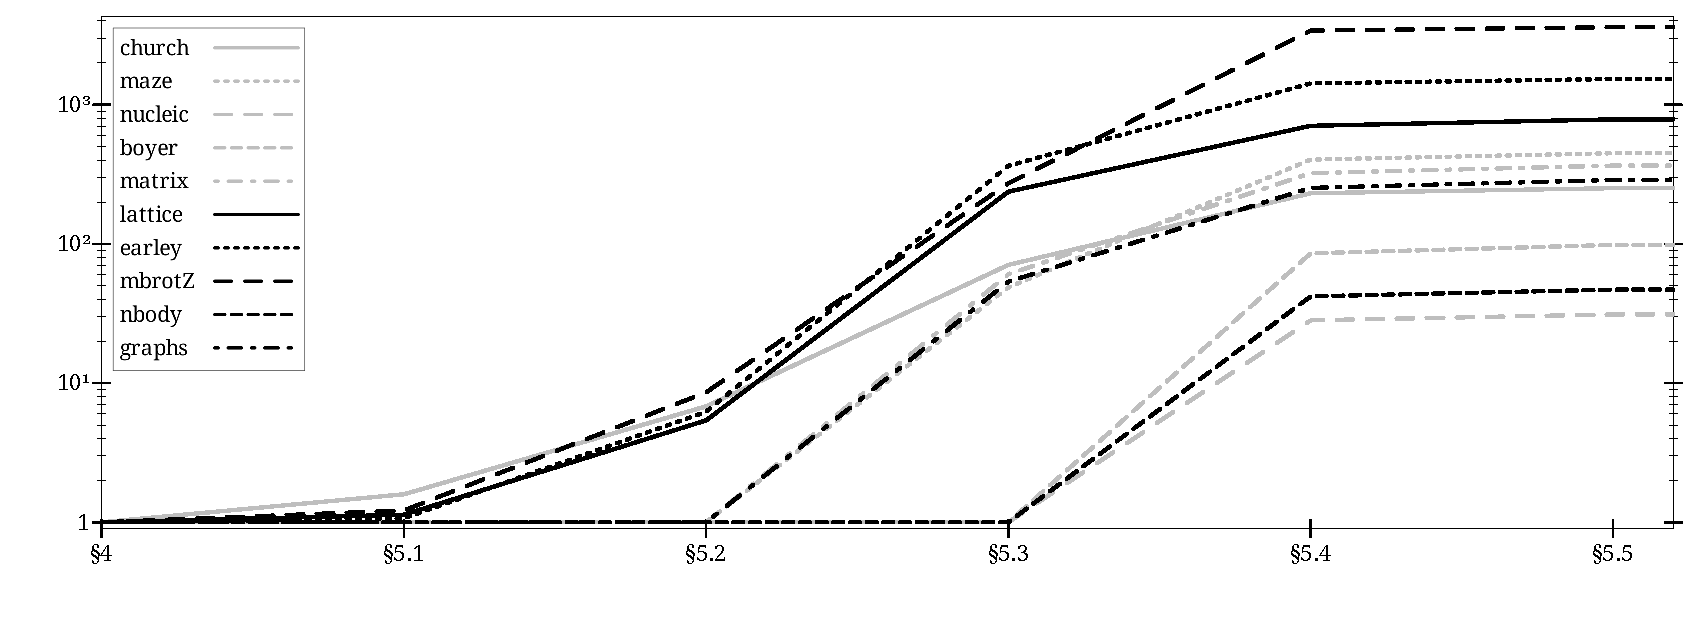
\includegraphics[width=6.5in]{all-relative-time}

  (a) Total analysis time

  \vspace{1em}
  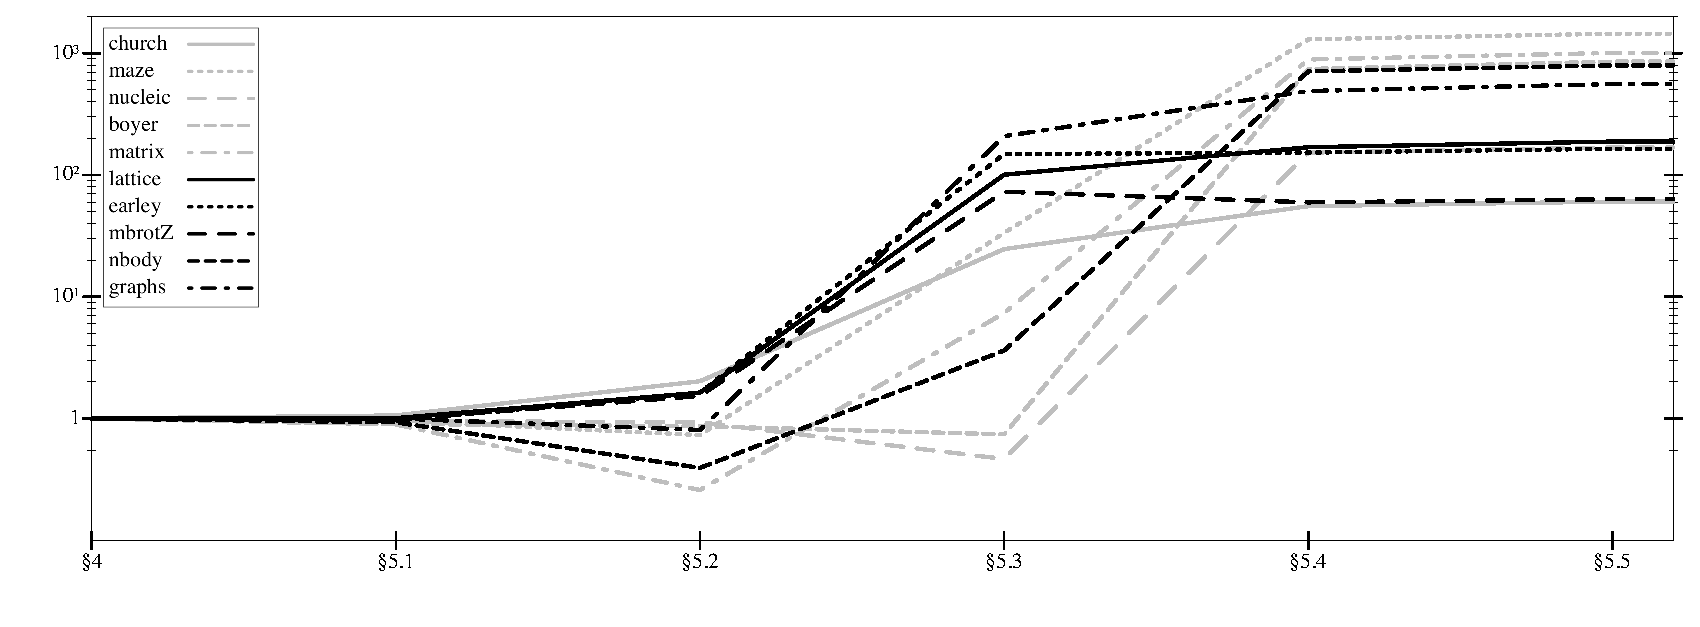
\includegraphics[width=6.5in]{all-relative-speed}

  (b) Rate of state transitions

  \vspace{1em}
  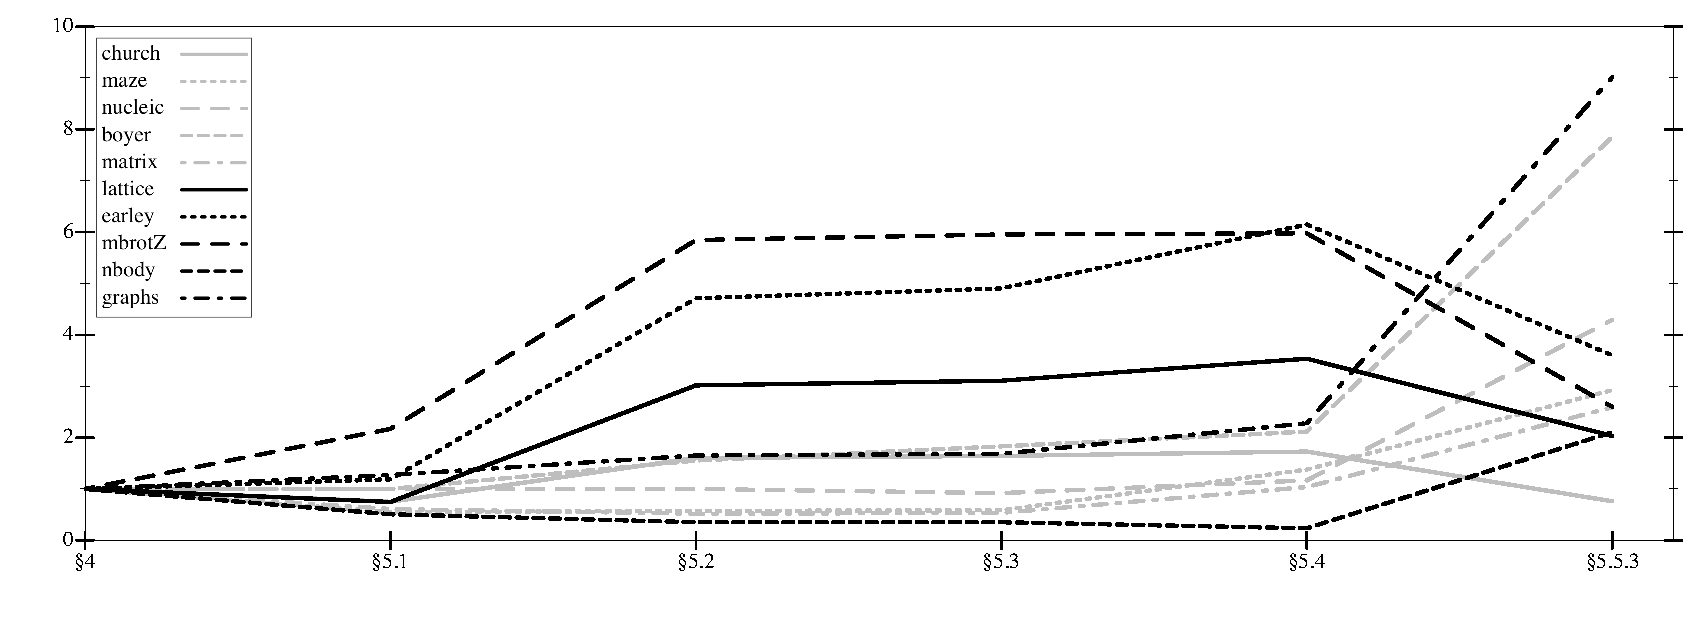
\includegraphics[width=6.5in]{all-relative-space}

  (c) Peak memory usage
\end{center}
\caption{Factors of improvement over baseline for each step of
  optimization (bigger is better).}
\label{fig:bench-all}
\end{figure*}

We evaluated the precision of these techniques with a singleton
variable analysis to find opportunities to inline constants and closed
functions. We found no change in the results across all
implementations, including Shivers' timestamp approximation.

Source code of the implementation and benchmark suite is at:

\begin{center}
\url{https://github.com/dvanhorn/oaam}
\end{center}

\paragraph{Comparison with other flow analysis implementations}

The analysis considered here computes results similar to Earl, et al.'s
0-CFA implementation~\cite{dvanhorn:Earl2012Introspective}, which
times out on the \Church{} benchmark because it does not widen the
store as described for our baseline evaluator.  So even though it
offers a fair point of comparison, a more thorough evaluation is
probably uninformative as the other benchmarks are likely to timeout
as well (and it would require significant effort to extend their
implementation with the features needed to analyze our benchmark
suite).  That implementation is evaluated against much smaller
benchmarks: the largest program is 30 lines.

Vardoulakis and Shivers evaluate their CFA2
analyzer~\cite{dvanhorn:Vardoulakis2011CFA2} against a variant of
0-CFA defined in their framework and the example we draw on is the
largest benchmark Vardoulakis and Shivers consider.  More work would
be required to scale the analyzer to the set of features required by
our benchmarks.

The only analyzers we were able to find that proved capable of
analyzing the full suite of benchmarks considered here were the Soft
Typing system of Wright and
Cartwright~\cite{dvanhorn:Wright1997Practical} and, in many ways its
successor, the Polymorphic splitting system of Wright and
Jagannathan~\cite{dvanhorn:wright-jagannathan-toplas98}.\footnote{This
  is not a coincidence; these papers set a high standard for
  evaluation, which we consciously aimed to approach.}  Unfortunately,
these analyses compute an inherently different and incomparable form
of analysis.  Consequently, we have omitted a complete comparison with
these implementations.  The AAM approach provides more precision in
terms of temporal-ordering of program states, which comes at a cost
that can be avoided in constraint-based approaches.  Consequently
implementation techniques cannot be ``ported'' between these two
approaches.  However, our optimized implementation is within an order
of magnitude of the performance of Wright and Jaganathan's analyzer.
Although we would like to improve this to be more competitive, the
optimized AAM approach still has many strengths to recommend it in
terms of precision, ease of implementation and verification, and rapid
design. We can get closer to their performance by relying on the
representation of addresses and the behavior of $\alloc$ to
pre-allocate most data structures and split the abstract store out
into parts that are more quickly accessed and updated. The first two
of our optimizations can still be applied to an analysis that does
abstract garbage collection~\cite{dvanhorn:Might:2006:GammaCFA},
whereas the polymorphic splitting implementation is tied strongly to a
single-threaded store.

\section{Related work}
\label{sec:related}

\paragraph{Abstracting Abstract Machines}

This work clearly closely follows Van Horn and Might's original papers
on abstracting abstract
machines~\cite{dvanhorn:VanHorn2011Abstracting,dvanhorn:VanHorn2012Systematic},
which in turn is one piece of the large body of research on flow
analysis for higher-order languages (see
Midtgaard~\cite{dvanhorn:Midtgaard2011Controlflow} for a thorough
survey).  The AAM approach sits at the confluence of two major lines
of research: (1) the study of abstract
machines~\cite{dvanhorn:landin-64} and their systematic
construction~\cite{dvanhorn:reynolds-hosc98}, and (2) the theory of
abstract interpretation
\cite{dvanhorn:Cousot:1977:AI,dvanhorn:Cousot1979Systematic}.


\paragraph{Frameworks for flow analysis of higher-order programs}

Besides the original AAM work, the analysis most similar to that
presented in section~\ref{sec:aam} is the infinitary control-flow
analysis of Nielson and Nielson~\cite{dvanhorn:nielson-nielson-popl97}
and the unified treatment of flow analysis by Jagannathan and
Weeks~\cite{dvanhorn:jagannathan-weeks-popl95}.  Both are
parameterized in such a way that in the limit, the analysis is
equivalent to an interpreter for the language, just as is the case
here.  What is different is that both give a constraint-based
formulation of the abstract semantics rather than a finite machine
model.

\paragraph{Abstract compilation}

Boucher and Feeley \cite{dvanhorn:Boucher1996Abstract} introduced the
idea of abstract compilation, which used closure generation
\cite{dvanhorn:Feeley1987Using} to improve the performance of control
flow analysis.  We have adapted the closure generation technique from
compositional evaluators to abstract machines and applied it to similar
effect.

\paragraph{Constraint-based program analysis for higher-order languages}

Constraint-based program analyses
(e.g.~\cite{dvanhorn:nielson-nielson-popl97,dvanhorn:wright-jagannathan-toplas98,dvanhorn:Meunier2006Modular,dvanhorn:steckler-wand-toplas97})
typically compute sets of abstract values for each program point.
These values approximate values arising at run-time for each
program point.  Value sets are computed as the least solution to a set
of (inclusion or equality) constraints.  The
constraints must be designed and proved as a sound approximation of
the semantics.  Efficient implementations of these kinds of analyses
often take the form of worklist-based graph algorithms for constraint
solving, and are thus quite different from the interpreter
implementation.  The approach thus requires effort in constraint
system design and implementation, and the resulting system require
verification effort to prove the constraint system is sound and that
the implementation is correct.

This effort increases substantially as the complexity of the analyzed
language increases.  Both the work of maintaining the concrete
semantics and constraint system (and the relations between them) must
be scaled simultaneously.  However, constraint systems, which have
been extensively studied in their own right, enjoy efficient
implementation techniques and can be expressed in declarative logic
languages that are heavily
optimized~\cite{dvanhorn:bravenboer-smaragdakis-oopsla09}.
Consequently, constraint-based analyses can be computed quickly.  For
example, Jagannathan and Wright's polymorphic splitting
implementation~\cite{dvanhorn:wright-jagannathan-toplas98} analyses
the \Church{} benchmark about 25 times faster than the fastest
implementation considered here.  These analyses compute very different
things, so the performance comparison is not apples-to-apples.

The AAM approach, and the state transition graphs it generates, encodes
temporal properties not found in classical constraint-based analyses
for higher-order programs.
%
Such analyses (ultimately) compute judgments on program terms and
contexts, e.g., at expression $e$, variable $x$ may have value $v$.
%
The judgments do not relate the order in which expressions and context
may be evaluated in a program, e.g., it has nothing
to say with regard to question like, ``Do we always evaluate $e_1$
before $e_2$?'' or ``Is it always the case that a file handle is
opened, read and then closed in that order?''
%
The state transition graphs can answer these kinds of queries, but
this does not come for free: respecting temporal order imposes an
order in which states and terms may be evaluated \emph{during} the
analysis.

\section{Conclusion}
\label{sec:conclusion}

Abstract machines are not only a good model for rapid analysis
development, they can be systematically developed into efficient
algorithms that can be proved correct. We view the primary
contribution of this work as a systematic path that eases the design,
verification, and implementation of analyses using the abstracting
abstract machine approach to within a factor of performant
constraint-based analyses.

%% \acks Sam Tobin-Hochstadt for encouragement and feedback -- he was
%% the first to prompt us to look into how make effective
%% implementations of the AAM approach.

%% Vincent St Amour and Mitchell Wand for feedback on early drafts.
%% Greg Morrisset and Matthias Felleisen for discussions.

%% NSF, DARPA


\paragraph{Acknowledgments}

We thank Suresh Jagannathan for providing source code to the
polymorphic splitting
analyzer~\cite{dvanhorn:wright-jagannathan-toplas98} and Ilya Sergey
for the introspective pushdown
analyzer~\cite{dvanhorn:Earl2012Introspective}.


\balance
\bibliographystyle{plain}
%\documentclass[preprint,onecolumn,9pt]{sigplanconf} %{onecol}
\usepackage{alltt,mathpartir}
\usepackage{amsmath,amsthm}
\usepackage{amssymb}
\usepackage{stmaryrd}
\usepackage{url}
\usepackage{graphicx}
\usepackage{balance}
\usepackage{calc}

\newtheorem{theorem}{Theorem}
\newtheorem{lemma}{Lemma}

\newcommand{\naive}{naive}
\newcommand{\naively}{naively}
\newcommand{\Naive}{Naive}
\newcommand{\Naively}{Naively}
% \usepackage{xltxtra}
% \setmonofont[Scale=MatchLowercase]{DejaVu Sans Mono}
%
\newcommand{\superscript}[1]{\ensuremath{^{#1}}}
\newcommand{\subscript}[1]{\ensuremath{_{#1}}}
\newcommand{\tuple}[3][\ ]{{\tt #2{#1}}({#3})}

% Values
\newcommand{\clos}[1]{\tuple{clos}{#1}}
\newcommand{\rlos}[1]{\tuple{rlos}{#1}}

% States
\newcommand{\ev}[2][\ ]{\tuple[#1]{ev}{#2}}
\newcommand{\co}[1]{\tuple{co}{#1}}
\newcommand{\ap}[2][\ ]{\tuple[#1]{ap}{#2}}
\newcommand{\ans}[1]{\tuple{ans}{#1}}

% Continuations
\newcommand{\kmt}{\tt mt}
\newcommand{\kar}[2][\ ]{\tuple[#1]{ar}{#2}}
\newcommand{\kfn}[2][\ ]{\tuple[#1]{fn}{#2}}
\newcommand{\kif}[2][\ ]{\tuple[#1]{fi}{#2}}
\newcommand{\kuop}[2][\ ]{\tuple[#1]{oa}{#2}}
\newcommand{\kbopa}[2][\ ]{\tuple[#1]{oa1}{#2}}
\newcommand{\kbopb}[2][\ ]{\tuple[#1]{oa2}{#2}}

% Implementation forms
\newcommand{\generator}{{\tt generator}}
\newcommand{\yield}[1]{{\tt yield} #1}

% Syntax
\newcommand{\syntax}[1]{{\tt #1}}
\newcommand{\sapp}[3][\ ]{\tuple[#1]{app}{#2,#3}}
\newcommand{\slam}[3][\ ]{\tuple[#1]{lam}{#2,#3}}
\newcommand{\srec}[4][\ ]{\tuple[#1]{rec}{#2,#3,#4}}
\newcommand{\svar}[2][\ ]{\tuple[#1]{var}{#2}}
\newcommand{\snum}[2][\ ]{\tuple[#1]{num}{#2}}
\newcommand{\sbln}[2][\ ]{\tuple[#1]{bool}{#2}}
\newcommand{\sif}[4][\ ]{\tuple[#1]{if}{#2,#3,#4}}
\newcommand{\sop}[2][\ ]{\tuple[#1]{op}{#2}}
\newcommand{\sopu}[3][\ ]{\tuple[#1]{op}{#2,#3}}
\newcommand{\sopb}[4][\ ]{\tuple[#1]{op2}{#2,#3,#4}}
\newcommand{\strue}{{\tt tt}}
\newcommand{\sfalse}{{\tt ff}}
\newcommand{\saddone}{{\tt add1}}
\newcommand{\ssubone}{{\tt sub1}}
\newcommand{\szerohuh}{\syntax{zero?}}
\newcommand{\szero}{\syntax{0}}
\newcommand{\slit}[2][\ ]{\tuple[#1]{lit}{#2}}

\newcommand{\sNum}{\syntax{Z}}

% Metavariables
\newcommand{\maddr}{a}
\newcommand{\mvar}{x}
\newcommand{\mvarf}{f}
\newcommand{\mexp}{e}
\newcommand{\mexpi}[1]{e_{#1}}
\newcommand{\mexpf}{f}
\newcommand{\menv}{\rho}
\newcommand{\mkont}{\kappa}
\newcommand{\msto}{\sigma}
\newcommand{\mop}{o}
\newcommand{\mval}{v}
\newcommand{\mnum}{z}
\newcommand{\mbln}{b}
\newcommand{\mvalx}[1]{#1}
\newcommand\machstep{\longmapsto}
\newcommand\multimachstep{\longmapsto\!\!\!\!\!\rightarrow}
\newcommand{\mlit}{l}
\newcommand{\mstate}{\varsigma}
\newcommand{\mcomp}{k}
\newcommand{\mcompi}[1]{\mcomp_{#1}}
\newcommand{\interpdelta}{\Delta}

\newcommand{\compile}[1]{\llbracket#1\rrbracket}

\newcommand{\mlab}{{\ell}}
\newcommand{\mcntr}{{\delta}}
\newcommand{\mtcntr}{{\epsilon}}


\begin{document}

\conferenceinfo{WXYZ '05}{date, City.}
\copyrightyear{2005}
\copyrightdata{[to be supplied]}

% \titlebanner{banner above paper title}        % These are ignored unless
% \preprintfooter{short description of paper}   % 'preprint' option specified.

%\title{Provably Correct, Low-Cost Optimizations for Abstract Abstract Machines}
\title{Correctly Optimizing Abstract Abstract Machines}

\authorinfo{J. Ian Johnson \and Nicholas Labich \and Matthew Might \and David Van Horn}
           {}
           {}
%% \authorinfo{J. Ian Johnson}
%%            {Northeastern University}
%%            {ianj@ccs.neu.edu}
%% \authorinfo{Nicholas Labich}
%%            {Northeastern University}
%%            {labichn@ccs.neu.edu}
%% \authorinfo{Matthew Might}
%%            {University of Utah}
%%            {might@cs.utah.edu}
%% \authorinfo{David Van Horn}
%%            {Northeastern University}
%%            {dvanhorn@ccs.neu.edu}
\maketitle

\begin{abstract}
The technique of \emph{abstracting abstract machines} (AAM) provides a
systematic approach for deriving computable approximations of
evaluators that are easily proved sound.
%
This article contributes a complementary step-by-step process for
subsequently going from a \naive{} analyzer derived under the AAM
approach, to an efficient and correct implementation.  The end result
of the process is a two to three order-of-magnitude improvement over
the systematically derived analyzer, making it competitive with
hand-optimized implementations that compute fundamentally less precise
results.
\end{abstract}

%% \category{CR-number}{subcategory}{third-level}

%% \terms
%% term1, term2

%% \keywords
%% keyword1, keyword2

\section{Introduction}

Program analysis provides sound predictive models of program behavior, but
in order for such models to be effective, they must be efficiently
computable and correct.  Past approaches to designing program analysis
have often featured abstractions that are far removed from the
original language semantics, requiring ingenuity in their construction
and effort in their verification.
%
The \emph{abstracting abstract machines} (AAM)
approach~\cite{dvanhorn:VanHorn2011Abstracting,dvanhorn:VanHorn2012Systematic}
to deriving program analyses provides an alternative: a systematic way
of transforming a programming language semantics in the form of an
abstract machine into a family of abstract interpreters.  It thus reduces
the burden of constructing and verifying the soundness of an abstract
interpreter.
%

%
% Specifically, these policies tune precision for control,
% the environment, the store, and base value domains.

By taking a
machine-oriented view of computation, AAM makes it possible to design,
verify, and implement program analyzers for realistic language
features typically considered difficult to model.  The approach was
originally applied to features such as higher-order functions,
stack inspection, exceptions, laziness, first-class continuations, and
garbage collection.  It has since been used to verify actor-
\cite{local:DOsualdo:12A} and
thread-based~\cite{dvanhorn:Might2011Family} parallelism and
behavioral contracts~\cite{dvanhorn:TobinHochstadt2012Higherorder}; it
has been used to model Coq~\cite{local:harvard},
Dalvik~\cite{local:dalvik}, Erlang~\cite{local:DOsualdo:12B},
JavaScript~\cite{local:DBLP:journals/corr/abs-1109-4467}, and
Racket~\cite{dvanhorn:TobinHochstadt2012Higherorder}.

The primary strength of the approach is that abstract interpreters can
be easily derived through a small number of steps from existing
machine models.  Since the relationships between abstract machines and
higher-level semantic models---such as definitional
interpreters~\cite{dvanhorn:reynolds-hosc98}, structured operational
semantics~\cite{dvanhorn:Plotkin1981Structural}, and reduction
semantics~\cite{dvanhorn:Felleisen2009Semantics}---are well
understood~\cite{dvanhorn:Danvy:DSc}, it is possible to navigate from
these high-level semantic models to sound program analyzers in a
systematic way.  Moreover, since these analyses so closely resemble a
language's interpreter (a) implementing an analysis requires little
more than implementing an interpreter, (b) a single implementation can
serve as both an interpreter and analyzer, and (c) verifying the
correctness of the implementation is straightforward.

Unfortunately, the AAM approach yields analyzers with poor performance
relative to hand-optimized analyzers.
%
Our work takes aim squarely at this ``efficiency gap,'' and narrows it
in an equally systematic way through a number of simple steps, many of
which are inspired by run-time implementation techniques such as
laziness and compilation to avoid interpretative overhead.  Each of
these steps is proven correct, so the end result is an implementation
that is trustworthy and efficient.

In this article, we develop a systematic approach to deriving a
practical implementation of an abstract-machine-based analyzer using
mostly semantic means rather than tricky engineering. Our goal is to
empower programming language implementers and researchers to explore
and convincingly exhibit their ideas with a low barrier to entry. The
optimizations we describe are widely applicable and apparently
effective to scale far beyond the size of programs typically considered
in the recent literature on flow analysis for functional languages.

\section{At a glance}

\begin{figure}[t]
\begin{center}
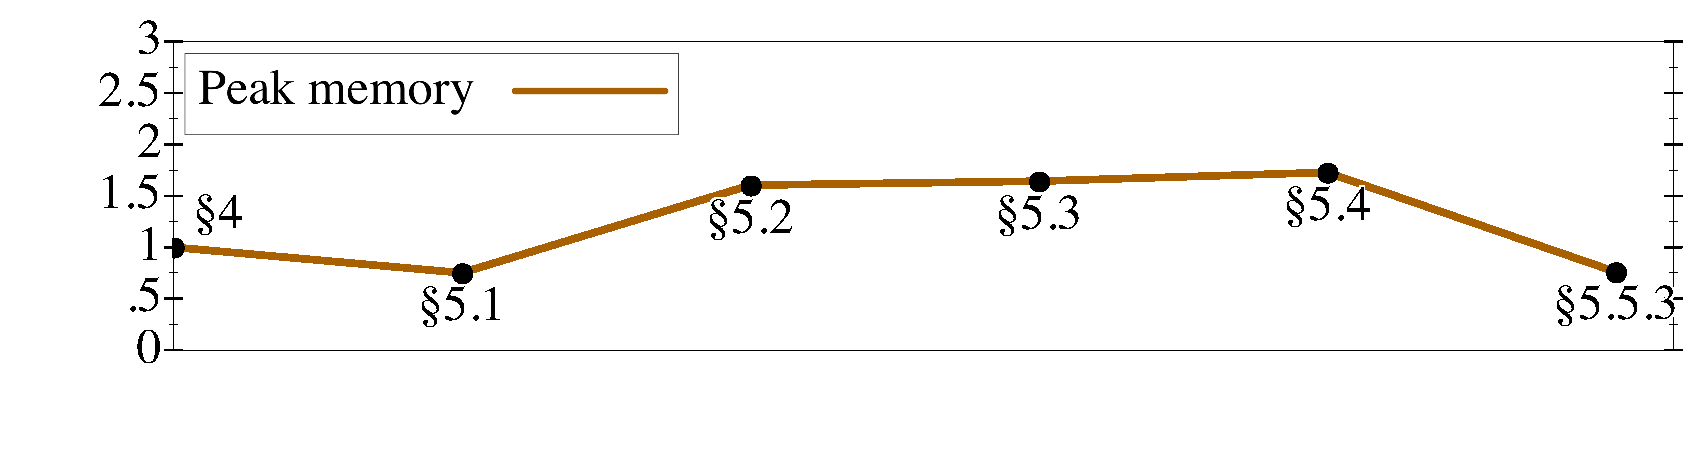
\includegraphics[width=3.2in]{church-relative-space}
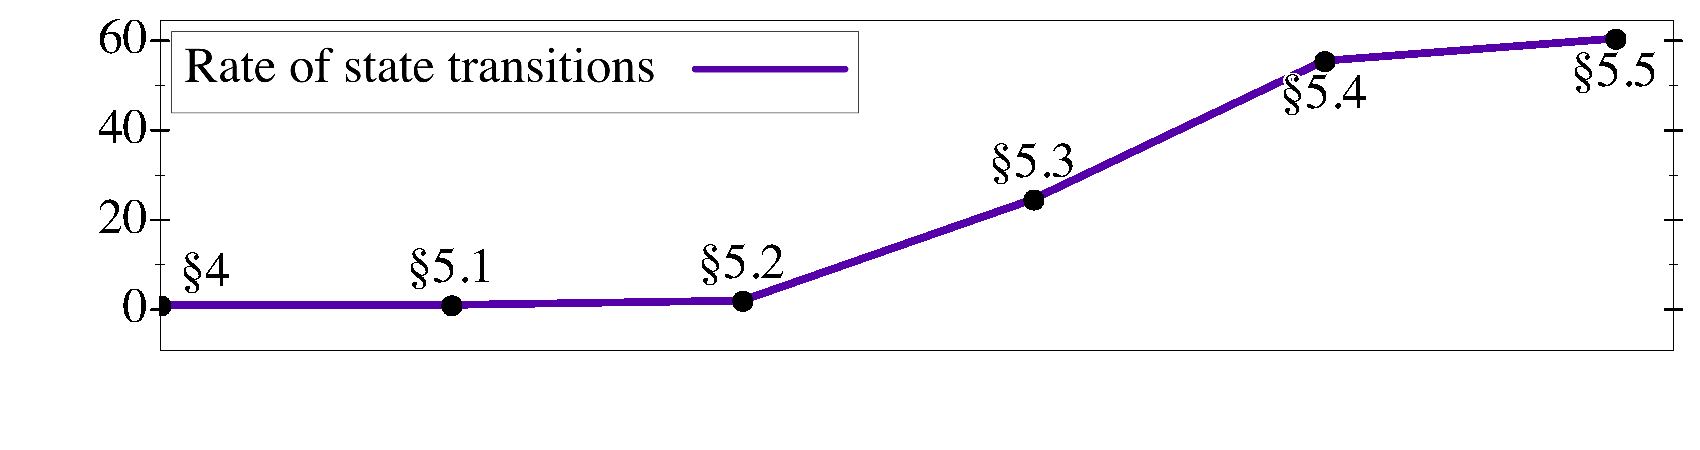
\includegraphics[width=3.2in]{church-relative-speed}
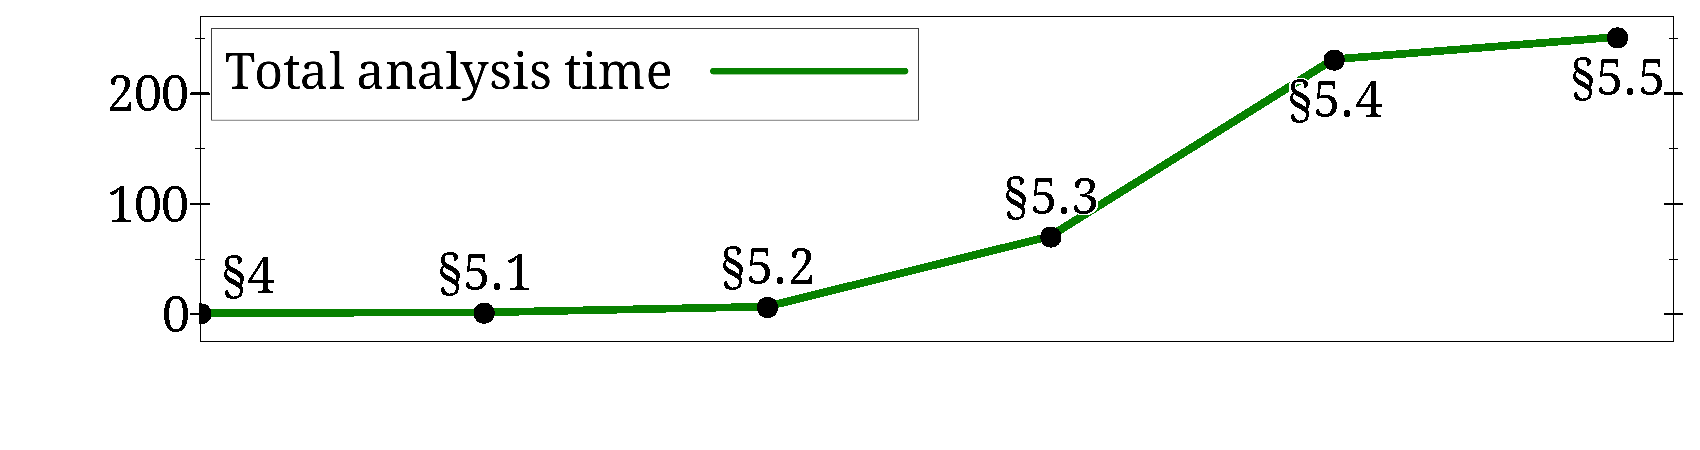
\includegraphics[width=3.2in]{church-relative-time}
\vspace{-1.5em}
\end{center}
\caption{Factor improvements over the baseline analyzer for the
  \Church{} benchmark in terms of peak memory usage, the rate of state
  transitions, and total analysis time. (Bigger is better.) Each point
  is marked with the section that introduces the optimization.}
\label{fig:churchtime}
\end{figure}


We start with a quick review of the AAM approach to develop an
analysis framework and then apply our step-by-step optimization
techniques in the simplified setting of a core functional language.
This allows us to explicate the optimizations with a minimal amount of
inessential technical overhead.  Following that, we scale this
approach up to an analyzer for a realistic untyped, higher-order
imperative language with a number of interesting features and then
measure improvements across a suite of benchmarks.

At each step during the initial presentation and development, we
evaluated the implementation on a set of benchmarks. The highlighted
benchmark in figure \ref{fig:churchtime} is from Vardoulakis and
Shivers~\cite{dvanhorn:Vardoulakis2011CFA2} that tests distributivity
of multiplication over addition on Church numerals.  For the
step-by-step development, this benchmark is particularly informative:
\begin{enumerate}
\item it can be written in most modern programming languages,
%
\item it was designed to stress an analyzer's ability to deal with
  complicated environment and control structure arising from the use
  of higher-order functions to encode arithmetic, and
%
\item its improvement is about median in the benchmark suite
  considered in section~\ref{sec:eval}, and thus it serves as a good
  sanity check for each of the optimization techniques considered.
\end{enumerate}

We start, in section~\ref{sec:aam}, by developing an abstract
interpreter according to the AAM approach.  In the initial
abstraction, each state carries a store (what is called per-state
store variance). The space of stores is exponential in size; without
further abstraction, the analysis is exponential and thus cannot
analyze the example in a reasonable amount of time.  In
section~\ref{sec:baseline}, we perform a further abstraction by
widening the store.  The resulting analyzer sacrifices precision for
speed and is able to analyze the example in about 1 minute.  This step
is described by Van Horn and Might~\cite[\S
3.5--6]{dvanhorn:VanHorn2012Systematic} and is necessary to make even
small examples feasible.  We therefore take a widened interpreter as
the baseline for our evaluation.

Section~\ref{sec:opt} gives a series of simple abstractions and
implementation techniques that, in total, speed up the analysis by
nearly a factor of 500, dropping the analysis time to a fraction of a
second.  Figure~\ref{fig:churchtime} shows the step-wise improvement
of the analysis time for this example.

\begin{figure}[t]
\begin{center}
\begin{tabular}{ccc}
\raisebox{1ex-\height}{
\includegraphics[height=3.5in]{introspective-base.pdf}}
&
\raisebox{1ex-\height}{
\includegraphics[height=3.5in]{introspective-lazy.pdf}}
&
\raisebox{1ex-\height}{
\includegraphics[height=3in]{introspective-lazyc.pdf}}
\\
(a) Baseline
&
(b) Lazy
&
(c) Compiled (\& lazy)
\end{tabular}
\end{center}
\caption{Example state graphs for the program above.  Part (a) shows
  the result of the baseline analyzer.  It has long ``corridor''
  transitions and ``diamond'' subgraphs that fan-out from
  nondeterminism and fan-in from joins.  Part (b) shows the result of
  performing nondeterminism lazily and thus avoids many of the diamond
  subgraphs.  Part (c) shows the result of abstract compilation that
  removes interpretive overhead in the form of intermediate states,
  thus minimizing the corridor transitions.  The end result is a more
  compact abstraction of the program that can be generated faster.}
\label{fig:state-graphs}
\end{figure}

The AAM approach, in essence, does the following: it takes a
machine-based view of computation and turns it into a \emph{finitary
  approximation} by bounding the size of the store.  With a limited
address space, the store must map addresses to \emph{sets} of values.
Store updates are interpreted as joins, and store dereferences are
interpreted by non-deterministic choice of an element from a set.  The
result of analyzing a program is a finite directed graph where nodes
in the graph are (abstract) machine states and edges denote machine
transitions between states.

The techniques we propose for optimizing analysis fall into the
following categories:
\begin{enumerate}
\item generate fewer states by avoiding the eager exploration of
  non-deterministic choices that will later collapse into a single
  join point.  We accomplish this by applying lazy evaluation
  techniques so that non-determinism is evaluated \emph{by need}.

\item generate fewer states by avoiding unnecessary, intermediate
  states of a computation.  We accomplish this by applying compilation
  techniques from functional languages to avoid interpretive overhead
  in the machine transition system.

\item generate states faster.  We accomplish this by better algorithm
  design in the fixed-point computation we use to generate state graphs.
\end{enumerate}
Figure~\ref{fig:state-graphs} shows the effect of (1) and (2) for a
small example due to Earl, et
al.~\cite{dvanhorn:Earl2012Introspective}.
By generating significantly fewer states at a significantly faster
rate, we are able to achieve large performance improvements in terms
of both time and space.

Section~\ref{sec:eval} describes the evaluation of each optimization
technique applied to an implementation supporting a more realistic set
of features, including mutation, first-class control, compound data, a
full numeric tower and many more forms of primitive data and
operations.
%
We evaluate this implementation against a set of benchmark programs
drawn from the literature.
%
For all benchmarks, the optimized analyzer outperforms the baseline
by at least a factor of
% 475
two to
% 4,382
three orders of magnitude.

Section~\ref{sec:related} relates this work to the literature and
section~\ref{sec:conclusion} concludes.

%\newpage
\section{Abstract interpretation of ISWIM}
\label{sec:aam}

In this section, we give a brief review of the AAM approach by
defining a sound analytic framework for a core higher-order functional
language: Landin's ISWIM~\cite{dvanhorn:Landin1966Next}.  In the
subsequent sections, we will explore optimizations for the analyzer in
this simplified setting, but scaling these techniques to realistic
languages is straightforward and has been done for the analyzer
evaluated in section~\ref{sec:eval}.

ISWIM is a family of programming languages parameterized by a set of
base values and operations.  To make things concrete, we consider a
member of the ISWIM family with integers, booleans, and a few
operations.
%
Figure~\ref{fig:syntax} defines the syntax of ISWIM.  It
includes variables, literals (either integers, booleans, or
operations), $\lambda$-expressions for defining procedures, procedure
applications, and conditionals.  Expressions carry a label, $\mlab$,
which is drawn from an unspecified set and denotes the source location
of the expression; labels are used to disambiguate distinct, but
syntactically identical pieces of syntax.  We omit the label
annotation in contexts where it is irrelevant.

\begin{figure}
\[
\begin{array}{l@{\qquad}rcl}
\text{Expressions} & \mexp &=& \svar[^\mlab]\mvar\\
&&|& \slit[^\mlab]\mlit\\
&&|& \slam[^\mlab]\mvar\mexp\\
&&|& \sapp[^\mlab]\mexp\mexp \\
&&|& \sif[^\mlab]\mexp\mexp\mexp \\
\text{Variables}&\mvar &=& \syntax{x}\ |\ \syntax{y}\ |\ \dots\\
\text{Literals}&\mlit &=& \mnum\ |\ \mbln\ |\ \mop\\
\text{Integers}&\mnum &=& \syntax{0}\ |\ \syntax{1}\ |\ \syntax{-1}\ |\ \dots\\
\text{Booleans}&\mbln &=& \strue\ |\ \sfalse\\
\text{Operations}&\mop &=& \syntax{zero?}\ |\ \syntax{add1}\ |\ \syntax{sub1}\ |\ \dots
\end{array}
\]
\caption{Syntax of ISWIM}
\label{fig:syntax}
\end{figure}

\begin{figure}
\[
\begin{array}{l@{\qquad}rcl}
\text{Values} & \mval,\mvalx{u} &=& \clos{\mvar,\mexp,\menv}\ |\ \mlit\ |\ \mkont\\
\text{States} & \mstate &=& \ev{\mexp,\menv,\msto,\mkont}\\
                       &&|& \co{\mkont,\mval,\msto}\\
                       &&|& \ap{\mval,\mval,\msto,\mkont}\\
\text{Continuations} & \mkont &=& \kmt\\
&&|& \kfn{\mval,\mkaddr}\\
&&|& \kar{\mexp,\menv,\mkaddr}\\
&&|& \kif{\mexp,\mexp,\menv,\mkaddr}\\
\text{Addresses} &\maddr&\in&\Addr \\
\text{Environments} &\menv&\in& \Var \rightharpoonup \Addr\\
\text{Stores} &\msto&\in& \Addr \rightharpoonup \mathcal{P}(\Value)
\end{array}
\]
\caption{Abstract machine components}
\label{fig:domains}
\end{figure}


The semantics are defined in terms of a machine model.  The machine
components are defined in figure~\ref{fig:domains};
figure~\ref{fig:aam} defines the transition relation.  The evaluation
of a program is defined as its set of traces that arise from iterating the
machine transition relation.  The
machine is a very slight variation on a standard abstract machine for
ISWIM in ``eval, continue, apply'' form~\cite{dvanhorn:Danvy:DSc}.  It
can be systematically derived from a definitional interpreter through
a continuation-passing style transformation and defunctionalization,
or from a structural operational semantics using the refocusing
construction of Danvy and
Nielsen~\cite{dvanhorn:Danvy-Nielsen:RS-04-26}.

Compared with the standard machine semantics, this definition is
different in the following ways, which make it abstractable as a
program analyzer:
\begin{itemize}
\item the store maps addresses to \emph{sets} of values,\footnote{
More generally, we can have stores map to any domain that forms
 a Galois connection with values, enabling $\interpdelta$ to
produce elaborate abstractions of base values (e.g., interval or octagon
abstractions). We use sets of values for a simpler exposition.
} not
  single values,

\item continuations are heap-allocated, not stack-allocated,
\item there are ``timestamps'' ($\mcntr \in \Counter$) and syntax
  labels ($\mlab$) threaded through the computation, and
\item the machine is implicitly parameterized by the functions
  $\alloc$, $\allockont$, $\tick$, $\interpdelta$, and spaces
  $\Addr$, $\Counter$ (and initial $\mcntr_0 \in \Counter$).
\end{itemize}


\begin{figure}
\begin{gather*}
\begin{align*}
\traces(\mexp) &= \{ \ev[^{\mtcntr}]{\mexp,\varnothing,\varnothing,\kmt} \multimachstep \mstate \} \text{ where }
\end{align*}
\\[2mm]
\begin{array}{@{}r@{\ }c@{\ }l@{}}
\mstate &\machstep&\mstate' \text{ defined to be the following} \\
&&\text{let } \mcntr' =\tick(\mstate) \\
%% EVAL
\ev{\svar\mvar,\menv,\msto,\mkont} &\machstep&
\co{\mkont,\mval,\msto}
\text{ if }\mval \in \msto(\menv(\mvar))
\\
\ev{\slit\mlit,\menv,\msto,\mkont} &\machstep&
\co{\mkont,\mlit,\msto}
\\
\ev[^\mcntr]{\slam\mvar\mexp,\menv,\msto,\mkont} &\machstep&
\co[^{\mcntr'}]{\mkont,\clos{\mvar,\mexp,\menv},\msto}
\\
\ev[^\mcntr]{\sapp[^\mlab]{\mexpi0}{\mexpi1},\menv,\msto,\mkont} &\machstep&
\ev[^{\mcntr'}]{\mexpi{0},\menv,\msto',\kar[_\mlab^\mcntr]{\mexpi{1},\menv,\mkaddr}}
\\
&&
\text{ where }\mkaddr = \allockont^\mcntr_\mlab(\msto,\mkont) \\
&&\phantom{\text{ where }}\msto' = \msto\sqcup[\mkaddr \mapsto \setof{\mkont}]
\\
\ev[^\mcntr]{\sif[^\mlab]{\mexpi0}{\mexpi1}{\mexpi2},\menv,\msto,\mkont} &\machstep&
\ev[^{\mcntr'}]{\mexpi0,\menv,\msto',\kif[^\mcntr]{\mexpi1,\mexpi2,\menv,\mkaddr}}
\\
&&
\text{ where }\mkaddr = \allockont^\mcntr_\mlab(\msto,\mkont) \\
&&\phantom{\text{ where }}\msto' = \msto\sqcup[\mkaddr \mapsto \setof{\mkont}]
\\[2mm]
%% CONTINUE
\co{\kmt,\mval,\msto} &\machstep&
\ans{\msto,\mval}
\\
\co{\kar[^\mcntr_\mlab]{\mexp,\menv,\mkaddr},\mval,\msto} & \machstep&
\ev[^\mcntr]{\mexp,\menv,\msto,\kfn[^\mcntr_\mlab]{\mval,\mkaddr}}
\\
\co{\kfn[^\mcntr_\mlab]{{\mvalx{u}},\mkaddr},\mval,\msto} & \machstep&
\ap[^\mcntr_\mlab]{\mvalx{u},\mval,\mkont,\msto}
\text{ if }\mkont \in \msto(\mkaddr)
\\
\co{\kif[^\mcntr]{\mexpi0,\mexpi1,\menv,\mkaddr},\strue,\msto} & \machstep&
\ev[^{\mcntr'}]{\mexpi0,\menv,\msto,\mkont}
\text{ if }\mkont\in\msto(\mkaddr)
\\
\co{\kif[^\mcntr]{\mexpi0,\mexpi1,\menv,\mkaddr},\sfalse,\msto} & \machstep&
\ev[^{\mcntr'}]{\mexpi1,\menv,\msto,\mkont}
\text{ if }\mkont\in\msto(\mkaddr)
\\[2mm]
%% APPLY
\ap[^\mcntr_\mlab]{\clos{\mvar,\mexp,\menv},\mval,\msto,\mkont} & \machstep&
\ev[^{\mcntr'}\!]{\mexp,\menv',\msto',\mkont}
\\
&&\text{ where } \maddr  =\alloc(\mstate) \\
&&\phantom{\text{ where }} \menv' = \menv[\mvar\mapsto\maddr] \\
&&\phantom{\text{ where }} \msto' = \msto\sqcup[\maddr\mapsto\{\mval\}] \\
\\
\ap[^\mcntr_\mlab]{\mop,\mval,\msto,\mkont} & \machstep&
\co{\mkont,\mval',\msto}
\text{ if } \mval'\in\interpdelta(\mop,\mval)
\end{array}
\end{gather*}
\caption{Abstract abstract machine for ISWIM}
\label{fig:aam}
\end{figure}


\paragraph{Concrete interpretation} To characterize concrete interpretation, set the implicit
parameters of the relation given in figure~\ref{fig:aam} as follows:
\begin{align*}
\alloc(\mstate) &= \maddr \mbox{ where } \maddr \notin \text{ the } \msto \text{ within } \mstate \\
\allockont^\mcntr_\mlab(\msto,\mkont) &=\mkaddr \mbox{ where } \mkaddr \notin \msto
\end{align*}
These functions appear to ignore $\mlab$ and $\mcntr$, but they can be
used to determinize the choice of fresh addresses. The $\sqcup$ on
stores in the figure is a point-wise lifting of $\cup$: $\msto \sqcup \msto' =
\lambda \maddr. \msto(\maddr) \cup \msto'(\maddr)$. The resulting
relation is non-deterministic in its choice of addresses, however it
must always choose a fresh address when allocating a continuation or
variable binding.  If we consider machine states equivalent up to
consistent renaming and fix an allocation scheme, this relation
defines a deterministic machine (the relation is really a function).

The interpretation of primitive operations is defined by setting
$\interpdelta$ as follows:
\begin{align*}
\mnum+1 &\in \interpdelta(\saddone,\mnum) &
\mnum-1 &\in \interpdelta(\ssubone,\mnum)\\
\strue &\in \interpdelta(\szerohuh,\szero) &
\sfalse &\in \interpdelta(\szerohuh,\mnum)\text{ if }\mnum\neq \szero\\
\end{align*}


\paragraph{Abstract interpretation} To characterize abstract
interpretation, set the implicit parameters just as above, but drop
the $\maddr \not\in \msto$ condition. The $\interpdelta$ relation takes some care
to not make the analysis run forever; a simple instantiation is a flat
abstraction where arithmetic operations return an abstract top element
$\sNum$, and $\szerohuh$ returns both $\strue$ and $\sfalse$ on
$\sNum$.  This family of interpreters is also non-deterministic in
choices of addresses, but it is free to choose addresses that are
already in use.  Consequently, the machines may be non-deterministic
when multiple values reside in a store location.

It is important to recognize from this definition that \emph{any}
allocation strategy is a sound abstract
interpretation~\cite{dvanhorn:Might2009Posteriori}.  In particular,
concrete interpretation is a kind of abstract interpretation.  So is
an interpretation that allocates a single cell into which all bindings
and continuations are stored.  The former is an abstract
interpretation that is non-computable and gives only the ground truth
of a programs behavior; the latter is an abstract interpretation
that is easy to compute but gives little information.  Useful program
analyses lay somewhere in between and can be characterized by their
choice of address representation and allocation strategy.  Uniform
\(k\)-CFA~\cite{dvanhorn:nielson-nielson-popl97}, presented next, is one such analysis.

\paragraph{Uniform \(k\)-CFA} To characterize uniform \(k\)-CFA, set the allocation
strategy as follows, for a fixed constant \(k\):

\begin{align*}
\Counter &= \Label^* \\
\mtcntr &= \epsilon \\
\alloc(\ev[^\mcntr]{\sapp[^\mlab]{\mexpi0}{\mexpi1},\menv,\msto,\mkont} &= \mlab\mcntr \\
\alloc(\ap[^\mcntr_\mlab]{\clos{\mvar,\mexp,\menv},\mval,\msto,\mkont}) &= \mvar\kpush[_k]{\mlab\mcntr} \\
\allockont^\mcntr_\mlab(\msto,\mkont) &= \mlab\mcntr \\
\tick(\ev[^\mcntr]{\mexp,\menv,\msto,\mkont}) &= \mcntr \\
\tick(\co{\kar[^\mcntr]{\mexp,\menv,\mkaddr},\mval,\msto}) &= \mcntr \\
\tick(\ap[^\mcntr_\mlab]{\mvalx{u},\mval,\mkont}) &= \kpush[_k]{\mlab\mcntr} \\
  \kpush[_0]{\mcntr} &= \kpush[_k]{\mtcntr} = \mtcntr \\
  \kpush[_{k+1}]{\mlab\mcntr} &= \mlab\kpush[_k]{\mcntr} \\
\end{align*}
The \(\lfloor\cdot\rfloor_k\) notation denotes the truncation of a list
of symbols to the leftmost \(k\) symbols.

All that remains is the interpretation of primitives.  For abstract
interpretation, we set $\interpdelta$ to the function that returns
$\sNum$ on all inputs---a symbolic value we interpret as denoting the
set of all integers.

At this point, we have abstracted the original machine to one which
has a finite state space for any given program, and thus forms the
basis of a sound, computable program analyzer for ISWIM.

\section{From machine semantics to baseline analyzer}
\label{sec:baseline}

The uniform $k$-CFA allocation strategy would make $\traces$ in figure
\ref{fig:aam} a computable abstraction of possible executions, but one
that is too inefficient to run, even on small examples.  Through this
section, we explain a succession of approximations to reach a more
appropriate baseline analysis.
%
We ground this path by first formulating the analysis in terms of a
classic fixed-point computation.


\subsection{Static analysis as fixed-point computation}
\label{sec:fixpoint}

Conceptually, the AAM approach calls for computing an analysis as a
graph exploration: (1) start with an initial state, and (2) compute
the transitive closure of the transition relation from that state. All
visited states are potentially reachable in the concrete, and all
paths through the graph are possible traces of execution.

We can cast this exploration process in terms of a fixed-point calculation.
%
Given the initial state $\mstate_0$ and the transition relation $\machstep$,
we define the global transfer function:
\begin{equation*}
 F_{\mstate_0} : \wp(\State) \times \wp(\State\times\State) \to \wp(\State) \times \wp(\State\times\State)\text.
\end{equation*}
Internally, this global transfer function computes the successors of all supplied states, and then includes the initial state:
\begin{align*}
  F_{\mstate_0}(V,E) &= (\{ \mstate_0 \} \cup V', E') \\
    E' &= \setof{ (\mstate,\mstate') \mid \mstate \in V \text{ and } \mstate \machstep \mstate'} \\
    V' &= \setof{ \mstate' \mid (\mstate,\mstate') \in E'}
\end{align*}
Then, the evaluator for the analysis computes the least fixed-point of the global transfer function:
\begin{equation*}
 \eval(\mexp) = \mathrm{lfp}(F_{\mstate_0})\text{,}
\end{equation*}
where $\mstate_0 = \ev[^\mtcntr]{\mexp, \varnothing, \varnothing, \kmt}$.

The possible traces of execution tell us the most about a program, so
we take $\traces(\mexp)$ to be the (regular) set of paths through the
computed graph. We elide the construction of the set of edges in this paper.

To conduct this \naive{} exploration on the \Church{} example would require
considerable time.  Even though the state space is finite, it is exponential in
the size of the program.  Even with $k = 0$, there are exponentially many
stores in the AAM framework.

In the next subsection, we fix this with store widening to reach polynomial
(albeit of high degree) complexity.
%
This widening effectively lifts the store out of individual states to create
a single, global shared store for all.


\subsection{Store widening}
\label{sec:storewiden}

A common technique to accelerate convergence in flow analyses is to share a
common, global store.
%
To retain soundness, this store grows monotonically.
%
Formally, we can cast this optimization as a second abstraction or as the
application of a widening operator during the fixed-point iteration.
%
In the ISWIM language, such a widening makes 0-CFA quartic in the size of the
program.
%
Thus, complexity drops from intractable exponentiality to a merely
daunting polynomial.

Since we can cast this optimization as a widening, there is no need to change
the transition relation itself.
%
Rather, what changes is the structure of the fixed-point iteration.
%
In each pass, the algorithm will collect all newly produced stores and join
them together.
%
Then, before each transition, it will install this joined store into current
state.

To describe this process, AAM defined a transformation of the reduction relation so that it operates on
a pair of a set of contexts ($C$) and a store ($\sigma$).
%
A context includes all non-store components, \emph{e.g.}, the expression, the environment and the stack.
%
The transformed relation, $\widehat{\machstep}$, is
%
\begin{align*}
(C, \msto) &\mathrel{\widehat{\machstep}} (C', \msto'), \\
\mbox{where } C' &= \{c' \mid \wn(c, \msto) \mathrel{\machstep} \wn(c', \msto^c), c \in C\} \\
              \msto' &= \bigsqcup\; \{\msto^c \mid \wn(c,\msto)\mathrel{\machstep} \wn(c', \msto^c), c \in C\} \\
\wn &: \widehat{\State} \times \Store \to \State \\
\wn(\ev{\mexp, \menv, \mkont}, \msto) &= \ev{\mexp, \menv, \msto, \mkont} \\
\wn(\co{\mval, \mkont}, \msto) &= \co{\mval, \mkont, \msto} \\
\wn(\ap{\mvalx{u}, \mval, \mkont}, \msto) &= \ap{\mvalx{u}, \mval, \msto, \mkont} \\
\wn(\ans{\mval}, \msto) &= \ans{\msto, \mval}
\end{align*}
%
In effect, the new store is computed as the least upper bound of all
stores after stepping. For clarity, we will exhibit non-widened
semantics unless a technique specifically requires it. The final step
to the baseline takes the complexity from quartic to cubic in the
monovariant case.

\subsection{Store-allocate all values}
\label{sec:baselineeval}

The final approximation we make to get to our baseline is to
store-allocate all values that appear, so that any non-machine state
that contains a value instead contains an address to a value.  The AAM
approach stops at the previous optimization.  However, the {\tt fn}
continuation stores a value, and this makes the space of continuations
quadratic rather than linear in the size of the program, for a
monovariant analysis like 0-CFA.  Having the space of continuations
grow linearly with the size of the program will drop the overall
complexity to cubic (as expected).

To achieve this linearity for continuations, we allocate an address
for the value position when we create the continuation.  This address
and the tail address are both determined by the label of the
application point, so the space becomes linear and the overall
complexity drops to cubic.  This is a critical abstraction in
languages with $n$-ary functions, since otherwise the continuation
space grows super-exponentially. We extend the semantics to
additionally allocate an address for the function value when creating
the $\kfn{}$ continuation. The continuation has to contain this address
to remember where to retreive values from in the store.

The new evaluation rules follow, where $\mcntr' = \tick(\mstate)$:
% In theory, this aggressive distinction between continuations might buy
% additional precision, but in practice, it does not.

\newcommand{\ext}[3]{#1\sqcup[#2\mapsto#3]}
%\newcommand{\ext}[3]{ext(#1,#2,#3)}

HERE

\begin{align*}
\co[^\mcntr]{\kar{\mexp,\menv,\mkaddr},\mval,\msto} & \machstep
\ev[^{\mcntr'}]{\mexp,\menv,\msto',\kfn{\maddr_f,\mkaddr}} \\
\text{ where }
  \maddr_f &= \alloc(\mstate) \\
  \msto' &= \ext{\msto}{\maddr_f}{\{\mval\}}
\end{align*}
Now instead of storing the evaluated function in the continuation
frame itself, we indirect it through the store for further control on
complexity and precision.

\begin{align*}
\co[^\mcntr]{\kfn{\maddr_f,\mkaddr},\mval,\msto} & \machstep
\ap[^{\mcntr'}_\mlab]{\mvalx{u},\mval,\mkont,\msto'}
\\
\text{ if } \mkont &\in \msto(\mkaddr), \mvalx{u} \in \msto(\maddr_f)
\end{align*}
Associated with this indirection, we now apply all functions stored in
the address. This nondeterminism is demanded in order to continue with
evaluation. More generally, this is because applied functions are in
\emph{strict position} (more about that later).

% This extra store-allocation is effectively naming all intermediate
% results, and thus the precision aligns with an analysis specialized to
% ANF. We can also play a representation trick in 0-CFA and remove
% $\menv$. In monovariant analyses, variables map to themselves, meaning
% $\menv$ is effectively the identity function. That degeneration, in
% turn, allows us to discard it from the analysis.

% Wide Store: cpu time: 551571 real time: 571319 gc time: 4003

\section{Implementation techniques}
\label{sec:opt}

In this section, we discuss the optimizations for abstract interpreters that
yield our ultimate performance gains.
%
We have two broad categories of these optimizations: (1) pragmatic
improvement, (2) transition elimination.
%
The pragmatic improvements reduce overhead and trade space for time
by utilizing:
\begin{enumerate}
 \item timestamped stores;
 \item store deltas; and
 \item imperative, preallocated data structures.
\end{enumerate}
The transition-elimination optimizations reduce the overall number of transitions
made by the analyzer by performing:
\begin{enumerate}
  \setcounter{enumi}{3}
 \item frontier-based semantics
 \item lazy non-determinism and
 \item abstract compilation;
\end{enumerate}

All pragmatic improvements are precision preserving (form complete
abstractions), but the semantic changes are not in some cases, for reasons we
will describe. We did not observe the precision differences in our evaluation.

We apply the frontier-based semantics combined with timestamped stores
as our first step.  The move to the imperative will be made last in
order to show the effectiveness of these techniques in the purely
functional realm.

\subsection{Timestamped frontier}

The semantics given for store widening in section \ref{sec:storewiden},
while simple, is wasteful. It also does not model what typical
implementations do. It causes all states found so far to step each
iteration, even if they are not revisited. This has negative
performance \emph{and} precision consequences (changes to the store
can travel back in time in straight-line code). We instead use a
frontier-based semantics that corresponds to the classic ``worklist''
algorithms for analysis. The difference is that the store is not
modified in-place, but updated after all frontier states have been
processed. This has implications for the analysis' precision and
determinism. Specifically, higher precision, and it is deterministic
even if set iteration is not.

\begin{align*}
(S, F, \msto) &\mathrel{\widehat{\machstep}} (S \cup S', F', \msto') \\
\mbox{where } I &= \{(c',\msto^c) \mid \wn(c, \msto) \mathrel{\machstep} \wn(c', \msto^c), c \in F\} \\
              \msto' &= \bigsqcup\; \{\msto^c \mid (\_,\msto^c) \in I\} \\
              F' &= \{c \mid (c,\_) \in I, (c,\msto') \notin S\} \\
              S' &= \setof{(c,\msto') \mid c \in F'} \\
\inject(e) &= (\setof{\ttuple{c_0}{\bot}},\setof{c_0},\bot) \\
\text{ where } c_0 &= \ev{e,\bot,\kmt}
\end{align*}

Notice that now $S$ has several copies of the abstract store in it. As
it is, this semantics is much less efficient (but still more precise)
than the previously proposed semantics because membership checks have
to compare entire stores. Checking equality is expensive because the stores within each are
large, and every entry must be checked against every other. Hashes can
sometimes rule out inequality relatively quickly, but the incidence of
collisions and actual equality is costly.

And, there is a better way. Shivers' original work on $k$-CFA was
susceptible to the same problem, and he suggested three complementary
optimizations: (1) make the store global; (2) update the store
imperatively; and (3) associate every change in the store with a
version number -- its timestamp. Then, put timestamps in states
where previously there were stores. Given two states, the analysis can
now compare their stores just by comparing their timestamps -- a
constant-time operation.

There are two subtle losses of precision in Shivers' original
timestamp technique that we can fix.

\begin{enumerate}
\item{In our semantics, the store does not change until the entire
    frontier has been explored. This avoids cross-branch pollution
    which would not otherwise happen, e.g., when one branch writes to
    address $\maddr$ and another branch reads from address
    $\maddr$.}
\item{The common implementation strategy for timestamps destructively
    updates each state's timestamp. This loses \emph{temporal}
    information about the contexts a state is visited in, and in what
    order. The semantics is different - we can't precisely answer
    questions about the traces of the reduction relation we defined.
    Our semantics has a drop-in replacement of timestamps for stores
    in the seen set ($S$), so we do not experience precision loss.}
\end{enumerate}

\begin{align*}
\Sigma &\in \Store^* \\
S &\subseteq {\mathbb N} \times \widehat{\State} \\
F &\subseteq \widehat{\State} \\
(S, F, \msto, \Sigma, t) &\mathrel{\widehat{\machstep}^T} (S \cup S', F', \msto', \Sigma', t') \\
\mbox{where } I &= \setof{(c',\msto^c) \mid \wn(c, \msto) \mathrel{\machstep} \wn(c', \msto^c), c \in F} \\
              \msto' &= \bigsqcup\; \{\msto^c \mid (\_,\msto^c) \in I\} \\
              (t',\Sigma') &=\left\{\begin{array}{ll}
                           (t+1,\msto'\Sigma') & \text{ if } \msto' \neq \msto \\
                           (t,\Sigma)   & \text{ otherwise}
                          \end{array}\right. \\
              F' &= \setof{c \mid (c,\_) \in I, (c,t') \notin S} \\
              S' &= \setof{(c,t') \mid c \in F'}\\
\inject(e) &= (\setof{\ttuple{c_0}{0}},\setof{c_0},\bot,\cons{\bot}{\epsilon},0) \\
\text{ where } c_0 &= \ev{e,\bot,\kmt}
\end{align*}

The observation Shivers made was that the store is increasing
monotonically, so all stores throughout execution will be totally
ordered (form a chain). This observation allows you to replace stores
with pointers into this chain. We keep the stores around in $\Sigma$
to acheive a complete abstraction. This corresponds to the temporal
information about the execution's effect on the store.

Note also that $F$ is only populated with states that have not been
seen at the resulting store. This is what produces the more precise
abstraction than the baseline widening.

The general fixed-point combinator we showed above can be specialized
to this semantics, as well. In fact, $\widehat{\machstep}^T$ is a functional
relation, so we can get the least fixed-point of it directly.

\begin{lemma}
  $\widehat{\machstep}$ maintains the invariant that all stores in $S$ are
  totally ordered and $\msto$ is an upper bound of the stores in $S$.
\end{lemma}

\begin{lemma}
  $\widehat{\machstep}^T$ maintains the invariant that $\Sigma$ is in
  order with respect to $\sqsupset$ and $\msto = \hd(\Sigma)$.
\end{lemma}

\begin{theorem}
Timestamps are a complete abstraction
\end{theorem}
The proof follows from the galois connection that, in one direction,
sorts all the stores in $S$ to form $\Sigma$, and translates stores in
$S$ to their distance from the end of $\Sigma$. In the other
direction, timestamps are replaced by the stores they point to.

\subsection{Locally log-based store deltas}

The above technique requires joining entire (large) stores
together. Additionally, there is still a comparison of stores, which
we established is expensive. Not every step will modify all addresses
of the store, so joining entire stores is wasteful in terms of memory
and time. We can instead log store changes and replay the change log
on the full store after all steps have completed, noting when there is
an actual change. This uses far fewer join and comparison operations,
leading to less overhead, and is precision-preserving.

We represent change logs as $\msdiff \in \StoreDelta = (\Addr \times
  \Set(\Storeable))^*$. Each $\msto\sqcup[\maddr \mapsto \mval{s}]$
 becomes a log addition
$\cons{\ttuple{\maddr}{\mval{s}}}{\msdiff}$, where $\msdiff$ begins
empty ($\mtlst$) for each step. Applying the changes to the full store
is straightforward:
\begin{equation*}
\replay : (\StoreDelta \times \Store) \to (\Store \times \Boolean)
\end{equation*}
\begin{align*}
\replay(\left[ \ttuple{\maddr_i}{\mval{s_i}}, \ldots\right], \msto) &=
\ttuple{\msto'}
       {\mval{s_i} \overset{?}{=} \msto'(\maddr_i) \vee \ldots} \\
\text{ where } \msto' &= {\msto \sqcup [\maddr_i \mapsto \mval{s_i}] \sqcup \ldots}
\end{align*}

We change the semantics slightly to add to the change log rather than
produce an entire modified store.  The transition relation is
identical except for the addition of this change log.  We maintain the
invariant that lookups will never rely on the change log, so we can
use the originally supplied store unmodified.

A taste of the changes to the reduction relation is as follows:

\begin{align*}
\dmachstep &\subseteq (\widehat{\State}\times\Store) \times (\widehat{\State}\times\StoreDelta) \\
\ttuple{\ap[^\mcntr_\mlab]{\clos{\mvar,\mexp,\menv},\mval,\mkont}}{\msto} & \dmachstep
\ttuple{\ev[^{\mcntr'}]{\mexp,\menv',\mkont}}{\cons{\ttuple{\maddr}{\setof{\mval}}}{\epsilon}} \\
\text{ where }\maddr &= \alloc(\mstate) \\
              \menv' &= \menv[\mvar\mapsto\maddr]
\end{align*}

% Compilation changes to additionally take a $\msdiff$ component, so the
% above rule's right hand side would instead be $k^{\mcntr'}(\menv',
% \msto, \msdiff', \mkont)$ where $k = \compile{e}$ would be in the closure.

We lift $\dmachstep$ to accommodate for the asymmetry
in the input and output, and change the frontier-based semantics in the following way:

\begin{align*}
(S, F, \msto,\Sigma,t) &\mathrel{\damachstep} (S \cup S', F', \msto',\Sigma',t') \\
\mbox{ where }
 I &= \setof{(\mastate',\msdiff) \mid \ttuple{\mastate}{\msto} \dmachstep \ttuple{\mastate'}{\msdiff} } \\
 \ttuple{\msto'}{\changep} &= \replay(\appendall(\setof{\msdiff \mid (\_,\msdiff) \in I}),\msto) \\
 \ttuple{t'}{\Sigma'} &=
     \left\{
       \begin{array}{ll}
         \ttuple{t+1}{\msto\Sigma} & \text{ if } \changep \\
         \ttuple{t}{\Sigma} & \text{ otherwise}
       \end{array}\right. \\
 F' &= \setof{\mastate \mid (\mastate,\_) \in I, (\mastate,t') \notin S} \\
 S' &= \setof{(\mastate,t') \mid c \in F'} \\
\appendall(\varnothing) &= \epsilon \\
\appendall(\setof{\msdiff}\cup\Xi) &= \append(\msdiff,\appendall(\Xi))
\end{align*}

Here $\appendall$ combines change logs across all non-deterministic
steps for a state to later be replayed. The order the combination
happens in doesn't matter, because join is associative and
commutative.

\begin{lemma}
$\ttuple{\mastate}{\msto} \dmachstep \ttuple{\mastate'}{\msdiff}$ iff
$\wn(\mastate,\msto) \machstep \wn(\mastate',\replay(\msdiff,\msto))$
\end{lemma}
By cases on $\dmachstep$ and $\machstep$.

\begin{lemma}[$\changep$ means change]
Let $\replay(\msdiff,\msto) = \ttuple{\msto'}{\changep}$. $\msto' \neq \msto$ iff $\changep$.
\end{lemma}
By induction on $\msdiff$.

\begin{theorem}
$\damachstep$ is a complete abstraction of $\widehat{\machstep}^T$.
\end{theorem}
Follows from previous lemma and that join is associative and commutative.

% Correctness here requires a lemma that relates the differences in the compilation functions.

% \begin{lemma}[Compile coherence]
% Let $\dcompile{\mexp}^\mcntr(\menv,\msto,\msdiff,\mkont) = \ttuple{\mastate}{\msdiff'}$
% and $\compile{\mexp}^\mcntr(\menv,\msto^*,\mkont^*) = \wn(\mastate',\msto^{*'})$.
% If $\msto \equiv \msto^*$, $\msdiff \equiv \msdiff^*$, and $\mkont \equiv \mkont^*$, then
% $\mastate' \equiv \mastate$
% and there exists an $\msdiff''$ such that \\
%    $\replay(\msdiff'',\replay(\msdiff^*,\msto^*)) \equiv \replay(\msdiff',\msto)$.
% \end{lemma}
% Here $\equiv$ means structurally the same, only compiled expressions
% are compiled with the updated compilation function that builds store
% deltas. Proof is by induction on $\mexp$.

% \begin{theorem}[Equivalence with wide abstract compilation]
% If $S \equiv S^*, F \equiv F^*, \msto \equiv \msto^*$, then
% $(S,F,\msto) \machstep (S',F',\msto')$ iff
% $\exists S^*_1, F^*_1, \msto^*_1.
%   S' \equiv S^*_1 \wedge F' \equiv F^*_1 \wedge \msto' \equiv \msto^*_1 \wedge
%   (S^*,F^*,\msto^*) \dmachstep (S^*_1,F^*_1,\msto^*_1)$
% \end{theorem}
% Proof by the above lemma and that replaying in any order is equivalent
% (associativity and commutativity of $\sqcup$).


\subsection{Lazy non-determinism}

Tracing the execution of the analysis reveals an immediate shortcoming:
there is a high degree of branching and merging in the exploration.
%
Surveying this branching has no benefit for precision.
%
For example, in a function application, {\tt (f x y)},
where {\tt f}, {\tt x} and {\tt y} each have several values
each argument evaluation induces $n$-way branching, only to be ultimately joined back together in their respective
application positions.
%
Transition patterns of this shape litter the state-graph:
%
\begin{center}
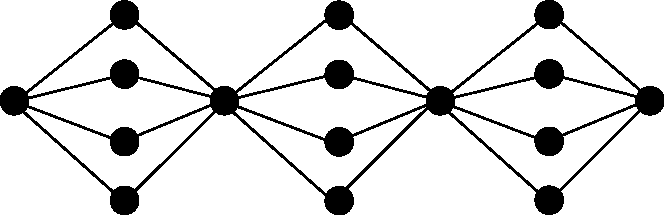
\includegraphics[scale=0.3]{fanout}
\end{center}
To avoid the spurious forking and joining, we {\it delay} the non-determinism
until and unless it is needed in {\it strict contexts} (such as the guard for an
{\tt if}, a called procedure, or a numerical primitive application).
%
Doing so collapses these forks and joins into a linear sequence of states:
\begin{center}

\includegraphics[scale=0.3]{lazy}
\end{center}

This shift does not change the concrete semantics of the language to
be lazy.  Rather, it abstracts over transitions that the original
non-deterministic semantics steps through.
%
We say the abstraction is \emph{lazy} because it delays splitting on
the values in an address until they are \emph{needed} in the
semantics. It does not change the execution order that leads to the
values that are stored in the address.

We introduce a new kind of value,
\spchoice
{$\saddr{\maddr}$}
{$\superposition{\mval{s}}$ (for ``superposition'')},
%
that represents a delayed non-deterministic choice of a value from
\spchoice
{$\msto(\maddr)$}
{$\mval{s}$}.
%
The following rules highlight the changes to the semantics:

\renewcommand{\ext}{\mathit{ext}}

\begin{align*}
\spchoice
{\force &: \Store \times \Value \to \Set(\Value) \\
 \force(\msto,\saddr{\maddr}) &= \msto(\maddr) \\
 \force(\msto,\mval) &= \setof{\mval}}
{\force &: \Value \to \Set(\Value) \\
 \force(\superposition{\mval{s}}) &= \mval{s} \\
 \force(\mval) &= \{\mval\}}
\\
%
\ev{\svar{\mvar},\menv,\mkont,\msto} &\lmachstep\;
\spchoice
{\co{\mkont,\saddr{\menv(\mvar)},\msto}}
{\co{\mkont,\superposition{\msto(\menv(\mvar))},\msto}} \\
%
\co{\kar[^\mcntr_\mlab]{\mexp,\menv,\mkaddr},\mval,\msto}
&\lmachstep\;
\ev[^{\mcntr'}]{\mexp,\menv,\msto',\kfn[^\mcntr_\mlab]{\maddr_f,\mkaddr}} \\
\text{ where }
\maddr_f &= \alloc(\mstate) \\
\msto' &=
\spchoice
{\msto \sqcup[\maddr \mapsto \force(\msto,\mval)]}
{\msto \sqcup[\maddr \mapsto \force(\mval)]} \\
%
\co{\kif[^\mcntr]{\mexpi0,\mexpi1,\menv,\mkaddr},\mval,\msto}
&\lmachstep\;
\ev[^{\mcntr'}]{\mexpi,\menv,\msto,\mkont} \\
\text{ if } \mkont &\in \msto(\mkaddr),
            \strue \in \spchoice{\force(\msto,\mval)}{\force(\mval)}
\end{align*}
Since {\tt if} guards are in strict position, we must force the value
to determine which branch to to take. The middle rule uses $\force$
only to combine with values in the store - it does not introduce
needless non-determinism.

\spchoice{
\noindent
We have two choices for how to implement lazy non-determinism.

\paragraph{Option 1: Lose precision; simplify implementation}
This semantics introduces a subtle precision difference over the
baseline. Consider a configuration where a reference to a variable and
a binding of a variable will happen in one step, since store widening
leads to stepping several states in one big ``step.'' With laziness,
the reference will mean the original binding(s) of the variable or the
new binding, because the actual store lookup is delayed one step
(i.e. laziness is administrative). Without laziness, the reference
will fan out to all the bindings of the variable before the new
binding happens and thus theoretically has an observable precision
difference. % All our benchmarks maintain their precision with lazy non-determinism, however.

\paragraph{Option 2: Regain precision; complicate implementation}
The administrative nature of laziness means that we could remove the
loss in precision by duplicating the reduction relation to specialize
variable lookup. This works since in the semantics of ISWIM with
store-allocated results consumes the value component of states in one
step. This is not the case for semantics that replicate the value
component across reductions, say for popping off exception handler
frames. Further convolution is needed to remove the administrative
nature of laziness in these semantics. Due to the increase of
conceptual and implementation complexity for negligible benefit, we
decided against this approach.

\paragraph{Our choice: option 1}
The configurations that lead to precision loss happen too rarely to
warrant the significant increase in time and memory needed for this
eager non-determinism. Indeed, were the variable reference a step
later and another binding not made in that step, the results of the
two approaches are the same. Without a widened store, lazy
non-determinism is not a complete abstraction with either approach,
but the precision gains are not immediately apparent due to fake
rebinding (a second reference to the same variable chooses a different
value from the first) and other problems. The performance and memory
gains are apparent, so we favor the simplicity over invisible
gains.}{}

\spchoice
{
\begin{theorem}[Soundness]
  If $\mstate \machstep \mstate'$ and $\mstate \sqsubseteq
  \mastate$ then there exists a $\mastate'$ such that $\mastate
  \lmachstep \mastate'$ and $\mstate' \sqsubseteq \mastate'$
\end{theorem}
Here $\sqsubseteq$ is straightforward - the LHS store must be
contained in the RHS store, and if values occur in the states, forcing
the LHS value must be a subset of forcing the corresponding RHS value.
The proof is by cases on $\mstate \machstep \mstate'$.}
{
\begin{theorem}[Completeness]For all $\mexp$,
 $\traces_{\text{Lazy}}(\mexp)$ is a complete abstraction of $\traces_{\text{ISWIM}}(\mexp)$.
\end{theorem}
We have a statement about traces because we need induction to show no
cruft values are in superposition.  The induction hypothesis tells us
that there are non-lazy traces that lead to all the values in
superposition, so when we take a lazy step, we are taking several
non-lazy steps, and we stay in sync. The other direction we just
collapse the superposition in each possibility to construct the
non-lazy traces.}

% Lazy:  cpu time: 32481 real time: 32881 gc time: 547

\subsection{Abstract compilation}

The prior optimization saved time by doing the same amount of
reasoning as before but in fewer transitions. We can exploit the same
idea---same reasoning, fewer transitions---with abstract
compilation. Abstract compilation transforms complex expressions whose
\emph{abstract} evaluation is deterministic into ``abstract
bytecodes.''  The abstract interpreter then does in one transition
what previously took many. In short, abstract compilation eliminates
unnecessary allocation, deallocation and branching. The technique is
precision preserving without store widening. We discuss the precision
differences with store widening at the end of the section.

The following example illustrates
the essence of abstract compilation effect:
\[
\mexp := \sapp{\sapp{\sapp\mvar{\mexp_1}}{\mexp_2}}{\mexp_3}
\]
makes the following transitions:
\begin{align}
& \ev[^\mcntr]{\sapp{\sapp{\sapp\mvar{\mexp_1}}{\mexp_2}}{\mexp_3},\menv,\msto_0,\mkont}\\
\machstep\; &
\ev[^{\mcntr'}]{\sapp{\sapp\mvar{\mexp_1}}{\mexp_2},\menv,\msto_1,\kar{\mexp_3,\menv,\maddr_1}}
\\
\machstep\; &
\ev[^{\mcntr''}]{\sapp\mvar{\mexp_1},\menv,\msto_2,\kar{\mexp_2,\menv,\maddr_2}}
\\
\machstep\; &
\ev[^{\mcntr'''}]{\mvar, \menv,\msto_3,\kar{\mexp_1,\menv,\maddr_3}} % {\mexp_2}
\\
\machstep\; &
\spchoice
{\co{\kar{\mexp_1,\menv,\maddr_3},\saddr{\menv(\mvar)},\msto_4}}
{\co{\kar{\mexp_1,\menv,\maddr_{f3},\maddr_{a3},\maddr_3},\superposition{\msto_4(\menv(\mvar))},\msto_4}}
\end{align}
where \(
\msto_4 = \msto_0 \sqcup [\maddr_1 \mapsto \setof{\mkont},
\maddr_2 \mapsto \setof{\kar{\compile{\mexp_3},\menv,\maddr_1}},
\maddr_3 \mapsto \setof{\kar{\compile{\mexp_2},\menv,\maddr_2}}]\).

Whereas abstract compilation gives us in one step:
\begin{align*}
\compile{\mexp}^\mcntr(\msto_0)(\menv,\epsilon,\mkont) =
\spchoice
{\co{\kar{\compile{\mexp_1},\menv,\maddr_3},\saddr{\menv(\mvar)}},\msdiff_4}
{\co{\kar{\compile{\mexp_1},\menv,\maddr_{f3},\maddr_{a3},\maddr_3},\superposition{\msto'_4(\menv(\mvar))},\msto'_4}}
\end{align*}
where
\begin{equation*}
\msdiff_4 = [\ttuple{\maddr_1}{\setof{\mkont}},
             \ttuple{\maddr_2}{\setof{\kar{\compile{\mexp_3},\menv,\maddr_1}}},
             \ttuple{\maddr_3}{\setof{\kar{\compile{\mexp_2},\menv,\maddr_2}}}]\text.
\end{equation*}

The compilation step converts expressions into functions that expect
the other components of the {\tt ev} state. Its definition in figure
\ref{fig:compile} shows close similarity to the rules for interpreting
{\tt ev} states. The next step is to change reduction rules that
create {\tt ev} states to instead call these functions. Figure
\ref{fig:caam} shows the modified reduction relation. The only change
from the previous semantics is that $\ev{}$ state construction is
replaced by calling the compiled expression. For notational coherence,
we write $\lambda^\mcntr(\mathit{args} \ldots)$ for
$\lambda(\mathit{args} \ldots, \mcntr)$ and
$\mcomp^\mcntr(\mathit{args}\ldots)$ for $\mcomp(\mathit{args}\ldots,
\mcntr)$.

\begin{figure}
\begin{align*}
\compile{\_} &: \Expr \to \Store \\
             &\phantom{: \Expr } \to \Env  \times \StoreDelta \times \Kont \times \Counter \\
             &\phantom{: \Expr } \to \State \\
\mcntr' &= \tick(\mlab,\menv,\msto,\mcntr) \\
\compile{\svar\mvar}_\msto &=
 \lambda^\mcntr(\menv,\msdiff,\mkont) .
\spchoice
{\co{\mkont,\saddr{\menv(\mvar)}},\msdiff}
{\co{\mkont,\superposition{\msto(\menv(\mvar))}},\msdiff}
\\
\compile{\slit\mlit}_\msto &= \lambda^\mcntr(\menv,\msdiff,\mkont) .
\co{\mkont,\mlit},\msdiff
\\
\compile{\slam\mvar\mexp}_\msto &= \lambda^\mcntr(\menv,\msdiff,\mkont) .
\co{\mkont,\clos{\mvar,\compile{\mexp},\menv}},\msdiff
\\
\compile{\sapp[^\mlab]{\mexpi0}{\mexpi1}}_\msto &= \lambda^\mcntr(\menv,\msdiff,\mkont) .
\compile{\mexpi0}^{\mcntr'}(\menv,\msdiff',\kar[_\mlab^\mcntr]{\compile{\mexpi1},\menv,\mkaddr})
\\
&\setlength\arraycolsep{5pt}
\begin{array}{lrl}
\text{ where } & \mkaddr = \allockont^\mcntr_\mlab(\msto,\mkont) \\
               & \msdiff' = \cons{\ttuple{\mkaddr}{\setof{\mkont}}}{\msdiff}
\end{array}
\\
\compile{\sif[^\mlab]{\mexpi0}{\mexpi1}{\mexpi2}}_\msto &= \lambda^\mcntr(\menv,\msdiff,\mkont) .
\compile{\mexpi0}^{\mcntr'}(\menv,\msdiff',\kif[^\mcntr]{\compile{\mexpi1},\compile{\mexpi2},\menv,\maddr})
\\
&\text{ where }\mkaddr = \allockont^\mcntr_\mlab(\msto,\mkont) \\
&\phantom{\text{ where }} \msdiff' = \cons{\ttuple{\mkaddr}{\setof{\mkont}}}{\msdiff}
\end{align*}
\caption{Abstract compilation}
\label{fig:compile}
\end{figure}

\begin{figure}
\begin{gather*}
\begin{align*}
\traces(\mexp) &= \setof{ \inject(\compile{\mexp}^\mtcntr_\bot(\bot,\epsilon,\kmt)) \multimachstep \mstate}
                    \text{ where } \\
\inject(\mastate,\msdiff) &= \wn(\mastate,\replay(\msdiff,\bot)) \\
\wn(\mastate,\msto) \machstep \wn(\mastate',\msto') &\iff \mastate \cmachstep_\msto \mastate',\msdiff \\
\msdiff \text{ is such that } &\replay(\msdiff,\msto) = \msto'
\end{align*}
\\[2mm]
\begin{align*}
%% CONTINUE
\co{\kmt,\mval} &\cmachstep_\msto
\ans{\mval'},\epsilon \text{ if } \mval' \in \spchoice{\force(\msto,\mval)}{\force(\mval)}
\\
\co{\kar[^\mcntr_\mlab]{\mcomp,\menv,\mkaddr},\mval} & \cmachstep_\msto
\mcomp^\mcntr(\msto)(\menv,\msdiff,\kfn[^\mcntr_\mlab]{\maddr_f,\mkaddr}) \\
\text{ where } \maddr_f &= \alloc(\mstate) \\
               \msdiff &= \cons{\ttuple{\maddr_f}{\force(\msto,\mval)}}{\epsilon}
\\
\co{\kfn[^\mcntr_\mlab]{\maddr_f,\mkaddr},\mval} & \cmachstep_\msto
\ap[^\mcntr_\mlab]{\mval,\mval\mkont},\epsilon \\
\text{ if }\mval &\in \msto(\maddr_f), \mkont \in \msto(\mkaddr)
\\
\co{\kif[^\mcntr]{\mcompi0,\mcompi1,\menv,\maddr},\strue} & \cmachstep_\msto
\mcompi{0}^\mcntr(\msto)(\menv,\epsilon,\mkont)
\text{ if }\mkont\in\msto(\maddr)
\\
\co{\kif[^\mcntr]{\mcompi0,\mcompi1,\menv,\maddr},\sfalse} & \cmachstep_\msto
\mcompi{1}^\mcntr(\msto)(\menv,\epsilon,\mkont)
\text{ if }\mkont\in\msto(\maddr)
\\[2mm]
%% APPLY
\ap[^\mcntr_\mlab]{\clos{\mvar,\mcomp,\menv},\mval,\mkont} & \cmachstep_\msto
\mcomp^{\mcntr'}(\msto)(\menv',\msdiff,\mkont) \\
\text{ where }\menv' &= \menv[\mvar\mapsto\maddr] \\
              \msdiff &= \cons{\ttuple{\maddr}{\force(\msto,\mval)}}{\epsilon}
\\
\ap{\mop,\mval,\mkont} & \cmachstep_\msto
\co{\mkont,\mval'},\epsilon \\
\text{ where } \mvalx{u} &\in \spchoice{\force(\msto,\mval)}{\force(\mval)}, \mval'\in\interpdelta(\mop,\mvalx{u})
\end{align*}
\end{gather*}
\caption{Abstract abstract machine for compiled ISWIM}
\label{fig:caam}
\end{figure}

\paragraph{Correctness}
The correctness of abstract compilation seems obvious, but it has
never before been rigorously proved. What constitutes correctness in
the case of dropped states, anyway? Applying an abstract bytecode's
function does many ``steps'' in one go, at the end of which, the two
semantics line up again (modulo representation of expressions). This
constitutes the use of a notion of stuttering. We provide a formal
analysis of abstract compilation \emph{without} store widening with a proof
of a stuttering bisimulation~\cite{ianjohnson:BCG88} between this
semantics and lazy non-determinism without widening to show precision
preservation. %We revisit store widening at the end of the section.

The number of transitions that can occur in succession from an
abstract bytecode is roughly bounded by the amount of expression
nesting in the program. The partial order that defines subexpressions
smaller than the expression in which they occur is well-founded, so we
use this observation to drive our use of a well-founded equivalence
bisimulation (WEB)~\cite{ianjohnson:manolios-diss}. WEBs are equivalent to the notion of a stuttering
bisimulation, but are more amenable to mechanisation (and thus
rigorous proof). They also only require reasoning over one step of the
reduction relation, which makes the proof concise.

We define a refinement from non-compiled to compiled states by
``committing'' all the actions of an $\ev{}$ state (defined similarly to
$\compile{\_}$, but immediately applies the functions), and
subsequently changing all expressions with their compiled
variants. Since WEBs are for single transition systems, a WEB
refinement is over the disjoint union of our two semantics, and the
equivalence relation we use is just that a state is related to its
refined state (and itself). Call this relation $B$.

Before we prove this setup is indeed a WEB, we need one lemma that
applying an abstract bytecode's function is equal to refining the
corresponding $\ev{}$ state:
%
\begin{lemma}[Compile/commit]
Let $\mastate,\msdiff' = \compile{\mexp}^\mcntr_{r(\msto)}(\menv,\msdiff,r(\mkont))$.
Let $\wn(\mastate',\msto') = r(\ev[^\mcntr]{\mexp,\menv,\msto,\mkont})$.
$\wn(\mastate,\replay(\msdiff',\msto)) = \wn(\mastate',\replay(\msdiff,\msto'))$.
\end{lemma}
The proof is by induction on $\mexp$.

\begin{theorem}[Precision preservation]
$B$ is a WEB on $\lmachstep \uplus \machstep$
\end{theorem}

The proof follows by cases on $\lmachstep \uplus \machstep$ with the
WEB \emph{witness} being the well-order on expressions (with a $\bot$
element), and the following $\erankt$, $\erankl$ functions:

\begin{align*}
\erankt(\ev[^\mcntr]{\mexp,\menv,\msto,\mkont}) &= \mexp \\
\erankt(\mstate) &= \bot \quad \text{otherwise} \\
\erankl(s,s') &= 0
\end{align*}
All cases are either simple steps or appeals to the well-order on $\erankt$'s range. The other rank function,
$\erankl$ is unnecessary, so we just make it the constant 0
function. The $\cmachstep$ cases are trivial.

\paragraph{Wide store and abstract compilation}
The fact that many changes happen in one step also makes the
comparison with the widened lazy semantics more subtle. It is possible
for different stores to occur between the different semantics because
abstract compilation can change the order in which the store is
changed. Consider the case where before we might call the same
function from two different places in 3 and 2 steps respectively,
compilation can make that 2 and 1, reversing the order that we bind
values in the store, leading to a mismatch from the previous
semantics. This kind of cross-step store poisoning is inevitable when
a store is shared between several traces. The binding could have just
as easily been observed the other way around in the non-compiled
semantics. Call $\camachstep$ the result of the widening operator from
the previous section on $\cmachstep$.

% Compile: cpu time: 255397 real time: 261532 gc time: 2947

% \noindent
% Compile + Lazy: cpu time: 31173 real time: 31642 gc time: 739

%\newpage

%% Delta Store +k Compile + Lazy:
%%    cpu time: 668 real time: 686 gc time: 41

\subsection{Imperative, preallocated data structures}

Thus far, we have made our optimizations in a purely functional
manner. For the final push for performance, we need to dip into the
imperative. In this section, we show an alternative representation of
the store and seen set that are more space-efficient and are amenable
to destructive updates.

The following transfer function has several components that can be
destructively updated, and intermediate sets can be elided by adding
to global sets. In fact, the log of store deltas can be removed as
well, by updating the store in-place, and on lookup, using the first
value timestamped $\le$ the current timestamp. We start with the
purely functional view.

\subsubsection{Pure setup for imperative implementation}

The store maps to a stack of timestamped sets of abstract values.

\begin{align*}
\msto \in \Store &= \Addr \to \Valstack \\
\mvalstack \in \Valstack &= (\Timestamp \times \wp(\Storeable))^*
\end{align*}

Here we formally define what lookup and update mean at a given
timestamp.

\begin{align*}
\lookup(\mvalstack,t) &=
  \left\{
    \begin{array}{ll}
      \mval{s} & \text{ if } \mvalstack = \cons{\ttuple{t'}{\mval{s}}}{\mvalstack'}, t' \le t \\
      \mval{s'} & \text{ if } \mvalstack = \cons{\ttuple{t'}{\mval{s}}}{\cons{\ttuple{t''}{\mval{s'}}}{\mvalstack'}}, t' > t
    \end{array}\right. \\
\msto \sqcup_t [\maddr \mapsto \mval{s}] &= \msto[\maddr \mapsto \mvalstack],\changep \\
 (\mvalstack,\changep) &= \msto(\maddr)\sqcup_t \mval{s} \\
\epsilon \sqcup_t \mval{s} &= \ttuple{t}{\mval{s}} \\
\cons{\ttuple{t'}{\mval{s}}}{\mvalstack} \sqcup_t \mval{s'} &= \cons{\ttuple{t'}{\mval{s}\sqcup\mval{s'}}}{\mvalstack},\strue \text{ if } t' > t \\
\mvalstack \sqcup_t \mval{s} &= \cons{\ttuple{t+1}{\mval{s^*}}}{\mvalstack},\strue
           \text{ if } \mval{s'} \neq \mval{s^*} \\
 \mval{s'} &= \lookup(\msto(\maddr),t) \\
 \mval{s^*} &= \mval{s} \sqcup \mval{s'} \\
\mvalstack \sqcup_t \mval{s} &= \mvalstack,\sfalse \text{ otherwise}
\end{align*}

For the purposes of space, we reuse the $\cmachstep$ semantics,
although the $\replay$ of the produced $\msdiff$ objects should be
in-place, and the $\lookup$ function should be using this
single-threaded store.  Because the store has all the temporal
information baked into it, we rephrase the core semantics in terms of
a transfer function. The least fixed-point of this function gives a
more compact representation of the reduction relation of the previous
section.

\begin{align*}
\System &= (\widehat{\State} \to {\Timestamp}^*) \times \wp(\widehat{\State}) \times \Store \times \Timestamp \\
{\mathcal F} &: \System \to \System \\
{\mathcal F}(S,F, \msto,t) &= (S',F',\msto', t') \\
\text{ where }
I &= \setof{(\mastate',\msdiff) \mid
       \mastate \in F,
       \mastate \cmachstep_{\msto^*} \mastate',\msdiff} \\
\msto^* &= \lambda \maddr.\lookup(\msto(\maddr),t) \\
\ttuple{\msto'}{\changep} &= \replay(\appendall(\setof{\msdiff \mid (\_,\msdiff) \in I}),\msto) \\
t' &= \left\{\begin{array}{ll} t+1 & \text{ if } \changep \\
              t   & \text{ otherwise}
             \end{array}\right. \\
F' &= \setof{\mastate \mid (\mastate,\_) \in I, \changep \vee S(\mastate) \neq \cons{t}{\_}} \\
S' &= \lambda \mastate. \left\{\begin{array}{ll}
                               \cons{t'}{S(\mastate)} & \text{ if } \mastate \in F' \\
                               S(\mastate) & \text{ otherwise}
                             \end{array}\right.
\end{align*}

We prove semantic equivalence with the previous semantics with a
lock-step bisimulation with the stack of stores abstraction, which
follow from equational reasoning from the following lemmas:

\begin{lemma}
Stores of value stacks completely abstract stacks of stores.
\end{lemma}
This depends on some wellformedness conditions about the order of the
stacks. The store of value stacks can be translated to a stack of
stores by taking successive ``snapshots'' of the store at different
timestamps from the max timestamp it holds down to 0. Vice versa, we
replay the changes across adjacent stores in the stack.

We apply a similar construction to the different representation of seen states in order to get the final result:

\begin{theorem}
${\mathcal F}$ is a complete abstraction of $\camachstep$.
\end{theorem}

\subsubsection{Pure to imperative}

The intermediate data structures of the above transfer function can all be streamlined into globals that are destructively updated. In particular, there are 5 globals:

\begin{enumerate}
\item{$S$: the \emph{seen} set, though made a map for faster membership tests and updates.}
\item{$F$: the \emph{frontier} set, which must be persisent or copied for the iteration through the set to be correct.}
\item{$\msto$: the store, which represents all stores that occur in the machine semantics.}
\item{$t$: the timestamp, or length of the store chain - all stores that occur in the semantics are totally ordered due to single-threading the store.}
\item{$\changep$: whether there has been a store change stepping all states in $F$.}
\end{enumerate}

The reduction relation would then instead of building store deltas,
update the global store. We would also not view it as a general
relation, but a function that adds all next states to $F$ if they have
not already been seen. At the end of iterating through $F$, $S$ is
updated with the new states at the next timestamp.

\subsubsection{Pre-allocating the store}

Internally, the algorithm at this stage uses hash tables to model the store.
%
This is because stores used to be distributed to all states, which
required a compact, dynamic representation.
%
But, such a dynamic structure isn't necessary when we know the
structure of the store in advance: we know all possible entries, and
we know its maximum size.

In a monovariant analysis, the domain of the store is
exactly the set of expressions in the program.
%
If we label each expression with a unique natural, the analysis can
index directly into the store without a hash or a collision.
%
Even for polyvariant analyses, it is possible to compute the maximum
number of addresses and similarly pre-allocate either the spine of the
store or (if memory is no concern) the entire store.

\section{Evaluation}
\label{sec:eval}

We have implemented, optimized, and evaluated an analysis framework
supporting higher-order functions, state, first-class control,
compound data, and a large number of primitive kinds of data and
operations such as floating point, complex, and exact rational
arithmetic.  The analysis is evaluated against a suite of Scheme benchmarks
drawn from the literature.
%
For each benchmark, we collect analysis times, peak memory usage, and
the rate of states-per-second explored by the analysis for each of the
optimizations discussed in section~\ref{sec:opt}, cumulatively
applied.  The analysis is stopped after consuming 30 minutes of time
or 1 gigabyte of space.  When presenting \emph{relative} numbers, we
use the timeout limits as a lower bound on the actual time required,
thus giving a conservative estimate of improvements.

All benchmarks are calculated as an average of 5 runs, done in
parallel, on an 12-core, 64-bit Intel Xeon machine running at 2.40GHz
with 12Gb of memory.

Many benchmarks cause the baseline analyzer to take longer than 30
minutes or to consume more 1 gigabyte of memory, at which point the
analysis is stopped.  This is the case for the largest benchmark
program, {\bf nucleic}, which is 3,500 lines of code and takes under a minute in the
most optimized analyzer.  For those benchmarks that did complete on
the baseline, the optimized analyzer outperformed the baseline by a
factor of two to three orders of magnitude.
% safer to not give exact factors
% 475 to 4,382.

We use the following set of benchmarks:
\begin{figure}
\centering
\begin{tabular}{@{}l|r|r|r|r|r|r|r@{}}
Program & LOC
& \multicolumn{2}{c|}{Time {\small (s)}}
& \multicolumn{2}{c|}{Space {\small (MB)}}
& \multicolumn{2}{c@{}}{Speed {\small (state/s)}}
\\
\hline\hline
nucleic & 3492 & \text{{\small $m$}} & 57.8 & \text{{\small $m$}} & 138 & \text{{\small $m$}} & 7K \\
matrix & 747 & \text{{\small $t$}} & 4.9 & \text{{\small $t$}} & 63 & \text{{\small $t$}} & 68K \\
nbody & 1435 & \text{{\small $t$}} & 38.3 & \text{{\small $t$}} & 124 & \text{{\small $t$}} & 53K \\
earley & 667 & 1.1K & 0.7 & 409 & 60 & 252 & 41K \\
maze & 681 & \text{{\small $t$}} & 4.0 & \text{{\small $t$}} & 60 & \text{{\small $t$}} & 80K \\
church & 42 & 44.9 & 0.2 & 86 & 60 & 714 & 43K \\
lattice & 214 & 348.5 & 0.4 & 231 & 60 & 382 & 72K \\
boyer & 642 & \text{{\small $m$}} & 18.3 & \text{{\small $m$}} & 93 & \text{{\small $m$}} & 33K \\
mbrotZ & 69 & 373.6 & 0.1 & 295 & 60 & 540 & 34K
\end{tabular}

\caption{Overview performance comparison between baseline and
  optimized analyzer (entries of \text{{\small $t$}} mean timeout, and \text{{\small $m$}} mean out of memory).}
\label{fig:bench-overview}
\end{figure}

\begin{enumerate}  %% Maybe use ``dictionary'' style enumeration.

\item {\bf nucleic}: a floating-point intensive application taken from
  molecular biology that has been used widely in benchmarking
  functional language
  implementations~\cite{dvanhorn:Hartel1996Benchmarking} and analyses
  (e.g.~\cite{dvanhorn:wright-jagannathan-toplas98,dvanhorn:jagannathan-etal-popl98}).
  It is a constraint satisfaction algorithm used to determine the
  three-dimensional structure of nucleic acids.

\item {\bf matrix} tests whether a matrix is maximal among all
  matrices of the same dimension obtainable by simple reordering of
  rows and columns and negation of any subset of rows and columns.  It
  is written in continuation-passing style (used in
  \cite{dvanhorn:wright-jagannathan-toplas98,dvanhorn:jagannathan-etal-popl98}).


\item {\bf nbody}: implementation~\cite{ianjohnson:nbody87} of the
  Greengard multipole algorithm for computing gravitational forces on
  point masses distributed uniformly in a cube (used in
  \cite{dvanhorn:wright-jagannathan-toplas98,dvanhorn:jagannathan-etal-popl98}).

\item {\bf earley}: Earley's parsing algorithm, applied to a 15-symbol
  input according to a simple ambiguous grammar.  A real program,
  applied to small data whose exponential behavior leads to a peak
  heap size of half a gigabyte or more during concrete execution.

\item {\bf maze}: generates a random maze using Scheme's {\tt
  call/cc} operation and finds a path solving
  the maze (used in
  \cite{dvanhorn:wright-jagannathan-toplas98,dvanhorn:jagannathan-etal-popl98}).

\item {\bf church}: tests distributivity of multiplication over
  addition for Church numerals (introduced by
  \cite{dvanhorn:Vardoulakis2011CFA2}).

\item {\bf lattice}: enumerates the order-preserving maps between two
  finite lattices (used in
  \cite{dvanhorn:wright-jagannathan-toplas98,dvanhorn:jagannathan-etal-popl98}).

\item {\bf boyer}: a term-rewriting theorem prover (used in
  \cite{dvanhorn:wright-jagannathan-toplas98,dvanhorn:jagannathan-etal-popl98}).

\item {\bf mbrotZ}: generates Mandelbrot set fractal using complex
  numbers.

\item {\bf graphs}: counts the number of directed graphs with a
  distinguished root and \(k\) vertices, each having out-degree at
  most 2. It is written in a continuation-passing style and makes
  extensive use of higher-order procedures---it creates closures
  almost as often as it performs non-tail procedure calls (used by
  \cite{dvanhorn:wright-jagannathan-toplas98,dvanhorn:jagannathan-etal-popl98}).
\end{enumerate}

%% 400 lines for the core, 700 lines for
%% abstraction over optimizations, 1500 lines for primitives and standard
%% list operations, 700 lines for instantiations to different
%% optimizations and 300 for parsing and macro transformers.

Figure~\ref{fig:bench-overview} gives an overview of the benchmark
results in terms of absolute time, space, and speed between the
baseline and most optimized analyzer.  Figure~\ref{fig:bench-all}
plots the factors of improvement over the baseline for each
optimization step. The dip we see in transition rate even though time
taken decreases is to be expected - fewer ``easy'' states are added by
abstract compilation. It increases again with the introduced
algorithmic improvements. Accumulating store changes in addition to
maintaining the store accounts for the higher memory usage when using
the store delta technique without further improvements.

\begin{figure*}
\begin{center}
  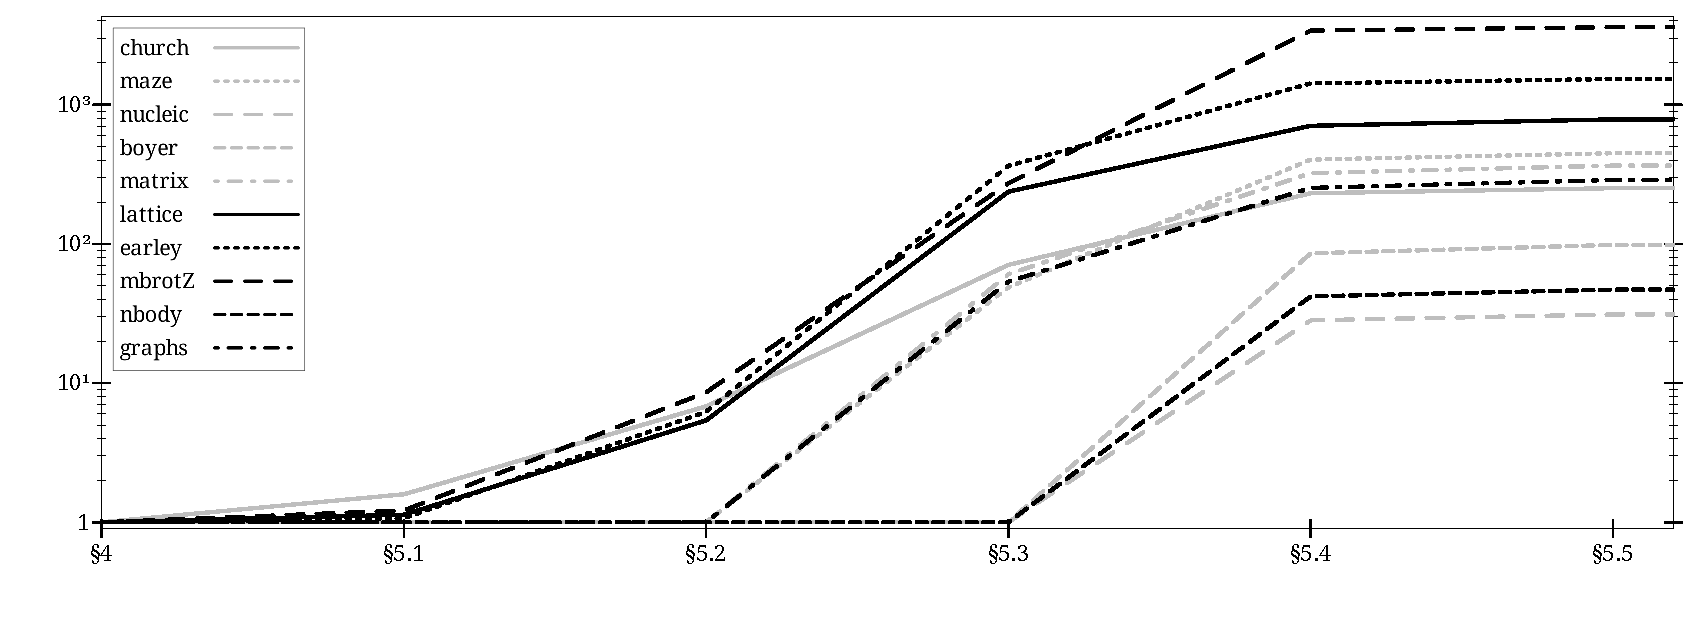
\includegraphics[width=6.5in]{all-relative-time}

  (a) Total analysis time

  \vspace{1em}
  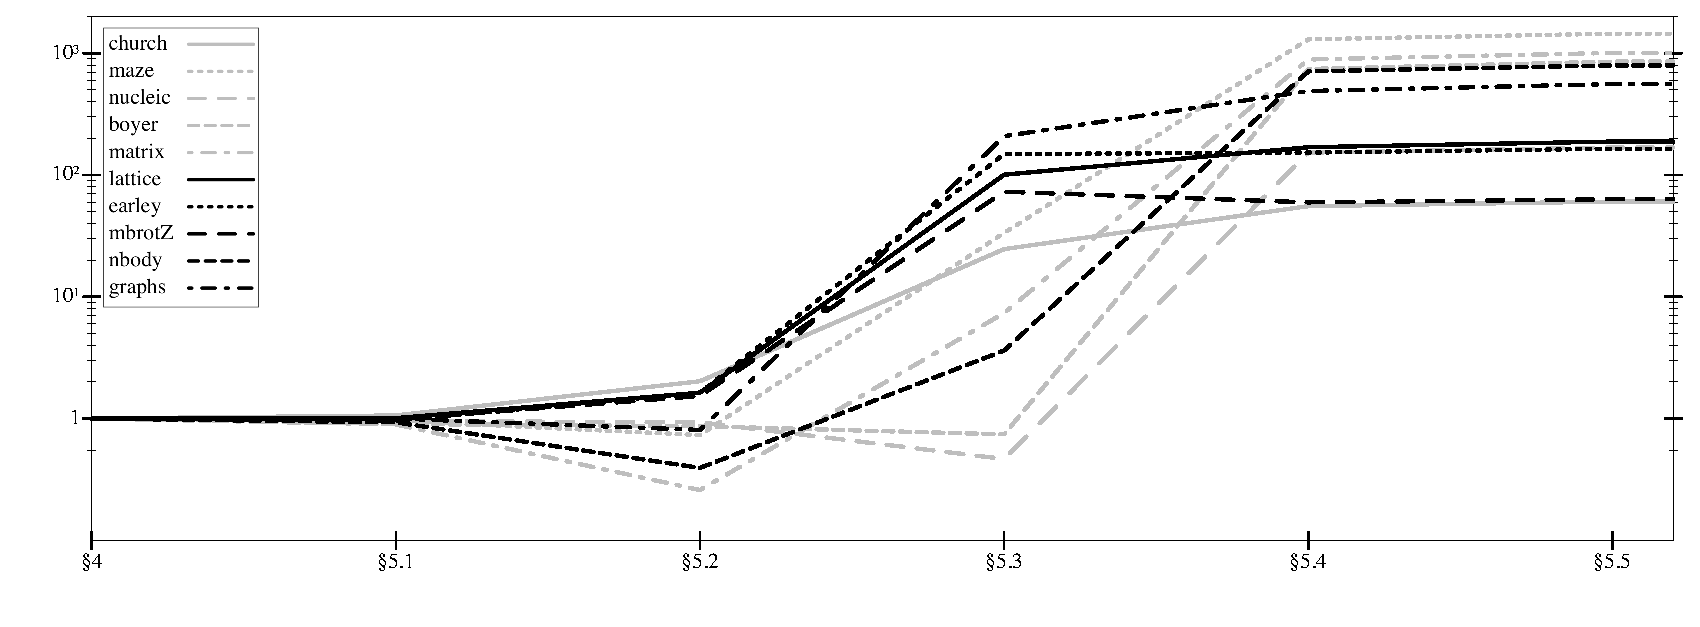
\includegraphics[width=6.5in]{all-relative-speed}

  (b) Rate of state transitions

  \vspace{1em}
  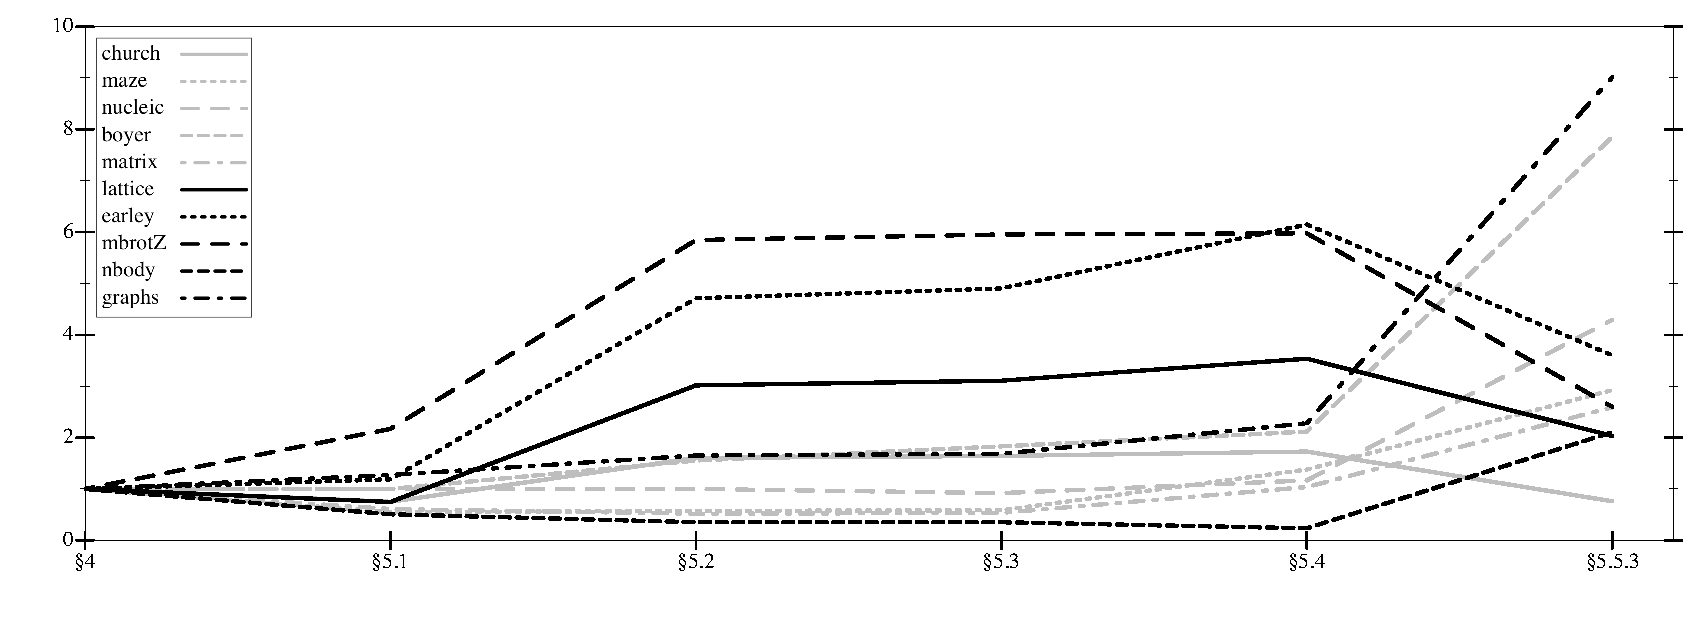
\includegraphics[width=6.5in]{all-relative-space}

  (c) Peak memory usage
\end{center}
\caption{Factors of improvement over baseline for each step of
  optimization (bigger is better).}
\label{fig:bench-all}
\end{figure*}

We evaluated the precision of these techniques with a singleton
variable analysis to find opportunities to inline constants and closed
functions. We found no change in the results across all
implementations, including Shivers' timestamp approximation.

Source code of the implementation and benchmark suite is at:

\begin{center}
\url{https://github.com/dvanhorn/oaam}
\end{center}

\paragraph{Comparison with other flow analysis implementations}

The analysis considered here computes results similar to Earl, et al.'s
0-CFA implementation~\cite{dvanhorn:Earl2012Introspective}, which
times out on the \Church{} benchmark because it does not widen the
store as described for our baseline evaluator.  So even though it
offers a fair point of comparison, a more thorough evaluation is
probably uninformative as the other benchmarks are likely to timeout
as well (and it would require significant effort to extend their
implementation with the features needed to analyze our benchmark
suite).  That implementation is evaluated against much smaller
benchmarks: the largest program is 30 lines.

Vardoulakis and Shivers evaluate their CFA2
analyzer~\cite{dvanhorn:Vardoulakis2011CFA2} against a variant of
0-CFA defined in their framework and the example we draw on is the
largest benchmark Vardoulakis and Shivers consider.  More work would
be required to scale the analyzer to the set of features required by
our benchmarks.

The only analyzers we were able to find that proved capable of
analyzing the full suite of benchmarks considered here were the Soft
Typing system of Wright and
Cartwright~\cite{dvanhorn:Wright1997Practical} and, in many ways its
successor, the Polymorphic splitting system of Wright and
Jagannathan~\cite{dvanhorn:wright-jagannathan-toplas98}.\footnote{This
  is not a coincidence; these papers set a high standard for
  evaluation, which we consciously aimed to approach.}  Unfortunately,
these analyses compute an inherently different and incomparable form
of analysis.  Consequently, we have omitted a complete comparison with
these implementations.  The AAM approach provides more precision in
terms of temporal-ordering of program states, which comes at a cost
that can be avoided in constraint-based approaches.  Consequently
implementation techniques cannot be ``ported'' between these two
approaches.  However, our optimized implementation is within an order
of magnitude of the performance of Wright and Jaganathan's analyzer.
Although we would like to improve this to be more competitive, the
optimized AAM approach still has many strengths to recommend it in
terms of precision, ease of implementation and verification, and rapid
design. We can get closer to their performance by relying on the
representation of addresses and the behavior of $\alloc$ to
pre-allocate most data structures and split the abstract store out
into parts that are more quickly accessed and updated. The first two
of our optimizations can still be applied to an analysis that does
abstract garbage collection~\cite{dvanhorn:Might:2006:GammaCFA},
whereas the polymorphic splitting implementation is tied strongly to a
single-threaded store.

\section{Related work}
\label{sec:related}

\paragraph{Abstracting Abstract Machines}

This work clearly closely follows Van Horn and Might's original papers
on abstracting abstract
machines~\cite{dvanhorn:VanHorn2011Abstracting,dvanhorn:VanHorn2012Systematic},
which in turn is one piece of the large body of research on flow
analysis for higher-order languages (see
Midtgaard~\cite{dvanhorn:Midtgaard2011Controlflow} for a thorough
survey).  The AAM approach sits at the confluence of two major lines
of research: (1) the study of abstract
machines~\cite{dvanhorn:landin-64} and their systematic
construction~\cite{dvanhorn:reynolds-hosc98}, and (2) the theory of
abstract interpretation
\cite{dvanhorn:Cousot:1977:AI,dvanhorn:Cousot1979Systematic}.


\paragraph{Frameworks for flow analysis of higher-order programs}

Besides the original AAM work, the analysis most similar to that
presented in section~\ref{sec:aam} is the infinitary control-flow
analysis of Nielson and Nielson~\cite{dvanhorn:nielson-nielson-popl97}
and the unified treatment of flow analysis by Jagannathan and
Weeks~\cite{dvanhorn:jagannathan-weeks-popl95}.  Both are
parameterized in such a way that in the limit, the analysis is
equivalent to an interpreter for the language, just as is the case
here.  What is different is that both give a constraint-based
formulation of the abstract semantics rather than a finite machine
model.

\paragraph{Abstract compilation}

Boucher and Feeley \cite{dvanhorn:Boucher1996Abstract} introduced the
idea of abstract compilation, which used closure generation
\cite{dvanhorn:Feeley1987Using} to improve the performance of control
flow analysis.  We have adapted the closure generation technique from
compositional evaluators to abstract machines and applied it to similar
effect.

\paragraph{Constraint-based program analysis for higher-order languages}

Constraint-based program analyses
(e.g.~\cite{dvanhorn:nielson-nielson-popl97,dvanhorn:wright-jagannathan-toplas98,dvanhorn:Meunier2006Modular,dvanhorn:steckler-wand-toplas97})
typically compute sets of abstract values for each program point.
These values approximate values arising at run-time for each
program point.  Value sets are computed as the least solution to a set
of (inclusion or equality) constraints.  The
constraints must be designed and proved as a sound approximation of
the semantics.  Efficient implementations of these kinds of analyses
often take the form of worklist-based graph algorithms for constraint
solving, and are thus quite different from the interpreter
implementation.  The approach thus requires effort in constraint
system design and implementation, and the resulting system require
verification effort to prove the constraint system is sound and that
the implementation is correct.

This effort increases substantially as the complexity of the analyzed
language increases.  Both the work of maintaining the concrete
semantics and constraint system (and the relations between them) must
be scaled simultaneously.  However, constraint systems, which have
been extensively studied in their own right, enjoy efficient
implementation techniques and can be expressed in declarative logic
languages that are heavily
optimized~\cite{dvanhorn:bravenboer-smaragdakis-oopsla09}.
Consequently, constraint-based analyses can be computed quickly.  For
example, Jagannathan and Wright's polymorphic splitting
implementation~\cite{dvanhorn:wright-jagannathan-toplas98} analyses
the \Church{} benchmark about 25 times faster than the fastest
implementation considered here.  These analyses compute very different
things, so the performance comparison is not apples-to-apples.

The AAM approach, and the state transition graphs it generates, encodes
temporal properties not found in classical constraint-based analyses
for higher-order programs.
%
Such analyses (ultimately) compute judgments on program terms and
contexts, e.g., at expression $e$, variable $x$ may have value $v$.
%
The judgments do not relate the order in which expressions and context
may be evaluated in a program, e.g., it has nothing
to say with regard to question like, ``Do we always evaluate $e_1$
before $e_2$?'' or ``Is it always the case that a file handle is
opened, read and then closed in that order?''
%
The state transition graphs can answer these kinds of queries, but
this does not come for free: respecting temporal order imposes an
order in which states and terms may be evaluated \emph{during} the
analysis.

\section{Conclusion}
\label{sec:conclusion}

Abstract machines are not only a good model for rapid analysis
development, they can be systematically developed into efficient
algorithms that can be proved correct. We view the primary
contribution of this work as a systematic path that eases the design,
verification, and implementation of analyses using the abstracting
abstract machine approach to within a factor of performant
constraint-based analyses.

%% \acks Sam Tobin-Hochstadt for encouragement and feedback -- he was
%% the first to prompt us to look into how make effective
%% implementations of the AAM approach.

%% Vincent St Amour and Mitchell Wand for feedback on early drafts.
%% Greg Morrisset and Matthias Felleisen for discussions.

%% NSF, DARPA


\paragraph{Acknowledgments}

We thank Suresh Jagannathan for providing source code to the
polymorphic splitting
analyzer~\cite{dvanhorn:wright-jagannathan-toplas98} and Ilya Sergey
for the introspective pushdown
analyzer~\cite{dvanhorn:Earl2012Introspective}.


\balance
\bibliographystyle{plain}
%\documentclass[preprint,onecolumn,9pt]{sigplanconf} %{onecol}
\usepackage{alltt,mathpartir}
\usepackage{amsmath,amsthm}
\usepackage{amssymb}
\usepackage{stmaryrd}
\usepackage{url}
\usepackage{graphicx}
\usepackage{balance}
\usepackage{calc}

\newtheorem{theorem}{Theorem}
\newtheorem{lemma}{Lemma}

\newcommand{\naive}{naive}
\newcommand{\naively}{naively}
\newcommand{\Naive}{Naive}
\newcommand{\Naively}{Naively}
% \usepackage{xltxtra}
% \setmonofont[Scale=MatchLowercase]{DejaVu Sans Mono}
%
\newcommand{\superscript}[1]{\ensuremath{^{#1}}}
\newcommand{\subscript}[1]{\ensuremath{_{#1}}}
\newcommand{\tuple}[3][\ ]{{\tt #2{#1}}({#3})}

% Values
\newcommand{\clos}[1]{\tuple{clos}{#1}}
\newcommand{\rlos}[1]{\tuple{rlos}{#1}}

% States
\newcommand{\ev}[2][\ ]{\tuple[#1]{ev}{#2}}
\newcommand{\co}[1]{\tuple{co}{#1}}
\newcommand{\ap}[2][\ ]{\tuple[#1]{ap}{#2}}
\newcommand{\ans}[1]{\tuple{ans}{#1}}

% Continuations
\newcommand{\kmt}{\tt mt}
\newcommand{\kar}[2][\ ]{\tuple[#1]{ar}{#2}}
\newcommand{\kfn}[2][\ ]{\tuple[#1]{fn}{#2}}
\newcommand{\kif}[2][\ ]{\tuple[#1]{fi}{#2}}
\newcommand{\kuop}[2][\ ]{\tuple[#1]{oa}{#2}}
\newcommand{\kbopa}[2][\ ]{\tuple[#1]{oa1}{#2}}
\newcommand{\kbopb}[2][\ ]{\tuple[#1]{oa2}{#2}}

% Implementation forms
\newcommand{\generator}{{\tt generator}}
\newcommand{\yield}[1]{{\tt yield} #1}

% Syntax
\newcommand{\syntax}[1]{{\tt #1}}
\newcommand{\sapp}[3][\ ]{\tuple[#1]{app}{#2,#3}}
\newcommand{\slam}[3][\ ]{\tuple[#1]{lam}{#2,#3}}
\newcommand{\srec}[4][\ ]{\tuple[#1]{rec}{#2,#3,#4}}
\newcommand{\svar}[2][\ ]{\tuple[#1]{var}{#2}}
\newcommand{\snum}[2][\ ]{\tuple[#1]{num}{#2}}
\newcommand{\sbln}[2][\ ]{\tuple[#1]{bool}{#2}}
\newcommand{\sif}[4][\ ]{\tuple[#1]{if}{#2,#3,#4}}
\newcommand{\sop}[2][\ ]{\tuple[#1]{op}{#2}}
\newcommand{\sopu}[3][\ ]{\tuple[#1]{op}{#2,#3}}
\newcommand{\sopb}[4][\ ]{\tuple[#1]{op2}{#2,#3,#4}}
\newcommand{\strue}{{\tt tt}}
\newcommand{\sfalse}{{\tt ff}}
\newcommand{\saddone}{{\tt add1}}
\newcommand{\ssubone}{{\tt sub1}}
\newcommand{\szerohuh}{\syntax{zero?}}
\newcommand{\szero}{\syntax{0}}
\newcommand{\slit}[2][\ ]{\tuple[#1]{lit}{#2}}

\newcommand{\sNum}{\syntax{Z}}

% Metavariables
\newcommand{\maddr}{a}
\newcommand{\mvar}{x}
\newcommand{\mvarf}{f}
\newcommand{\mexp}{e}
\newcommand{\mexpi}[1]{e_{#1}}
\newcommand{\mexpf}{f}
\newcommand{\menv}{\rho}
\newcommand{\mkont}{\kappa}
\newcommand{\msto}{\sigma}
\newcommand{\mop}{o}
\newcommand{\mval}{v}
\newcommand{\mnum}{z}
\newcommand{\mbln}{b}
\newcommand{\mvalx}[1]{#1}
\newcommand\machstep{\longmapsto}
\newcommand\multimachstep{\longmapsto\!\!\!\!\!\rightarrow}
\newcommand{\mlit}{l}
\newcommand{\mstate}{\varsigma}
\newcommand{\mcomp}{k}
\newcommand{\mcompi}[1]{\mcomp_{#1}}
\newcommand{\interpdelta}{\Delta}

\newcommand{\compile}[1]{\llbracket#1\rrbracket}

\newcommand{\mlab}{{\ell}}
\newcommand{\mcntr}{{\delta}}
\newcommand{\mtcntr}{{\epsilon}}


\begin{document}

\conferenceinfo{WXYZ '05}{date, City.}
\copyrightyear{2005}
\copyrightdata{[to be supplied]}

% \titlebanner{banner above paper title}        % These are ignored unless
% \preprintfooter{short description of paper}   % 'preprint' option specified.

%\title{Provably Correct, Low-Cost Optimizations for Abstract Abstract Machines}
\title{Correctly Optimizing Abstract Abstract Machines}

\authorinfo{J. Ian Johnson \and Nicholas Labich \and Matthew Might \and David Van Horn}
           {}
           {}
%% \authorinfo{J. Ian Johnson}
%%            {Northeastern University}
%%            {ianj@ccs.neu.edu}
%% \authorinfo{Nicholas Labich}
%%            {Northeastern University}
%%            {labichn@ccs.neu.edu}
%% \authorinfo{Matthew Might}
%%            {University of Utah}
%%            {might@cs.utah.edu}
%% \authorinfo{David Van Horn}
%%            {Northeastern University}
%%            {dvanhorn@ccs.neu.edu}
\maketitle

\begin{abstract}
The technique of \emph{abstracting abstract machines} (AAM) provides a
systematic approach for deriving computable approximations of
evaluators that are easily proved sound.
%
This article contributes a complementary step-by-step process for
subsequently going from a \naive{} analyzer derived under the AAM
approach, to an efficient and correct implementation.  The end result
of the process is a two to three order-of-magnitude improvement over
the systematically derived analyzer, making it competitive with
hand-optimized implementations that compute fundamentally less precise
results.
\end{abstract}

%% \category{CR-number}{subcategory}{third-level}

%% \terms
%% term1, term2

%% \keywords
%% keyword1, keyword2

\section{Introduction}

Program analysis provides sound predictive models of program behavior, but
in order for such models to be effective, they must be efficiently
computable and correct.  Past approaches to designing program analysis
have often featured abstractions that are far removed from the
original language semantics, requiring ingenuity in their construction
and effort in their verification.
%
The \emph{abstracting abstract machines} (AAM)
approach~\cite{dvanhorn:VanHorn2011Abstracting,dvanhorn:VanHorn2012Systematic}
to deriving program analyses provides an alternative: a systematic way
of transforming a programming language semantics in the form of an
abstract machine into a family of abstract interpreters.  It thus reduces
the burden of constructing and verifying the soundness of an abstract
interpreter.
%

%
% Specifically, these policies tune precision for control,
% the environment, the store, and base value domains.

By taking a
machine-oriented view of computation, AAM makes it possible to design,
verify, and implement program analyzers for realistic language
features typically considered difficult to model.  The approach was
originally applied to features such as higher-order functions,
stack inspection, exceptions, laziness, first-class continuations, and
garbage collection.  It has since been used to verify actor-
\cite{local:DOsualdo:12A} and
thread-based~\cite{dvanhorn:Might2011Family} parallelism and
behavioral contracts~\cite{dvanhorn:TobinHochstadt2012Higherorder}; it
has been used to model Coq~\cite{local:harvard},
Dalvik~\cite{local:dalvik}, Erlang~\cite{local:DOsualdo:12B},
JavaScript~\cite{local:DBLP:journals/corr/abs-1109-4467}, and
Racket~\cite{dvanhorn:TobinHochstadt2012Higherorder}.

The primary strength of the approach is that abstract interpreters can
be easily derived through a small number of steps from existing
machine models.  Since the relationships between abstract machines and
higher-level semantic models---such as definitional
interpreters~\cite{dvanhorn:reynolds-hosc98}, structured operational
semantics~\cite{dvanhorn:Plotkin1981Structural}, and reduction
semantics~\cite{dvanhorn:Felleisen2009Semantics}---are well
understood~\cite{dvanhorn:Danvy:DSc}, it is possible to navigate from
these high-level semantic models to sound program analyzers in a
systematic way.  Moreover, since these analyses so closely resemble a
language's interpreter (a) implementing an analysis requires little
more than implementing an interpreter, (b) a single implementation can
serve as both an interpreter and analyzer, and (c) verifying the
correctness of the implementation is straightforward.

Unfortunately, the AAM approach yields analyzers with poor performance
relative to hand-optimized analyzers.
%
Our work takes aim squarely at this ``efficiency gap,'' and narrows it
in an equally systematic way through a number of simple steps, many of
which are inspired by run-time implementation techniques such as
laziness and compilation to avoid interpretative overhead.  Each of
these steps is proven correct, so the end result is an implementation
that is trustworthy and efficient.

In this article, we develop a systematic approach to deriving a
practical implementation of an abstract-machine-based analyzer using
mostly semantic means rather than tricky engineering. Our goal is to
empower programming language implementers and researchers to explore
and convincingly exhibit their ideas with a low barrier to entry. The
optimizations we describe are widely applicable and apparently
effective to scale far beyond the size of programs typically considered
in the recent literature on flow analysis for functional languages.

\section{At a glance}

\begin{figure}[t]
\begin{center}
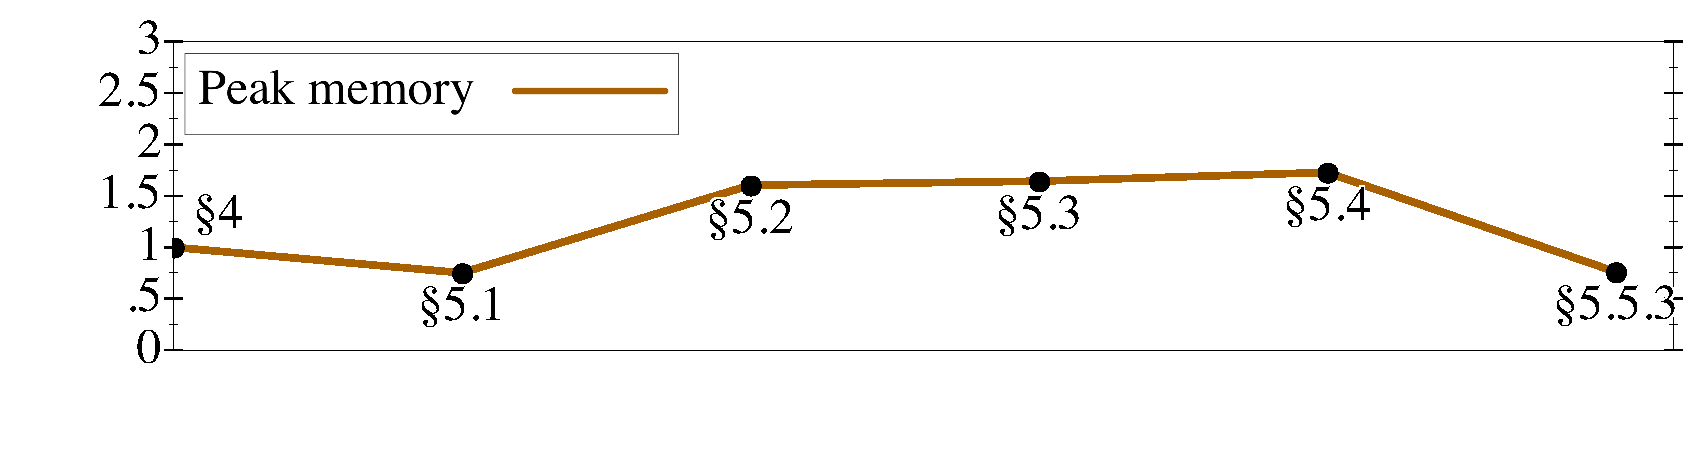
\includegraphics[width=3.2in]{church-relative-space}
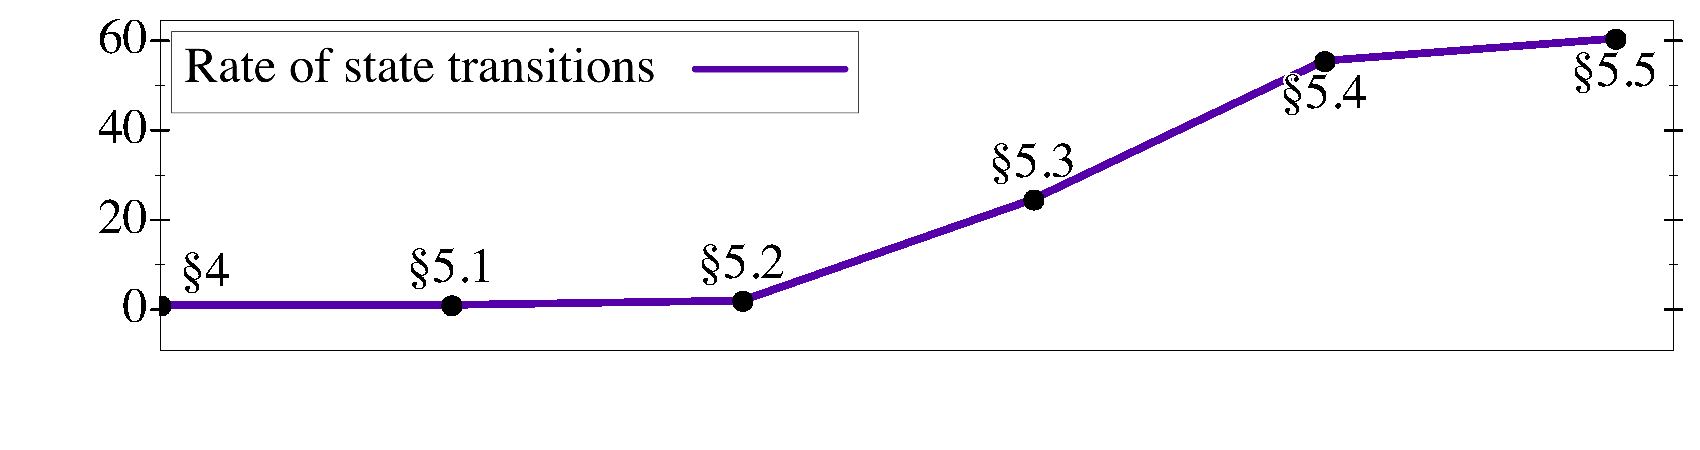
\includegraphics[width=3.2in]{church-relative-speed}
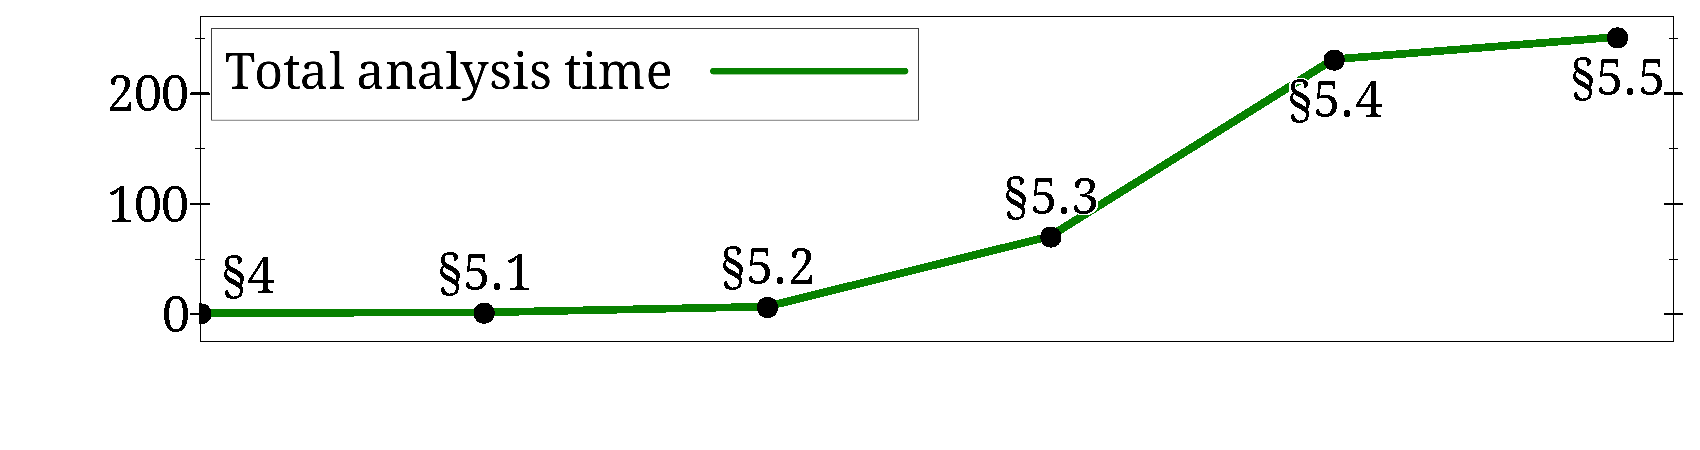
\includegraphics[width=3.2in]{church-relative-time}
\vspace{-1.5em}
\end{center}
\caption{Factor improvements over the baseline analyzer for the
  \Church{} benchmark in terms of peak memory usage, the rate of state
  transitions, and total analysis time. (Bigger is better.) Each point
  is marked with the section that introduces the optimization.}
\label{fig:churchtime}
\end{figure}


We start with a quick review of the AAM approach to develop an
analysis framework and then apply our step-by-step optimization
techniques in the simplified setting of a core functional language.
This allows us to explicate the optimizations with a minimal amount of
inessential technical overhead.  Following that, we scale this
approach up to an analyzer for a realistic untyped, higher-order
imperative language with a number of interesting features and then
measure improvements across a suite of benchmarks.

At each step during the initial presentation and development, we
evaluated the implementation on a set of benchmarks. The highlighted
benchmark in figure \ref{fig:churchtime} is from Vardoulakis and
Shivers~\cite{dvanhorn:Vardoulakis2011CFA2} that tests distributivity
of multiplication over addition on Church numerals.  For the
step-by-step development, this benchmark is particularly informative:
\begin{enumerate}
\item it can be written in most modern programming languages,
%
\item it was designed to stress an analyzer's ability to deal with
  complicated environment and control structure arising from the use
  of higher-order functions to encode arithmetic, and
%
\item its improvement is about median in the benchmark suite
  considered in section~\ref{sec:eval}, and thus it serves as a good
  sanity check for each of the optimization techniques considered.
\end{enumerate}

We start, in section~\ref{sec:aam}, by developing an abstract
interpreter according to the AAM approach.  In the initial
abstraction, each state carries a store (what is called per-state
store variance). The space of stores is exponential in size; without
further abstraction, the analysis is exponential and thus cannot
analyze the example in a reasonable amount of time.  In
section~\ref{sec:baseline}, we perform a further abstraction by
widening the store.  The resulting analyzer sacrifices precision for
speed and is able to analyze the example in about 1 minute.  This step
is described by Van Horn and Might~\cite[\S
3.5--6]{dvanhorn:VanHorn2012Systematic} and is necessary to make even
small examples feasible.  We therefore take a widened interpreter as
the baseline for our evaluation.

Section~\ref{sec:opt} gives a series of simple abstractions and
implementation techniques that, in total, speed up the analysis by
nearly a factor of 500, dropping the analysis time to a fraction of a
second.  Figure~\ref{fig:churchtime} shows the step-wise improvement
of the analysis time for this example.

\begin{figure}[t]
\begin{center}
\begin{tabular}{ccc}
\raisebox{1ex-\height}{
\includegraphics[height=3.5in]{introspective-base.pdf}}
&
\raisebox{1ex-\height}{
\includegraphics[height=3.5in]{introspective-lazy.pdf}}
&
\raisebox{1ex-\height}{
\includegraphics[height=3in]{introspective-lazyc.pdf}}
\\
(a) Baseline
&
(b) Lazy
&
(c) Compiled (\& lazy)
\end{tabular}
\end{center}
\caption{Example state graphs for the program above.  Part (a) shows
  the result of the baseline analyzer.  It has long ``corridor''
  transitions and ``diamond'' subgraphs that fan-out from
  nondeterminism and fan-in from joins.  Part (b) shows the result of
  performing nondeterminism lazily and thus avoids many of the diamond
  subgraphs.  Part (c) shows the result of abstract compilation that
  removes interpretive overhead in the form of intermediate states,
  thus minimizing the corridor transitions.  The end result is a more
  compact abstraction of the program that can be generated faster.}
\label{fig:state-graphs}
\end{figure}

The AAM approach, in essence, does the following: it takes a
machine-based view of computation and turns it into a \emph{finitary
  approximation} by bounding the size of the store.  With a limited
address space, the store must map addresses to \emph{sets} of values.
Store updates are interpreted as joins, and store dereferences are
interpreted by non-deterministic choice of an element from a set.  The
result of analyzing a program is a finite directed graph where nodes
in the graph are (abstract) machine states and edges denote machine
transitions between states.

The techniques we propose for optimizing analysis fall into the
following categories:
\begin{enumerate}
\item generate fewer states by avoiding the eager exploration of
  non-deterministic choices that will later collapse into a single
  join point.  We accomplish this by applying lazy evaluation
  techniques so that non-determinism is evaluated \emph{by need}.

\item generate fewer states by avoiding unnecessary, intermediate
  states of a computation.  We accomplish this by applying compilation
  techniques from functional languages to avoid interpretive overhead
  in the machine transition system.

\item generate states faster.  We accomplish this by better algorithm
  design in the fixed-point computation we use to generate state graphs.
\end{enumerate}
Figure~\ref{fig:state-graphs} shows the effect of (1) and (2) for a
small example due to Earl, et
al.~\cite{dvanhorn:Earl2012Introspective}.
By generating significantly fewer states at a significantly faster
rate, we are able to achieve large performance improvements in terms
of both time and space.

Section~\ref{sec:eval} describes the evaluation of each optimization
technique applied to an implementation supporting a more realistic set
of features, including mutation, first-class control, compound data, a
full numeric tower and many more forms of primitive data and
operations.
%
We evaluate this implementation against a set of benchmark programs
drawn from the literature.
%
For all benchmarks, the optimized analyzer outperforms the baseline
by at least a factor of
% 475
two to
% 4,382
three orders of magnitude.

Section~\ref{sec:related} relates this work to the literature and
section~\ref{sec:conclusion} concludes.

%\newpage
\section{Abstract interpretation of ISWIM}
\label{sec:aam}

In this section, we give a brief review of the AAM approach by
defining a sound analytic framework for a core higher-order functional
language: Landin's ISWIM~\cite{dvanhorn:Landin1966Next}.  In the
subsequent sections, we will explore optimizations for the analyzer in
this simplified setting, but scaling these techniques to realistic
languages is straightforward and has been done for the analyzer
evaluated in section~\ref{sec:eval}.

ISWIM is a family of programming languages parameterized by a set of
base values and operations.  To make things concrete, we consider a
member of the ISWIM family with integers, booleans, and a few
operations.
%
Figure~\ref{fig:syntax} defines the syntax of ISWIM.  It
includes variables, literals (either integers, booleans, or
operations), $\lambda$-expressions for defining procedures, procedure
applications, and conditionals.  Expressions carry a label, $\mlab$,
which is drawn from an unspecified set and denotes the source location
of the expression; labels are used to disambiguate distinct, but
syntactically identical pieces of syntax.  We omit the label
annotation in contexts where it is irrelevant.

\begin{figure}
\[
\begin{array}{l@{\qquad}rcl}
\text{Expressions} & \mexp &=& \svar[^\mlab]\mvar\\
&&|& \slit[^\mlab]\mlit\\
&&|& \slam[^\mlab]\mvar\mexp\\
&&|& \sapp[^\mlab]\mexp\mexp \\
&&|& \sif[^\mlab]\mexp\mexp\mexp \\
\text{Variables}&\mvar &=& \syntax{x}\ |\ \syntax{y}\ |\ \dots\\
\text{Literals}&\mlit &=& \mnum\ |\ \mbln\ |\ \mop\\
\text{Integers}&\mnum &=& \syntax{0}\ |\ \syntax{1}\ |\ \syntax{-1}\ |\ \dots\\
\text{Booleans}&\mbln &=& \strue\ |\ \sfalse\\
\text{Operations}&\mop &=& \syntax{zero?}\ |\ \syntax{add1}\ |\ \syntax{sub1}\ |\ \dots
\end{array}
\]
\caption{Syntax of ISWIM}
\label{fig:syntax}
\end{figure}

\begin{figure}
\[
\begin{array}{l@{\qquad}rcl}
\text{Values} & \mval,\mvalx{u} &=& \clos{\mvar,\mexp,\menv}\ |\ \mlit\ |\ \mkont\\
\text{States} & \mstate &=& \ev{\mexp,\menv,\msto,\mkont}\\
                       &&|& \co{\mkont,\mval,\msto}\\
                       &&|& \ap{\mval,\mval,\msto,\mkont}\\
\text{Continuations} & \mkont &=& \kmt\\
&&|& \kfn{\mval,\mkaddr}\\
&&|& \kar{\mexp,\menv,\mkaddr}\\
&&|& \kif{\mexp,\mexp,\menv,\mkaddr}\\
\text{Addresses} &\maddr&\in&\Addr \\
\text{Environments} &\menv&\in& \Var \rightharpoonup \Addr\\
\text{Stores} &\msto&\in& \Addr \rightharpoonup \mathcal{P}(\Value)
\end{array}
\]
\caption{Abstract machine components}
\label{fig:domains}
\end{figure}


The semantics are defined in terms of a machine model.  The machine
components are defined in figure~\ref{fig:domains};
figure~\ref{fig:aam} defines the transition relation.  The evaluation
of a program is defined as its set of traces that arise from iterating the
machine transition relation.  The
machine is a very slight variation on a standard abstract machine for
ISWIM in ``eval, continue, apply'' form~\cite{dvanhorn:Danvy:DSc}.  It
can be systematically derived from a definitional interpreter through
a continuation-passing style transformation and defunctionalization,
or from a structural operational semantics using the refocusing
construction of Danvy and
Nielsen~\cite{dvanhorn:Danvy-Nielsen:RS-04-26}.

Compared with the standard machine semantics, this definition is
different in the following ways, which make it abstractable as a
program analyzer:
\begin{itemize}
\item the store maps addresses to \emph{sets} of values,\footnote{
More generally, we can have stores map to any domain that forms
 a Galois connection with values, enabling $\interpdelta$ to
produce elaborate abstractions of base values (e.g., interval or octagon
abstractions). We use sets of values for a simpler exposition.
} not
  single values,

\item continuations are heap-allocated, not stack-allocated,
\item there are ``timestamps'' ($\mcntr \in \Counter$) and syntax
  labels ($\mlab$) threaded through the computation, and
\item the machine is implicitly parameterized by the functions
  $\alloc$, $\allockont$, $\tick$, $\interpdelta$, and spaces
  $\Addr$, $\Counter$ (and initial $\mcntr_0 \in \Counter$).
\end{itemize}


\begin{figure}
\begin{gather*}
\begin{align*}
\traces(\mexp) &= \{ \ev[^{\mtcntr}]{\mexp,\varnothing,\varnothing,\kmt} \multimachstep \mstate \} \text{ where }
\end{align*}
\\[2mm]
\begin{array}{@{}r@{\ }c@{\ }l@{}}
\mstate &\machstep&\mstate' \text{ defined to be the following} \\
&&\text{let } \mcntr' =\tick(\mstate) \\
%% EVAL
\ev{\svar\mvar,\menv,\msto,\mkont} &\machstep&
\co{\mkont,\mval,\msto}
\text{ if }\mval \in \msto(\menv(\mvar))
\\
\ev{\slit\mlit,\menv,\msto,\mkont} &\machstep&
\co{\mkont,\mlit,\msto}
\\
\ev[^\mcntr]{\slam\mvar\mexp,\menv,\msto,\mkont} &\machstep&
\co[^{\mcntr'}]{\mkont,\clos{\mvar,\mexp,\menv},\msto}
\\
\ev[^\mcntr]{\sapp[^\mlab]{\mexpi0}{\mexpi1},\menv,\msto,\mkont} &\machstep&
\ev[^{\mcntr'}]{\mexpi{0},\menv,\msto',\kar[_\mlab^\mcntr]{\mexpi{1},\menv,\mkaddr}}
\\
&&
\text{ where }\mkaddr = \allockont^\mcntr_\mlab(\msto,\mkont) \\
&&\phantom{\text{ where }}\msto' = \msto\sqcup[\mkaddr \mapsto \setof{\mkont}]
\\
\ev[^\mcntr]{\sif[^\mlab]{\mexpi0}{\mexpi1}{\mexpi2},\menv,\msto,\mkont} &\machstep&
\ev[^{\mcntr'}]{\mexpi0,\menv,\msto',\kif[^\mcntr]{\mexpi1,\mexpi2,\menv,\mkaddr}}
\\
&&
\text{ where }\mkaddr = \allockont^\mcntr_\mlab(\msto,\mkont) \\
&&\phantom{\text{ where }}\msto' = \msto\sqcup[\mkaddr \mapsto \setof{\mkont}]
\\[2mm]
%% CONTINUE
\co{\kmt,\mval,\msto} &\machstep&
\ans{\msto,\mval}
\\
\co{\kar[^\mcntr_\mlab]{\mexp,\menv,\mkaddr},\mval,\msto} & \machstep&
\ev[^\mcntr]{\mexp,\menv,\msto,\kfn[^\mcntr_\mlab]{\mval,\mkaddr}}
\\
\co{\kfn[^\mcntr_\mlab]{{\mvalx{u}},\mkaddr},\mval,\msto} & \machstep&
\ap[^\mcntr_\mlab]{\mvalx{u},\mval,\mkont,\msto}
\text{ if }\mkont \in \msto(\mkaddr)
\\
\co{\kif[^\mcntr]{\mexpi0,\mexpi1,\menv,\mkaddr},\strue,\msto} & \machstep&
\ev[^{\mcntr'}]{\mexpi0,\menv,\msto,\mkont}
\text{ if }\mkont\in\msto(\mkaddr)
\\
\co{\kif[^\mcntr]{\mexpi0,\mexpi1,\menv,\mkaddr},\sfalse,\msto} & \machstep&
\ev[^{\mcntr'}]{\mexpi1,\menv,\msto,\mkont}
\text{ if }\mkont\in\msto(\mkaddr)
\\[2mm]
%% APPLY
\ap[^\mcntr_\mlab]{\clos{\mvar,\mexp,\menv},\mval,\msto,\mkont} & \machstep&
\ev[^{\mcntr'}\!]{\mexp,\menv',\msto',\mkont}
\\
&&\text{ where } \maddr  =\alloc(\mstate) \\
&&\phantom{\text{ where }} \menv' = \menv[\mvar\mapsto\maddr] \\
&&\phantom{\text{ where }} \msto' = \msto\sqcup[\maddr\mapsto\{\mval\}] \\
\\
\ap[^\mcntr_\mlab]{\mop,\mval,\msto,\mkont} & \machstep&
\co{\mkont,\mval',\msto}
\text{ if } \mval'\in\interpdelta(\mop,\mval)
\end{array}
\end{gather*}
\caption{Abstract abstract machine for ISWIM}
\label{fig:aam}
\end{figure}


\paragraph{Concrete interpretation} To characterize concrete interpretation, set the implicit
parameters of the relation given in figure~\ref{fig:aam} as follows:
\begin{align*}
\alloc(\mstate) &= \maddr \mbox{ where } \maddr \notin \text{ the } \msto \text{ within } \mstate \\
\allockont^\mcntr_\mlab(\msto,\mkont) &=\mkaddr \mbox{ where } \mkaddr \notin \msto
\end{align*}
These functions appear to ignore $\mlab$ and $\mcntr$, but they can be
used to determinize the choice of fresh addresses. The $\sqcup$ on
stores in the figure is a point-wise lifting of $\cup$: $\msto \sqcup \msto' =
\lambda \maddr. \msto(\maddr) \cup \msto'(\maddr)$. The resulting
relation is non-deterministic in its choice of addresses, however it
must always choose a fresh address when allocating a continuation or
variable binding.  If we consider machine states equivalent up to
consistent renaming and fix an allocation scheme, this relation
defines a deterministic machine (the relation is really a function).

The interpretation of primitive operations is defined by setting
$\interpdelta$ as follows:
\begin{align*}
\mnum+1 &\in \interpdelta(\saddone,\mnum) &
\mnum-1 &\in \interpdelta(\ssubone,\mnum)\\
\strue &\in \interpdelta(\szerohuh,\szero) &
\sfalse &\in \interpdelta(\szerohuh,\mnum)\text{ if }\mnum\neq \szero\\
\end{align*}


\paragraph{Abstract interpretation} To characterize abstract
interpretation, set the implicit parameters just as above, but drop
the $\maddr \not\in \msto$ condition. The $\interpdelta$ relation takes some care
to not make the analysis run forever; a simple instantiation is a flat
abstraction where arithmetic operations return an abstract top element
$\sNum$, and $\szerohuh$ returns both $\strue$ and $\sfalse$ on
$\sNum$.  This family of interpreters is also non-deterministic in
choices of addresses, but it is free to choose addresses that are
already in use.  Consequently, the machines may be non-deterministic
when multiple values reside in a store location.

It is important to recognize from this definition that \emph{any}
allocation strategy is a sound abstract
interpretation~\cite{dvanhorn:Might2009Posteriori}.  In particular,
concrete interpretation is a kind of abstract interpretation.  So is
an interpretation that allocates a single cell into which all bindings
and continuations are stored.  The former is an abstract
interpretation that is non-computable and gives only the ground truth
of a programs behavior; the latter is an abstract interpretation
that is easy to compute but gives little information.  Useful program
analyses lay somewhere in between and can be characterized by their
choice of address representation and allocation strategy.  Uniform
\(k\)-CFA~\cite{dvanhorn:nielson-nielson-popl97}, presented next, is one such analysis.

\paragraph{Uniform \(k\)-CFA} To characterize uniform \(k\)-CFA, set the allocation
strategy as follows, for a fixed constant \(k\):

\begin{align*}
\Counter &= \Label^* \\
\mtcntr &= \epsilon \\
\alloc(\ev[^\mcntr]{\sapp[^\mlab]{\mexpi0}{\mexpi1},\menv,\msto,\mkont} &= \mlab\mcntr \\
\alloc(\ap[^\mcntr_\mlab]{\clos{\mvar,\mexp,\menv},\mval,\msto,\mkont}) &= \mvar\kpush[_k]{\mlab\mcntr} \\
\allockont^\mcntr_\mlab(\msto,\mkont) &= \mlab\mcntr \\
\tick(\ev[^\mcntr]{\mexp,\menv,\msto,\mkont}) &= \mcntr \\
\tick(\co{\kar[^\mcntr]{\mexp,\menv,\mkaddr},\mval,\msto}) &= \mcntr \\
\tick(\ap[^\mcntr_\mlab]{\mvalx{u},\mval,\mkont}) &= \kpush[_k]{\mlab\mcntr} \\
  \kpush[_0]{\mcntr} &= \kpush[_k]{\mtcntr} = \mtcntr \\
  \kpush[_{k+1}]{\mlab\mcntr} &= \mlab\kpush[_k]{\mcntr} \\
\end{align*}
The \(\lfloor\cdot\rfloor_k\) notation denotes the truncation of a list
of symbols to the leftmost \(k\) symbols.

All that remains is the interpretation of primitives.  For abstract
interpretation, we set $\interpdelta$ to the function that returns
$\sNum$ on all inputs---a symbolic value we interpret as denoting the
set of all integers.

At this point, we have abstracted the original machine to one which
has a finite state space for any given program, and thus forms the
basis of a sound, computable program analyzer for ISWIM.

\section{From machine semantics to baseline analyzer}
\label{sec:baseline}

The uniform $k$-CFA allocation strategy would make $\traces$ in figure
\ref{fig:aam} a computable abstraction of possible executions, but one
that is too inefficient to run, even on small examples.  Through this
section, we explain a succession of approximations to reach a more
appropriate baseline analysis.
%
We ground this path by first formulating the analysis in terms of a
classic fixed-point computation.


\subsection{Static analysis as fixed-point computation}
\label{sec:fixpoint}

Conceptually, the AAM approach calls for computing an analysis as a
graph exploration: (1) start with an initial state, and (2) compute
the transitive closure of the transition relation from that state. All
visited states are potentially reachable in the concrete, and all
paths through the graph are possible traces of execution.

We can cast this exploration process in terms of a fixed-point calculation.
%
Given the initial state $\mstate_0$ and the transition relation $\machstep$,
we define the global transfer function:
\begin{equation*}
 F_{\mstate_0} : \wp(\State) \times \wp(\State\times\State) \to \wp(\State) \times \wp(\State\times\State)\text.
\end{equation*}
Internally, this global transfer function computes the successors of all supplied states, and then includes the initial state:
\begin{align*}
  F_{\mstate_0}(V,E) &= (\{ \mstate_0 \} \cup V', E') \\
    E' &= \setof{ (\mstate,\mstate') \mid \mstate \in V \text{ and } \mstate \machstep \mstate'} \\
    V' &= \setof{ \mstate' \mid (\mstate,\mstate') \in E'}
\end{align*}
Then, the evaluator for the analysis computes the least fixed-point of the global transfer function:
\begin{equation*}
 \eval(\mexp) = \mathrm{lfp}(F_{\mstate_0})\text{,}
\end{equation*}
where $\mstate_0 = \ev[^\mtcntr]{\mexp, \varnothing, \varnothing, \kmt}$.

The possible traces of execution tell us the most about a program, so
we take $\traces(\mexp)$ to be the (regular) set of paths through the
computed graph. We elide the construction of the set of edges in this paper.

To conduct this \naive{} exploration on the \Church{} example would require
considerable time.  Even though the state space is finite, it is exponential in
the size of the program.  Even with $k = 0$, there are exponentially many
stores in the AAM framework.

In the next subsection, we fix this with store widening to reach polynomial
(albeit of high degree) complexity.
%
This widening effectively lifts the store out of individual states to create
a single, global shared store for all.


\subsection{Store widening}
\label{sec:storewiden}

A common technique to accelerate convergence in flow analyses is to share a
common, global store.
%
To retain soundness, this store grows monotonically.
%
Formally, we can cast this optimization as a second abstraction or as the
application of a widening operator during the fixed-point iteration.
%
In the ISWIM language, such a widening makes 0-CFA quartic in the size of the
program.
%
Thus, complexity drops from intractable exponentiality to a merely
daunting polynomial.

Since we can cast this optimization as a widening, there is no need to change
the transition relation itself.
%
Rather, what changes is the structure of the fixed-point iteration.
%
In each pass, the algorithm will collect all newly produced stores and join
them together.
%
Then, before each transition, it will install this joined store into current
state.

To describe this process, AAM defined a transformation of the reduction relation so that it operates on
a pair of a set of contexts ($C$) and a store ($\sigma$).
%
A context includes all non-store components, \emph{e.g.}, the expression, the environment and the stack.
%
The transformed relation, $\widehat{\machstep}$, is
%
\begin{align*}
(C, \msto) &\mathrel{\widehat{\machstep}} (C', \msto'), \\
\mbox{where } C' &= \{c' \mid \wn(c, \msto) \mathrel{\machstep} \wn(c', \msto^c), c \in C\} \\
              \msto' &= \bigsqcup\; \{\msto^c \mid \wn(c,\msto)\mathrel{\machstep} \wn(c', \msto^c), c \in C\} \\
\wn &: \widehat{\State} \times \Store \to \State \\
\wn(\ev{\mexp, \menv, \mkont}, \msto) &= \ev{\mexp, \menv, \msto, \mkont} \\
\wn(\co{\mval, \mkont}, \msto) &= \co{\mval, \mkont, \msto} \\
\wn(\ap{\mvalx{u}, \mval, \mkont}, \msto) &= \ap{\mvalx{u}, \mval, \msto, \mkont} \\
\wn(\ans{\mval}, \msto) &= \ans{\msto, \mval}
\end{align*}
%
In effect, the new store is computed as the least upper bound of all
stores after stepping. For clarity, we will exhibit non-widened
semantics unless a technique specifically requires it. The final step
to the baseline takes the complexity from quartic to cubic in the
monovariant case.

\subsection{Store-allocate all values}
\label{sec:baselineeval}

The final approximation we make to get to our baseline is to
store-allocate all values that appear, so that any non-machine state
that contains a value instead contains an address to a value.  The AAM
approach stops at the previous optimization.  However, the {\tt fn}
continuation stores a value, and this makes the space of continuations
quadratic rather than linear in the size of the program, for a
monovariant analysis like 0-CFA.  Having the space of continuations
grow linearly with the size of the program will drop the overall
complexity to cubic (as expected).

To achieve this linearity for continuations, we allocate an address
for the value position when we create the continuation.  This address
and the tail address are both determined by the label of the
application point, so the space becomes linear and the overall
complexity drops to cubic.  This is a critical abstraction in
languages with $n$-ary functions, since otherwise the continuation
space grows super-exponentially. We extend the semantics to
additionally allocate an address for the function value when creating
the $\kfn{}$ continuation. The continuation has to contain this address
to remember where to retreive values from in the store.

The new evaluation rules follow, where $\mcntr' = \tick(\mstate)$:
% In theory, this aggressive distinction between continuations might buy
% additional precision, but in practice, it does not.

\newcommand{\ext}[3]{#1\sqcup[#2\mapsto#3]}
%\newcommand{\ext}[3]{ext(#1,#2,#3)}

HERE

\begin{align*}
\co[^\mcntr]{\kar{\mexp,\menv,\mkaddr},\mval,\msto} & \machstep
\ev[^{\mcntr'}]{\mexp,\menv,\msto',\kfn{\maddr_f,\mkaddr}} \\
\text{ where }
  \maddr_f &= \alloc(\mstate) \\
  \msto' &= \ext{\msto}{\maddr_f}{\{\mval\}}
\end{align*}
Now instead of storing the evaluated function in the continuation
frame itself, we indirect it through the store for further control on
complexity and precision.

\begin{align*}
\co[^\mcntr]{\kfn{\maddr_f,\mkaddr},\mval,\msto} & \machstep
\ap[^{\mcntr'}_\mlab]{\mvalx{u},\mval,\mkont,\msto'}
\\
\text{ if } \mkont &\in \msto(\mkaddr), \mvalx{u} \in \msto(\maddr_f)
\end{align*}
Associated with this indirection, we now apply all functions stored in
the address. This nondeterminism is demanded in order to continue with
evaluation. More generally, this is because applied functions are in
\emph{strict position} (more about that later).

% This extra store-allocation is effectively naming all intermediate
% results, and thus the precision aligns with an analysis specialized to
% ANF. We can also play a representation trick in 0-CFA and remove
% $\menv$. In monovariant analyses, variables map to themselves, meaning
% $\menv$ is effectively the identity function. That degeneration, in
% turn, allows us to discard it from the analysis.

% Wide Store: cpu time: 551571 real time: 571319 gc time: 4003

\section{Implementation techniques}
\label{sec:opt}

In this section, we discuss the optimizations for abstract interpreters that
yield our ultimate performance gains.
%
We have two broad categories of these optimizations: (1) pragmatic
improvement, (2) transition elimination.
%
The pragmatic improvements reduce overhead and trade space for time
by utilizing:
\begin{enumerate}
 \item timestamped stores;
 \item store deltas; and
 \item imperative, preallocated data structures.
\end{enumerate}
The transition-elimination optimizations reduce the overall number of transitions
made by the analyzer by performing:
\begin{enumerate}
  \setcounter{enumi}{3}
 \item frontier-based semantics
 \item lazy non-determinism and
 \item abstract compilation;
\end{enumerate}

All pragmatic improvements are precision preserving (form complete
abstractions), but the semantic changes are not in some cases, for reasons we
will describe. We did not observe the precision differences in our evaluation.

We apply the frontier-based semantics combined with timestamped stores
as our first step.  The move to the imperative will be made last in
order to show the effectiveness of these techniques in the purely
functional realm.

\subsection{Timestamped frontier}

The semantics given for store widening in section \ref{sec:storewiden},
while simple, is wasteful. It also does not model what typical
implementations do. It causes all states found so far to step each
iteration, even if they are not revisited. This has negative
performance \emph{and} precision consequences (changes to the store
can travel back in time in straight-line code). We instead use a
frontier-based semantics that corresponds to the classic ``worklist''
algorithms for analysis. The difference is that the store is not
modified in-place, but updated after all frontier states have been
processed. This has implications for the analysis' precision and
determinism. Specifically, higher precision, and it is deterministic
even if set iteration is not.

\begin{align*}
(S, F, \msto) &\mathrel{\widehat{\machstep}} (S \cup S', F', \msto') \\
\mbox{where } I &= \{(c',\msto^c) \mid \wn(c, \msto) \mathrel{\machstep} \wn(c', \msto^c), c \in F\} \\
              \msto' &= \bigsqcup\; \{\msto^c \mid (\_,\msto^c) \in I\} \\
              F' &= \{c \mid (c,\_) \in I, (c,\msto') \notin S\} \\
              S' &= \setof{(c,\msto') \mid c \in F'} \\
\inject(e) &= (\setof{\ttuple{c_0}{\bot}},\setof{c_0},\bot) \\
\text{ where } c_0 &= \ev{e,\bot,\kmt}
\end{align*}

Notice that now $S$ has several copies of the abstract store in it. As
it is, this semantics is much less efficient (but still more precise)
than the previously proposed semantics because membership checks have
to compare entire stores. Checking equality is expensive because the stores within each are
large, and every entry must be checked against every other. Hashes can
sometimes rule out inequality relatively quickly, but the incidence of
collisions and actual equality is costly.

And, there is a better way. Shivers' original work on $k$-CFA was
susceptible to the same problem, and he suggested three complementary
optimizations: (1) make the store global; (2) update the store
imperatively; and (3) associate every change in the store with a
version number -- its timestamp. Then, put timestamps in states
where previously there were stores. Given two states, the analysis can
now compare their stores just by comparing their timestamps -- a
constant-time operation.

There are two subtle losses of precision in Shivers' original
timestamp technique that we can fix.

\begin{enumerate}
\item{In our semantics, the store does not change until the entire
    frontier has been explored. This avoids cross-branch pollution
    which would not otherwise happen, e.g., when one branch writes to
    address $\maddr$ and another branch reads from address
    $\maddr$.}
\item{The common implementation strategy for timestamps destructively
    updates each state's timestamp. This loses \emph{temporal}
    information about the contexts a state is visited in, and in what
    order. The semantics is different - we can't precisely answer
    questions about the traces of the reduction relation we defined.
    Our semantics has a drop-in replacement of timestamps for stores
    in the seen set ($S$), so we do not experience precision loss.}
\end{enumerate}

\begin{align*}
\Sigma &\in \Store^* \\
S &\subseteq {\mathbb N} \times \widehat{\State} \\
F &\subseteq \widehat{\State} \\
(S, F, \msto, \Sigma, t) &\mathrel{\widehat{\machstep}^T} (S \cup S', F', \msto', \Sigma', t') \\
\mbox{where } I &= \setof{(c',\msto^c) \mid \wn(c, \msto) \mathrel{\machstep} \wn(c', \msto^c), c \in F} \\
              \msto' &= \bigsqcup\; \{\msto^c \mid (\_,\msto^c) \in I\} \\
              (t',\Sigma') &=\left\{\begin{array}{ll}
                           (t+1,\msto'\Sigma') & \text{ if } \msto' \neq \msto \\
                           (t,\Sigma)   & \text{ otherwise}
                          \end{array}\right. \\
              F' &= \setof{c \mid (c,\_) \in I, (c,t') \notin S} \\
              S' &= \setof{(c,t') \mid c \in F'}\\
\inject(e) &= (\setof{\ttuple{c_0}{0}},\setof{c_0},\bot,\cons{\bot}{\epsilon},0) \\
\text{ where } c_0 &= \ev{e,\bot,\kmt}
\end{align*}

The observation Shivers made was that the store is increasing
monotonically, so all stores throughout execution will be totally
ordered (form a chain). This observation allows you to replace stores
with pointers into this chain. We keep the stores around in $\Sigma$
to acheive a complete abstraction. This corresponds to the temporal
information about the execution's effect on the store.

Note also that $F$ is only populated with states that have not been
seen at the resulting store. This is what produces the more precise
abstraction than the baseline widening.

The general fixed-point combinator we showed above can be specialized
to this semantics, as well. In fact, $\widehat{\machstep}^T$ is a functional
relation, so we can get the least fixed-point of it directly.

\begin{lemma}
  $\widehat{\machstep}$ maintains the invariant that all stores in $S$ are
  totally ordered and $\msto$ is an upper bound of the stores in $S$.
\end{lemma}

\begin{lemma}
  $\widehat{\machstep}^T$ maintains the invariant that $\Sigma$ is in
  order with respect to $\sqsupset$ and $\msto = \hd(\Sigma)$.
\end{lemma}

\begin{theorem}
Timestamps are a complete abstraction
\end{theorem}
The proof follows from the galois connection that, in one direction,
sorts all the stores in $S$ to form $\Sigma$, and translates stores in
$S$ to their distance from the end of $\Sigma$. In the other
direction, timestamps are replaced by the stores they point to.

\subsection{Locally log-based store deltas}

The above technique requires joining entire (large) stores
together. Additionally, there is still a comparison of stores, which
we established is expensive. Not every step will modify all addresses
of the store, so joining entire stores is wasteful in terms of memory
and time. We can instead log store changes and replay the change log
on the full store after all steps have completed, noting when there is
an actual change. This uses far fewer join and comparison operations,
leading to less overhead, and is precision-preserving.

We represent change logs as $\msdiff \in \StoreDelta = (\Addr \times
  \Set(\Storeable))^*$. Each $\msto\sqcup[\maddr \mapsto \mval{s}]$
 becomes a log addition
$\cons{\ttuple{\maddr}{\mval{s}}}{\msdiff}$, where $\msdiff$ begins
empty ($\mtlst$) for each step. Applying the changes to the full store
is straightforward:
\begin{equation*}
\replay : (\StoreDelta \times \Store) \to (\Store \times \Boolean)
\end{equation*}
\begin{align*}
\replay(\left[ \ttuple{\maddr_i}{\mval{s_i}}, \ldots\right], \msto) &=
\ttuple{\msto'}
       {\mval{s_i} \overset{?}{=} \msto'(\maddr_i) \vee \ldots} \\
\text{ where } \msto' &= {\msto \sqcup [\maddr_i \mapsto \mval{s_i}] \sqcup \ldots}
\end{align*}

We change the semantics slightly to add to the change log rather than
produce an entire modified store.  The transition relation is
identical except for the addition of this change log.  We maintain the
invariant that lookups will never rely on the change log, so we can
use the originally supplied store unmodified.

A taste of the changes to the reduction relation is as follows:

\begin{align*}
\dmachstep &\subseteq (\widehat{\State}\times\Store) \times (\widehat{\State}\times\StoreDelta) \\
\ttuple{\ap[^\mcntr_\mlab]{\clos{\mvar,\mexp,\menv},\mval,\mkont}}{\msto} & \dmachstep
\ttuple{\ev[^{\mcntr'}]{\mexp,\menv',\mkont}}{\cons{\ttuple{\maddr}{\setof{\mval}}}{\epsilon}} \\
\text{ where }\maddr &= \alloc(\mstate) \\
              \menv' &= \menv[\mvar\mapsto\maddr]
\end{align*}

% Compilation changes to additionally take a $\msdiff$ component, so the
% above rule's right hand side would instead be $k^{\mcntr'}(\menv',
% \msto, \msdiff', \mkont)$ where $k = \compile{e}$ would be in the closure.

We lift $\dmachstep$ to accommodate for the asymmetry
in the input and output, and change the frontier-based semantics in the following way:

\begin{align*}
(S, F, \msto,\Sigma,t) &\mathrel{\damachstep} (S \cup S', F', \msto',\Sigma',t') \\
\mbox{ where }
 I &= \setof{(\mastate',\msdiff) \mid \ttuple{\mastate}{\msto} \dmachstep \ttuple{\mastate'}{\msdiff} } \\
 \ttuple{\msto'}{\changep} &= \replay(\appendall(\setof{\msdiff \mid (\_,\msdiff) \in I}),\msto) \\
 \ttuple{t'}{\Sigma'} &=
     \left\{
       \begin{array}{ll}
         \ttuple{t+1}{\msto\Sigma} & \text{ if } \changep \\
         \ttuple{t}{\Sigma} & \text{ otherwise}
       \end{array}\right. \\
 F' &= \setof{\mastate \mid (\mastate,\_) \in I, (\mastate,t') \notin S} \\
 S' &= \setof{(\mastate,t') \mid c \in F'} \\
\appendall(\varnothing) &= \epsilon \\
\appendall(\setof{\msdiff}\cup\Xi) &= \append(\msdiff,\appendall(\Xi))
\end{align*}

Here $\appendall$ combines change logs across all non-deterministic
steps for a state to later be replayed. The order the combination
happens in doesn't matter, because join is associative and
commutative.

\begin{lemma}
$\ttuple{\mastate}{\msto} \dmachstep \ttuple{\mastate'}{\msdiff}$ iff
$\wn(\mastate,\msto) \machstep \wn(\mastate',\replay(\msdiff,\msto))$
\end{lemma}
By cases on $\dmachstep$ and $\machstep$.

\begin{lemma}[$\changep$ means change]
Let $\replay(\msdiff,\msto) = \ttuple{\msto'}{\changep}$. $\msto' \neq \msto$ iff $\changep$.
\end{lemma}
By induction on $\msdiff$.

\begin{theorem}
$\damachstep$ is a complete abstraction of $\widehat{\machstep}^T$.
\end{theorem}
Follows from previous lemma and that join is associative and commutative.

% Correctness here requires a lemma that relates the differences in the compilation functions.

% \begin{lemma}[Compile coherence]
% Let $\dcompile{\mexp}^\mcntr(\menv,\msto,\msdiff,\mkont) = \ttuple{\mastate}{\msdiff'}$
% and $\compile{\mexp}^\mcntr(\menv,\msto^*,\mkont^*) = \wn(\mastate',\msto^{*'})$.
% If $\msto \equiv \msto^*$, $\msdiff \equiv \msdiff^*$, and $\mkont \equiv \mkont^*$, then
% $\mastate' \equiv \mastate$
% and there exists an $\msdiff''$ such that \\
%    $\replay(\msdiff'',\replay(\msdiff^*,\msto^*)) \equiv \replay(\msdiff',\msto)$.
% \end{lemma}
% Here $\equiv$ means structurally the same, only compiled expressions
% are compiled with the updated compilation function that builds store
% deltas. Proof is by induction on $\mexp$.

% \begin{theorem}[Equivalence with wide abstract compilation]
% If $S \equiv S^*, F \equiv F^*, \msto \equiv \msto^*$, then
% $(S,F,\msto) \machstep (S',F',\msto')$ iff
% $\exists S^*_1, F^*_1, \msto^*_1.
%   S' \equiv S^*_1 \wedge F' \equiv F^*_1 \wedge \msto' \equiv \msto^*_1 \wedge
%   (S^*,F^*,\msto^*) \dmachstep (S^*_1,F^*_1,\msto^*_1)$
% \end{theorem}
% Proof by the above lemma and that replaying in any order is equivalent
% (associativity and commutativity of $\sqcup$).


\subsection{Lazy non-determinism}

Tracing the execution of the analysis reveals an immediate shortcoming:
there is a high degree of branching and merging in the exploration.
%
Surveying this branching has no benefit for precision.
%
For example, in a function application, {\tt (f x y)},
where {\tt f}, {\tt x} and {\tt y} each have several values
each argument evaluation induces $n$-way branching, only to be ultimately joined back together in their respective
application positions.
%
Transition patterns of this shape litter the state-graph:
%
\begin{center}
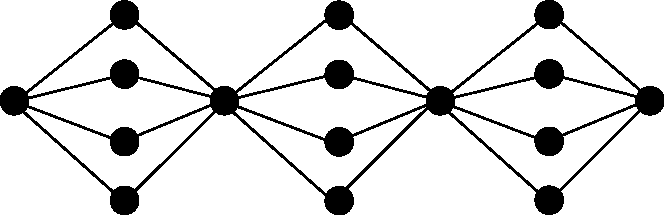
\includegraphics[scale=0.3]{fanout}
\end{center}
To avoid the spurious forking and joining, we {\it delay} the non-determinism
until and unless it is needed in {\it strict contexts} (such as the guard for an
{\tt if}, a called procedure, or a numerical primitive application).
%
Doing so collapses these forks and joins into a linear sequence of states:
\begin{center}

\includegraphics[scale=0.3]{lazy}
\end{center}

This shift does not change the concrete semantics of the language to
be lazy.  Rather, it abstracts over transitions that the original
non-deterministic semantics steps through.
%
We say the abstraction is \emph{lazy} because it delays splitting on
the values in an address until they are \emph{needed} in the
semantics. It does not change the execution order that leads to the
values that are stored in the address.

We introduce a new kind of value,
\spchoice
{$\saddr{\maddr}$}
{$\superposition{\mval{s}}$ (for ``superposition'')},
%
that represents a delayed non-deterministic choice of a value from
\spchoice
{$\msto(\maddr)$}
{$\mval{s}$}.
%
The following rules highlight the changes to the semantics:

\renewcommand{\ext}{\mathit{ext}}

\begin{align*}
\spchoice
{\force &: \Store \times \Value \to \Set(\Value) \\
 \force(\msto,\saddr{\maddr}) &= \msto(\maddr) \\
 \force(\msto,\mval) &= \setof{\mval}}
{\force &: \Value \to \Set(\Value) \\
 \force(\superposition{\mval{s}}) &= \mval{s} \\
 \force(\mval) &= \{\mval\}}
\\
%
\ev{\svar{\mvar},\menv,\mkont,\msto} &\lmachstep\;
\spchoice
{\co{\mkont,\saddr{\menv(\mvar)},\msto}}
{\co{\mkont,\superposition{\msto(\menv(\mvar))},\msto}} \\
%
\co{\kar[^\mcntr_\mlab]{\mexp,\menv,\mkaddr},\mval,\msto}
&\lmachstep\;
\ev[^{\mcntr'}]{\mexp,\menv,\msto',\kfn[^\mcntr_\mlab]{\maddr_f,\mkaddr}} \\
\text{ where }
\maddr_f &= \alloc(\mstate) \\
\msto' &=
\spchoice
{\msto \sqcup[\maddr \mapsto \force(\msto,\mval)]}
{\msto \sqcup[\maddr \mapsto \force(\mval)]} \\
%
\co{\kif[^\mcntr]{\mexpi0,\mexpi1,\menv,\mkaddr},\mval,\msto}
&\lmachstep\;
\ev[^{\mcntr'}]{\mexpi,\menv,\msto,\mkont} \\
\text{ if } \mkont &\in \msto(\mkaddr),
            \strue \in \spchoice{\force(\msto,\mval)}{\force(\mval)}
\end{align*}
Since {\tt if} guards are in strict position, we must force the value
to determine which branch to to take. The middle rule uses $\force$
only to combine with values in the store - it does not introduce
needless non-determinism.

\spchoice{
\noindent
We have two choices for how to implement lazy non-determinism.

\paragraph{Option 1: Lose precision; simplify implementation}
This semantics introduces a subtle precision difference over the
baseline. Consider a configuration where a reference to a variable and
a binding of a variable will happen in one step, since store widening
leads to stepping several states in one big ``step.'' With laziness,
the reference will mean the original binding(s) of the variable or the
new binding, because the actual store lookup is delayed one step
(i.e. laziness is administrative). Without laziness, the reference
will fan out to all the bindings of the variable before the new
binding happens and thus theoretically has an observable precision
difference. % All our benchmarks maintain their precision with lazy non-determinism, however.

\paragraph{Option 2: Regain precision; complicate implementation}
The administrative nature of laziness means that we could remove the
loss in precision by duplicating the reduction relation to specialize
variable lookup. This works since in the semantics of ISWIM with
store-allocated results consumes the value component of states in one
step. This is not the case for semantics that replicate the value
component across reductions, say for popping off exception handler
frames. Further convolution is needed to remove the administrative
nature of laziness in these semantics. Due to the increase of
conceptual and implementation complexity for negligible benefit, we
decided against this approach.

\paragraph{Our choice: option 1}
The configurations that lead to precision loss happen too rarely to
warrant the significant increase in time and memory needed for this
eager non-determinism. Indeed, were the variable reference a step
later and another binding not made in that step, the results of the
two approaches are the same. Without a widened store, lazy
non-determinism is not a complete abstraction with either approach,
but the precision gains are not immediately apparent due to fake
rebinding (a second reference to the same variable chooses a different
value from the first) and other problems. The performance and memory
gains are apparent, so we favor the simplicity over invisible
gains.}{}

\spchoice
{
\begin{theorem}[Soundness]
  If $\mstate \machstep \mstate'$ and $\mstate \sqsubseteq
  \mastate$ then there exists a $\mastate'$ such that $\mastate
  \lmachstep \mastate'$ and $\mstate' \sqsubseteq \mastate'$
\end{theorem}
Here $\sqsubseteq$ is straightforward - the LHS store must be
contained in the RHS store, and if values occur in the states, forcing
the LHS value must be a subset of forcing the corresponding RHS value.
The proof is by cases on $\mstate \machstep \mstate'$.}
{
\begin{theorem}[Completeness]For all $\mexp$,
 $\traces_{\text{Lazy}}(\mexp)$ is a complete abstraction of $\traces_{\text{ISWIM}}(\mexp)$.
\end{theorem}
We have a statement about traces because we need induction to show no
cruft values are in superposition.  The induction hypothesis tells us
that there are non-lazy traces that lead to all the values in
superposition, so when we take a lazy step, we are taking several
non-lazy steps, and we stay in sync. The other direction we just
collapse the superposition in each possibility to construct the
non-lazy traces.}

% Lazy:  cpu time: 32481 real time: 32881 gc time: 547

\subsection{Abstract compilation}

The prior optimization saved time by doing the same amount of
reasoning as before but in fewer transitions. We can exploit the same
idea---same reasoning, fewer transitions---with abstract
compilation. Abstract compilation transforms complex expressions whose
\emph{abstract} evaluation is deterministic into ``abstract
bytecodes.''  The abstract interpreter then does in one transition
what previously took many. In short, abstract compilation eliminates
unnecessary allocation, deallocation and branching. The technique is
precision preserving without store widening. We discuss the precision
differences with store widening at the end of the section.

The following example illustrates
the essence of abstract compilation effect:
\[
\mexp := \sapp{\sapp{\sapp\mvar{\mexp_1}}{\mexp_2}}{\mexp_3}
\]
makes the following transitions:
\begin{align}
& \ev[^\mcntr]{\sapp{\sapp{\sapp\mvar{\mexp_1}}{\mexp_2}}{\mexp_3},\menv,\msto_0,\mkont}\\
\machstep\; &
\ev[^{\mcntr'}]{\sapp{\sapp\mvar{\mexp_1}}{\mexp_2},\menv,\msto_1,\kar{\mexp_3,\menv,\maddr_1}}
\\
\machstep\; &
\ev[^{\mcntr''}]{\sapp\mvar{\mexp_1},\menv,\msto_2,\kar{\mexp_2,\menv,\maddr_2}}
\\
\machstep\; &
\ev[^{\mcntr'''}]{\mvar, \menv,\msto_3,\kar{\mexp_1,\menv,\maddr_3}} % {\mexp_2}
\\
\machstep\; &
\spchoice
{\co{\kar{\mexp_1,\menv,\maddr_3},\saddr{\menv(\mvar)},\msto_4}}
{\co{\kar{\mexp_1,\menv,\maddr_{f3},\maddr_{a3},\maddr_3},\superposition{\msto_4(\menv(\mvar))},\msto_4}}
\end{align}
where \(
\msto_4 = \msto_0 \sqcup [\maddr_1 \mapsto \setof{\mkont},
\maddr_2 \mapsto \setof{\kar{\compile{\mexp_3},\menv,\maddr_1}},
\maddr_3 \mapsto \setof{\kar{\compile{\mexp_2},\menv,\maddr_2}}]\).

Whereas abstract compilation gives us in one step:
\begin{align*}
\compile{\mexp}^\mcntr(\msto_0)(\menv,\epsilon,\mkont) =
\spchoice
{\co{\kar{\compile{\mexp_1},\menv,\maddr_3},\saddr{\menv(\mvar)}},\msdiff_4}
{\co{\kar{\compile{\mexp_1},\menv,\maddr_{f3},\maddr_{a3},\maddr_3},\superposition{\msto'_4(\menv(\mvar))},\msto'_4}}
\end{align*}
where
\begin{equation*}
\msdiff_4 = [\ttuple{\maddr_1}{\setof{\mkont}},
             \ttuple{\maddr_2}{\setof{\kar{\compile{\mexp_3},\menv,\maddr_1}}},
             \ttuple{\maddr_3}{\setof{\kar{\compile{\mexp_2},\menv,\maddr_2}}}]\text.
\end{equation*}

The compilation step converts expressions into functions that expect
the other components of the {\tt ev} state. Its definition in figure
\ref{fig:compile} shows close similarity to the rules for interpreting
{\tt ev} states. The next step is to change reduction rules that
create {\tt ev} states to instead call these functions. Figure
\ref{fig:caam} shows the modified reduction relation. The only change
from the previous semantics is that $\ev{}$ state construction is
replaced by calling the compiled expression. For notational coherence,
we write $\lambda^\mcntr(\mathit{args} \ldots)$ for
$\lambda(\mathit{args} \ldots, \mcntr)$ and
$\mcomp^\mcntr(\mathit{args}\ldots)$ for $\mcomp(\mathit{args}\ldots,
\mcntr)$.

\begin{figure}
\begin{align*}
\compile{\_} &: \Expr \to \Store \\
             &\phantom{: \Expr } \to \Env  \times \StoreDelta \times \Kont \times \Counter \\
             &\phantom{: \Expr } \to \State \\
\mcntr' &= \tick(\mlab,\menv,\msto,\mcntr) \\
\compile{\svar\mvar}_\msto &=
 \lambda^\mcntr(\menv,\msdiff,\mkont) .
\spchoice
{\co{\mkont,\saddr{\menv(\mvar)}},\msdiff}
{\co{\mkont,\superposition{\msto(\menv(\mvar))}},\msdiff}
\\
\compile{\slit\mlit}_\msto &= \lambda^\mcntr(\menv,\msdiff,\mkont) .
\co{\mkont,\mlit},\msdiff
\\
\compile{\slam\mvar\mexp}_\msto &= \lambda^\mcntr(\menv,\msdiff,\mkont) .
\co{\mkont,\clos{\mvar,\compile{\mexp},\menv}},\msdiff
\\
\compile{\sapp[^\mlab]{\mexpi0}{\mexpi1}}_\msto &= \lambda^\mcntr(\menv,\msdiff,\mkont) .
\compile{\mexpi0}^{\mcntr'}(\menv,\msdiff',\kar[_\mlab^\mcntr]{\compile{\mexpi1},\menv,\mkaddr})
\\
&\setlength\arraycolsep{5pt}
\begin{array}{lrl}
\text{ where } & \mkaddr = \allockont^\mcntr_\mlab(\msto,\mkont) \\
               & \msdiff' = \cons{\ttuple{\mkaddr}{\setof{\mkont}}}{\msdiff}
\end{array}
\\
\compile{\sif[^\mlab]{\mexpi0}{\mexpi1}{\mexpi2}}_\msto &= \lambda^\mcntr(\menv,\msdiff,\mkont) .
\compile{\mexpi0}^{\mcntr'}(\menv,\msdiff',\kif[^\mcntr]{\compile{\mexpi1},\compile{\mexpi2},\menv,\maddr})
\\
&\text{ where }\mkaddr = \allockont^\mcntr_\mlab(\msto,\mkont) \\
&\phantom{\text{ where }} \msdiff' = \cons{\ttuple{\mkaddr}{\setof{\mkont}}}{\msdiff}
\end{align*}
\caption{Abstract compilation}
\label{fig:compile}
\end{figure}

\begin{figure}
\begin{gather*}
\begin{align*}
\traces(\mexp) &= \setof{ \inject(\compile{\mexp}^\mtcntr_\bot(\bot,\epsilon,\kmt)) \multimachstep \mstate}
                    \text{ where } \\
\inject(\mastate,\msdiff) &= \wn(\mastate,\replay(\msdiff,\bot)) \\
\wn(\mastate,\msto) \machstep \wn(\mastate',\msto') &\iff \mastate \cmachstep_\msto \mastate',\msdiff \\
\msdiff \text{ is such that } &\replay(\msdiff,\msto) = \msto'
\end{align*}
\\[2mm]
\begin{align*}
%% CONTINUE
\co{\kmt,\mval} &\cmachstep_\msto
\ans{\mval'},\epsilon \text{ if } \mval' \in \spchoice{\force(\msto,\mval)}{\force(\mval)}
\\
\co{\kar[^\mcntr_\mlab]{\mcomp,\menv,\mkaddr},\mval} & \cmachstep_\msto
\mcomp^\mcntr(\msto)(\menv,\msdiff,\kfn[^\mcntr_\mlab]{\maddr_f,\mkaddr}) \\
\text{ where } \maddr_f &= \alloc(\mstate) \\
               \msdiff &= \cons{\ttuple{\maddr_f}{\force(\msto,\mval)}}{\epsilon}
\\
\co{\kfn[^\mcntr_\mlab]{\maddr_f,\mkaddr},\mval} & \cmachstep_\msto
\ap[^\mcntr_\mlab]{\mval,\mval\mkont},\epsilon \\
\text{ if }\mval &\in \msto(\maddr_f), \mkont \in \msto(\mkaddr)
\\
\co{\kif[^\mcntr]{\mcompi0,\mcompi1,\menv,\maddr},\strue} & \cmachstep_\msto
\mcompi{0}^\mcntr(\msto)(\menv,\epsilon,\mkont)
\text{ if }\mkont\in\msto(\maddr)
\\
\co{\kif[^\mcntr]{\mcompi0,\mcompi1,\menv,\maddr},\sfalse} & \cmachstep_\msto
\mcompi{1}^\mcntr(\msto)(\menv,\epsilon,\mkont)
\text{ if }\mkont\in\msto(\maddr)
\\[2mm]
%% APPLY
\ap[^\mcntr_\mlab]{\clos{\mvar,\mcomp,\menv},\mval,\mkont} & \cmachstep_\msto
\mcomp^{\mcntr'}(\msto)(\menv',\msdiff,\mkont) \\
\text{ where }\menv' &= \menv[\mvar\mapsto\maddr] \\
              \msdiff &= \cons{\ttuple{\maddr}{\force(\msto,\mval)}}{\epsilon}
\\
\ap{\mop,\mval,\mkont} & \cmachstep_\msto
\co{\mkont,\mval'},\epsilon \\
\text{ where } \mvalx{u} &\in \spchoice{\force(\msto,\mval)}{\force(\mval)}, \mval'\in\interpdelta(\mop,\mvalx{u})
\end{align*}
\end{gather*}
\caption{Abstract abstract machine for compiled ISWIM}
\label{fig:caam}
\end{figure}

\paragraph{Correctness}
The correctness of abstract compilation seems obvious, but it has
never before been rigorously proved. What constitutes correctness in
the case of dropped states, anyway? Applying an abstract bytecode's
function does many ``steps'' in one go, at the end of which, the two
semantics line up again (modulo representation of expressions). This
constitutes the use of a notion of stuttering. We provide a formal
analysis of abstract compilation \emph{without} store widening with a proof
of a stuttering bisimulation~\cite{ianjohnson:BCG88} between this
semantics and lazy non-determinism without widening to show precision
preservation. %We revisit store widening at the end of the section.

The number of transitions that can occur in succession from an
abstract bytecode is roughly bounded by the amount of expression
nesting in the program. The partial order that defines subexpressions
smaller than the expression in which they occur is well-founded, so we
use this observation to drive our use of a well-founded equivalence
bisimulation (WEB)~\cite{ianjohnson:manolios-diss}. WEBs are equivalent to the notion of a stuttering
bisimulation, but are more amenable to mechanisation (and thus
rigorous proof). They also only require reasoning over one step of the
reduction relation, which makes the proof concise.

We define a refinement from non-compiled to compiled states by
``committing'' all the actions of an $\ev{}$ state (defined similarly to
$\compile{\_}$, but immediately applies the functions), and
subsequently changing all expressions with their compiled
variants. Since WEBs are for single transition systems, a WEB
refinement is over the disjoint union of our two semantics, and the
equivalence relation we use is just that a state is related to its
refined state (and itself). Call this relation $B$.

Before we prove this setup is indeed a WEB, we need one lemma that
applying an abstract bytecode's function is equal to refining the
corresponding $\ev{}$ state:
%
\begin{lemma}[Compile/commit]
Let $\mastate,\msdiff' = \compile{\mexp}^\mcntr_{r(\msto)}(\menv,\msdiff,r(\mkont))$.
Let $\wn(\mastate',\msto') = r(\ev[^\mcntr]{\mexp,\menv,\msto,\mkont})$.
$\wn(\mastate,\replay(\msdiff',\msto)) = \wn(\mastate',\replay(\msdiff,\msto'))$.
\end{lemma}
The proof is by induction on $\mexp$.

\begin{theorem}[Precision preservation]
$B$ is a WEB on $\lmachstep \uplus \machstep$
\end{theorem}

The proof follows by cases on $\lmachstep \uplus \machstep$ with the
WEB \emph{witness} being the well-order on expressions (with a $\bot$
element), and the following $\erankt$, $\erankl$ functions:

\begin{align*}
\erankt(\ev[^\mcntr]{\mexp,\menv,\msto,\mkont}) &= \mexp \\
\erankt(\mstate) &= \bot \quad \text{otherwise} \\
\erankl(s,s') &= 0
\end{align*}
All cases are either simple steps or appeals to the well-order on $\erankt$'s range. The other rank function,
$\erankl$ is unnecessary, so we just make it the constant 0
function. The $\cmachstep$ cases are trivial.

\paragraph{Wide store and abstract compilation}
The fact that many changes happen in one step also makes the
comparison with the widened lazy semantics more subtle. It is possible
for different stores to occur between the different semantics because
abstract compilation can change the order in which the store is
changed. Consider the case where before we might call the same
function from two different places in 3 and 2 steps respectively,
compilation can make that 2 and 1, reversing the order that we bind
values in the store, leading to a mismatch from the previous
semantics. This kind of cross-step store poisoning is inevitable when
a store is shared between several traces. The binding could have just
as easily been observed the other way around in the non-compiled
semantics. Call $\camachstep$ the result of the widening operator from
the previous section on $\cmachstep$.

% Compile: cpu time: 255397 real time: 261532 gc time: 2947

% \noindent
% Compile + Lazy: cpu time: 31173 real time: 31642 gc time: 739

%\newpage

%% Delta Store +k Compile + Lazy:
%%    cpu time: 668 real time: 686 gc time: 41

\subsection{Imperative, preallocated data structures}

Thus far, we have made our optimizations in a purely functional
manner. For the final push for performance, we need to dip into the
imperative. In this section, we show an alternative representation of
the store and seen set that are more space-efficient and are amenable
to destructive updates.

The following transfer function has several components that can be
destructively updated, and intermediate sets can be elided by adding
to global sets. In fact, the log of store deltas can be removed as
well, by updating the store in-place, and on lookup, using the first
value timestamped $\le$ the current timestamp. We start with the
purely functional view.

\subsubsection{Pure setup for imperative implementation}

The store maps to a stack of timestamped sets of abstract values.

\begin{align*}
\msto \in \Store &= \Addr \to \Valstack \\
\mvalstack \in \Valstack &= (\Timestamp \times \wp(\Storeable))^*
\end{align*}

Here we formally define what lookup and update mean at a given
timestamp.

\begin{align*}
\lookup(\mvalstack,t) &=
  \left\{
    \begin{array}{ll}
      \mval{s} & \text{ if } \mvalstack = \cons{\ttuple{t'}{\mval{s}}}{\mvalstack'}, t' \le t \\
      \mval{s'} & \text{ if } \mvalstack = \cons{\ttuple{t'}{\mval{s}}}{\cons{\ttuple{t''}{\mval{s'}}}{\mvalstack'}}, t' > t
    \end{array}\right. \\
\msto \sqcup_t [\maddr \mapsto \mval{s}] &= \msto[\maddr \mapsto \mvalstack],\changep \\
 (\mvalstack,\changep) &= \msto(\maddr)\sqcup_t \mval{s} \\
\epsilon \sqcup_t \mval{s} &= \ttuple{t}{\mval{s}} \\
\cons{\ttuple{t'}{\mval{s}}}{\mvalstack} \sqcup_t \mval{s'} &= \cons{\ttuple{t'}{\mval{s}\sqcup\mval{s'}}}{\mvalstack},\strue \text{ if } t' > t \\
\mvalstack \sqcup_t \mval{s} &= \cons{\ttuple{t+1}{\mval{s^*}}}{\mvalstack},\strue
           \text{ if } \mval{s'} \neq \mval{s^*} \\
 \mval{s'} &= \lookup(\msto(\maddr),t) \\
 \mval{s^*} &= \mval{s} \sqcup \mval{s'} \\
\mvalstack \sqcup_t \mval{s} &= \mvalstack,\sfalse \text{ otherwise}
\end{align*}

For the purposes of space, we reuse the $\cmachstep$ semantics,
although the $\replay$ of the produced $\msdiff$ objects should be
in-place, and the $\lookup$ function should be using this
single-threaded store.  Because the store has all the temporal
information baked into it, we rephrase the core semantics in terms of
a transfer function. The least fixed-point of this function gives a
more compact representation of the reduction relation of the previous
section.

\begin{align*}
\System &= (\widehat{\State} \to {\Timestamp}^*) \times \wp(\widehat{\State}) \times \Store \times \Timestamp \\
{\mathcal F} &: \System \to \System \\
{\mathcal F}(S,F, \msto,t) &= (S',F',\msto', t') \\
\text{ where }
I &= \setof{(\mastate',\msdiff) \mid
       \mastate \in F,
       \mastate \cmachstep_{\msto^*} \mastate',\msdiff} \\
\msto^* &= \lambda \maddr.\lookup(\msto(\maddr),t) \\
\ttuple{\msto'}{\changep} &= \replay(\appendall(\setof{\msdiff \mid (\_,\msdiff) \in I}),\msto) \\
t' &= \left\{\begin{array}{ll} t+1 & \text{ if } \changep \\
              t   & \text{ otherwise}
             \end{array}\right. \\
F' &= \setof{\mastate \mid (\mastate,\_) \in I, \changep \vee S(\mastate) \neq \cons{t}{\_}} \\
S' &= \lambda \mastate. \left\{\begin{array}{ll}
                               \cons{t'}{S(\mastate)} & \text{ if } \mastate \in F' \\
                               S(\mastate) & \text{ otherwise}
                             \end{array}\right.
\end{align*}

We prove semantic equivalence with the previous semantics with a
lock-step bisimulation with the stack of stores abstraction, which
follow from equational reasoning from the following lemmas:

\begin{lemma}
Stores of value stacks completely abstract stacks of stores.
\end{lemma}
This depends on some wellformedness conditions about the order of the
stacks. The store of value stacks can be translated to a stack of
stores by taking successive ``snapshots'' of the store at different
timestamps from the max timestamp it holds down to 0. Vice versa, we
replay the changes across adjacent stores in the stack.

We apply a similar construction to the different representation of seen states in order to get the final result:

\begin{theorem}
${\mathcal F}$ is a complete abstraction of $\camachstep$.
\end{theorem}

\subsubsection{Pure to imperative}

The intermediate data structures of the above transfer function can all be streamlined into globals that are destructively updated. In particular, there are 5 globals:

\begin{enumerate}
\item{$S$: the \emph{seen} set, though made a map for faster membership tests and updates.}
\item{$F$: the \emph{frontier} set, which must be persisent or copied for the iteration through the set to be correct.}
\item{$\msto$: the store, which represents all stores that occur in the machine semantics.}
\item{$t$: the timestamp, or length of the store chain - all stores that occur in the semantics are totally ordered due to single-threading the store.}
\item{$\changep$: whether there has been a store change stepping all states in $F$.}
\end{enumerate}

The reduction relation would then instead of building store deltas,
update the global store. We would also not view it as a general
relation, but a function that adds all next states to $F$ if they have
not already been seen. At the end of iterating through $F$, $S$ is
updated with the new states at the next timestamp.

\subsubsection{Pre-allocating the store}

Internally, the algorithm at this stage uses hash tables to model the store.
%
This is because stores used to be distributed to all states, which
required a compact, dynamic representation.
%
But, such a dynamic structure isn't necessary when we know the
structure of the store in advance: we know all possible entries, and
we know its maximum size.

In a monovariant analysis, the domain of the store is
exactly the set of expressions in the program.
%
If we label each expression with a unique natural, the analysis can
index directly into the store without a hash or a collision.
%
Even for polyvariant analyses, it is possible to compute the maximum
number of addresses and similarly pre-allocate either the spine of the
store or (if memory is no concern) the entire store.

\section{Evaluation}
\label{sec:eval}

We have implemented, optimized, and evaluated an analysis framework
supporting higher-order functions, state, first-class control,
compound data, and a large number of primitive kinds of data and
operations such as floating point, complex, and exact rational
arithmetic.  The analysis is evaluated against a suite of Scheme benchmarks
drawn from the literature.
%
For each benchmark, we collect analysis times, peak memory usage, and
the rate of states-per-second explored by the analysis for each of the
optimizations discussed in section~\ref{sec:opt}, cumulatively
applied.  The analysis is stopped after consuming 30 minutes of time
or 1 gigabyte of space.  When presenting \emph{relative} numbers, we
use the timeout limits as a lower bound on the actual time required,
thus giving a conservative estimate of improvements.

All benchmarks are calculated as an average of 5 runs, done in
parallel, on an 12-core, 64-bit Intel Xeon machine running at 2.40GHz
with 12Gb of memory.

Many benchmarks cause the baseline analyzer to take longer than 30
minutes or to consume more 1 gigabyte of memory, at which point the
analysis is stopped.  This is the case for the largest benchmark
program, {\bf nucleic}, which is 3,500 lines of code and takes under a minute in the
most optimized analyzer.  For those benchmarks that did complete on
the baseline, the optimized analyzer outperformed the baseline by a
factor of two to three orders of magnitude.
% safer to not give exact factors
% 475 to 4,382.

We use the following set of benchmarks:
\begin{figure}
\centering
\begin{tabular}{@{}l|r|r|r|r|r|r|r@{}}
Program & LOC
& \multicolumn{2}{c|}{Time {\small (s)}}
& \multicolumn{2}{c|}{Space {\small (MB)}}
& \multicolumn{2}{c@{}}{Speed {\small (state/s)}}
\\
\hline\hline
nucleic & 3492 & \text{{\small $m$}} & 57.8 & \text{{\small $m$}} & 138 & \text{{\small $m$}} & 7K \\
matrix & 747 & \text{{\small $t$}} & 4.9 & \text{{\small $t$}} & 63 & \text{{\small $t$}} & 68K \\
nbody & 1435 & \text{{\small $t$}} & 38.3 & \text{{\small $t$}} & 124 & \text{{\small $t$}} & 53K \\
earley & 667 & 1.1K & 0.7 & 409 & 60 & 252 & 41K \\
maze & 681 & \text{{\small $t$}} & 4.0 & \text{{\small $t$}} & 60 & \text{{\small $t$}} & 80K \\
church & 42 & 44.9 & 0.2 & 86 & 60 & 714 & 43K \\
lattice & 214 & 348.5 & 0.4 & 231 & 60 & 382 & 72K \\
boyer & 642 & \text{{\small $m$}} & 18.3 & \text{{\small $m$}} & 93 & \text{{\small $m$}} & 33K \\
mbrotZ & 69 & 373.6 & 0.1 & 295 & 60 & 540 & 34K
\end{tabular}

\caption{Overview performance comparison between baseline and
  optimized analyzer (entries of \text{{\small $t$}} mean timeout, and \text{{\small $m$}} mean out of memory).}
\label{fig:bench-overview}
\end{figure}

\begin{enumerate}  %% Maybe use ``dictionary'' style enumeration.

\item {\bf nucleic}: a floating-point intensive application taken from
  molecular biology that has been used widely in benchmarking
  functional language
  implementations~\cite{dvanhorn:Hartel1996Benchmarking} and analyses
  (e.g.~\cite{dvanhorn:wright-jagannathan-toplas98,dvanhorn:jagannathan-etal-popl98}).
  It is a constraint satisfaction algorithm used to determine the
  three-dimensional structure of nucleic acids.

\item {\bf matrix} tests whether a matrix is maximal among all
  matrices of the same dimension obtainable by simple reordering of
  rows and columns and negation of any subset of rows and columns.  It
  is written in continuation-passing style (used in
  \cite{dvanhorn:wright-jagannathan-toplas98,dvanhorn:jagannathan-etal-popl98}).


\item {\bf nbody}: implementation~\cite{ianjohnson:nbody87} of the
  Greengard multipole algorithm for computing gravitational forces on
  point masses distributed uniformly in a cube (used in
  \cite{dvanhorn:wright-jagannathan-toplas98,dvanhorn:jagannathan-etal-popl98}).

\item {\bf earley}: Earley's parsing algorithm, applied to a 15-symbol
  input according to a simple ambiguous grammar.  A real program,
  applied to small data whose exponential behavior leads to a peak
  heap size of half a gigabyte or more during concrete execution.

\item {\bf maze}: generates a random maze using Scheme's {\tt
  call/cc} operation and finds a path solving
  the maze (used in
  \cite{dvanhorn:wright-jagannathan-toplas98,dvanhorn:jagannathan-etal-popl98}).

\item {\bf church}: tests distributivity of multiplication over
  addition for Church numerals (introduced by
  \cite{dvanhorn:Vardoulakis2011CFA2}).

\item {\bf lattice}: enumerates the order-preserving maps between two
  finite lattices (used in
  \cite{dvanhorn:wright-jagannathan-toplas98,dvanhorn:jagannathan-etal-popl98}).

\item {\bf boyer}: a term-rewriting theorem prover (used in
  \cite{dvanhorn:wright-jagannathan-toplas98,dvanhorn:jagannathan-etal-popl98}).

\item {\bf mbrotZ}: generates Mandelbrot set fractal using complex
  numbers.

\item {\bf graphs}: counts the number of directed graphs with a
  distinguished root and \(k\) vertices, each having out-degree at
  most 2. It is written in a continuation-passing style and makes
  extensive use of higher-order procedures---it creates closures
  almost as often as it performs non-tail procedure calls (used by
  \cite{dvanhorn:wright-jagannathan-toplas98,dvanhorn:jagannathan-etal-popl98}).
\end{enumerate}

%% 400 lines for the core, 700 lines for
%% abstraction over optimizations, 1500 lines for primitives and standard
%% list operations, 700 lines for instantiations to different
%% optimizations and 300 for parsing and macro transformers.

Figure~\ref{fig:bench-overview} gives an overview of the benchmark
results in terms of absolute time, space, and speed between the
baseline and most optimized analyzer.  Figure~\ref{fig:bench-all}
plots the factors of improvement over the baseline for each
optimization step. The dip we see in transition rate even though time
taken decreases is to be expected - fewer ``easy'' states are added by
abstract compilation. It increases again with the introduced
algorithmic improvements. Accumulating store changes in addition to
maintaining the store accounts for the higher memory usage when using
the store delta technique without further improvements.

\begin{figure*}
\begin{center}
  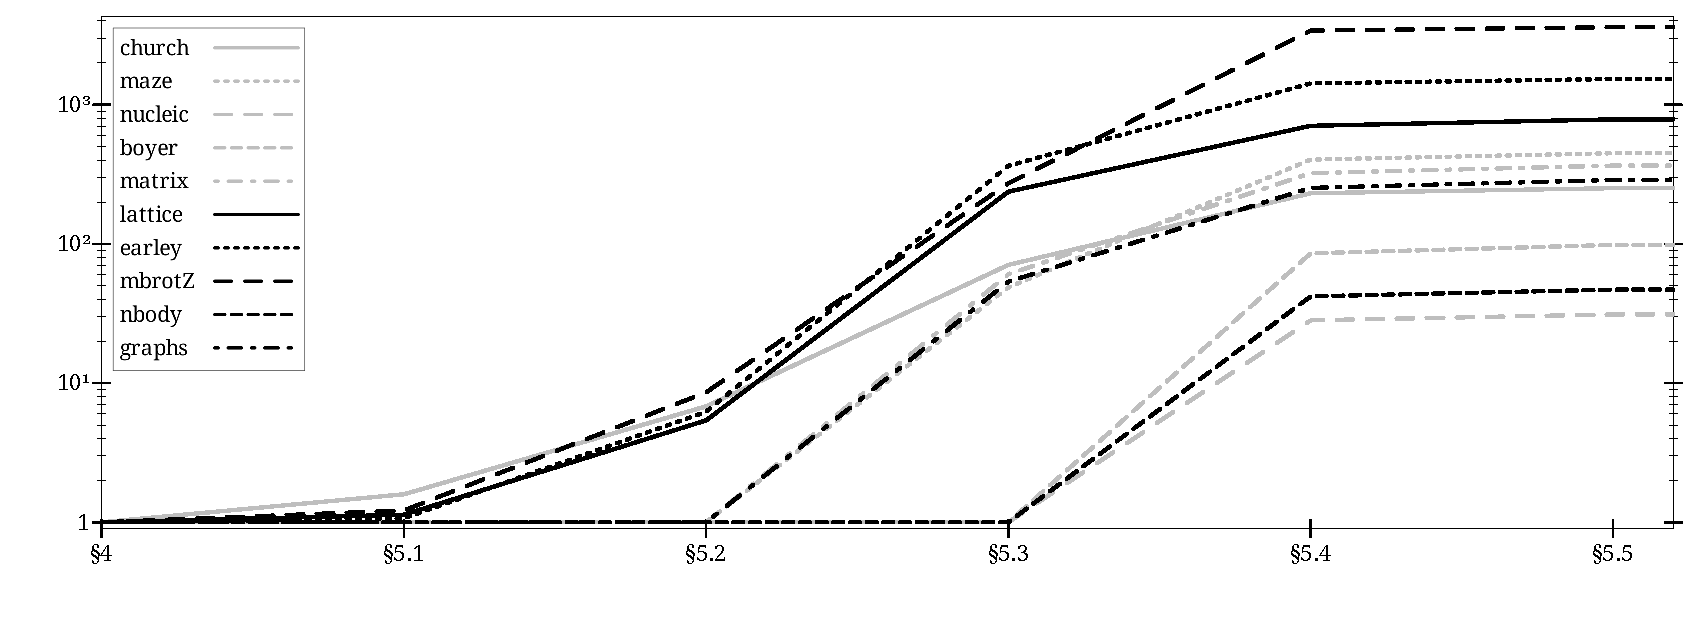
\includegraphics[width=6.5in]{all-relative-time}

  (a) Total analysis time

  \vspace{1em}
  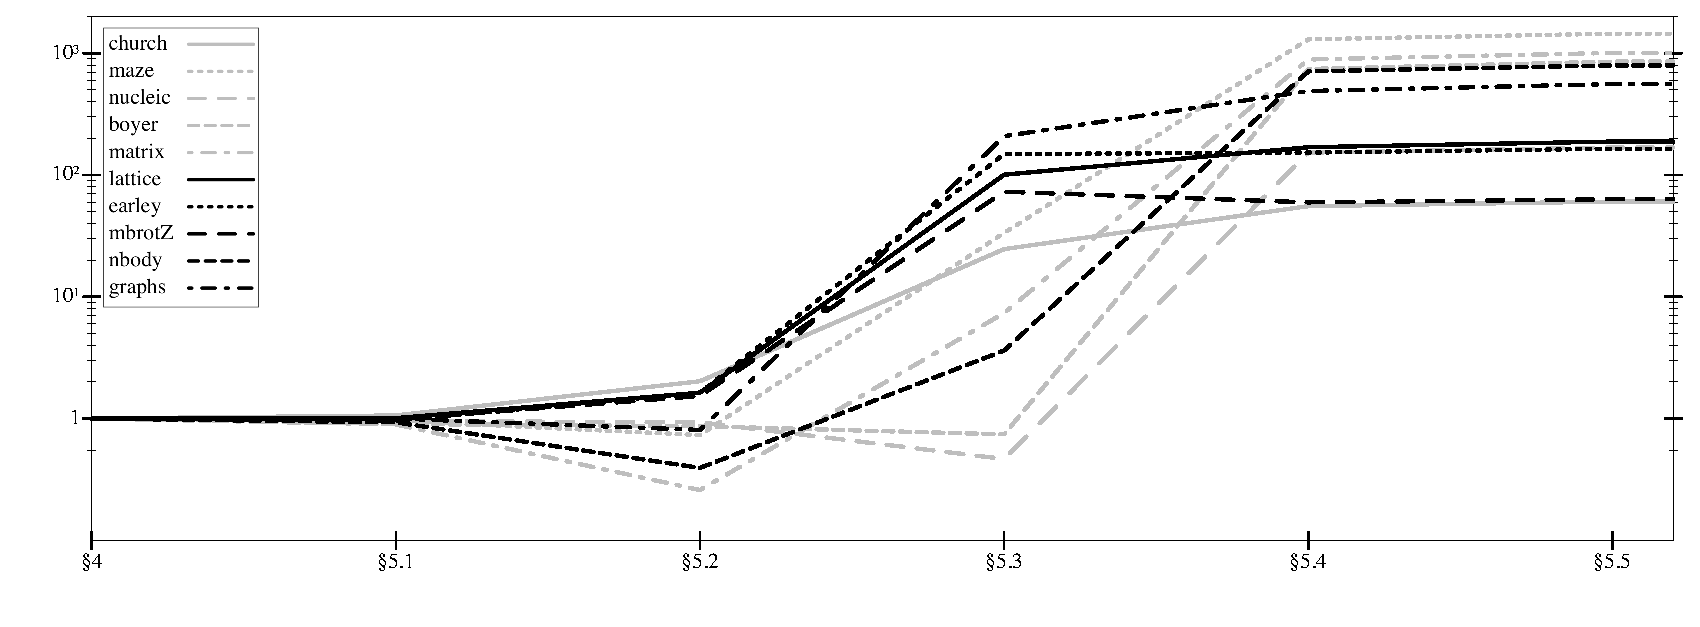
\includegraphics[width=6.5in]{all-relative-speed}

  (b) Rate of state transitions

  \vspace{1em}
  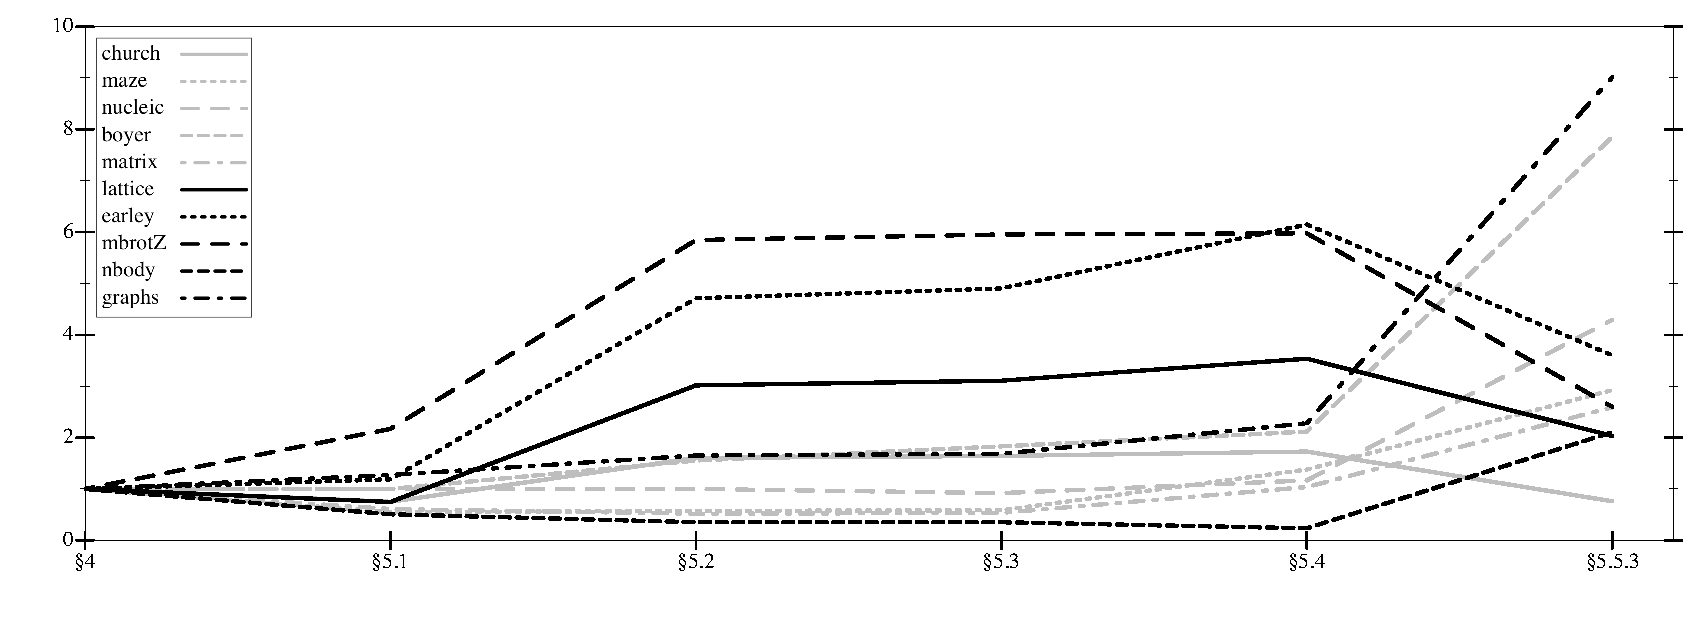
\includegraphics[width=6.5in]{all-relative-space}

  (c) Peak memory usage
\end{center}
\caption{Factors of improvement over baseline for each step of
  optimization (bigger is better).}
\label{fig:bench-all}
\end{figure*}

We evaluated the precision of these techniques with a singleton
variable analysis to find opportunities to inline constants and closed
functions. We found no change in the results across all
implementations, including Shivers' timestamp approximation.

Source code of the implementation and benchmark suite is at:

\begin{center}
\url{https://github.com/dvanhorn/oaam}
\end{center}

\paragraph{Comparison with other flow analysis implementations}

The analysis considered here computes results similar to Earl, et al.'s
0-CFA implementation~\cite{dvanhorn:Earl2012Introspective}, which
times out on the \Church{} benchmark because it does not widen the
store as described for our baseline evaluator.  So even though it
offers a fair point of comparison, a more thorough evaluation is
probably uninformative as the other benchmarks are likely to timeout
as well (and it would require significant effort to extend their
implementation with the features needed to analyze our benchmark
suite).  That implementation is evaluated against much smaller
benchmarks: the largest program is 30 lines.

Vardoulakis and Shivers evaluate their CFA2
analyzer~\cite{dvanhorn:Vardoulakis2011CFA2} against a variant of
0-CFA defined in their framework and the example we draw on is the
largest benchmark Vardoulakis and Shivers consider.  More work would
be required to scale the analyzer to the set of features required by
our benchmarks.

The only analyzers we were able to find that proved capable of
analyzing the full suite of benchmarks considered here were the Soft
Typing system of Wright and
Cartwright~\cite{dvanhorn:Wright1997Practical} and, in many ways its
successor, the Polymorphic splitting system of Wright and
Jagannathan~\cite{dvanhorn:wright-jagannathan-toplas98}.\footnote{This
  is not a coincidence; these papers set a high standard for
  evaluation, which we consciously aimed to approach.}  Unfortunately,
these analyses compute an inherently different and incomparable form
of analysis.  Consequently, we have omitted a complete comparison with
these implementations.  The AAM approach provides more precision in
terms of temporal-ordering of program states, which comes at a cost
that can be avoided in constraint-based approaches.  Consequently
implementation techniques cannot be ``ported'' between these two
approaches.  However, our optimized implementation is within an order
of magnitude of the performance of Wright and Jaganathan's analyzer.
Although we would like to improve this to be more competitive, the
optimized AAM approach still has many strengths to recommend it in
terms of precision, ease of implementation and verification, and rapid
design. We can get closer to their performance by relying on the
representation of addresses and the behavior of $\alloc$ to
pre-allocate most data structures and split the abstract store out
into parts that are more quickly accessed and updated. The first two
of our optimizations can still be applied to an analysis that does
abstract garbage collection~\cite{dvanhorn:Might:2006:GammaCFA},
whereas the polymorphic splitting implementation is tied strongly to a
single-threaded store.

\section{Related work}
\label{sec:related}

\paragraph{Abstracting Abstract Machines}

This work clearly closely follows Van Horn and Might's original papers
on abstracting abstract
machines~\cite{dvanhorn:VanHorn2011Abstracting,dvanhorn:VanHorn2012Systematic},
which in turn is one piece of the large body of research on flow
analysis for higher-order languages (see
Midtgaard~\cite{dvanhorn:Midtgaard2011Controlflow} for a thorough
survey).  The AAM approach sits at the confluence of two major lines
of research: (1) the study of abstract
machines~\cite{dvanhorn:landin-64} and their systematic
construction~\cite{dvanhorn:reynolds-hosc98}, and (2) the theory of
abstract interpretation
\cite{dvanhorn:Cousot:1977:AI,dvanhorn:Cousot1979Systematic}.


\paragraph{Frameworks for flow analysis of higher-order programs}

Besides the original AAM work, the analysis most similar to that
presented in section~\ref{sec:aam} is the infinitary control-flow
analysis of Nielson and Nielson~\cite{dvanhorn:nielson-nielson-popl97}
and the unified treatment of flow analysis by Jagannathan and
Weeks~\cite{dvanhorn:jagannathan-weeks-popl95}.  Both are
parameterized in such a way that in the limit, the analysis is
equivalent to an interpreter for the language, just as is the case
here.  What is different is that both give a constraint-based
formulation of the abstract semantics rather than a finite machine
model.

\paragraph{Abstract compilation}

Boucher and Feeley \cite{dvanhorn:Boucher1996Abstract} introduced the
idea of abstract compilation, which used closure generation
\cite{dvanhorn:Feeley1987Using} to improve the performance of control
flow analysis.  We have adapted the closure generation technique from
compositional evaluators to abstract machines and applied it to similar
effect.

\paragraph{Constraint-based program analysis for higher-order languages}

Constraint-based program analyses
(e.g.~\cite{dvanhorn:nielson-nielson-popl97,dvanhorn:wright-jagannathan-toplas98,dvanhorn:Meunier2006Modular,dvanhorn:steckler-wand-toplas97})
typically compute sets of abstract values for each program point.
These values approximate values arising at run-time for each
program point.  Value sets are computed as the least solution to a set
of (inclusion or equality) constraints.  The
constraints must be designed and proved as a sound approximation of
the semantics.  Efficient implementations of these kinds of analyses
often take the form of worklist-based graph algorithms for constraint
solving, and are thus quite different from the interpreter
implementation.  The approach thus requires effort in constraint
system design and implementation, and the resulting system require
verification effort to prove the constraint system is sound and that
the implementation is correct.

This effort increases substantially as the complexity of the analyzed
language increases.  Both the work of maintaining the concrete
semantics and constraint system (and the relations between them) must
be scaled simultaneously.  However, constraint systems, which have
been extensively studied in their own right, enjoy efficient
implementation techniques and can be expressed in declarative logic
languages that are heavily
optimized~\cite{dvanhorn:bravenboer-smaragdakis-oopsla09}.
Consequently, constraint-based analyses can be computed quickly.  For
example, Jagannathan and Wright's polymorphic splitting
implementation~\cite{dvanhorn:wright-jagannathan-toplas98} analyses
the \Church{} benchmark about 25 times faster than the fastest
implementation considered here.  These analyses compute very different
things, so the performance comparison is not apples-to-apples.

The AAM approach, and the state transition graphs it generates, encodes
temporal properties not found in classical constraint-based analyses
for higher-order programs.
%
Such analyses (ultimately) compute judgments on program terms and
contexts, e.g., at expression $e$, variable $x$ may have value $v$.
%
The judgments do not relate the order in which expressions and context
may be evaluated in a program, e.g., it has nothing
to say with regard to question like, ``Do we always evaluate $e_1$
before $e_2$?'' or ``Is it always the case that a file handle is
opened, read and then closed in that order?''
%
The state transition graphs can answer these kinds of queries, but
this does not come for free: respecting temporal order imposes an
order in which states and terms may be evaluated \emph{during} the
analysis.

\section{Conclusion}
\label{sec:conclusion}

Abstract machines are not only a good model for rapid analysis
development, they can be systematically developed into efficient
algorithms that can be proved correct. We view the primary
contribution of this work as a systematic path that eases the design,
verification, and implementation of analyses using the abstracting
abstract machine approach to within a factor of performant
constraint-based analyses.

%% \acks Sam Tobin-Hochstadt for encouragement and feedback -- he was
%% the first to prompt us to look into how make effective
%% implementations of the AAM approach.

%% Vincent St Amour and Mitchell Wand for feedback on early drafts.
%% Greg Morrisset and Matthias Felleisen for discussions.

%% NSF, DARPA


\paragraph{Acknowledgments}

We thank Suresh Jagannathan for providing source code to the
polymorphic splitting
analyzer~\cite{dvanhorn:wright-jagannathan-toplas98} and Ilya Sergey
for the introspective pushdown
analyzer~\cite{dvanhorn:Earl2012Introspective}.


\balance
\bibliographystyle{plain}
%\documentclass[preprint,onecolumn,9pt]{sigplanconf} %{onecol}
\usepackage{alltt,mathpartir}
\usepackage{amsmath,amsthm}
\usepackage{amssymb}
\usepackage{stmaryrd}
\usepackage{url}
\usepackage{graphicx}
\usepackage{balance}
\usepackage{calc}

\newtheorem{theorem}{Theorem}
\newtheorem{lemma}{Lemma}

\newcommand{\naive}{naive}
\newcommand{\naively}{naively}
\newcommand{\Naive}{Naive}
\newcommand{\Naively}{Naively}
% \usepackage{xltxtra}
% \setmonofont[Scale=MatchLowercase]{DejaVu Sans Mono}
%
\input{preamble}

\begin{document}

\conferenceinfo{WXYZ '05}{date, City.}
\copyrightyear{2005}
\copyrightdata{[to be supplied]}

% \titlebanner{banner above paper title}        % These are ignored unless
% \preprintfooter{short description of paper}   % 'preprint' option specified.

%\title{Provably Correct, Low-Cost Optimizations for Abstract Abstract Machines}
\title{Correctly Optimizing Abstract Abstract Machines}

\authorinfo{J. Ian Johnson \and Nicholas Labich \and Matthew Might \and David Van Horn}
           {}
           {}
%% \authorinfo{J. Ian Johnson}
%%            {Northeastern University}
%%            {ianj@ccs.neu.edu}
%% \authorinfo{Nicholas Labich}
%%            {Northeastern University}
%%            {labichn@ccs.neu.edu}
%% \authorinfo{Matthew Might}
%%            {University of Utah}
%%            {might@cs.utah.edu}
%% \authorinfo{David Van Horn}
%%            {Northeastern University}
%%            {dvanhorn@ccs.neu.edu}
\maketitle

\begin{abstract}
The technique of \emph{abstracting abstract machines} (AAM) provides a
systematic approach for deriving computable approximations of
evaluators that are easily proved sound.
%
This article contributes a complementary step-by-step process for
subsequently going from a \naive{} analyzer derived under the AAM
approach, to an efficient and correct implementation.  The end result
of the process is a two to three order-of-magnitude improvement over
the systematically derived analyzer, making it competitive with
hand-optimized implementations that compute fundamentally less precise
results.
\end{abstract}

%% \category{CR-number}{subcategory}{third-level}

%% \terms
%% term1, term2

%% \keywords
%% keyword1, keyword2

\section{Introduction}

Program analysis provides sound predictive models of program behavior, but
in order for such models to be effective, they must be efficiently
computable and correct.  Past approaches to designing program analysis
have often featured abstractions that are far removed from the
original language semantics, requiring ingenuity in their construction
and effort in their verification.
%
The \emph{abstracting abstract machines} (AAM)
approach~\cite{dvanhorn:VanHorn2011Abstracting,dvanhorn:VanHorn2012Systematic}
to deriving program analyses provides an alternative: a systematic way
of transforming a programming language semantics in the form of an
abstract machine into a family of abstract interpreters.  It thus reduces
the burden of constructing and verifying the soundness of an abstract
interpreter.
%

%
% Specifically, these policies tune precision for control,
% the environment, the store, and base value domains.

By taking a
machine-oriented view of computation, AAM makes it possible to design,
verify, and implement program analyzers for realistic language
features typically considered difficult to model.  The approach was
originally applied to features such as higher-order functions,
stack inspection, exceptions, laziness, first-class continuations, and
garbage collection.  It has since been used to verify actor-
\cite{local:DOsualdo:12A} and
thread-based~\cite{dvanhorn:Might2011Family} parallelism and
behavioral contracts~\cite{dvanhorn:TobinHochstadt2012Higherorder}; it
has been used to model Coq~\cite{local:harvard},
Dalvik~\cite{local:dalvik}, Erlang~\cite{local:DOsualdo:12B},
JavaScript~\cite{local:DBLP:journals/corr/abs-1109-4467}, and
Racket~\cite{dvanhorn:TobinHochstadt2012Higherorder}.

The primary strength of the approach is that abstract interpreters can
be easily derived through a small number of steps from existing
machine models.  Since the relationships between abstract machines and
higher-level semantic models---such as definitional
interpreters~\cite{dvanhorn:reynolds-hosc98}, structured operational
semantics~\cite{dvanhorn:Plotkin1981Structural}, and reduction
semantics~\cite{dvanhorn:Felleisen2009Semantics}---are well
understood~\cite{dvanhorn:Danvy:DSc}, it is possible to navigate from
these high-level semantic models to sound program analyzers in a
systematic way.  Moreover, since these analyses so closely resemble a
language's interpreter (a) implementing an analysis requires little
more than implementing an interpreter, (b) a single implementation can
serve as both an interpreter and analyzer, and (c) verifying the
correctness of the implementation is straightforward.

Unfortunately, the AAM approach yields analyzers with poor performance
relative to hand-optimized analyzers.
%
Our work takes aim squarely at this ``efficiency gap,'' and narrows it
in an equally systematic way through a number of simple steps, many of
which are inspired by run-time implementation techniques such as
laziness and compilation to avoid interpretative overhead.  Each of
these steps is proven correct, so the end result is an implementation
that is trustworthy and efficient.

In this article, we develop a systematic approach to deriving a
practical implementation of an abstract-machine-based analyzer using
mostly semantic means rather than tricky engineering. Our goal is to
empower programming language implementers and researchers to explore
and convincingly exhibit their ideas with a low barrier to entry. The
optimizations we describe are widely applicable and apparently
effective to scale far beyond the size of programs typically considered
in the recent literature on flow analysis for functional languages.

\section{At a glance}

\begin{figure}[t]
\begin{center}
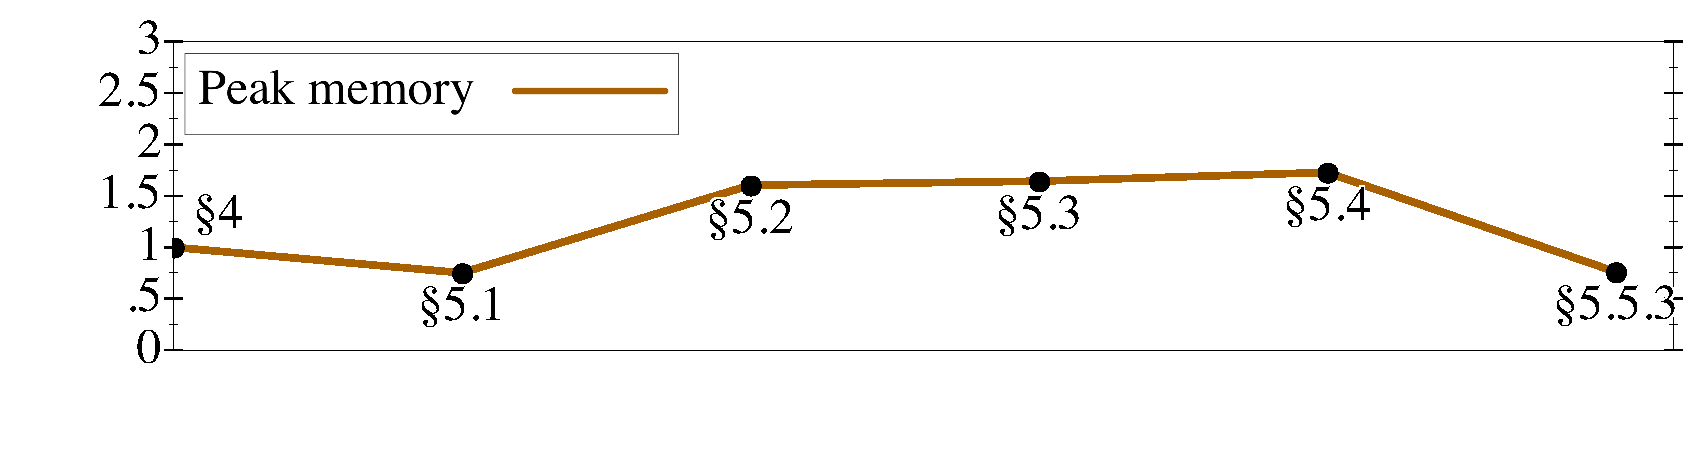
\includegraphics[width=3.2in]{church-relative-space}
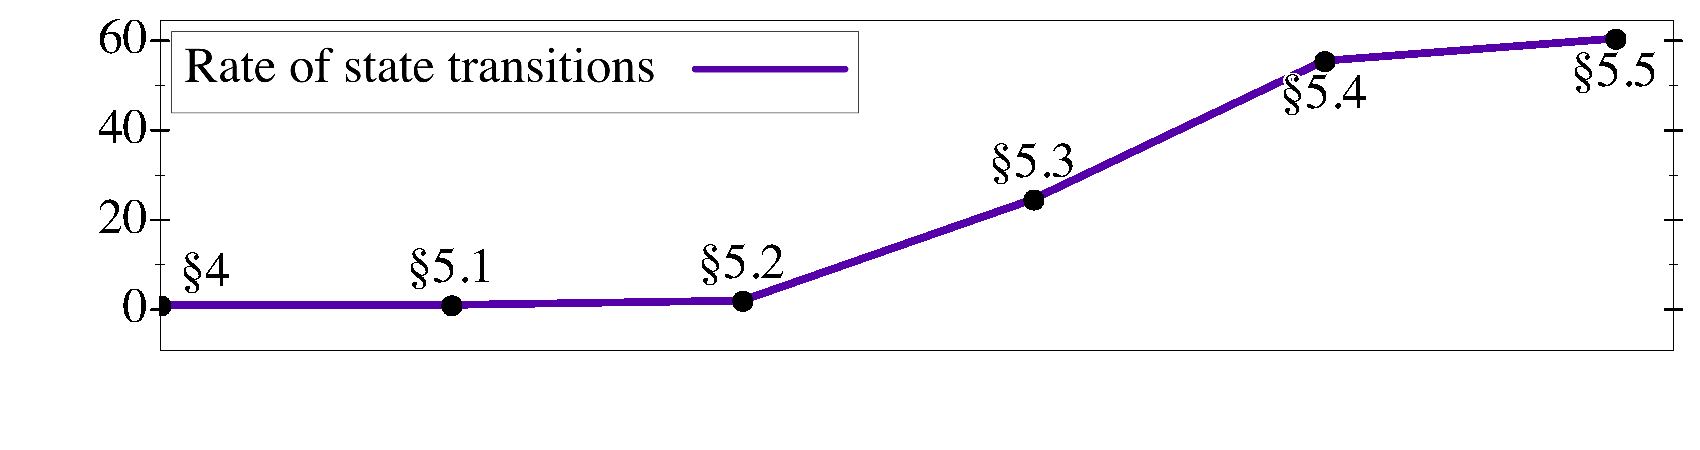
\includegraphics[width=3.2in]{church-relative-speed}
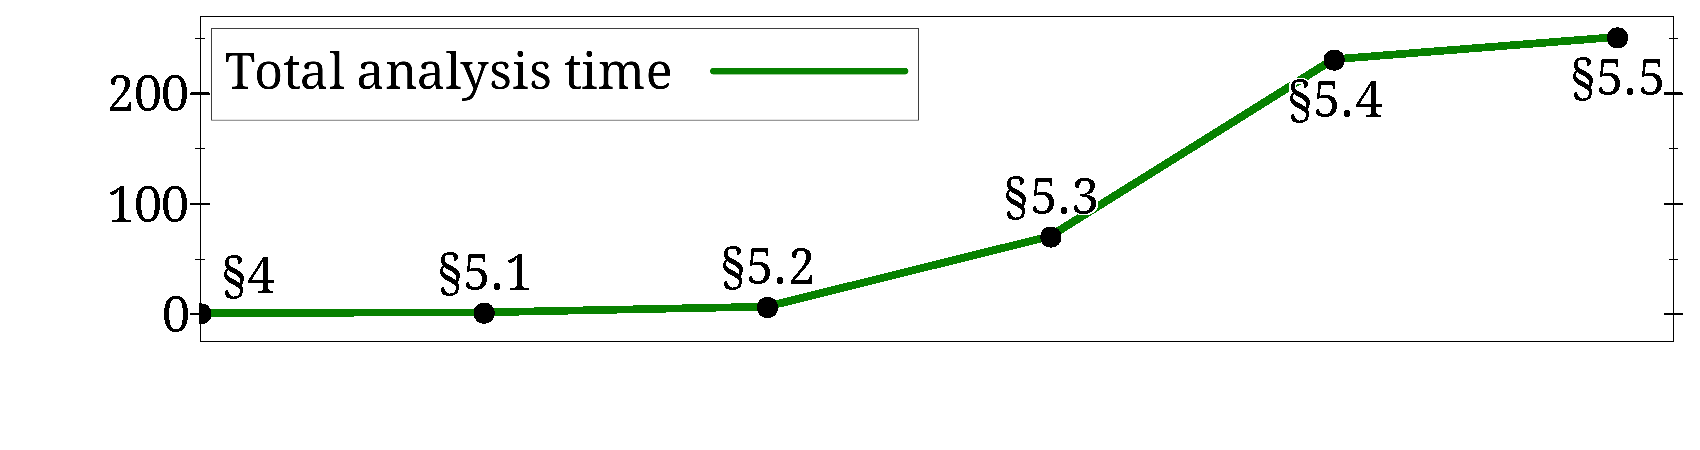
\includegraphics[width=3.2in]{church-relative-time}
\vspace{-1.5em}
\end{center}
\caption{Factor improvements over the baseline analyzer for the
  \Church{} benchmark in terms of peak memory usage, the rate of state
  transitions, and total analysis time. (Bigger is better.) Each point
  is marked with the section that introduces the optimization.}
\label{fig:churchtime}
\end{figure}


We start with a quick review of the AAM approach to develop an
analysis framework and then apply our step-by-step optimization
techniques in the simplified setting of a core functional language.
This allows us to explicate the optimizations with a minimal amount of
inessential technical overhead.  Following that, we scale this
approach up to an analyzer for a realistic untyped, higher-order
imperative language with a number of interesting features and then
measure improvements across a suite of benchmarks.

At each step during the initial presentation and development, we
evaluated the implementation on a set of benchmarks. The highlighted
benchmark in figure \ref{fig:churchtime} is from Vardoulakis and
Shivers~\cite{dvanhorn:Vardoulakis2011CFA2} that tests distributivity
of multiplication over addition on Church numerals.  For the
step-by-step development, this benchmark is particularly informative:
\begin{enumerate}
\item it can be written in most modern programming languages,
%
\item it was designed to stress an analyzer's ability to deal with
  complicated environment and control structure arising from the use
  of higher-order functions to encode arithmetic, and
%
\item its improvement is about median in the benchmark suite
  considered in section~\ref{sec:eval}, and thus it serves as a good
  sanity check for each of the optimization techniques considered.
\end{enumerate}

We start, in section~\ref{sec:aam}, by developing an abstract
interpreter according to the AAM approach.  In the initial
abstraction, each state carries a store (what is called per-state
store variance). The space of stores is exponential in size; without
further abstraction, the analysis is exponential and thus cannot
analyze the example in a reasonable amount of time.  In
section~\ref{sec:baseline}, we perform a further abstraction by
widening the store.  The resulting analyzer sacrifices precision for
speed and is able to analyze the example in about 1 minute.  This step
is described by Van Horn and Might~\cite[\S
3.5--6]{dvanhorn:VanHorn2012Systematic} and is necessary to make even
small examples feasible.  We therefore take a widened interpreter as
the baseline for our evaluation.

Section~\ref{sec:opt} gives a series of simple abstractions and
implementation techniques that, in total, speed up the analysis by
nearly a factor of 500, dropping the analysis time to a fraction of a
second.  Figure~\ref{fig:churchtime} shows the step-wise improvement
of the analysis time for this example.

\begin{figure}[t]
\begin{center}
\begin{tabular}{ccc}
\raisebox{1ex-\height}{
\includegraphics[height=3.5in]{introspective-base.pdf}}
&
\raisebox{1ex-\height}{
\includegraphics[height=3.5in]{introspective-lazy.pdf}}
&
\raisebox{1ex-\height}{
\includegraphics[height=3in]{introspective-lazyc.pdf}}
\\
(a) Baseline
&
(b) Lazy
&
(c) Compiled (\& lazy)
\end{tabular}
\end{center}
\caption{Example state graphs for the program above.  Part (a) shows
  the result of the baseline analyzer.  It has long ``corridor''
  transitions and ``diamond'' subgraphs that fan-out from
  nondeterminism and fan-in from joins.  Part (b) shows the result of
  performing nondeterminism lazily and thus avoids many of the diamond
  subgraphs.  Part (c) shows the result of abstract compilation that
  removes interpretive overhead in the form of intermediate states,
  thus minimizing the corridor transitions.  The end result is a more
  compact abstraction of the program that can be generated faster.}
\label{fig:state-graphs}
\end{figure}

The AAM approach, in essence, does the following: it takes a
machine-based view of computation and turns it into a \emph{finitary
  approximation} by bounding the size of the store.  With a limited
address space, the store must map addresses to \emph{sets} of values.
Store updates are interpreted as joins, and store dereferences are
interpreted by non-deterministic choice of an element from a set.  The
result of analyzing a program is a finite directed graph where nodes
in the graph are (abstract) machine states and edges denote machine
transitions between states.

The techniques we propose for optimizing analysis fall into the
following categories:
\begin{enumerate}
\item generate fewer states by avoiding the eager exploration of
  non-deterministic choices that will later collapse into a single
  join point.  We accomplish this by applying lazy evaluation
  techniques so that non-determinism is evaluated \emph{by need}.

\item generate fewer states by avoiding unnecessary, intermediate
  states of a computation.  We accomplish this by applying compilation
  techniques from functional languages to avoid interpretive overhead
  in the machine transition system.

\item generate states faster.  We accomplish this by better algorithm
  design in the fixed-point computation we use to generate state graphs.
\end{enumerate}
Figure~\ref{fig:state-graphs} shows the effect of (1) and (2) for a
small example due to Earl, et
al.~\cite{dvanhorn:Earl2012Introspective}.
By generating significantly fewer states at a significantly faster
rate, we are able to achieve large performance improvements in terms
of both time and space.

Section~\ref{sec:eval} describes the evaluation of each optimization
technique applied to an implementation supporting a more realistic set
of features, including mutation, first-class control, compound data, a
full numeric tower and many more forms of primitive data and
operations.
%
We evaluate this implementation against a set of benchmark programs
drawn from the literature.
%
For all benchmarks, the optimized analyzer outperforms the baseline
by at least a factor of
% 475
two to
% 4,382
three orders of magnitude.

Section~\ref{sec:related} relates this work to the literature and
section~\ref{sec:conclusion} concludes.

%\newpage
\section{Abstract interpretation of ISWIM}
\label{sec:aam}

In this section, we give a brief review of the AAM approach by
defining a sound analytic framework for a core higher-order functional
language: Landin's ISWIM~\cite{dvanhorn:Landin1966Next}.  In the
subsequent sections, we will explore optimizations for the analyzer in
this simplified setting, but scaling these techniques to realistic
languages is straightforward and has been done for the analyzer
evaluated in section~\ref{sec:eval}.

ISWIM is a family of programming languages parameterized by a set of
base values and operations.  To make things concrete, we consider a
member of the ISWIM family with integers, booleans, and a few
operations.
%
Figure~\ref{fig:syntax} defines the syntax of ISWIM.  It
includes variables, literals (either integers, booleans, or
operations), $\lambda$-expressions for defining procedures, procedure
applications, and conditionals.  Expressions carry a label, $\mlab$,
which is drawn from an unspecified set and denotes the source location
of the expression; labels are used to disambiguate distinct, but
syntactically identical pieces of syntax.  We omit the label
annotation in contexts where it is irrelevant.

\begin{figure}
\[
\begin{array}{l@{\qquad}rcl}
\text{Expressions} & \mexp &=& \svar[^\mlab]\mvar\\
&&|& \slit[^\mlab]\mlit\\
&&|& \slam[^\mlab]\mvar\mexp\\
&&|& \sapp[^\mlab]\mexp\mexp \\
&&|& \sif[^\mlab]\mexp\mexp\mexp \\
\text{Variables}&\mvar &=& \syntax{x}\ |\ \syntax{y}\ |\ \dots\\
\text{Literals}&\mlit &=& \mnum\ |\ \mbln\ |\ \mop\\
\text{Integers}&\mnum &=& \syntax{0}\ |\ \syntax{1}\ |\ \syntax{-1}\ |\ \dots\\
\text{Booleans}&\mbln &=& \strue\ |\ \sfalse\\
\text{Operations}&\mop &=& \syntax{zero?}\ |\ \syntax{add1}\ |\ \syntax{sub1}\ |\ \dots
\end{array}
\]
\caption{Syntax of ISWIM}
\label{fig:syntax}
\end{figure}

\begin{figure}
\[
\begin{array}{l@{\qquad}rcl}
\text{Values} & \mval,\mvalx{u} &=& \clos{\mvar,\mexp,\menv}\ |\ \mlit\ |\ \mkont\\
\text{States} & \mstate &=& \ev{\mexp,\menv,\msto,\mkont}\\
                       &&|& \co{\mkont,\mval,\msto}\\
                       &&|& \ap{\mval,\mval,\msto,\mkont}\\
\text{Continuations} & \mkont &=& \kmt\\
&&|& \kfn{\mval,\mkaddr}\\
&&|& \kar{\mexp,\menv,\mkaddr}\\
&&|& \kif{\mexp,\mexp,\menv,\mkaddr}\\
\text{Addresses} &\maddr&\in&\Addr \\
\text{Environments} &\menv&\in& \Var \rightharpoonup \Addr\\
\text{Stores} &\msto&\in& \Addr \rightharpoonup \mathcal{P}(\Value)
\end{array}
\]
\caption{Abstract machine components}
\label{fig:domains}
\end{figure}


The semantics are defined in terms of a machine model.  The machine
components are defined in figure~\ref{fig:domains};
figure~\ref{fig:aam} defines the transition relation.  The evaluation
of a program is defined as its set of traces that arise from iterating the
machine transition relation.  The
machine is a very slight variation on a standard abstract machine for
ISWIM in ``eval, continue, apply'' form~\cite{dvanhorn:Danvy:DSc}.  It
can be systematically derived from a definitional interpreter through
a continuation-passing style transformation and defunctionalization,
or from a structural operational semantics using the refocusing
construction of Danvy and
Nielsen~\cite{dvanhorn:Danvy-Nielsen:RS-04-26}.

Compared with the standard machine semantics, this definition is
different in the following ways, which make it abstractable as a
program analyzer:
\begin{itemize}
\item the store maps addresses to \emph{sets} of values,\footnote{
More generally, we can have stores map to any domain that forms
 a Galois connection with values, enabling $\interpdelta$ to
produce elaborate abstractions of base values (e.g., interval or octagon
abstractions). We use sets of values for a simpler exposition.
} not
  single values,

\item continuations are heap-allocated, not stack-allocated,
\item there are ``timestamps'' ($\mcntr \in \Counter$) and syntax
  labels ($\mlab$) threaded through the computation, and
\item the machine is implicitly parameterized by the functions
  $\alloc$, $\allockont$, $\tick$, $\interpdelta$, and spaces
  $\Addr$, $\Counter$ (and initial $\mcntr_0 \in \Counter$).
\end{itemize}


\begin{figure}
\begin{gather*}
\begin{align*}
\traces(\mexp) &= \{ \ev[^{\mtcntr}]{\mexp,\varnothing,\varnothing,\kmt} \multimachstep \mstate \} \text{ where }
\end{align*}
\\[2mm]
\begin{array}{@{}r@{\ }c@{\ }l@{}}
\mstate &\machstep&\mstate' \text{ defined to be the following} \\
&&\text{let } \mcntr' =\tick(\mstate) \\
%% EVAL
\ev{\svar\mvar,\menv,\msto,\mkont} &\machstep&
\co{\mkont,\mval,\msto}
\text{ if }\mval \in \msto(\menv(\mvar))
\\
\ev{\slit\mlit,\menv,\msto,\mkont} &\machstep&
\co{\mkont,\mlit,\msto}
\\
\ev[^\mcntr]{\slam\mvar\mexp,\menv,\msto,\mkont} &\machstep&
\co[^{\mcntr'}]{\mkont,\clos{\mvar,\mexp,\menv},\msto}
\\
\ev[^\mcntr]{\sapp[^\mlab]{\mexpi0}{\mexpi1},\menv,\msto,\mkont} &\machstep&
\ev[^{\mcntr'}]{\mexpi{0},\menv,\msto',\kar[_\mlab^\mcntr]{\mexpi{1},\menv,\mkaddr}}
\\
&&
\text{ where }\mkaddr = \allockont^\mcntr_\mlab(\msto,\mkont) \\
&&\phantom{\text{ where }}\msto' = \msto\sqcup[\mkaddr \mapsto \setof{\mkont}]
\\
\ev[^\mcntr]{\sif[^\mlab]{\mexpi0}{\mexpi1}{\mexpi2},\menv,\msto,\mkont} &\machstep&
\ev[^{\mcntr'}]{\mexpi0,\menv,\msto',\kif[^\mcntr]{\mexpi1,\mexpi2,\menv,\mkaddr}}
\\
&&
\text{ where }\mkaddr = \allockont^\mcntr_\mlab(\msto,\mkont) \\
&&\phantom{\text{ where }}\msto' = \msto\sqcup[\mkaddr \mapsto \setof{\mkont}]
\\[2mm]
%% CONTINUE
\co{\kmt,\mval,\msto} &\machstep&
\ans{\msto,\mval}
\\
\co{\kar[^\mcntr_\mlab]{\mexp,\menv,\mkaddr},\mval,\msto} & \machstep&
\ev[^\mcntr]{\mexp,\menv,\msto,\kfn[^\mcntr_\mlab]{\mval,\mkaddr}}
\\
\co{\kfn[^\mcntr_\mlab]{{\mvalx{u}},\mkaddr},\mval,\msto} & \machstep&
\ap[^\mcntr_\mlab]{\mvalx{u},\mval,\mkont,\msto}
\text{ if }\mkont \in \msto(\mkaddr)
\\
\co{\kif[^\mcntr]{\mexpi0,\mexpi1,\menv,\mkaddr},\strue,\msto} & \machstep&
\ev[^{\mcntr'}]{\mexpi0,\menv,\msto,\mkont}
\text{ if }\mkont\in\msto(\mkaddr)
\\
\co{\kif[^\mcntr]{\mexpi0,\mexpi1,\menv,\mkaddr},\sfalse,\msto} & \machstep&
\ev[^{\mcntr'}]{\mexpi1,\menv,\msto,\mkont}
\text{ if }\mkont\in\msto(\mkaddr)
\\[2mm]
%% APPLY
\ap[^\mcntr_\mlab]{\clos{\mvar,\mexp,\menv},\mval,\msto,\mkont} & \machstep&
\ev[^{\mcntr'}\!]{\mexp,\menv',\msto',\mkont}
\\
&&\text{ where } \maddr  =\alloc(\mstate) \\
&&\phantom{\text{ where }} \menv' = \menv[\mvar\mapsto\maddr] \\
&&\phantom{\text{ where }} \msto' = \msto\sqcup[\maddr\mapsto\{\mval\}] \\
\\
\ap[^\mcntr_\mlab]{\mop,\mval,\msto,\mkont} & \machstep&
\co{\mkont,\mval',\msto}
\text{ if } \mval'\in\interpdelta(\mop,\mval)
\end{array}
\end{gather*}
\caption{Abstract abstract machine for ISWIM}
\label{fig:aam}
\end{figure}


\paragraph{Concrete interpretation} To characterize concrete interpretation, set the implicit
parameters of the relation given in figure~\ref{fig:aam} as follows:
\begin{align*}
\alloc(\mstate) &= \maddr \mbox{ where } \maddr \notin \text{ the } \msto \text{ within } \mstate \\
\allockont^\mcntr_\mlab(\msto,\mkont) &=\mkaddr \mbox{ where } \mkaddr \notin \msto
\end{align*}
These functions appear to ignore $\mlab$ and $\mcntr$, but they can be
used to determinize the choice of fresh addresses. The $\sqcup$ on
stores in the figure is a point-wise lifting of $\cup$: $\msto \sqcup \msto' =
\lambda \maddr. \msto(\maddr) \cup \msto'(\maddr)$. The resulting
relation is non-deterministic in its choice of addresses, however it
must always choose a fresh address when allocating a continuation or
variable binding.  If we consider machine states equivalent up to
consistent renaming and fix an allocation scheme, this relation
defines a deterministic machine (the relation is really a function).

The interpretation of primitive operations is defined by setting
$\interpdelta$ as follows:
\begin{align*}
\mnum+1 &\in \interpdelta(\saddone,\mnum) &
\mnum-1 &\in \interpdelta(\ssubone,\mnum)\\
\strue &\in \interpdelta(\szerohuh,\szero) &
\sfalse &\in \interpdelta(\szerohuh,\mnum)\text{ if }\mnum\neq \szero\\
\end{align*}


\paragraph{Abstract interpretation} To characterize abstract
interpretation, set the implicit parameters just as above, but drop
the $\maddr \not\in \msto$ condition. The $\interpdelta$ relation takes some care
to not make the analysis run forever; a simple instantiation is a flat
abstraction where arithmetic operations return an abstract top element
$\sNum$, and $\szerohuh$ returns both $\strue$ and $\sfalse$ on
$\sNum$.  This family of interpreters is also non-deterministic in
choices of addresses, but it is free to choose addresses that are
already in use.  Consequently, the machines may be non-deterministic
when multiple values reside in a store location.

It is important to recognize from this definition that \emph{any}
allocation strategy is a sound abstract
interpretation~\cite{dvanhorn:Might2009Posteriori}.  In particular,
concrete interpretation is a kind of abstract interpretation.  So is
an interpretation that allocates a single cell into which all bindings
and continuations are stored.  The former is an abstract
interpretation that is non-computable and gives only the ground truth
of a programs behavior; the latter is an abstract interpretation
that is easy to compute but gives little information.  Useful program
analyses lay somewhere in between and can be characterized by their
choice of address representation and allocation strategy.  Uniform
\(k\)-CFA~\cite{dvanhorn:nielson-nielson-popl97}, presented next, is one such analysis.

\paragraph{Uniform \(k\)-CFA} To characterize uniform \(k\)-CFA, set the allocation
strategy as follows, for a fixed constant \(k\):

\begin{align*}
\Counter &= \Label^* \\
\mtcntr &= \epsilon \\
\alloc(\ev[^\mcntr]{\sapp[^\mlab]{\mexpi0}{\mexpi1},\menv,\msto,\mkont} &= \mlab\mcntr \\
\alloc(\ap[^\mcntr_\mlab]{\clos{\mvar,\mexp,\menv},\mval,\msto,\mkont}) &= \mvar\kpush[_k]{\mlab\mcntr} \\
\allockont^\mcntr_\mlab(\msto,\mkont) &= \mlab\mcntr \\
\tick(\ev[^\mcntr]{\mexp,\menv,\msto,\mkont}) &= \mcntr \\
\tick(\co{\kar[^\mcntr]{\mexp,\menv,\mkaddr},\mval,\msto}) &= \mcntr \\
\tick(\ap[^\mcntr_\mlab]{\mvalx{u},\mval,\mkont}) &= \kpush[_k]{\mlab\mcntr} \\
  \kpush[_0]{\mcntr} &= \kpush[_k]{\mtcntr} = \mtcntr \\
  \kpush[_{k+1}]{\mlab\mcntr} &= \mlab\kpush[_k]{\mcntr} \\
\end{align*}
The \(\lfloor\cdot\rfloor_k\) notation denotes the truncation of a list
of symbols to the leftmost \(k\) symbols.

All that remains is the interpretation of primitives.  For abstract
interpretation, we set $\interpdelta$ to the function that returns
$\sNum$ on all inputs---a symbolic value we interpret as denoting the
set of all integers.

At this point, we have abstracted the original machine to one which
has a finite state space for any given program, and thus forms the
basis of a sound, computable program analyzer for ISWIM.

\section{From machine semantics to baseline analyzer}
\label{sec:baseline}

The uniform $k$-CFA allocation strategy would make $\traces$ in figure
\ref{fig:aam} a computable abstraction of possible executions, but one
that is too inefficient to run, even on small examples.  Through this
section, we explain a succession of approximations to reach a more
appropriate baseline analysis.
%
We ground this path by first formulating the analysis in terms of a
classic fixed-point computation.


\subsection{Static analysis as fixed-point computation}
\label{sec:fixpoint}

Conceptually, the AAM approach calls for computing an analysis as a
graph exploration: (1) start with an initial state, and (2) compute
the transitive closure of the transition relation from that state. All
visited states are potentially reachable in the concrete, and all
paths through the graph are possible traces of execution.

We can cast this exploration process in terms of a fixed-point calculation.
%
Given the initial state $\mstate_0$ and the transition relation $\machstep$,
we define the global transfer function:
\begin{equation*}
 F_{\mstate_0} : \wp(\State) \times \wp(\State\times\State) \to \wp(\State) \times \wp(\State\times\State)\text.
\end{equation*}
Internally, this global transfer function computes the successors of all supplied states, and then includes the initial state:
\begin{align*}
  F_{\mstate_0}(V,E) &= (\{ \mstate_0 \} \cup V', E') \\
    E' &= \setof{ (\mstate,\mstate') \mid \mstate \in V \text{ and } \mstate \machstep \mstate'} \\
    V' &= \setof{ \mstate' \mid (\mstate,\mstate') \in E'}
\end{align*}
Then, the evaluator for the analysis computes the least fixed-point of the global transfer function:
\begin{equation*}
 \eval(\mexp) = \mathrm{lfp}(F_{\mstate_0})\text{,}
\end{equation*}
where $\mstate_0 = \ev[^\mtcntr]{\mexp, \varnothing, \varnothing, \kmt}$.

The possible traces of execution tell us the most about a program, so
we take $\traces(\mexp)$ to be the (regular) set of paths through the
computed graph. We elide the construction of the set of edges in this paper.

To conduct this \naive{} exploration on the \Church{} example would require
considerable time.  Even though the state space is finite, it is exponential in
the size of the program.  Even with $k = 0$, there are exponentially many
stores in the AAM framework.

In the next subsection, we fix this with store widening to reach polynomial
(albeit of high degree) complexity.
%
This widening effectively lifts the store out of individual states to create
a single, global shared store for all.


\subsection{Store widening}
\label{sec:storewiden}

A common technique to accelerate convergence in flow analyses is to share a
common, global store.
%
To retain soundness, this store grows monotonically.
%
Formally, we can cast this optimization as a second abstraction or as the
application of a widening operator during the fixed-point iteration.
%
In the ISWIM language, such a widening makes 0-CFA quartic in the size of the
program.
%
Thus, complexity drops from intractable exponentiality to a merely
daunting polynomial.

Since we can cast this optimization as a widening, there is no need to change
the transition relation itself.
%
Rather, what changes is the structure of the fixed-point iteration.
%
In each pass, the algorithm will collect all newly produced stores and join
them together.
%
Then, before each transition, it will install this joined store into current
state.

To describe this process, AAM defined a transformation of the reduction relation so that it operates on
a pair of a set of contexts ($C$) and a store ($\sigma$).
%
A context includes all non-store components, \emph{e.g.}, the expression, the environment and the stack.
%
The transformed relation, $\widehat{\machstep}$, is
%
\begin{align*}
(C, \msto) &\mathrel{\widehat{\machstep}} (C', \msto'), \\
\mbox{where } C' &= \{c' \mid \wn(c, \msto) \mathrel{\machstep} \wn(c', \msto^c), c \in C\} \\
              \msto' &= \bigsqcup\; \{\msto^c \mid \wn(c,\msto)\mathrel{\machstep} \wn(c', \msto^c), c \in C\} \\
\wn &: \widehat{\State} \times \Store \to \State \\
\wn(\ev{\mexp, \menv, \mkont}, \msto) &= \ev{\mexp, \menv, \msto, \mkont} \\
\wn(\co{\mval, \mkont}, \msto) &= \co{\mval, \mkont, \msto} \\
\wn(\ap{\mvalx{u}, \mval, \mkont}, \msto) &= \ap{\mvalx{u}, \mval, \msto, \mkont} \\
\wn(\ans{\mval}, \msto) &= \ans{\msto, \mval}
\end{align*}
%
In effect, the new store is computed as the least upper bound of all
stores after stepping. For clarity, we will exhibit non-widened
semantics unless a technique specifically requires it. The final step
to the baseline takes the complexity from quartic to cubic in the
monovariant case.

\subsection{Store-allocate all values}
\label{sec:baselineeval}

The final approximation we make to get to our baseline is to
store-allocate all values that appear, so that any non-machine state
that contains a value instead contains an address to a value.  The AAM
approach stops at the previous optimization.  However, the {\tt fn}
continuation stores a value, and this makes the space of continuations
quadratic rather than linear in the size of the program, for a
monovariant analysis like 0-CFA.  Having the space of continuations
grow linearly with the size of the program will drop the overall
complexity to cubic (as expected).

To achieve this linearity for continuations, we allocate an address
for the value position when we create the continuation.  This address
and the tail address are both determined by the label of the
application point, so the space becomes linear and the overall
complexity drops to cubic.  This is a critical abstraction in
languages with $n$-ary functions, since otherwise the continuation
space grows super-exponentially. We extend the semantics to
additionally allocate an address for the function value when creating
the $\kfn{}$ continuation. The continuation has to contain this address
to remember where to retreive values from in the store.

The new evaluation rules follow, where $\mcntr' = \tick(\mstate)$:
% In theory, this aggressive distinction between continuations might buy
% additional precision, but in practice, it does not.

\newcommand{\ext}[3]{#1\sqcup[#2\mapsto#3]}
%\newcommand{\ext}[3]{ext(#1,#2,#3)}

HERE

\begin{align*}
\co[^\mcntr]{\kar{\mexp,\menv,\mkaddr},\mval,\msto} & \machstep
\ev[^{\mcntr'}]{\mexp,\menv,\msto',\kfn{\maddr_f,\mkaddr}} \\
\text{ where }
  \maddr_f &= \alloc(\mstate) \\
  \msto' &= \ext{\msto}{\maddr_f}{\{\mval\}}
\end{align*}
Now instead of storing the evaluated function in the continuation
frame itself, we indirect it through the store for further control on
complexity and precision.

\begin{align*}
\co[^\mcntr]{\kfn{\maddr_f,\mkaddr},\mval,\msto} & \machstep
\ap[^{\mcntr'}_\mlab]{\mvalx{u},\mval,\mkont,\msto'}
\\
\text{ if } \mkont &\in \msto(\mkaddr), \mvalx{u} \in \msto(\maddr_f)
\end{align*}
Associated with this indirection, we now apply all functions stored in
the address. This nondeterminism is demanded in order to continue with
evaluation. More generally, this is because applied functions are in
\emph{strict position} (more about that later).

% This extra store-allocation is effectively naming all intermediate
% results, and thus the precision aligns with an analysis specialized to
% ANF. We can also play a representation trick in 0-CFA and remove
% $\menv$. In monovariant analyses, variables map to themselves, meaning
% $\menv$ is effectively the identity function. That degeneration, in
% turn, allows us to discard it from the analysis.

% Wide Store: cpu time: 551571 real time: 571319 gc time: 4003

\section{Implementation techniques}
\label{sec:opt}

In this section, we discuss the optimizations for abstract interpreters that
yield our ultimate performance gains.
%
We have two broad categories of these optimizations: (1) pragmatic
improvement, (2) transition elimination.
%
The pragmatic improvements reduce overhead and trade space for time
by utilizing:
\begin{enumerate}
 \item timestamped stores;
 \item store deltas; and
 \item imperative, preallocated data structures.
\end{enumerate}
The transition-elimination optimizations reduce the overall number of transitions
made by the analyzer by performing:
\begin{enumerate}
  \setcounter{enumi}{3}
 \item frontier-based semantics
 \item lazy non-determinism and
 \item abstract compilation;
\end{enumerate}

All pragmatic improvements are precision preserving (form complete
abstractions), but the semantic changes are not in some cases, for reasons we
will describe. We did not observe the precision differences in our evaluation.

We apply the frontier-based semantics combined with timestamped stores
as our first step.  The move to the imperative will be made last in
order to show the effectiveness of these techniques in the purely
functional realm.

\subsection{Timestamped frontier}

The semantics given for store widening in section \ref{sec:storewiden},
while simple, is wasteful. It also does not model what typical
implementations do. It causes all states found so far to step each
iteration, even if they are not revisited. This has negative
performance \emph{and} precision consequences (changes to the store
can travel back in time in straight-line code). We instead use a
frontier-based semantics that corresponds to the classic ``worklist''
algorithms for analysis. The difference is that the store is not
modified in-place, but updated after all frontier states have been
processed. This has implications for the analysis' precision and
determinism. Specifically, higher precision, and it is deterministic
even if set iteration is not.

\begin{align*}
(S, F, \msto) &\mathrel{\widehat{\machstep}} (S \cup S', F', \msto') \\
\mbox{where } I &= \{(c',\msto^c) \mid \wn(c, \msto) \mathrel{\machstep} \wn(c', \msto^c), c \in F\} \\
              \msto' &= \bigsqcup\; \{\msto^c \mid (\_,\msto^c) \in I\} \\
              F' &= \{c \mid (c,\_) \in I, (c,\msto') \notin S\} \\
              S' &= \setof{(c,\msto') \mid c \in F'} \\
\inject(e) &= (\setof{\ttuple{c_0}{\bot}},\setof{c_0},\bot) \\
\text{ where } c_0 &= \ev{e,\bot,\kmt}
\end{align*}

Notice that now $S$ has several copies of the abstract store in it. As
it is, this semantics is much less efficient (but still more precise)
than the previously proposed semantics because membership checks have
to compare entire stores. Checking equality is expensive because the stores within each are
large, and every entry must be checked against every other. Hashes can
sometimes rule out inequality relatively quickly, but the incidence of
collisions and actual equality is costly.

And, there is a better way. Shivers' original work on $k$-CFA was
susceptible to the same problem, and he suggested three complementary
optimizations: (1) make the store global; (2) update the store
imperatively; and (3) associate every change in the store with a
version number -- its timestamp. Then, put timestamps in states
where previously there were stores. Given two states, the analysis can
now compare their stores just by comparing their timestamps -- a
constant-time operation.

There are two subtle losses of precision in Shivers' original
timestamp technique that we can fix.

\begin{enumerate}
\item{In our semantics, the store does not change until the entire
    frontier has been explored. This avoids cross-branch pollution
    which would not otherwise happen, e.g., when one branch writes to
    address $\maddr$ and another branch reads from address
    $\maddr$.}
\item{The common implementation strategy for timestamps destructively
    updates each state's timestamp. This loses \emph{temporal}
    information about the contexts a state is visited in, and in what
    order. The semantics is different - we can't precisely answer
    questions about the traces of the reduction relation we defined.
    Our semantics has a drop-in replacement of timestamps for stores
    in the seen set ($S$), so we do not experience precision loss.}
\end{enumerate}

\begin{align*}
\Sigma &\in \Store^* \\
S &\subseteq {\mathbb N} \times \widehat{\State} \\
F &\subseteq \widehat{\State} \\
(S, F, \msto, \Sigma, t) &\mathrel{\widehat{\machstep}^T} (S \cup S', F', \msto', \Sigma', t') \\
\mbox{where } I &= \setof{(c',\msto^c) \mid \wn(c, \msto) \mathrel{\machstep} \wn(c', \msto^c), c \in F} \\
              \msto' &= \bigsqcup\; \{\msto^c \mid (\_,\msto^c) \in I\} \\
              (t',\Sigma') &=\left\{\begin{array}{ll}
                           (t+1,\msto'\Sigma') & \text{ if } \msto' \neq \msto \\
                           (t,\Sigma)   & \text{ otherwise}
                          \end{array}\right. \\
              F' &= \setof{c \mid (c,\_) \in I, (c,t') \notin S} \\
              S' &= \setof{(c,t') \mid c \in F'}\\
\inject(e) &= (\setof{\ttuple{c_0}{0}},\setof{c_0},\bot,\cons{\bot}{\epsilon},0) \\
\text{ where } c_0 &= \ev{e,\bot,\kmt}
\end{align*}

The observation Shivers made was that the store is increasing
monotonically, so all stores throughout execution will be totally
ordered (form a chain). This observation allows you to replace stores
with pointers into this chain. We keep the stores around in $\Sigma$
to acheive a complete abstraction. This corresponds to the temporal
information about the execution's effect on the store.

Note also that $F$ is only populated with states that have not been
seen at the resulting store. This is what produces the more precise
abstraction than the baseline widening.

The general fixed-point combinator we showed above can be specialized
to this semantics, as well. In fact, $\widehat{\machstep}^T$ is a functional
relation, so we can get the least fixed-point of it directly.

\begin{lemma}
  $\widehat{\machstep}$ maintains the invariant that all stores in $S$ are
  totally ordered and $\msto$ is an upper bound of the stores in $S$.
\end{lemma}

\begin{lemma}
  $\widehat{\machstep}^T$ maintains the invariant that $\Sigma$ is in
  order with respect to $\sqsupset$ and $\msto = \hd(\Sigma)$.
\end{lemma}

\begin{theorem}
Timestamps are a complete abstraction
\end{theorem}
The proof follows from the galois connection that, in one direction,
sorts all the stores in $S$ to form $\Sigma$, and translates stores in
$S$ to their distance from the end of $\Sigma$. In the other
direction, timestamps are replaced by the stores they point to.

\subsection{Locally log-based store deltas}

The above technique requires joining entire (large) stores
together. Additionally, there is still a comparison of stores, which
we established is expensive. Not every step will modify all addresses
of the store, so joining entire stores is wasteful in terms of memory
and time. We can instead log store changes and replay the change log
on the full store after all steps have completed, noting when there is
an actual change. This uses far fewer join and comparison operations,
leading to less overhead, and is precision-preserving.

We represent change logs as $\msdiff \in \StoreDelta = (\Addr \times
  \Set(\Storeable))^*$. Each $\msto\sqcup[\maddr \mapsto \mval{s}]$
 becomes a log addition
$\cons{\ttuple{\maddr}{\mval{s}}}{\msdiff}$, where $\msdiff$ begins
empty ($\mtlst$) for each step. Applying the changes to the full store
is straightforward:
\begin{equation*}
\replay : (\StoreDelta \times \Store) \to (\Store \times \Boolean)
\end{equation*}
\begin{align*}
\replay(\left[ \ttuple{\maddr_i}{\mval{s_i}}, \ldots\right], \msto) &=
\ttuple{\msto'}
       {\mval{s_i} \overset{?}{=} \msto'(\maddr_i) \vee \ldots} \\
\text{ where } \msto' &= {\msto \sqcup [\maddr_i \mapsto \mval{s_i}] \sqcup \ldots}
\end{align*}

We change the semantics slightly to add to the change log rather than
produce an entire modified store.  The transition relation is
identical except for the addition of this change log.  We maintain the
invariant that lookups will never rely on the change log, so we can
use the originally supplied store unmodified.

A taste of the changes to the reduction relation is as follows:

\begin{align*}
\dmachstep &\subseteq (\widehat{\State}\times\Store) \times (\widehat{\State}\times\StoreDelta) \\
\ttuple{\ap[^\mcntr_\mlab]{\clos{\mvar,\mexp,\menv},\mval,\mkont}}{\msto} & \dmachstep
\ttuple{\ev[^{\mcntr'}]{\mexp,\menv',\mkont}}{\cons{\ttuple{\maddr}{\setof{\mval}}}{\epsilon}} \\
\text{ where }\maddr &= \alloc(\mstate) \\
              \menv' &= \menv[\mvar\mapsto\maddr]
\end{align*}

% Compilation changes to additionally take a $\msdiff$ component, so the
% above rule's right hand side would instead be $k^{\mcntr'}(\menv',
% \msto, \msdiff', \mkont)$ where $k = \compile{e}$ would be in the closure.

We lift $\dmachstep$ to accommodate for the asymmetry
in the input and output, and change the frontier-based semantics in the following way:

\begin{align*}
(S, F, \msto,\Sigma,t) &\mathrel{\damachstep} (S \cup S', F', \msto',\Sigma',t') \\
\mbox{ where }
 I &= \setof{(\mastate',\msdiff) \mid \ttuple{\mastate}{\msto} \dmachstep \ttuple{\mastate'}{\msdiff} } \\
 \ttuple{\msto'}{\changep} &= \replay(\appendall(\setof{\msdiff \mid (\_,\msdiff) \in I}),\msto) \\
 \ttuple{t'}{\Sigma'} &=
     \left\{
       \begin{array}{ll}
         \ttuple{t+1}{\msto\Sigma} & \text{ if } \changep \\
         \ttuple{t}{\Sigma} & \text{ otherwise}
       \end{array}\right. \\
 F' &= \setof{\mastate \mid (\mastate,\_) \in I, (\mastate,t') \notin S} \\
 S' &= \setof{(\mastate,t') \mid c \in F'} \\
\appendall(\varnothing) &= \epsilon \\
\appendall(\setof{\msdiff}\cup\Xi) &= \append(\msdiff,\appendall(\Xi))
\end{align*}

Here $\appendall$ combines change logs across all non-deterministic
steps for a state to later be replayed. The order the combination
happens in doesn't matter, because join is associative and
commutative.

\begin{lemma}
$\ttuple{\mastate}{\msto} \dmachstep \ttuple{\mastate'}{\msdiff}$ iff
$\wn(\mastate,\msto) \machstep \wn(\mastate',\replay(\msdiff,\msto))$
\end{lemma}
By cases on $\dmachstep$ and $\machstep$.

\begin{lemma}[$\changep$ means change]
Let $\replay(\msdiff,\msto) = \ttuple{\msto'}{\changep}$. $\msto' \neq \msto$ iff $\changep$.
\end{lemma}
By induction on $\msdiff$.

\begin{theorem}
$\damachstep$ is a complete abstraction of $\widehat{\machstep}^T$.
\end{theorem}
Follows from previous lemma and that join is associative and commutative.

% Correctness here requires a lemma that relates the differences in the compilation functions.

% \begin{lemma}[Compile coherence]
% Let $\dcompile{\mexp}^\mcntr(\menv,\msto,\msdiff,\mkont) = \ttuple{\mastate}{\msdiff'}$
% and $\compile{\mexp}^\mcntr(\menv,\msto^*,\mkont^*) = \wn(\mastate',\msto^{*'})$.
% If $\msto \equiv \msto^*$, $\msdiff \equiv \msdiff^*$, and $\mkont \equiv \mkont^*$, then
% $\mastate' \equiv \mastate$
% and there exists an $\msdiff''$ such that \\
%    $\replay(\msdiff'',\replay(\msdiff^*,\msto^*)) \equiv \replay(\msdiff',\msto)$.
% \end{lemma}
% Here $\equiv$ means structurally the same, only compiled expressions
% are compiled with the updated compilation function that builds store
% deltas. Proof is by induction on $\mexp$.

% \begin{theorem}[Equivalence with wide abstract compilation]
% If $S \equiv S^*, F \equiv F^*, \msto \equiv \msto^*$, then
% $(S,F,\msto) \machstep (S',F',\msto')$ iff
% $\exists S^*_1, F^*_1, \msto^*_1.
%   S' \equiv S^*_1 \wedge F' \equiv F^*_1 \wedge \msto' \equiv \msto^*_1 \wedge
%   (S^*,F^*,\msto^*) \dmachstep (S^*_1,F^*_1,\msto^*_1)$
% \end{theorem}
% Proof by the above lemma and that replaying in any order is equivalent
% (associativity and commutativity of $\sqcup$).


\subsection{Lazy non-determinism}

Tracing the execution of the analysis reveals an immediate shortcoming:
there is a high degree of branching and merging in the exploration.
%
Surveying this branching has no benefit for precision.
%
For example, in a function application, {\tt (f x y)},
where {\tt f}, {\tt x} and {\tt y} each have several values
each argument evaluation induces $n$-way branching, only to be ultimately joined back together in their respective
application positions.
%
Transition patterns of this shape litter the state-graph:
%
\begin{center}
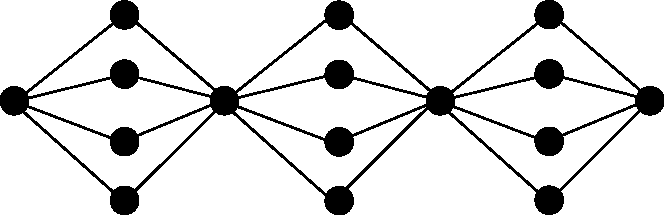
\includegraphics[scale=0.3]{fanout}
\end{center}
To avoid the spurious forking and joining, we {\it delay} the non-determinism
until and unless it is needed in {\it strict contexts} (such as the guard for an
{\tt if}, a called procedure, or a numerical primitive application).
%
Doing so collapses these forks and joins into a linear sequence of states:
\begin{center}

\includegraphics[scale=0.3]{lazy}
\end{center}

This shift does not change the concrete semantics of the language to
be lazy.  Rather, it abstracts over transitions that the original
non-deterministic semantics steps through.
%
We say the abstraction is \emph{lazy} because it delays splitting on
the values in an address until they are \emph{needed} in the
semantics. It does not change the execution order that leads to the
values that are stored in the address.

We introduce a new kind of value,
\spchoice
{$\saddr{\maddr}$}
{$\superposition{\mval{s}}$ (for ``superposition'')},
%
that represents a delayed non-deterministic choice of a value from
\spchoice
{$\msto(\maddr)$}
{$\mval{s}$}.
%
The following rules highlight the changes to the semantics:

\renewcommand{\ext}{\mathit{ext}}

\begin{align*}
\spchoice
{\force &: \Store \times \Value \to \Set(\Value) \\
 \force(\msto,\saddr{\maddr}) &= \msto(\maddr) \\
 \force(\msto,\mval) &= \setof{\mval}}
{\force &: \Value \to \Set(\Value) \\
 \force(\superposition{\mval{s}}) &= \mval{s} \\
 \force(\mval) &= \{\mval\}}
\\
%
\ev{\svar{\mvar},\menv,\mkont,\msto} &\lmachstep\;
\spchoice
{\co{\mkont,\saddr{\menv(\mvar)},\msto}}
{\co{\mkont,\superposition{\msto(\menv(\mvar))},\msto}} \\
%
\co{\kar[^\mcntr_\mlab]{\mexp,\menv,\mkaddr},\mval,\msto}
&\lmachstep\;
\ev[^{\mcntr'}]{\mexp,\menv,\msto',\kfn[^\mcntr_\mlab]{\maddr_f,\mkaddr}} \\
\text{ where }
\maddr_f &= \alloc(\mstate) \\
\msto' &=
\spchoice
{\msto \sqcup[\maddr \mapsto \force(\msto,\mval)]}
{\msto \sqcup[\maddr \mapsto \force(\mval)]} \\
%
\co{\kif[^\mcntr]{\mexpi0,\mexpi1,\menv,\mkaddr},\mval,\msto}
&\lmachstep\;
\ev[^{\mcntr'}]{\mexpi,\menv,\msto,\mkont} \\
\text{ if } \mkont &\in \msto(\mkaddr),
            \strue \in \spchoice{\force(\msto,\mval)}{\force(\mval)}
\end{align*}
Since {\tt if} guards are in strict position, we must force the value
to determine which branch to to take. The middle rule uses $\force$
only to combine with values in the store - it does not introduce
needless non-determinism.

\spchoice{
\noindent
We have two choices for how to implement lazy non-determinism.

\paragraph{Option 1: Lose precision; simplify implementation}
This semantics introduces a subtle precision difference over the
baseline. Consider a configuration where a reference to a variable and
a binding of a variable will happen in one step, since store widening
leads to stepping several states in one big ``step.'' With laziness,
the reference will mean the original binding(s) of the variable or the
new binding, because the actual store lookup is delayed one step
(i.e. laziness is administrative). Without laziness, the reference
will fan out to all the bindings of the variable before the new
binding happens and thus theoretically has an observable precision
difference. % All our benchmarks maintain their precision with lazy non-determinism, however.

\paragraph{Option 2: Regain precision; complicate implementation}
The administrative nature of laziness means that we could remove the
loss in precision by duplicating the reduction relation to specialize
variable lookup. This works since in the semantics of ISWIM with
store-allocated results consumes the value component of states in one
step. This is not the case for semantics that replicate the value
component across reductions, say for popping off exception handler
frames. Further convolution is needed to remove the administrative
nature of laziness in these semantics. Due to the increase of
conceptual and implementation complexity for negligible benefit, we
decided against this approach.

\paragraph{Our choice: option 1}
The configurations that lead to precision loss happen too rarely to
warrant the significant increase in time and memory needed for this
eager non-determinism. Indeed, were the variable reference a step
later and another binding not made in that step, the results of the
two approaches are the same. Without a widened store, lazy
non-determinism is not a complete abstraction with either approach,
but the precision gains are not immediately apparent due to fake
rebinding (a second reference to the same variable chooses a different
value from the first) and other problems. The performance and memory
gains are apparent, so we favor the simplicity over invisible
gains.}{}

\spchoice
{
\begin{theorem}[Soundness]
  If $\mstate \machstep \mstate'$ and $\mstate \sqsubseteq
  \mastate$ then there exists a $\mastate'$ such that $\mastate
  \lmachstep \mastate'$ and $\mstate' \sqsubseteq \mastate'$
\end{theorem}
Here $\sqsubseteq$ is straightforward - the LHS store must be
contained in the RHS store, and if values occur in the states, forcing
the LHS value must be a subset of forcing the corresponding RHS value.
The proof is by cases on $\mstate \machstep \mstate'$.}
{
\begin{theorem}[Completeness]For all $\mexp$,
 $\traces_{\text{Lazy}}(\mexp)$ is a complete abstraction of $\traces_{\text{ISWIM}}(\mexp)$.
\end{theorem}
We have a statement about traces because we need induction to show no
cruft values are in superposition.  The induction hypothesis tells us
that there are non-lazy traces that lead to all the values in
superposition, so when we take a lazy step, we are taking several
non-lazy steps, and we stay in sync. The other direction we just
collapse the superposition in each possibility to construct the
non-lazy traces.}

% Lazy:  cpu time: 32481 real time: 32881 gc time: 547

\subsection{Abstract compilation}

The prior optimization saved time by doing the same amount of
reasoning as before but in fewer transitions. We can exploit the same
idea---same reasoning, fewer transitions---with abstract
compilation. Abstract compilation transforms complex expressions whose
\emph{abstract} evaluation is deterministic into ``abstract
bytecodes.''  The abstract interpreter then does in one transition
what previously took many. In short, abstract compilation eliminates
unnecessary allocation, deallocation and branching. The technique is
precision preserving without store widening. We discuss the precision
differences with store widening at the end of the section.

The following example illustrates
the essence of abstract compilation effect:
\[
\mexp := \sapp{\sapp{\sapp\mvar{\mexp_1}}{\mexp_2}}{\mexp_3}
\]
makes the following transitions:
\begin{align}
& \ev[^\mcntr]{\sapp{\sapp{\sapp\mvar{\mexp_1}}{\mexp_2}}{\mexp_3},\menv,\msto_0,\mkont}\\
\machstep\; &
\ev[^{\mcntr'}]{\sapp{\sapp\mvar{\mexp_1}}{\mexp_2},\menv,\msto_1,\kar{\mexp_3,\menv,\maddr_1}}
\\
\machstep\; &
\ev[^{\mcntr''}]{\sapp\mvar{\mexp_1},\menv,\msto_2,\kar{\mexp_2,\menv,\maddr_2}}
\\
\machstep\; &
\ev[^{\mcntr'''}]{\mvar, \menv,\msto_3,\kar{\mexp_1,\menv,\maddr_3}} % {\mexp_2}
\\
\machstep\; &
\spchoice
{\co{\kar{\mexp_1,\menv,\maddr_3},\saddr{\menv(\mvar)},\msto_4}}
{\co{\kar{\mexp_1,\menv,\maddr_{f3},\maddr_{a3},\maddr_3},\superposition{\msto_4(\menv(\mvar))},\msto_4}}
\end{align}
where \(
\msto_4 = \msto_0 \sqcup [\maddr_1 \mapsto \setof{\mkont},
\maddr_2 \mapsto \setof{\kar{\compile{\mexp_3},\menv,\maddr_1}},
\maddr_3 \mapsto \setof{\kar{\compile{\mexp_2},\menv,\maddr_2}}]\).

Whereas abstract compilation gives us in one step:
\begin{align*}
\compile{\mexp}^\mcntr(\msto_0)(\menv,\epsilon,\mkont) =
\spchoice
{\co{\kar{\compile{\mexp_1},\menv,\maddr_3},\saddr{\menv(\mvar)}},\msdiff_4}
{\co{\kar{\compile{\mexp_1},\menv,\maddr_{f3},\maddr_{a3},\maddr_3},\superposition{\msto'_4(\menv(\mvar))},\msto'_4}}
\end{align*}
where
\begin{equation*}
\msdiff_4 = [\ttuple{\maddr_1}{\setof{\mkont}},
             \ttuple{\maddr_2}{\setof{\kar{\compile{\mexp_3},\menv,\maddr_1}}},
             \ttuple{\maddr_3}{\setof{\kar{\compile{\mexp_2},\menv,\maddr_2}}}]\text.
\end{equation*}

The compilation step converts expressions into functions that expect
the other components of the {\tt ev} state. Its definition in figure
\ref{fig:compile} shows close similarity to the rules for interpreting
{\tt ev} states. The next step is to change reduction rules that
create {\tt ev} states to instead call these functions. Figure
\ref{fig:caam} shows the modified reduction relation. The only change
from the previous semantics is that $\ev{}$ state construction is
replaced by calling the compiled expression. For notational coherence,
we write $\lambda^\mcntr(\mathit{args} \ldots)$ for
$\lambda(\mathit{args} \ldots, \mcntr)$ and
$\mcomp^\mcntr(\mathit{args}\ldots)$ for $\mcomp(\mathit{args}\ldots,
\mcntr)$.

\begin{figure}
\begin{align*}
\compile{\_} &: \Expr \to \Store \\
             &\phantom{: \Expr } \to \Env  \times \StoreDelta \times \Kont \times \Counter \\
             &\phantom{: \Expr } \to \State \\
\mcntr' &= \tick(\mlab,\menv,\msto,\mcntr) \\
\compile{\svar\mvar}_\msto &=
 \lambda^\mcntr(\menv,\msdiff,\mkont) .
\spchoice
{\co{\mkont,\saddr{\menv(\mvar)}},\msdiff}
{\co{\mkont,\superposition{\msto(\menv(\mvar))}},\msdiff}
\\
\compile{\slit\mlit}_\msto &= \lambda^\mcntr(\menv,\msdiff,\mkont) .
\co{\mkont,\mlit},\msdiff
\\
\compile{\slam\mvar\mexp}_\msto &= \lambda^\mcntr(\menv,\msdiff,\mkont) .
\co{\mkont,\clos{\mvar,\compile{\mexp},\menv}},\msdiff
\\
\compile{\sapp[^\mlab]{\mexpi0}{\mexpi1}}_\msto &= \lambda^\mcntr(\menv,\msdiff,\mkont) .
\compile{\mexpi0}^{\mcntr'}(\menv,\msdiff',\kar[_\mlab^\mcntr]{\compile{\mexpi1},\menv,\mkaddr})
\\
&\setlength\arraycolsep{5pt}
\begin{array}{lrl}
\text{ where } & \mkaddr = \allockont^\mcntr_\mlab(\msto,\mkont) \\
               & \msdiff' = \cons{\ttuple{\mkaddr}{\setof{\mkont}}}{\msdiff}
\end{array}
\\
\compile{\sif[^\mlab]{\mexpi0}{\mexpi1}{\mexpi2}}_\msto &= \lambda^\mcntr(\menv,\msdiff,\mkont) .
\compile{\mexpi0}^{\mcntr'}(\menv,\msdiff',\kif[^\mcntr]{\compile{\mexpi1},\compile{\mexpi2},\menv,\maddr})
\\
&\text{ where }\mkaddr = \allockont^\mcntr_\mlab(\msto,\mkont) \\
&\phantom{\text{ where }} \msdiff' = \cons{\ttuple{\mkaddr}{\setof{\mkont}}}{\msdiff}
\end{align*}
\caption{Abstract compilation}
\label{fig:compile}
\end{figure}

\begin{figure}
\begin{gather*}
\begin{align*}
\traces(\mexp) &= \setof{ \inject(\compile{\mexp}^\mtcntr_\bot(\bot,\epsilon,\kmt)) \multimachstep \mstate}
                    \text{ where } \\
\inject(\mastate,\msdiff) &= \wn(\mastate,\replay(\msdiff,\bot)) \\
\wn(\mastate,\msto) \machstep \wn(\mastate',\msto') &\iff \mastate \cmachstep_\msto \mastate',\msdiff \\
\msdiff \text{ is such that } &\replay(\msdiff,\msto) = \msto'
\end{align*}
\\[2mm]
\begin{align*}
%% CONTINUE
\co{\kmt,\mval} &\cmachstep_\msto
\ans{\mval'},\epsilon \text{ if } \mval' \in \spchoice{\force(\msto,\mval)}{\force(\mval)}
\\
\co{\kar[^\mcntr_\mlab]{\mcomp,\menv,\mkaddr},\mval} & \cmachstep_\msto
\mcomp^\mcntr(\msto)(\menv,\msdiff,\kfn[^\mcntr_\mlab]{\maddr_f,\mkaddr}) \\
\text{ where } \maddr_f &= \alloc(\mstate) \\
               \msdiff &= \cons{\ttuple{\maddr_f}{\force(\msto,\mval)}}{\epsilon}
\\
\co{\kfn[^\mcntr_\mlab]{\maddr_f,\mkaddr},\mval} & \cmachstep_\msto
\ap[^\mcntr_\mlab]{\mval,\mval\mkont},\epsilon \\
\text{ if }\mval &\in \msto(\maddr_f), \mkont \in \msto(\mkaddr)
\\
\co{\kif[^\mcntr]{\mcompi0,\mcompi1,\menv,\maddr},\strue} & \cmachstep_\msto
\mcompi{0}^\mcntr(\msto)(\menv,\epsilon,\mkont)
\text{ if }\mkont\in\msto(\maddr)
\\
\co{\kif[^\mcntr]{\mcompi0,\mcompi1,\menv,\maddr},\sfalse} & \cmachstep_\msto
\mcompi{1}^\mcntr(\msto)(\menv,\epsilon,\mkont)
\text{ if }\mkont\in\msto(\maddr)
\\[2mm]
%% APPLY
\ap[^\mcntr_\mlab]{\clos{\mvar,\mcomp,\menv},\mval,\mkont} & \cmachstep_\msto
\mcomp^{\mcntr'}(\msto)(\menv',\msdiff,\mkont) \\
\text{ where }\menv' &= \menv[\mvar\mapsto\maddr] \\
              \msdiff &= \cons{\ttuple{\maddr}{\force(\msto,\mval)}}{\epsilon}
\\
\ap{\mop,\mval,\mkont} & \cmachstep_\msto
\co{\mkont,\mval'},\epsilon \\
\text{ where } \mvalx{u} &\in \spchoice{\force(\msto,\mval)}{\force(\mval)}, \mval'\in\interpdelta(\mop,\mvalx{u})
\end{align*}
\end{gather*}
\caption{Abstract abstract machine for compiled ISWIM}
\label{fig:caam}
\end{figure}

\paragraph{Correctness}
The correctness of abstract compilation seems obvious, but it has
never before been rigorously proved. What constitutes correctness in
the case of dropped states, anyway? Applying an abstract bytecode's
function does many ``steps'' in one go, at the end of which, the two
semantics line up again (modulo representation of expressions). This
constitutes the use of a notion of stuttering. We provide a formal
analysis of abstract compilation \emph{without} store widening with a proof
of a stuttering bisimulation~\cite{ianjohnson:BCG88} between this
semantics and lazy non-determinism without widening to show precision
preservation. %We revisit store widening at the end of the section.

The number of transitions that can occur in succession from an
abstract bytecode is roughly bounded by the amount of expression
nesting in the program. The partial order that defines subexpressions
smaller than the expression in which they occur is well-founded, so we
use this observation to drive our use of a well-founded equivalence
bisimulation (WEB)~\cite{ianjohnson:manolios-diss}. WEBs are equivalent to the notion of a stuttering
bisimulation, but are more amenable to mechanisation (and thus
rigorous proof). They also only require reasoning over one step of the
reduction relation, which makes the proof concise.

We define a refinement from non-compiled to compiled states by
``committing'' all the actions of an $\ev{}$ state (defined similarly to
$\compile{\_}$, but immediately applies the functions), and
subsequently changing all expressions with their compiled
variants. Since WEBs are for single transition systems, a WEB
refinement is over the disjoint union of our two semantics, and the
equivalence relation we use is just that a state is related to its
refined state (and itself). Call this relation $B$.

Before we prove this setup is indeed a WEB, we need one lemma that
applying an abstract bytecode's function is equal to refining the
corresponding $\ev{}$ state:
%
\begin{lemma}[Compile/commit]
Let $\mastate,\msdiff' = \compile{\mexp}^\mcntr_{r(\msto)}(\menv,\msdiff,r(\mkont))$.
Let $\wn(\mastate',\msto') = r(\ev[^\mcntr]{\mexp,\menv,\msto,\mkont})$.
$\wn(\mastate,\replay(\msdiff',\msto)) = \wn(\mastate',\replay(\msdiff,\msto'))$.
\end{lemma}
The proof is by induction on $\mexp$.

\begin{theorem}[Precision preservation]
$B$ is a WEB on $\lmachstep \uplus \machstep$
\end{theorem}

The proof follows by cases on $\lmachstep \uplus \machstep$ with the
WEB \emph{witness} being the well-order on expressions (with a $\bot$
element), and the following $\erankt$, $\erankl$ functions:

\begin{align*}
\erankt(\ev[^\mcntr]{\mexp,\menv,\msto,\mkont}) &= \mexp \\
\erankt(\mstate) &= \bot \quad \text{otherwise} \\
\erankl(s,s') &= 0
\end{align*}
All cases are either simple steps or appeals to the well-order on $\erankt$'s range. The other rank function,
$\erankl$ is unnecessary, so we just make it the constant 0
function. The $\cmachstep$ cases are trivial.

\paragraph{Wide store and abstract compilation}
The fact that many changes happen in one step also makes the
comparison with the widened lazy semantics more subtle. It is possible
for different stores to occur between the different semantics because
abstract compilation can change the order in which the store is
changed. Consider the case where before we might call the same
function from two different places in 3 and 2 steps respectively,
compilation can make that 2 and 1, reversing the order that we bind
values in the store, leading to a mismatch from the previous
semantics. This kind of cross-step store poisoning is inevitable when
a store is shared between several traces. The binding could have just
as easily been observed the other way around in the non-compiled
semantics. Call $\camachstep$ the result of the widening operator from
the previous section on $\cmachstep$.

% Compile: cpu time: 255397 real time: 261532 gc time: 2947

% \noindent
% Compile + Lazy: cpu time: 31173 real time: 31642 gc time: 739

%\newpage

%% Delta Store +k Compile + Lazy:
%%    cpu time: 668 real time: 686 gc time: 41

\subsection{Imperative, preallocated data structures}

Thus far, we have made our optimizations in a purely functional
manner. For the final push for performance, we need to dip into the
imperative. In this section, we show an alternative representation of
the store and seen set that are more space-efficient and are amenable
to destructive updates.

The following transfer function has several components that can be
destructively updated, and intermediate sets can be elided by adding
to global sets. In fact, the log of store deltas can be removed as
well, by updating the store in-place, and on lookup, using the first
value timestamped $\le$ the current timestamp. We start with the
purely functional view.

\subsubsection{Pure setup for imperative implementation}

The store maps to a stack of timestamped sets of abstract values.

\begin{align*}
\msto \in \Store &= \Addr \to \Valstack \\
\mvalstack \in \Valstack &= (\Timestamp \times \wp(\Storeable))^*
\end{align*}

Here we formally define what lookup and update mean at a given
timestamp.

\begin{align*}
\lookup(\mvalstack,t) &=
  \left\{
    \begin{array}{ll}
      \mval{s} & \text{ if } \mvalstack = \cons{\ttuple{t'}{\mval{s}}}{\mvalstack'}, t' \le t \\
      \mval{s'} & \text{ if } \mvalstack = \cons{\ttuple{t'}{\mval{s}}}{\cons{\ttuple{t''}{\mval{s'}}}{\mvalstack'}}, t' > t
    \end{array}\right. \\
\msto \sqcup_t [\maddr \mapsto \mval{s}] &= \msto[\maddr \mapsto \mvalstack],\changep \\
 (\mvalstack,\changep) &= \msto(\maddr)\sqcup_t \mval{s} \\
\epsilon \sqcup_t \mval{s} &= \ttuple{t}{\mval{s}} \\
\cons{\ttuple{t'}{\mval{s}}}{\mvalstack} \sqcup_t \mval{s'} &= \cons{\ttuple{t'}{\mval{s}\sqcup\mval{s'}}}{\mvalstack},\strue \text{ if } t' > t \\
\mvalstack \sqcup_t \mval{s} &= \cons{\ttuple{t+1}{\mval{s^*}}}{\mvalstack},\strue
           \text{ if } \mval{s'} \neq \mval{s^*} \\
 \mval{s'} &= \lookup(\msto(\maddr),t) \\
 \mval{s^*} &= \mval{s} \sqcup \mval{s'} \\
\mvalstack \sqcup_t \mval{s} &= \mvalstack,\sfalse \text{ otherwise}
\end{align*}

For the purposes of space, we reuse the $\cmachstep$ semantics,
although the $\replay$ of the produced $\msdiff$ objects should be
in-place, and the $\lookup$ function should be using this
single-threaded store.  Because the store has all the temporal
information baked into it, we rephrase the core semantics in terms of
a transfer function. The least fixed-point of this function gives a
more compact representation of the reduction relation of the previous
section.

\begin{align*}
\System &= (\widehat{\State} \to {\Timestamp}^*) \times \wp(\widehat{\State}) \times \Store \times \Timestamp \\
{\mathcal F} &: \System \to \System \\
{\mathcal F}(S,F, \msto,t) &= (S',F',\msto', t') \\
\text{ where }
I &= \setof{(\mastate',\msdiff) \mid
       \mastate \in F,
       \mastate \cmachstep_{\msto^*} \mastate',\msdiff} \\
\msto^* &= \lambda \maddr.\lookup(\msto(\maddr),t) \\
\ttuple{\msto'}{\changep} &= \replay(\appendall(\setof{\msdiff \mid (\_,\msdiff) \in I}),\msto) \\
t' &= \left\{\begin{array}{ll} t+1 & \text{ if } \changep \\
              t   & \text{ otherwise}
             \end{array}\right. \\
F' &= \setof{\mastate \mid (\mastate,\_) \in I, \changep \vee S(\mastate) \neq \cons{t}{\_}} \\
S' &= \lambda \mastate. \left\{\begin{array}{ll}
                               \cons{t'}{S(\mastate)} & \text{ if } \mastate \in F' \\
                               S(\mastate) & \text{ otherwise}
                             \end{array}\right.
\end{align*}

We prove semantic equivalence with the previous semantics with a
lock-step bisimulation with the stack of stores abstraction, which
follow from equational reasoning from the following lemmas:

\begin{lemma}
Stores of value stacks completely abstract stacks of stores.
\end{lemma}
This depends on some wellformedness conditions about the order of the
stacks. The store of value stacks can be translated to a stack of
stores by taking successive ``snapshots'' of the store at different
timestamps from the max timestamp it holds down to 0. Vice versa, we
replay the changes across adjacent stores in the stack.

We apply a similar construction to the different representation of seen states in order to get the final result:

\begin{theorem}
${\mathcal F}$ is a complete abstraction of $\camachstep$.
\end{theorem}

\subsubsection{Pure to imperative}

The intermediate data structures of the above transfer function can all be streamlined into globals that are destructively updated. In particular, there are 5 globals:

\begin{enumerate}
\item{$S$: the \emph{seen} set, though made a map for faster membership tests and updates.}
\item{$F$: the \emph{frontier} set, which must be persisent or copied for the iteration through the set to be correct.}
\item{$\msto$: the store, which represents all stores that occur in the machine semantics.}
\item{$t$: the timestamp, or length of the store chain - all stores that occur in the semantics are totally ordered due to single-threading the store.}
\item{$\changep$: whether there has been a store change stepping all states in $F$.}
\end{enumerate}

The reduction relation would then instead of building store deltas,
update the global store. We would also not view it as a general
relation, but a function that adds all next states to $F$ if they have
not already been seen. At the end of iterating through $F$, $S$ is
updated with the new states at the next timestamp.

\subsubsection{Pre-allocating the store}

Internally, the algorithm at this stage uses hash tables to model the store.
%
This is because stores used to be distributed to all states, which
required a compact, dynamic representation.
%
But, such a dynamic structure isn't necessary when we know the
structure of the store in advance: we know all possible entries, and
we know its maximum size.

In a monovariant analysis, the domain of the store is
exactly the set of expressions in the program.
%
If we label each expression with a unique natural, the analysis can
index directly into the store without a hash or a collision.
%
Even for polyvariant analyses, it is possible to compute the maximum
number of addresses and similarly pre-allocate either the spine of the
store or (if memory is no concern) the entire store.

\section{Evaluation}
\label{sec:eval}

We have implemented, optimized, and evaluated an analysis framework
supporting higher-order functions, state, first-class control,
compound data, and a large number of primitive kinds of data and
operations such as floating point, complex, and exact rational
arithmetic.  The analysis is evaluated against a suite of Scheme benchmarks
drawn from the literature.
%
For each benchmark, we collect analysis times, peak memory usage, and
the rate of states-per-second explored by the analysis for each of the
optimizations discussed in section~\ref{sec:opt}, cumulatively
applied.  The analysis is stopped after consuming 30 minutes of time
or 1 gigabyte of space.  When presenting \emph{relative} numbers, we
use the timeout limits as a lower bound on the actual time required,
thus giving a conservative estimate of improvements.

All benchmarks are calculated as an average of 5 runs, done in
parallel, on an 12-core, 64-bit Intel Xeon machine running at 2.40GHz
with 12Gb of memory.

Many benchmarks cause the baseline analyzer to take longer than 30
minutes or to consume more 1 gigabyte of memory, at which point the
analysis is stopped.  This is the case for the largest benchmark
program, {\bf nucleic}, which is 3,500 lines of code and takes under a minute in the
most optimized analyzer.  For those benchmarks that did complete on
the baseline, the optimized analyzer outperformed the baseline by a
factor of two to three orders of magnitude.
% safer to not give exact factors
% 475 to 4,382.

We use the following set of benchmarks:
\begin{figure}
\centering
\include{bench-overview}
\caption{Overview performance comparison between baseline and
  optimized analyzer (entries of \text{{\small $t$}} mean timeout, and \text{{\small $m$}} mean out of memory).}
\label{fig:bench-overview}
\end{figure}

\begin{enumerate}  %% Maybe use ``dictionary'' style enumeration.

\item {\bf nucleic}: a floating-point intensive application taken from
  molecular biology that has been used widely in benchmarking
  functional language
  implementations~\cite{dvanhorn:Hartel1996Benchmarking} and analyses
  (e.g.~\cite{dvanhorn:wright-jagannathan-toplas98,dvanhorn:jagannathan-etal-popl98}).
  It is a constraint satisfaction algorithm used to determine the
  three-dimensional structure of nucleic acids.

\item {\bf matrix} tests whether a matrix is maximal among all
  matrices of the same dimension obtainable by simple reordering of
  rows and columns and negation of any subset of rows and columns.  It
  is written in continuation-passing style (used in
  \cite{dvanhorn:wright-jagannathan-toplas98,dvanhorn:jagannathan-etal-popl98}).


\item {\bf nbody}: implementation~\cite{ianjohnson:nbody87} of the
  Greengard multipole algorithm for computing gravitational forces on
  point masses distributed uniformly in a cube (used in
  \cite{dvanhorn:wright-jagannathan-toplas98,dvanhorn:jagannathan-etal-popl98}).

\item {\bf earley}: Earley's parsing algorithm, applied to a 15-symbol
  input according to a simple ambiguous grammar.  A real program,
  applied to small data whose exponential behavior leads to a peak
  heap size of half a gigabyte or more during concrete execution.

\item {\bf maze}: generates a random maze using Scheme's {\tt
  call/cc} operation and finds a path solving
  the maze (used in
  \cite{dvanhorn:wright-jagannathan-toplas98,dvanhorn:jagannathan-etal-popl98}).

\item {\bf church}: tests distributivity of multiplication over
  addition for Church numerals (introduced by
  \cite{dvanhorn:Vardoulakis2011CFA2}).

\item {\bf lattice}: enumerates the order-preserving maps between two
  finite lattices (used in
  \cite{dvanhorn:wright-jagannathan-toplas98,dvanhorn:jagannathan-etal-popl98}).

\item {\bf boyer}: a term-rewriting theorem prover (used in
  \cite{dvanhorn:wright-jagannathan-toplas98,dvanhorn:jagannathan-etal-popl98}).

\item {\bf mbrotZ}: generates Mandelbrot set fractal using complex
  numbers.

\item {\bf graphs}: counts the number of directed graphs with a
  distinguished root and \(k\) vertices, each having out-degree at
  most 2. It is written in a continuation-passing style and makes
  extensive use of higher-order procedures---it creates closures
  almost as often as it performs non-tail procedure calls (used by
  \cite{dvanhorn:wright-jagannathan-toplas98,dvanhorn:jagannathan-etal-popl98}).
\end{enumerate}

%% 400 lines for the core, 700 lines for
%% abstraction over optimizations, 1500 lines for primitives and standard
%% list operations, 700 lines for instantiations to different
%% optimizations and 300 for parsing and macro transformers.

Figure~\ref{fig:bench-overview} gives an overview of the benchmark
results in terms of absolute time, space, and speed between the
baseline and most optimized analyzer.  Figure~\ref{fig:bench-all}
plots the factors of improvement over the baseline for each
optimization step. The dip we see in transition rate even though time
taken decreases is to be expected - fewer ``easy'' states are added by
abstract compilation. It increases again with the introduced
algorithmic improvements. Accumulating store changes in addition to
maintaining the store accounts for the higher memory usage when using
the store delta technique without further improvements.

\begin{figure*}
\begin{center}
  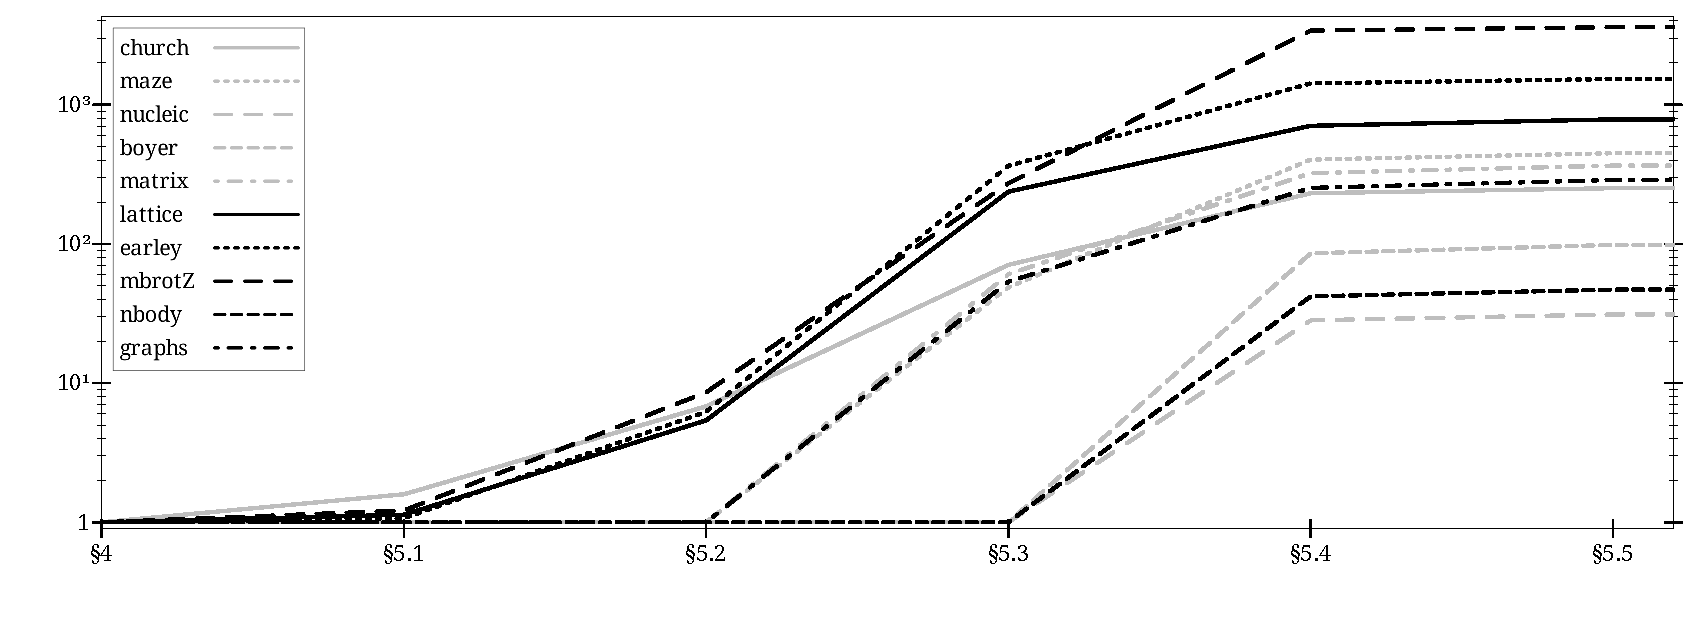
\includegraphics[width=6.5in]{all-relative-time}

  (a) Total analysis time

  \vspace{1em}
  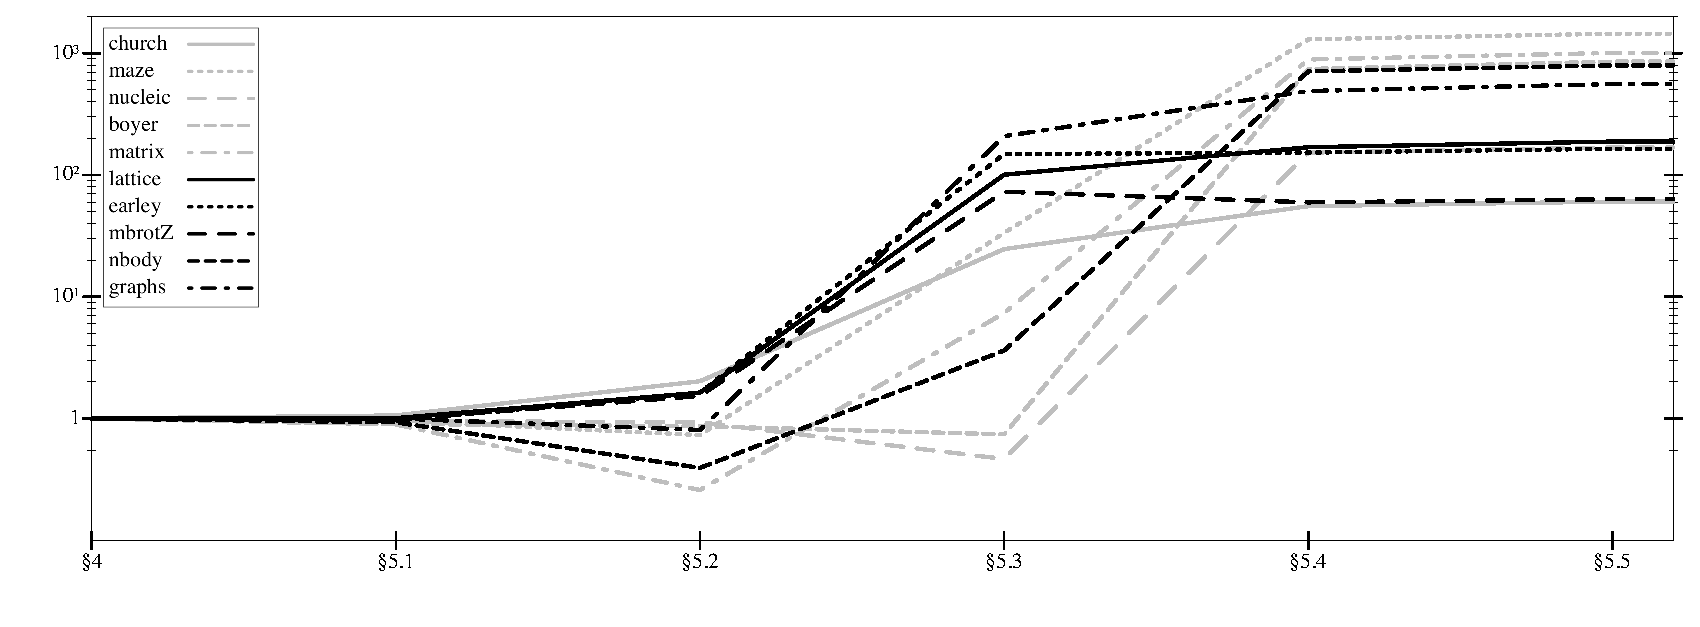
\includegraphics[width=6.5in]{all-relative-speed}

  (b) Rate of state transitions

  \vspace{1em}
  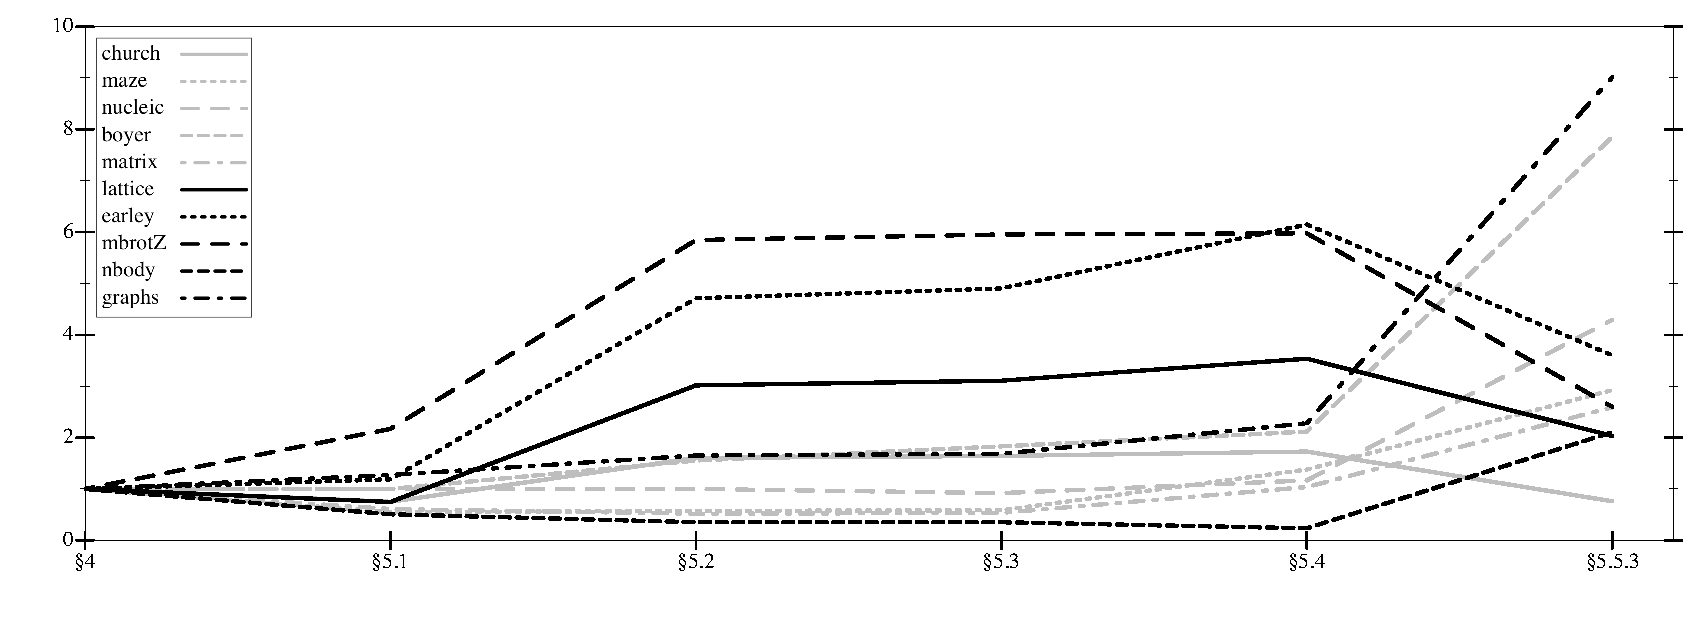
\includegraphics[width=6.5in]{all-relative-space}

  (c) Peak memory usage
\end{center}
\caption{Factors of improvement over baseline for each step of
  optimization (bigger is better).}
\label{fig:bench-all}
\end{figure*}

We evaluated the precision of these techniques with a singleton
variable analysis to find opportunities to inline constants and closed
functions. We found no change in the results across all
implementations, including Shivers' timestamp approximation.

Source code of the implementation and benchmark suite is at:

\begin{center}
\url{https://github.com/dvanhorn/oaam}
\end{center}

\paragraph{Comparison with other flow analysis implementations}

The analysis considered here computes results similar to Earl, et al.'s
0-CFA implementation~\cite{dvanhorn:Earl2012Introspective}, which
times out on the \Church{} benchmark because it does not widen the
store as described for our baseline evaluator.  So even though it
offers a fair point of comparison, a more thorough evaluation is
probably uninformative as the other benchmarks are likely to timeout
as well (and it would require significant effort to extend their
implementation with the features needed to analyze our benchmark
suite).  That implementation is evaluated against much smaller
benchmarks: the largest program is 30 lines.

Vardoulakis and Shivers evaluate their CFA2
analyzer~\cite{dvanhorn:Vardoulakis2011CFA2} against a variant of
0-CFA defined in their framework and the example we draw on is the
largest benchmark Vardoulakis and Shivers consider.  More work would
be required to scale the analyzer to the set of features required by
our benchmarks.

The only analyzers we were able to find that proved capable of
analyzing the full suite of benchmarks considered here were the Soft
Typing system of Wright and
Cartwright~\cite{dvanhorn:Wright1997Practical} and, in many ways its
successor, the Polymorphic splitting system of Wright and
Jagannathan~\cite{dvanhorn:wright-jagannathan-toplas98}.\footnote{This
  is not a coincidence; these papers set a high standard for
  evaluation, which we consciously aimed to approach.}  Unfortunately,
these analyses compute an inherently different and incomparable form
of analysis.  Consequently, we have omitted a complete comparison with
these implementations.  The AAM approach provides more precision in
terms of temporal-ordering of program states, which comes at a cost
that can be avoided in constraint-based approaches.  Consequently
implementation techniques cannot be ``ported'' between these two
approaches.  However, our optimized implementation is within an order
of magnitude of the performance of Wright and Jaganathan's analyzer.
Although we would like to improve this to be more competitive, the
optimized AAM approach still has many strengths to recommend it in
terms of precision, ease of implementation and verification, and rapid
design. We can get closer to their performance by relying on the
representation of addresses and the behavior of $\alloc$ to
pre-allocate most data structures and split the abstract store out
into parts that are more quickly accessed and updated. The first two
of our optimizations can still be applied to an analysis that does
abstract garbage collection~\cite{dvanhorn:Might:2006:GammaCFA},
whereas the polymorphic splitting implementation is tied strongly to a
single-threaded store.

\section{Related work}
\label{sec:related}

\paragraph{Abstracting Abstract Machines}

This work clearly closely follows Van Horn and Might's original papers
on abstracting abstract
machines~\cite{dvanhorn:VanHorn2011Abstracting,dvanhorn:VanHorn2012Systematic},
which in turn is one piece of the large body of research on flow
analysis for higher-order languages (see
Midtgaard~\cite{dvanhorn:Midtgaard2011Controlflow} for a thorough
survey).  The AAM approach sits at the confluence of two major lines
of research: (1) the study of abstract
machines~\cite{dvanhorn:landin-64} and their systematic
construction~\cite{dvanhorn:reynolds-hosc98}, and (2) the theory of
abstract interpretation
\cite{dvanhorn:Cousot:1977:AI,dvanhorn:Cousot1979Systematic}.


\paragraph{Frameworks for flow analysis of higher-order programs}

Besides the original AAM work, the analysis most similar to that
presented in section~\ref{sec:aam} is the infinitary control-flow
analysis of Nielson and Nielson~\cite{dvanhorn:nielson-nielson-popl97}
and the unified treatment of flow analysis by Jagannathan and
Weeks~\cite{dvanhorn:jagannathan-weeks-popl95}.  Both are
parameterized in such a way that in the limit, the analysis is
equivalent to an interpreter for the language, just as is the case
here.  What is different is that both give a constraint-based
formulation of the abstract semantics rather than a finite machine
model.

\paragraph{Abstract compilation}

Boucher and Feeley \cite{dvanhorn:Boucher1996Abstract} introduced the
idea of abstract compilation, which used closure generation
\cite{dvanhorn:Feeley1987Using} to improve the performance of control
flow analysis.  We have adapted the closure generation technique from
compositional evaluators to abstract machines and applied it to similar
effect.

\paragraph{Constraint-based program analysis for higher-order languages}

Constraint-based program analyses
(e.g.~\cite{dvanhorn:nielson-nielson-popl97,dvanhorn:wright-jagannathan-toplas98,dvanhorn:Meunier2006Modular,dvanhorn:steckler-wand-toplas97})
typically compute sets of abstract values for each program point.
These values approximate values arising at run-time for each
program point.  Value sets are computed as the least solution to a set
of (inclusion or equality) constraints.  The
constraints must be designed and proved as a sound approximation of
the semantics.  Efficient implementations of these kinds of analyses
often take the form of worklist-based graph algorithms for constraint
solving, and are thus quite different from the interpreter
implementation.  The approach thus requires effort in constraint
system design and implementation, and the resulting system require
verification effort to prove the constraint system is sound and that
the implementation is correct.

This effort increases substantially as the complexity of the analyzed
language increases.  Both the work of maintaining the concrete
semantics and constraint system (and the relations between them) must
be scaled simultaneously.  However, constraint systems, which have
been extensively studied in their own right, enjoy efficient
implementation techniques and can be expressed in declarative logic
languages that are heavily
optimized~\cite{dvanhorn:bravenboer-smaragdakis-oopsla09}.
Consequently, constraint-based analyses can be computed quickly.  For
example, Jagannathan and Wright's polymorphic splitting
implementation~\cite{dvanhorn:wright-jagannathan-toplas98} analyses
the \Church{} benchmark about 25 times faster than the fastest
implementation considered here.  These analyses compute very different
things, so the performance comparison is not apples-to-apples.

The AAM approach, and the state transition graphs it generates, encodes
temporal properties not found in classical constraint-based analyses
for higher-order programs.
%
Such analyses (ultimately) compute judgments on program terms and
contexts, e.g., at expression $e$, variable $x$ may have value $v$.
%
The judgments do not relate the order in which expressions and context
may be evaluated in a program, e.g., it has nothing
to say with regard to question like, ``Do we always evaluate $e_1$
before $e_2$?'' or ``Is it always the case that a file handle is
opened, read and then closed in that order?''
%
The state transition graphs can answer these kinds of queries, but
this does not come for free: respecting temporal order imposes an
order in which states and terms may be evaluated \emph{during} the
analysis.

\section{Conclusion}
\label{sec:conclusion}

Abstract machines are not only a good model for rapid analysis
development, they can be systematically developed into efficient
algorithms that can be proved correct. We view the primary
contribution of this work as a systematic path that eases the design,
verification, and implementation of analyses using the abstracting
abstract machine approach to within a factor of performant
constraint-based analyses.

%% \acks Sam Tobin-Hochstadt for encouragement and feedback -- he was
%% the first to prompt us to look into how make effective
%% implementations of the AAM approach.

%% Vincent St Amour and Mitchell Wand for feedback on early drafts.
%% Greg Morrisset and Matthias Felleisen for discussions.

%% NSF, DARPA


\paragraph{Acknowledgments}

We thank Suresh Jagannathan for providing source code to the
polymorphic splitting
analyzer~\cite{dvanhorn:wright-jagannathan-toplas98} and Ilya Sergey
for the introspective pushdown
analyzer~\cite{dvanhorn:Earl2012Introspective}.


\balance
\bibliographystyle{plain}
%\input{paper.bbl}
\bibliography{local,bibliography}

% \include{appendix}

\end{document}

\bibliography{local,bibliography}

% \appendix
\section{Relation to Uniform \(k\)-CFA (A Case Against Acceptability)}
\label{sec:accept}

\cite{dvanhorn:nielson-nielson-popl97} \cite{dvanhorn:Neilson:1999}

This machine's allocation strategy mimics the Uniform k-CFA analysis
in Principles of Program Analysis, which is defined in terms of
``$\delta$ contours.''  However, because the machine represetation makes
context explicit via continuations, we can calculate these contours
rather than thread them throught the evaluator.  In other words, we
can use the CESK* machine without modification to obtain Uniform k-CFA
by way of a simple allocation strategy.  (In this way, it's a
simplification of the presentation in JFP.)

NNH uses a coinductive acceptability relation to specify Uniform
k-CFA:

\[
   C,R \models^{ce}_\delta E
\]

The cache and global environment form a finite store-like structure
holding bindings and return values.  The contour environment ce maps
variables to locations in R which contains their bindings, just as the
environment of the CESK* machine does.  The current contour delta is a
string of application labels describing the enclosing context under
which this term is being analyzed (or evaluated).  If you view the
acceptability relation as a big-step evalator, the
$(\widehat C,\widehat\rho)$ component should be seen as a global
store ce is the environment mapping variables to their locations.

Starting form the initial configuration for a program and iterating
the machine transition relation until reaching a fixpoint of reachable
states will \emph{underestimate} the acceptability relation of Uniform
k-CFA.  You can recover acceptability by feeding this store back into
the initial configuration and iterating again.  Repeating this process
until a complete run of the program reaches no new states will be the
least solution that is acceptable.

HOWEVER.  Why should we care about acceptability?  What this
machine computes is safe.  In other words, it computes a more
precise characterization of the run-time behavior of a program.  In
doing is so, it actually saves work (as can be seen above).

An Example:

\begin{alltt}
 (let ((id (\(\lambda\) (x) x)))
   (begin (id 1) (id 2)))
\end{alltt}

Under Uniform 0-CFA, we would have:
\[
   [{\tt x} \mapsto \{{\tt 1}, {\tt 2}\}] \in \widehat\rho
\]

in the least solution to $\models$.  This says that, when run, 'x' is
bound to 1 or 2.

Under the machine semantics using a 0CFA allocation policy, the trace
semantics of the machine show that x is bound to 1, and that at some
later point, x becomes bound to 1 or 2.  Moreover, the machine would
show that (id 1) evaluates to 1 and only 1, while Uniform 0CFA must
give that (id 1) is either 1 or 2 to be acceptable.  We don't see any
value in these kinds of false flows that are due to the global and
timeless aspects of C,R which acceptability requires the heap to be
both finite and unchanging over the course of abstract
interpretation. (Another view of the difference: the machine abstracts
a program's execution as a \emph{finite state machine} that mimics the
machine interpretation of the program; the aceptability relation of
Uniform \(k\)-CFA abstracts a program's execution as a \emph{finite
  map} that mimics the big-step evaluator: from terms to (sets of)
values.)


\subsection{Another problem with acceptability: Temporal ignorance}

The small-step approach to static analysis brings subtle yet important temporal
richness not found in classical analyses for higher-order programs.
%
Classical analyses (ultimately) compute judgments on program terms and
contexts, e.g., at expression $e$, value $x$ may have value $v$.
%
The judgments do not relate the order in which expressions and context may be
evaluated in a program, e.g., a classical analysis has nothing to say with
regard to question like, ``Do we always evaluate $e_1$ before $e_2$?'' or ``Is
it always the case that a file handle is opened, read and then closed in that
order?''

Small-step analyses, by their nature, encode the temporal relationships between
abstract states.
%
It is sensible to make temporal queries of a small-step analysis.
%
Of course, this does not come for free: respecting temporal order imposes an
order in which states and terms may be evaluated \emph{during} the analysis.
%
Classical analyses can (and do) evaluate expressions in any order, or in some
cases, even in parallel~\cite{might:Prabhu:2010:EigenCFA}.
%
Relaxing that restriction on order affords additional optimizations that we
have \emph{not} performed.

We avoid sacrificing order not simply because we are interested in the
questions it allows us to ask, but because considering temporal order actually
improves the precision of the analysis itself.



\section{Pushdown Analysis}

It is straightforward to instantiate a \emph{pushdown} abstraction by
bounding only the variable binding portion of the heap, but using a
unique allocation strategy for continuations.  Such a strategy
abstracts a program's execution as a \emph{pushdown automata}
that mimics the machine interpretation.  This strategy therefore
models the abstract stack in a true stack like fashion and always
properly matches function calls with their return.

Although such analyses can be formulated straightforwardly in the
abstract machine approach, it is not clear all of the techniques of
this paper can be applied to similar effect in the pushdown context.
The main problem is calculation of an analysis can no longer be
computed as the fixed point of the machine transition relation.
Although there are several implementations (CFA2,ICFP'12), they
operate at speeds roughly on par with our starting point: unoptimized
store widened
machines. \cite{dvanhorn:Earl2012Introspective,dvanhorn:Vardoulakis2011CFA2}

\section{Proof: laziness is precision-preserving}
Given widened machine configurations, we can show that lazy
non-determinism is precision-preserving in the cases that application
positions are store-allocated and not. We first show the latter since
it uses less cluttered transition rules. The high level is that the
``fan-out'' of non-determinism is collapsed back in the store (in the
store-allocated applications case) or delayed a single step by
laziness that would have happened in a step of strictness.

Details of lazy machine given as a diff from the strict machine. \\
State space of $lazy-\widehat{CESK}^*_t$ varies just in
$\mathit{Value}$ (storable values do not change):
\begin{align*}
\mval \in \mathit{Value} &::= z \mid b \mid o \mid \saddr{\maddr} \\
\end{align*}

We define a relation between strict and lazy machines that illustrates
the quotient that the lazy states embody.

\newcommand{\vapprx}[3]{#1 \cong_{#2} #3}
\newcommand{\kapprx}[3]{#1 \cong_{#2} #3}
\newcommand{\lapprx}[3]{#1 \approx_{#2} #3}
\newcommand{\apprx}[3]{#1 \sim_{#2} #3}
\newcommand{\capprx}[2]{#1 \sim #2}

\begin{mathpar}
\inferrule{\mval' \in force(\msto, \mval)}
          {\vapprx{\mval}{\msto}{\mval'}} \quad
\inferrule{\ans{\mval} \in cs}{\lapprx{\ans{\mval}}{\msto}{cs}} \quad
\inferrule{\ev{\mexp, \menv, \mkont, \mcntr} \in cs}
          {\lapprx{\ev{\mexp, \menv,\mkont, \mcntr}}{\msto}{cs}} \\
\inferrule{\co{\mkont, \mval'} \in cs \\
           \vapprx{\mval}{\msto}{\mval'}}
          {\lapprx{\co{\mkont, \mval}}{\msto}{cs}} \quad
\inferrule{\ap{\mval_0, \mval_1, \mkont} \in cs \\
           \vapprx{\mval_1}{\msto}{\mval_1'}}
          {\lapprx{\ap{\mval_0, \mval_1', \mkont}}{\msto}{cs}} \\
\inferrule{\ev{\mexp, \menv, \mkont} \in lcs}
          {\apprx{\ev{\mexp, \menv,\mkont}}{\msto}{lcs}} \quad
\inferrule{\ans{\mval} \in lcs \\
           \vapprx{\mval}{\msto}{\mval'}}
          {\apprx{\ans{\mval'}}{\msto}{lcs}} \\
\inferrule{\co{\mkont, \mval} \in lcs \\
           \vapprx{\mval}{\msto}{\mval'}}
          {\apprx{\co{\mkont, \mval'}}{\msto}{lcs}} \quad
\inferrule{\ap{\mval_0, \mval_1, \mkont} \in lcs \\
           \vapprx{\mval_1}{\msto}{\mval_1'}}
          {\apprx{\ap{\mval_0, \mval_1', \mkont}}{\msto}{lcs}} \\
\inferrule{\forall lc \in lcs, \lapprx{lc}{\msto}{cs} \\
           \forall c \in cs, \apprx{c}{\msto}{lcs}}
          {\capprx{(lcs, \msto)}{(cs, \msto)}}
\end{mathpar}

We also need metafunctions for adding and removing a store component
from states. These are straightforwardly defined, so just name them
$wn$ and $nw$ respectively.
%% c2vc(<e^l r k d>,s) = <e^l r s k d>
%% c2vc(<v k d>,s) = <v s k d>
%% vc2c(<e^l r s k d>) = <e^l r k d>
%% vc2c(<v s k d>) = <v k d>

The property we show is that all states stay related through
reduction. The main difficulty is in showing the resulting stores are
in fact equal. We do this by showing each lazy reduction corresponds
to a set of strict reductions, for which the union of their output
stores equal the lazy store. Also for strict equality, every strict
reduction corresponds to a lazy reduction (immediate from the relation).

\begin{lemma}[Partition step]
$\forall lc, lcs', cs, \msto, \msto'.$
 if  $\capprx{(\{lc\},\msto)}{(cs,\msto)}$
 and $\forall lc' \in lcs'. wn(lc,\msto) \machstep wn(lc', \msto')$ then
 $\exists cs'. \forall c \in cs. \exists c' \in cs', \msto^c$
 such that $wn(c,\msto) \machstep wn(c', \msto^c)$
 and       $\msto' = \bigcup\limits_{c \in cs}{\msto^c}$
 and       $\capprx{(lcs',\msto')}{(cs',\msto')}$.
\end{lemma}
\begin{proof}
Let $lc' \in lcs'$ be arbitrary.
By cases on $wn(lc,\msto) \machstep wn(lc', \msto')$:
\begin{itemize}
\item{Case $\ev{\svar{\mvar}, \menv, \mkont, \msto} \machstep \co{\mkont,
    \saddr{\menv(\mvar)}, \msto}$: \\ By definition of $\machstep$,
  $wn(lc,\msto)$ steps strictly to each of $cs' = \{\co{\mval, \mkont} \mid \mval \in \msto(\menv(\mvar))\}$.  By definition of
  $\capprx{}{}$, $cs = \{lc\}$. The stores are the same, and by
  definition of $\lapprx{}{\msto}{}$, $\lapprx{lc'}{\msto}{cs'}$.}
\item{Case $\ev{\slit{\mlit}, \menv, \msto, \mkont, \msto} \machstep
            \co{\mkont, \mlit, \msto}$: \\
      Immeditate.}
\item{Case $\ev{\slam{\mvar}{\mexp}, \menv, \mkont, \msto} \machstep
            \co{\mkont, \clos{\mvar, \mexp, \menv}, \msto}$: \\
      Immediate}
\item{Case $\ev[^\mcntr]{\sapp[^\mlab]{\mexp_0}{\mexp_1}, \menv, \mkont, \msto} \machstep
            \ev[^\mcntr]{\mexp_0, \menv, \msto', \kar[^\mcntr_\mlab]{\mexp_1, \menv, \maddr}, \msto'}$: \\
      Where $\maddr, \msto' = \mathit{push}_\mlab^\mcntr(\msto,\mkont)$ \\
      Immediate.}
\item{Case $\ev[^\mcntr]{\sif[^\mlab]{\mexp_0}{\mexp_1}{\mexp_2}, \menv, \mkont, \msto} \machstep
            \ev[^\mcntr]{\mexp_0, \menv, \msto', \kif[^\mcntr]{\mexp_1, \mexp_2, \menv, \maddr}, \msto'}$: \\
      Where $\maddr, \msto' = \mathit{push}_\mlab^\mcntr(\msto,\mkont)$ \\
      Immediate.}
\item{Case $\co{\kmt, \mval, \msto} \machstep \ans{\msto, \mval'}$: \\
      Where $\mval' \in force(\msto, \mval)$ \\
      By definition of $\capprx{}{}$, $cs = \{\co{\kmt, \mval'} \mid \mval \in force(\msto, \mval)\}$.
      By definition of $\machstep$, $wn(lc,\msto)$ steps strictly to
      each of $cs' = \{\ans{\mval}\}$. The stores are the same.
      By definition of $\lapprx{}{\msto}{}$, $\forall lc' \in lcs'. \lapprx{lc'}{\msto}{cs'}$.
      By definition of $\apprx{}{\msto}{}$, $\forall c' \in cs'. \apprx{c'}{\msto}{lcs'}$.
      Thus $\capprx{(lcs',\msto)}{(cs',\msto)}$.}
\item{Case $\co{\kar[^\mcntr_\mlab]{\mexp, \menv, \maddr}, \mval, \msto} \machstep
            \ev[^\mcntr]{\mexp, \menv, \kfn[^\mcntr_\mlab]{\mval',\maddr}, \msto}$: \\
      Where $v' \in force(\msto, \mval)$. \\
      By definition of $\apprx{}{\msto}{}$,
        $cs = \{\co{\kar[^\mcntr_\mlab]{\mexp, \menv, \maddr}, \mval'} \mid \mval \in force(\msto, \mval)\}$.
      By definition of $\machstep, \lapprx{}{\msto}{}$,
        $cs' = \{\ev[^\mcntr]{\mexp, \menv, \kfn[^\mcntr_\mlab]{\mval',\maddr}}
            \mid \co{\kar[^\mcntr_\mlab]{\mexp, \menv, \maddr}, \mval'} \in cs\}$.
      The stores are the same, and the previous imply $\capprx{(lcs',\msto)}{(cs',\msto)}$.}
\item{Case $\co{\kfn[^\mcntr_\mlab]{\mvalx{u}, \maddr}, \mval, \msto} \machstep
            \ap{\mvalx{u}, \mval, \mkont, \msto}$: \\
      Where $\mkont \in \msto(\maddr)$. \\
      Immediate.}
\item{Case $\co{\kif[^\mcntr]{\mexp_0, \mexp_1, \menv, \maddr}, \mval, \msto} \machstep
            \ev{\mexp_0, \menv, \mkont, \msto}$: \\
      Where $\mkont \in \msto(\maddr)$. \\
      By definition of $\machstep$, $\strue \in force(\msto, \mval)$, thus by definition of
      $\capprx{}{}$, the strict machine takes the same step.}
\item{Case $\co{\kif[^\mcntr]{\mexp_0, \mexp_1, \menv, \maddr}, \mval, \msto} \machstep
            \ev{\mexp_1, \menv, \mkont, \msto}$: \\
      Where $\mkont \in \msto(\maddr)$. \\
      By definition of $\machstep$, $\sfalse \in force(\msto, \mval)$, thus by definition of
      $\capprx{}{}$, the strict machine takes the same step.}
\item{Case $\ap[^\mcntr_\mlab]{\clos{\mvar, \mexp, \menv}, \mval, \mkont,\msto} \machstep
            \ev[^{\mcntr'}]{\mexp, \menv', \mkont, \msto'}$: \\
      Where $\menv', \msto', \mcntr' = \mathit{bind}^\mcntr_\mlab(\menv, \msto, \mvar, \mval)$
      By definition of $\apprx{}{\msto}{}$,
        $cs = \{\ap[^\mcntr_\mlab]{\clos{\mvar, \mexp, \menv}, \mval', \mkont} \mid
                \mval' \in force(\msto, \mval)\}$.
      Thus $cs' = \{\ev[^{\mcntr'}]{\mexp, \menv', \mkont}\}$ (clearly $\lapprx{lc'}{\msto'}{cs'}$)  and
      for all $c \in cs$, $wn(c,\msto) \machstep wn(c',\msto\sqcup[\mvar\mcntr' \mapsto \{c.\mval\}])$.
      Thus the union of these stores is equal to $\msto'$.}
\item{Case $\ap[^\mcntr_\mlab]{\mop, \mval, \mkont,\msto} \machstep
            \co{\mval'', \mkont, \msto}$: \\
      Where $\mval' \in force(\msto, \mval)$
        and $\mval'' \in\interpdelta(\mop,\mval')$. \\
      By definition of $\capprx{}{}$ and $\interpdelta$,
        $cs = \{\ap[^\mcntr_\mlab]{\mop, \mvalx{u}, \mkont} \mid
                \mvalx{u} \in force(\msto, \mval),
                \mval'' \in\interpdelta(\mop,\mvalx{u})\}$.
      Thus the strict machine takes the same step.}
\end{itemize}
\end{proof}


\begin{theorem}[Laziness preserves precision]
$\forall lcs,cs,lcs',\msto,\msto'$ if $\capprx{(lcs, \msto)}{(cs,\msto)}$
  and $(lcs,\msto) \machstep (lcs',\msto')$ then there exists $cs'$
  such that $(cs,\msto) \machstep (cs',\msto')$
\end{theorem}
\begin{proof}
By definition of $\machstep$,
$lcs' = \{lc' \mid \exists \msto^{lc}. wn(lc,\msto) \machstep wn(lc', \msto^{lc}), lc \in lcs\}$
For each $lc \in lcs$ let $\hat{c}^{lc} \subseteq cs$ be the
smallest set such that $\lapprx{lc}{\msto}{\hat{c}^{lc}}$. \\ By the
previous lemma, there exists a $\hat{c}^{lc}{}'$ such that $\capprx{(\{lc' \mid wn(lc,\msto) \machstep
  wn(lc', \msto^{lc})\}, \msto^{lc})}{(\hat{c}',\msto^{lc})}$. Let
$cs' = \bigcup\limits_{lc \in lcs}{\hat{c}^{lc}{}'}$ and $\msto' = \bigcup\limits_{lc \in lcs}{\msto^{lc}}$.
Since each step individually is related, the union is related: $\capprx{lcs'}{\msto'}{cs'}$.
By definition of $\machstep$, $(cs, \msto) \machstep (cs', \msto')$ and $(lcs, \msto) \machstep (lcs', \msto')$.
\end{proof}

%% --Eval
%% <x r s k d> --> <v s k d> where v in s(r(x))  [VAR]
%% <(e0^l0 e1^l1)^{l,lf,la} r s k d> --> <e0^l0 r s\sqcup[ld |-> {k}] ar^{l,lf,la}(e1^l1 r ld) d> [APP]
%% <(lambda x e) r s k d> --> <clos(x e r) s k d> [CLOS]
%% --Continue
%% <v s ar^{l,lf,la}(e^le r a) d> --> <e^le r s\sqcup[lfd |-> {v}] fn^{l,la}(lfd, a)> [CO]
%% --Apply
%% <v s fn^{l,la}(fa, ka) d> --> <e^fl r[x |-> xd'] s'[xd' |-> s'(lad)] k d'> [AP]
%%   where clos(x e^fl r) in s(fa)
%%         k in s(ka)
%%         s' = s\sqcup[lad |-> {v}]
%%         d' = truncate(ld, K)

%% This extra binding corresponds directly to the intermediate
%% bindings introduced by ANF.
%% Matt's ANF analyses likely have all the flavours of our "laziness" technique, but this is how we get our chocolate with our peanut butter as Olin would say.

%% Compare this to lazyCESK^*t:
%% v ::= clos(x e r) | addr(a)
%% Clos ::= clos(x e r)
%% s : a -> P(Clos)
%% others the same

%% force(s, addr(a)) = s(a)
%% force(s, clos(x e r)) = {clos(x e r)}

%% --Eval
%% <x r s k d> --> <addr(r(x)) s k d>
%% others the same
%% --Continue
%% <v s ar^{l,lf,la}(e^le r a) d> --> <e^le r s\sqcup[lfd |-> force(s,v)] fn^{l,la}(lfd, a)>
%% --Apply
%% <v s fn^{l,la}(fa, ka) d> --> <e^fl r[x |-> xd'] s'[xd' |-> s'(lad)] k d'>
%%   where clos(x e^fl r) in s(fa)
%%         k in s(ka)
%%         s' = s\sqcup[lad |-> force(s, v)]
%%         d' = truncate(ld, K)
%% The same globalizing stuff applies.

%% Let us relate the state spaces of the two abstract machines for the lambda calculus in the following way

%% Then we can show that if lazyconf ~ conf and lazyconf ==> lazyconf' then there exists a conf' such that conf ==> conf' and lazyconf' ~ conf'
%% Let lc in lazyconf.cs be arbitrary (call lazyconf.s, s)
%% By cases on lc:
%% <x r k d>:
%% Premises:
%% <x r k d> in conf.cs
%% Thus:
%% Since
%% <x r s k d> -->lazy   <addr(r(x)) s k d>
%% <x r s k d> -->strict <v s k d> where v in s(r(x))
%% By definition of force, v in force(s, addr(r(x)))
%% Thus the first rule of ~_s applies and the second rule of l~_s applies.

%% <(lambda x e) r k d>:
%% Trivial

%% <(e0^l0 e1^l1)^{l,lf,la} r k d>:
%% Premises:
%% <(e0^l0 e1^l1)^{l,lf,la} r k d> in conf.cs
%% Thus:
%% <(e0^l0 e1^l1)^{l,lf,la} r s k d> -->lazy   <e0^l0 r s\sqcup[ld |-> {k}] ar^{l,lf,la}(e1^l1 r ld) d>
%% <(e0^l0 e1^l1)^{l,lf,la} r s k d> -->strict <e0^l0 r s\sqcup[ld |-> {k}] ar^{l,lf,la}(e1^l1 r ld) d>

%% Stores are same in this case.

%% <v ar^{l,lf,la}(e^le r a) d>:
%% Premises:
%% For all v' in force(s, v),
%%   <v' ar^{l,lf,la}(e^le r a) d> in conf.cs
%% Thus:
%% <v ar^{l,lf,la}(e^le r ka) d> -->lazy   <e^le r s\sqcup[lfd |-> force(s, v)] fn^{l,la}(lfd ka) d>
%% for all v' in force(s,v),
%% <v' ar^{l,lf,la}(e^le r ka) d> -->strict <e^le r s\sqcup[lfd |-> {v'}] fn^{l,la}(lfd ka) d>
%% Thus the union of all the strict stores will equal the lazy store.

%% <v fn^{l,la}(fa ka) d>:
%% Premises:
%% For all v' in force(s,v),
%%   <v' fn^{l,la}(fa ka) d> in conf.cs
%% Thus
%% <v fn^{l,la}(fa ka) d> -->lazy <e^fl r[x |-> xd'] s'\sqcup[xd' |-> s'(lad)] k d'>
%% where k in s(ka)
%%       clos(x e^fl r) in s(fa)
%%       d' = truncate(ld, K)
%%       s' = s\sqcup[lad |-> force(s,v)]
%% For all v' in force(s,v),
%% <v' fn^{l,la}(fa ka) d> -->strict <e^fl r[x |-> xd'] s'\sqcup[xd' |-> s'(lad)] k d'>
%% where k in s(ka)
%%       clos(x e^fl r) in s(fa)
%%       d' = truncate(ld, K)
%%       s' = s\sqcup[lad |-> {v'}]

%% Thus the union of all the strict stores will equal the lazy store.




\end{document}

\bibliography{local,bibliography}

% \appendix
\section{Relation to Uniform \(k\)-CFA (A Case Against Acceptability)}
\label{sec:accept}

\cite{dvanhorn:nielson-nielson-popl97} \cite{dvanhorn:Neilson:1999}

This machine's allocation strategy mimics the Uniform k-CFA analysis
in Principles of Program Analysis, which is defined in terms of
``$\delta$ contours.''  However, because the machine represetation makes
context explicit via continuations, we can calculate these contours
rather than thread them throught the evaluator.  In other words, we
can use the CESK* machine without modification to obtain Uniform k-CFA
by way of a simple allocation strategy.  (In this way, it's a
simplification of the presentation in JFP.)

NNH uses a coinductive acceptability relation to specify Uniform
k-CFA:

\[
   C,R \models^{ce}_\delta E
\]

The cache and global environment form a finite store-like structure
holding bindings and return values.  The contour environment ce maps
variables to locations in R which contains their bindings, just as the
environment of the CESK* machine does.  The current contour delta is a
string of application labels describing the enclosing context under
which this term is being analyzed (or evaluated).  If you view the
acceptability relation as a big-step evalator, the
$(\widehat C,\widehat\rho)$ component should be seen as a global
store ce is the environment mapping variables to their locations.

Starting form the initial configuration for a program and iterating
the machine transition relation until reaching a fixpoint of reachable
states will \emph{underestimate} the acceptability relation of Uniform
k-CFA.  You can recover acceptability by feeding this store back into
the initial configuration and iterating again.  Repeating this process
until a complete run of the program reaches no new states will be the
least solution that is acceptable.

HOWEVER.  Why should we care about acceptability?  What this
machine computes is safe.  In other words, it computes a more
precise characterization of the run-time behavior of a program.  In
doing is so, it actually saves work (as can be seen above).

An Example:

\begin{alltt}
 (let ((id (\(\lambda\) (x) x)))
   (begin (id 1) (id 2)))
\end{alltt}

Under Uniform 0-CFA, we would have:
\[
   [{\tt x} \mapsto \{{\tt 1}, {\tt 2}\}] \in \widehat\rho
\]

in the least solution to $\models$.  This says that, when run, 'x' is
bound to 1 or 2.

Under the machine semantics using a 0CFA allocation policy, the trace
semantics of the machine show that x is bound to 1, and that at some
later point, x becomes bound to 1 or 2.  Moreover, the machine would
show that (id 1) evaluates to 1 and only 1, while Uniform 0CFA must
give that (id 1) is either 1 or 2 to be acceptable.  We don't see any
value in these kinds of false flows that are due to the global and
timeless aspects of C,R which acceptability requires the heap to be
both finite and unchanging over the course of abstract
interpretation. (Another view of the difference: the machine abstracts
a program's execution as a \emph{finite state machine} that mimics the
machine interpretation of the program; the aceptability relation of
Uniform \(k\)-CFA abstracts a program's execution as a \emph{finite
  map} that mimics the big-step evaluator: from terms to (sets of)
values.)


\subsection{Another problem with acceptability: Temporal ignorance}

The small-step approach to static analysis brings subtle yet important temporal
richness not found in classical analyses for higher-order programs.
%
Classical analyses (ultimately) compute judgments on program terms and
contexts, e.g., at expression $e$, value $x$ may have value $v$.
%
The judgments do not relate the order in which expressions and context may be
evaluated in a program, e.g., a classical analysis has nothing to say with
regard to question like, ``Do we always evaluate $e_1$ before $e_2$?'' or ``Is
it always the case that a file handle is opened, read and then closed in that
order?''

Small-step analyses, by their nature, encode the temporal relationships between
abstract states.
%
It is sensible to make temporal queries of a small-step analysis.
%
Of course, this does not come for free: respecting temporal order imposes an
order in which states and terms may be evaluated \emph{during} the analysis.
%
Classical analyses can (and do) evaluate expressions in any order, or in some
cases, even in parallel~\cite{might:Prabhu:2010:EigenCFA}.
%
Relaxing that restriction on order affords additional optimizations that we
have \emph{not} performed.

We avoid sacrificing order not simply because we are interested in the
questions it allows us to ask, but because considering temporal order actually
improves the precision of the analysis itself.



\section{Pushdown Analysis}

It is straightforward to instantiate a \emph{pushdown} abstraction by
bounding only the variable binding portion of the heap, but using a
unique allocation strategy for continuations.  Such a strategy
abstracts a program's execution as a \emph{pushdown automata}
that mimics the machine interpretation.  This strategy therefore
models the abstract stack in a true stack like fashion and always
properly matches function calls with their return.

Although such analyses can be formulated straightforwardly in the
abstract machine approach, it is not clear all of the techniques of
this paper can be applied to similar effect in the pushdown context.
The main problem is calculation of an analysis can no longer be
computed as the fixed point of the machine transition relation.
Although there are several implementations (CFA2,ICFP'12), they
operate at speeds roughly on par with our starting point: unoptimized
store widened
machines. \cite{dvanhorn:Earl2012Introspective,dvanhorn:Vardoulakis2011CFA2}

\section{Proof: laziness is precision-preserving}
Given widened machine configurations, we can show that lazy
non-determinism is precision-preserving in the cases that application
positions are store-allocated and not. We first show the latter since
it uses less cluttered transition rules. The high level is that the
``fan-out'' of non-determinism is collapsed back in the store (in the
store-allocated applications case) or delayed a single step by
laziness that would have happened in a step of strictness.

Details of lazy machine given as a diff from the strict machine. \\
State space of $lazy-\widehat{CESK}^*_t$ varies just in
$\mathit{Value}$ (storable values do not change):
\begin{align*}
\mval \in \mathit{Value} &::= z \mid b \mid o \mid \saddr{\maddr} \\
\end{align*}

We define a relation between strict and lazy machines that illustrates
the quotient that the lazy states embody.

\newcommand{\vapprx}[3]{#1 \cong_{#2} #3}
\newcommand{\kapprx}[3]{#1 \cong_{#2} #3}
\newcommand{\lapprx}[3]{#1 \approx_{#2} #3}
\newcommand{\apprx}[3]{#1 \sim_{#2} #3}
\newcommand{\capprx}[2]{#1 \sim #2}

\begin{mathpar}
\inferrule{\mval' \in force(\msto, \mval)}
          {\vapprx{\mval}{\msto}{\mval'}} \quad
\inferrule{\ans{\mval} \in cs}{\lapprx{\ans{\mval}}{\msto}{cs}} \quad
\inferrule{\ev{\mexp, \menv, \mkont, \mcntr} \in cs}
          {\lapprx{\ev{\mexp, \menv,\mkont, \mcntr}}{\msto}{cs}} \\
\inferrule{\co{\mkont, \mval'} \in cs \\
           \vapprx{\mval}{\msto}{\mval'}}
          {\lapprx{\co{\mkont, \mval}}{\msto}{cs}} \quad
\inferrule{\ap{\mval_0, \mval_1, \mkont} \in cs \\
           \vapprx{\mval_1}{\msto}{\mval_1'}}
          {\lapprx{\ap{\mval_0, \mval_1', \mkont}}{\msto}{cs}} \\
\inferrule{\ev{\mexp, \menv, \mkont} \in lcs}
          {\apprx{\ev{\mexp, \menv,\mkont}}{\msto}{lcs}} \quad
\inferrule{\ans{\mval} \in lcs \\
           \vapprx{\mval}{\msto}{\mval'}}
          {\apprx{\ans{\mval'}}{\msto}{lcs}} \\
\inferrule{\co{\mkont, \mval} \in lcs \\
           \vapprx{\mval}{\msto}{\mval'}}
          {\apprx{\co{\mkont, \mval'}}{\msto}{lcs}} \quad
\inferrule{\ap{\mval_0, \mval_1, \mkont} \in lcs \\
           \vapprx{\mval_1}{\msto}{\mval_1'}}
          {\apprx{\ap{\mval_0, \mval_1', \mkont}}{\msto}{lcs}} \\
\inferrule{\forall lc \in lcs, \lapprx{lc}{\msto}{cs} \\
           \forall c \in cs, \apprx{c}{\msto}{lcs}}
          {\capprx{(lcs, \msto)}{(cs, \msto)}}
\end{mathpar}

We also need metafunctions for adding and removing a store component
from states. These are straightforwardly defined, so just name them
$wn$ and $nw$ respectively.
%% c2vc(<e^l r k d>,s) = <e^l r s k d>
%% c2vc(<v k d>,s) = <v s k d>
%% vc2c(<e^l r s k d>) = <e^l r k d>
%% vc2c(<v s k d>) = <v k d>

The property we show is that all states stay related through
reduction. The main difficulty is in showing the resulting stores are
in fact equal. We do this by showing each lazy reduction corresponds
to a set of strict reductions, for which the union of their output
stores equal the lazy store. Also for strict equality, every strict
reduction corresponds to a lazy reduction (immediate from the relation).

\begin{lemma}[Partition step]
$\forall lc, lcs', cs, \msto, \msto'.$
 if  $\capprx{(\{lc\},\msto)}{(cs,\msto)}$
 and $\forall lc' \in lcs'. wn(lc,\msto) \machstep wn(lc', \msto')$ then
 $\exists cs'. \forall c \in cs. \exists c' \in cs', \msto^c$
 such that $wn(c,\msto) \machstep wn(c', \msto^c)$
 and       $\msto' = \bigcup\limits_{c \in cs}{\msto^c}$
 and       $\capprx{(lcs',\msto')}{(cs',\msto')}$.
\end{lemma}
\begin{proof}
Let $lc' \in lcs'$ be arbitrary.
By cases on $wn(lc,\msto) \machstep wn(lc', \msto')$:
\begin{itemize}
\item{Case $\ev{\svar{\mvar}, \menv, \mkont, \msto} \machstep \co{\mkont,
    \saddr{\menv(\mvar)}, \msto}$: \\ By definition of $\machstep$,
  $wn(lc,\msto)$ steps strictly to each of $cs' = \{\co{\mval, \mkont} \mid \mval \in \msto(\menv(\mvar))\}$.  By definition of
  $\capprx{}{}$, $cs = \{lc\}$. The stores are the same, and by
  definition of $\lapprx{}{\msto}{}$, $\lapprx{lc'}{\msto}{cs'}$.}
\item{Case $\ev{\slit{\mlit}, \menv, \msto, \mkont, \msto} \machstep
            \co{\mkont, \mlit, \msto}$: \\
      Immeditate.}
\item{Case $\ev{\slam{\mvar}{\mexp}, \menv, \mkont, \msto} \machstep
            \co{\mkont, \clos{\mvar, \mexp, \menv}, \msto}$: \\
      Immediate}
\item{Case $\ev[^\mcntr]{\sapp[^\mlab]{\mexp_0}{\mexp_1}, \menv, \mkont, \msto} \machstep
            \ev[^\mcntr]{\mexp_0, \menv, \msto', \kar[^\mcntr_\mlab]{\mexp_1, \menv, \maddr}, \msto'}$: \\
      Where $\maddr, \msto' = \mathit{push}_\mlab^\mcntr(\msto,\mkont)$ \\
      Immediate.}
\item{Case $\ev[^\mcntr]{\sif[^\mlab]{\mexp_0}{\mexp_1}{\mexp_2}, \menv, \mkont, \msto} \machstep
            \ev[^\mcntr]{\mexp_0, \menv, \msto', \kif[^\mcntr]{\mexp_1, \mexp_2, \menv, \maddr}, \msto'}$: \\
      Where $\maddr, \msto' = \mathit{push}_\mlab^\mcntr(\msto,\mkont)$ \\
      Immediate.}
\item{Case $\co{\kmt, \mval, \msto} \machstep \ans{\msto, \mval'}$: \\
      Where $\mval' \in force(\msto, \mval)$ \\
      By definition of $\capprx{}{}$, $cs = \{\co{\kmt, \mval'} \mid \mval \in force(\msto, \mval)\}$.
      By definition of $\machstep$, $wn(lc,\msto)$ steps strictly to
      each of $cs' = \{\ans{\mval}\}$. The stores are the same.
      By definition of $\lapprx{}{\msto}{}$, $\forall lc' \in lcs'. \lapprx{lc'}{\msto}{cs'}$.
      By definition of $\apprx{}{\msto}{}$, $\forall c' \in cs'. \apprx{c'}{\msto}{lcs'}$.
      Thus $\capprx{(lcs',\msto)}{(cs',\msto)}$.}
\item{Case $\co{\kar[^\mcntr_\mlab]{\mexp, \menv, \maddr}, \mval, \msto} \machstep
            \ev[^\mcntr]{\mexp, \menv, \kfn[^\mcntr_\mlab]{\mval',\maddr}, \msto}$: \\
      Where $v' \in force(\msto, \mval)$. \\
      By definition of $\apprx{}{\msto}{}$,
        $cs = \{\co{\kar[^\mcntr_\mlab]{\mexp, \menv, \maddr}, \mval'} \mid \mval \in force(\msto, \mval)\}$.
      By definition of $\machstep, \lapprx{}{\msto}{}$,
        $cs' = \{\ev[^\mcntr]{\mexp, \menv, \kfn[^\mcntr_\mlab]{\mval',\maddr}}
            \mid \co{\kar[^\mcntr_\mlab]{\mexp, \menv, \maddr}, \mval'} \in cs\}$.
      The stores are the same, and the previous imply $\capprx{(lcs',\msto)}{(cs',\msto)}$.}
\item{Case $\co{\kfn[^\mcntr_\mlab]{\mvalx{u}, \maddr}, \mval, \msto} \machstep
            \ap{\mvalx{u}, \mval, \mkont, \msto}$: \\
      Where $\mkont \in \msto(\maddr)$. \\
      Immediate.}
\item{Case $\co{\kif[^\mcntr]{\mexp_0, \mexp_1, \menv, \maddr}, \mval, \msto} \machstep
            \ev{\mexp_0, \menv, \mkont, \msto}$: \\
      Where $\mkont \in \msto(\maddr)$. \\
      By definition of $\machstep$, $\strue \in force(\msto, \mval)$, thus by definition of
      $\capprx{}{}$, the strict machine takes the same step.}
\item{Case $\co{\kif[^\mcntr]{\mexp_0, \mexp_1, \menv, \maddr}, \mval, \msto} \machstep
            \ev{\mexp_1, \menv, \mkont, \msto}$: \\
      Where $\mkont \in \msto(\maddr)$. \\
      By definition of $\machstep$, $\sfalse \in force(\msto, \mval)$, thus by definition of
      $\capprx{}{}$, the strict machine takes the same step.}
\item{Case $\ap[^\mcntr_\mlab]{\clos{\mvar, \mexp, \menv}, \mval, \mkont,\msto} \machstep
            \ev[^{\mcntr'}]{\mexp, \menv', \mkont, \msto'}$: \\
      Where $\menv', \msto', \mcntr' = \mathit{bind}^\mcntr_\mlab(\menv, \msto, \mvar, \mval)$
      By definition of $\apprx{}{\msto}{}$,
        $cs = \{\ap[^\mcntr_\mlab]{\clos{\mvar, \mexp, \menv}, \mval', \mkont} \mid
                \mval' \in force(\msto, \mval)\}$.
      Thus $cs' = \{\ev[^{\mcntr'}]{\mexp, \menv', \mkont}\}$ (clearly $\lapprx{lc'}{\msto'}{cs'}$)  and
      for all $c \in cs$, $wn(c,\msto) \machstep wn(c',\msto\sqcup[\mvar\mcntr' \mapsto \{c.\mval\}])$.
      Thus the union of these stores is equal to $\msto'$.}
\item{Case $\ap[^\mcntr_\mlab]{\mop, \mval, \mkont,\msto} \machstep
            \co{\mval'', \mkont, \msto}$: \\
      Where $\mval' \in force(\msto, \mval)$
        and $\mval'' \in\interpdelta(\mop,\mval')$. \\
      By definition of $\capprx{}{}$ and $\interpdelta$,
        $cs = \{\ap[^\mcntr_\mlab]{\mop, \mvalx{u}, \mkont} \mid
                \mvalx{u} \in force(\msto, \mval),
                \mval'' \in\interpdelta(\mop,\mvalx{u})\}$.
      Thus the strict machine takes the same step.}
\end{itemize}
\end{proof}


\begin{theorem}[Laziness preserves precision]
$\forall lcs,cs,lcs',\msto,\msto'$ if $\capprx{(lcs, \msto)}{(cs,\msto)}$
  and $(lcs,\msto) \machstep (lcs',\msto')$ then there exists $cs'$
  such that $(cs,\msto) \machstep (cs',\msto')$
\end{theorem}
\begin{proof}
By definition of $\machstep$,
$lcs' = \{lc' \mid \exists \msto^{lc}. wn(lc,\msto) \machstep wn(lc', \msto^{lc}), lc \in lcs\}$
For each $lc \in lcs$ let $\hat{c}^{lc} \subseteq cs$ be the
smallest set such that $\lapprx{lc}{\msto}{\hat{c}^{lc}}$. \\ By the
previous lemma, there exists a $\hat{c}^{lc}{}'$ such that $\capprx{(\{lc' \mid wn(lc,\msto) \machstep
  wn(lc', \msto^{lc})\}, \msto^{lc})}{(\hat{c}',\msto^{lc})}$. Let
$cs' = \bigcup\limits_{lc \in lcs}{\hat{c}^{lc}{}'}$ and $\msto' = \bigcup\limits_{lc \in lcs}{\msto^{lc}}$.
Since each step individually is related, the union is related: $\capprx{lcs'}{\msto'}{cs'}$.
By definition of $\machstep$, $(cs, \msto) \machstep (cs', \msto')$ and $(lcs, \msto) \machstep (lcs', \msto')$.
\end{proof}

%% --Eval
%% <x r s k d> --> <v s k d> where v in s(r(x))  [VAR]
%% <(e0^l0 e1^l1)^{l,lf,la} r s k d> --> <e0^l0 r s\sqcup[ld |-> {k}] ar^{l,lf,la}(e1^l1 r ld) d> [APP]
%% <(lambda x e) r s k d> --> <clos(x e r) s k d> [CLOS]
%% --Continue
%% <v s ar^{l,lf,la}(e^le r a) d> --> <e^le r s\sqcup[lfd |-> {v}] fn^{l,la}(lfd, a)> [CO]
%% --Apply
%% <v s fn^{l,la}(fa, ka) d> --> <e^fl r[x |-> xd'] s'[xd' |-> s'(lad)] k d'> [AP]
%%   where clos(x e^fl r) in s(fa)
%%         k in s(ka)
%%         s' = s\sqcup[lad |-> {v}]
%%         d' = truncate(ld, K)

%% This extra binding corresponds directly to the intermediate
%% bindings introduced by ANF.
%% Matt's ANF analyses likely have all the flavours of our "laziness" technique, but this is how we get our chocolate with our peanut butter as Olin would say.

%% Compare this to lazyCESK^*t:
%% v ::= clos(x e r) | addr(a)
%% Clos ::= clos(x e r)
%% s : a -> P(Clos)
%% others the same

%% force(s, addr(a)) = s(a)
%% force(s, clos(x e r)) = {clos(x e r)}

%% --Eval
%% <x r s k d> --> <addr(r(x)) s k d>
%% others the same
%% --Continue
%% <v s ar^{l,lf,la}(e^le r a) d> --> <e^le r s\sqcup[lfd |-> force(s,v)] fn^{l,la}(lfd, a)>
%% --Apply
%% <v s fn^{l,la}(fa, ka) d> --> <e^fl r[x |-> xd'] s'[xd' |-> s'(lad)] k d'>
%%   where clos(x e^fl r) in s(fa)
%%         k in s(ka)
%%         s' = s\sqcup[lad |-> force(s, v)]
%%         d' = truncate(ld, K)
%% The same globalizing stuff applies.

%% Let us relate the state spaces of the two abstract machines for the lambda calculus in the following way

%% Then we can show that if lazyconf ~ conf and lazyconf ==> lazyconf' then there exists a conf' such that conf ==> conf' and lazyconf' ~ conf'
%% Let lc in lazyconf.cs be arbitrary (call lazyconf.s, s)
%% By cases on lc:
%% <x r k d>:
%% Premises:
%% <x r k d> in conf.cs
%% Thus:
%% Since
%% <x r s k d> -->lazy   <addr(r(x)) s k d>
%% <x r s k d> -->strict <v s k d> where v in s(r(x))
%% By definition of force, v in force(s, addr(r(x)))
%% Thus the first rule of ~_s applies and the second rule of l~_s applies.

%% <(lambda x e) r k d>:
%% Trivial

%% <(e0^l0 e1^l1)^{l,lf,la} r k d>:
%% Premises:
%% <(e0^l0 e1^l1)^{l,lf,la} r k d> in conf.cs
%% Thus:
%% <(e0^l0 e1^l1)^{l,lf,la} r s k d> -->lazy   <e0^l0 r s\sqcup[ld |-> {k}] ar^{l,lf,la}(e1^l1 r ld) d>
%% <(e0^l0 e1^l1)^{l,lf,la} r s k d> -->strict <e0^l0 r s\sqcup[ld |-> {k}] ar^{l,lf,la}(e1^l1 r ld) d>

%% Stores are same in this case.

%% <v ar^{l,lf,la}(e^le r a) d>:
%% Premises:
%% For all v' in force(s, v),
%%   <v' ar^{l,lf,la}(e^le r a) d> in conf.cs
%% Thus:
%% <v ar^{l,lf,la}(e^le r ka) d> -->lazy   <e^le r s\sqcup[lfd |-> force(s, v)] fn^{l,la}(lfd ka) d>
%% for all v' in force(s,v),
%% <v' ar^{l,lf,la}(e^le r ka) d> -->strict <e^le r s\sqcup[lfd |-> {v'}] fn^{l,la}(lfd ka) d>
%% Thus the union of all the strict stores will equal the lazy store.

%% <v fn^{l,la}(fa ka) d>:
%% Premises:
%% For all v' in force(s,v),
%%   <v' fn^{l,la}(fa ka) d> in conf.cs
%% Thus
%% <v fn^{l,la}(fa ka) d> -->lazy <e^fl r[x |-> xd'] s'\sqcup[xd' |-> s'(lad)] k d'>
%% where k in s(ka)
%%       clos(x e^fl r) in s(fa)
%%       d' = truncate(ld, K)
%%       s' = s\sqcup[lad |-> force(s,v)]
%% For all v' in force(s,v),
%% <v' fn^{l,la}(fa ka) d> -->strict <e^fl r[x |-> xd'] s'\sqcup[xd' |-> s'(lad)] k d'>
%% where k in s(ka)
%%       clos(x e^fl r) in s(fa)
%%       d' = truncate(ld, K)
%%       s' = s\sqcup[lad |-> {v'}]

%% Thus the union of all the strict stores will equal the lazy store.




\end{document}

\bibliography{local,bibliography}

% \appendix
\section{Relation to Uniform \(k\)-CFA (A Case Against Acceptability)}
\label{sec:accept}

\cite{dvanhorn:nielson-nielson-popl97} \cite{dvanhorn:Neilson:1999}

This machine's allocation strategy mimics the Uniform k-CFA analysis
in Principles of Program Analysis, which is defined in terms of
``$\delta$ contours.''  However, because the machine represetation makes
context explicit via continuations, we can calculate these contours
rather than thread them throught the evaluator.  In other words, we
can use the CESK* machine without modification to obtain Uniform k-CFA
by way of a simple allocation strategy.  (In this way, it's a
simplification of the presentation in JFP.)

NNH uses a coinductive acceptability relation to specify Uniform
k-CFA:

\[
   C,R \models^{ce}_\delta E
\]

The cache and global environment form a finite store-like structure
holding bindings and return values.  The contour environment ce maps
variables to locations in R which contains their bindings, just as the
environment of the CESK* machine does.  The current contour delta is a
string of application labels describing the enclosing context under
which this term is being analyzed (or evaluated).  If you view the
acceptability relation as a big-step evalator, the
$(\widehat C,\widehat\rho)$ component should be seen as a global
store ce is the environment mapping variables to their locations.

Starting form the initial configuration for a program and iterating
the machine transition relation until reaching a fixpoint of reachable
states will \emph{underestimate} the acceptability relation of Uniform
k-CFA.  You can recover acceptability by feeding this store back into
the initial configuration and iterating again.  Repeating this process
until a complete run of the program reaches no new states will be the
least solution that is acceptable.

HOWEVER.  Why should we care about acceptability?  What this
machine computes is safe.  In other words, it computes a more
precise characterization of the run-time behavior of a program.  In
doing is so, it actually saves work (as can be seen above).

An Example:

\begin{alltt}
 (let ((id (\(\lambda\) (x) x)))
   (begin (id 1) (id 2)))
\end{alltt}

Under Uniform 0-CFA, we would have:
\[
   [{\tt x} \mapsto \{{\tt 1}, {\tt 2}\}] \in \widehat\rho
\]

in the least solution to $\models$.  This says that, when run, 'x' is
bound to 1 or 2.

Under the machine semantics using a 0CFA allocation policy, the trace
semantics of the machine show that x is bound to 1, and that at some
later point, x becomes bound to 1 or 2.  Moreover, the machine would
show that (id 1) evaluates to 1 and only 1, while Uniform 0CFA must
give that (id 1) is either 1 or 2 to be acceptable.  We don't see any
value in these kinds of false flows that are due to the global and
timeless aspects of C,R which acceptability requires the heap to be
both finite and unchanging over the course of abstract
interpretation. (Another view of the difference: the machine abstracts
a program's execution as a \emph{finite state machine} that mimics the
machine interpretation of the program; the aceptability relation of
Uniform \(k\)-CFA abstracts a program's execution as a \emph{finite
  map} that mimics the big-step evaluator: from terms to (sets of)
values.)


\subsection{Another problem with acceptability: Temporal ignorance}

The small-step approach to static analysis brings subtle yet important temporal
richness not found in classical analyses for higher-order programs.
%
Classical analyses (ultimately) compute judgments on program terms and
contexts, e.g., at expression $e$, value $x$ may have value $v$.
%
The judgments do not relate the order in which expressions and context may be
evaluated in a program, e.g., a classical analysis has nothing to say with
regard to question like, ``Do we always evaluate $e_1$ before $e_2$?'' or ``Is
it always the case that a file handle is opened, read and then closed in that
order?''

Small-step analyses, by their nature, encode the temporal relationships between
abstract states.
%
It is sensible to make temporal queries of a small-step analysis.
%
Of course, this does not come for free: respecting temporal order imposes an
order in which states and terms may be evaluated \emph{during} the analysis.
%
Classical analyses can (and do) evaluate expressions in any order, or in some
cases, even in parallel~\cite{might:Prabhu:2010:EigenCFA}.
%
Relaxing that restriction on order affords additional optimizations that we
have \emph{not} performed.

We avoid sacrificing order not simply because we are interested in the
questions it allows us to ask, but because considering temporal order actually
improves the precision of the analysis itself.



\section{Pushdown Analysis}

It is straightforward to instantiate a \emph{pushdown} abstraction by
bounding only the variable binding portion of the heap, but using a
unique allocation strategy for continuations.  Such a strategy
abstracts a program's execution as a \emph{pushdown automata}
that mimics the machine interpretation.  This strategy therefore
models the abstract stack in a true stack like fashion and always
properly matches function calls with their return.

Although such analyses can be formulated straightforwardly in the
abstract machine approach, it is not clear all of the techniques of
this paper can be applied to similar effect in the pushdown context.
The main problem is calculation of an analysis can no longer be
computed as the fixed point of the machine transition relation.
Although there are several implementations (CFA2,ICFP'12), they
operate at speeds roughly on par with our starting point: unoptimized
store widened
machines. \cite{dvanhorn:Earl2012Introspective,dvanhorn:Vardoulakis2011CFA2}

\section{Proof: laziness is precision-preserving}
Given widened machine configurations, we can show that lazy
non-determinism is precision-preserving in the cases that application
positions are store-allocated and not. We first show the latter since
it uses less cluttered transition rules. The high level is that the
``fan-out'' of non-determinism is collapsed back in the store (in the
store-allocated applications case) or delayed a single step by
laziness that would have happened in a step of strictness.

Details of lazy machine given as a diff from the strict machine. \\
State space of $lazy-\widehat{CESK}^*_t$ varies just in
$\mathit{Value}$ (storable values do not change):
\begin{align*}
\mval \in \mathit{Value} &::= z \mid b \mid o \mid \saddr{\maddr} \\
\end{align*}

We define a relation between strict and lazy machines that illustrates
the quotient that the lazy states embody.

\newcommand{\vapprx}[3]{#1 \cong_{#2} #3}
\newcommand{\kapprx}[3]{#1 \cong_{#2} #3}
\newcommand{\lapprx}[3]{#1 \approx_{#2} #3}
\newcommand{\apprx}[3]{#1 \sim_{#2} #3}
\newcommand{\capprx}[2]{#1 \sim #2}

\begin{mathpar}
\inferrule{\mval' \in force(\msto, \mval)}
          {\vapprx{\mval}{\msto}{\mval'}} \quad
\inferrule{\ans{\mval} \in cs}{\lapprx{\ans{\mval}}{\msto}{cs}} \quad
\inferrule{\ev{\mexp, \menv, \mkont, \mcntr} \in cs}
          {\lapprx{\ev{\mexp, \menv,\mkont, \mcntr}}{\msto}{cs}} \\
\inferrule{\co{\mkont, \mval'} \in cs \\
           \vapprx{\mval}{\msto}{\mval'}}
          {\lapprx{\co{\mkont, \mval}}{\msto}{cs}} \quad
\inferrule{\ap{\mval_0, \mval_1, \mkont} \in cs \\
           \vapprx{\mval_1}{\msto}{\mval_1'}}
          {\lapprx{\ap{\mval_0, \mval_1', \mkont}}{\msto}{cs}} \\
\inferrule{\ev{\mexp, \menv, \mkont} \in lcs}
          {\apprx{\ev{\mexp, \menv,\mkont}}{\msto}{lcs}} \quad
\inferrule{\ans{\mval} \in lcs \\
           \vapprx{\mval}{\msto}{\mval'}}
          {\apprx{\ans{\mval'}}{\msto}{lcs}} \\
\inferrule{\co{\mkont, \mval} \in lcs \\
           \vapprx{\mval}{\msto}{\mval'}}
          {\apprx{\co{\mkont, \mval'}}{\msto}{lcs}} \quad
\inferrule{\ap{\mval_0, \mval_1, \mkont} \in lcs \\
           \vapprx{\mval_1}{\msto}{\mval_1'}}
          {\apprx{\ap{\mval_0, \mval_1', \mkont}}{\msto}{lcs}} \\
\inferrule{\forall lc \in lcs, \lapprx{lc}{\msto}{cs} \\
           \forall c \in cs, \apprx{c}{\msto}{lcs}}
          {\capprx{(lcs, \msto)}{(cs, \msto)}}
\end{mathpar}

We also need metafunctions for adding and removing a store component
from states. These are straightforwardly defined, so just name them
$wn$ and $nw$ respectively.
%% c2vc(<e^l r k d>,s) = <e^l r s k d>
%% c2vc(<v k d>,s) = <v s k d>
%% vc2c(<e^l r s k d>) = <e^l r k d>
%% vc2c(<v s k d>) = <v k d>

The property we show is that all states stay related through
reduction. The main difficulty is in showing the resulting stores are
in fact equal. We do this by showing each lazy reduction corresponds
to a set of strict reductions, for which the union of their output
stores equal the lazy store. Also for strict equality, every strict
reduction corresponds to a lazy reduction (immediate from the relation).

\begin{lemma}[Partition step]
$\forall lc, lcs', cs, \msto, \msto'.$
 if  $\capprx{(\{lc\},\msto)}{(cs,\msto)}$
 and $\forall lc' \in lcs'. wn(lc,\msto) \machstep wn(lc', \msto')$ then
 $\exists cs'. \forall c \in cs. \exists c' \in cs', \msto^c$
 such that $wn(c,\msto) \machstep wn(c', \msto^c)$
 and       $\msto' = \bigcup\limits_{c \in cs}{\msto^c}$
 and       $\capprx{(lcs',\msto')}{(cs',\msto')}$.
\end{lemma}
\begin{proof}
Let $lc' \in lcs'$ be arbitrary.
By cases on $wn(lc,\msto) \machstep wn(lc', \msto')$:
\begin{itemize}
\item{Case $\ev{\svar{\mvar}, \menv, \mkont, \msto} \machstep \co{\mkont,
    \saddr{\menv(\mvar)}, \msto}$: \\ By definition of $\machstep$,
  $wn(lc,\msto)$ steps strictly to each of $cs' = \{\co{\mval, \mkont} \mid \mval \in \msto(\menv(\mvar))\}$.  By definition of
  $\capprx{}{}$, $cs = \{lc\}$. The stores are the same, and by
  definition of $\lapprx{}{\msto}{}$, $\lapprx{lc'}{\msto}{cs'}$.}
\item{Case $\ev{\slit{\mlit}, \menv, \msto, \mkont, \msto} \machstep
            \co{\mkont, \mlit, \msto}$: \\
      Immeditate.}
\item{Case $\ev{\slam{\mvar}{\mexp}, \menv, \mkont, \msto} \machstep
            \co{\mkont, \clos{\mvar, \mexp, \menv}, \msto}$: \\
      Immediate}
\item{Case $\ev[^\mcntr]{\sapp[^\mlab]{\mexp_0}{\mexp_1}, \menv, \mkont, \msto} \machstep
            \ev[^\mcntr]{\mexp_0, \menv, \msto', \kar[^\mcntr_\mlab]{\mexp_1, \menv, \maddr}, \msto'}$: \\
      Where $\maddr, \msto' = \mathit{push}_\mlab^\mcntr(\msto,\mkont)$ \\
      Immediate.}
\item{Case $\ev[^\mcntr]{\sif[^\mlab]{\mexp_0}{\mexp_1}{\mexp_2}, \menv, \mkont, \msto} \machstep
            \ev[^\mcntr]{\mexp_0, \menv, \msto', \kif[^\mcntr]{\mexp_1, \mexp_2, \menv, \maddr}, \msto'}$: \\
      Where $\maddr, \msto' = \mathit{push}_\mlab^\mcntr(\msto,\mkont)$ \\
      Immediate.}
\item{Case $\co{\kmt, \mval, \msto} \machstep \ans{\msto, \mval'}$: \\
      Where $\mval' \in force(\msto, \mval)$ \\
      By definition of $\capprx{}{}$, $cs = \{\co{\kmt, \mval'} \mid \mval \in force(\msto, \mval)\}$.
      By definition of $\machstep$, $wn(lc,\msto)$ steps strictly to
      each of $cs' = \{\ans{\mval}\}$. The stores are the same.
      By definition of $\lapprx{}{\msto}{}$, $\forall lc' \in lcs'. \lapprx{lc'}{\msto}{cs'}$.
      By definition of $\apprx{}{\msto}{}$, $\forall c' \in cs'. \apprx{c'}{\msto}{lcs'}$.
      Thus $\capprx{(lcs',\msto)}{(cs',\msto)}$.}
\item{Case $\co{\kar[^\mcntr_\mlab]{\mexp, \menv, \maddr}, \mval, \msto} \machstep
            \ev[^\mcntr]{\mexp, \menv, \kfn[^\mcntr_\mlab]{\mval',\maddr}, \msto}$: \\
      Where $v' \in force(\msto, \mval)$. \\
      By definition of $\apprx{}{\msto}{}$,
        $cs = \{\co{\kar[^\mcntr_\mlab]{\mexp, \menv, \maddr}, \mval'} \mid \mval \in force(\msto, \mval)\}$.
      By definition of $\machstep, \lapprx{}{\msto}{}$,
        $cs' = \{\ev[^\mcntr]{\mexp, \menv, \kfn[^\mcntr_\mlab]{\mval',\maddr}}
            \mid \co{\kar[^\mcntr_\mlab]{\mexp, \menv, \maddr}, \mval'} \in cs\}$.
      The stores are the same, and the previous imply $\capprx{(lcs',\msto)}{(cs',\msto)}$.}
\item{Case $\co{\kfn[^\mcntr_\mlab]{\mvalx{u}, \maddr}, \mval, \msto} \machstep
            \ap{\mvalx{u}, \mval, \mkont, \msto}$: \\
      Where $\mkont \in \msto(\maddr)$. \\
      Immediate.}
\item{Case $\co{\kif[^\mcntr]{\mexp_0, \mexp_1, \menv, \maddr}, \mval, \msto} \machstep
            \ev{\mexp_0, \menv, \mkont, \msto}$: \\
      Where $\mkont \in \msto(\maddr)$. \\
      By definition of $\machstep$, $\strue \in force(\msto, \mval)$, thus by definition of
      $\capprx{}{}$, the strict machine takes the same step.}
\item{Case $\co{\kif[^\mcntr]{\mexp_0, \mexp_1, \menv, \maddr}, \mval, \msto} \machstep
            \ev{\mexp_1, \menv, \mkont, \msto}$: \\
      Where $\mkont \in \msto(\maddr)$. \\
      By definition of $\machstep$, $\sfalse \in force(\msto, \mval)$, thus by definition of
      $\capprx{}{}$, the strict machine takes the same step.}
\item{Case $\ap[^\mcntr_\mlab]{\clos{\mvar, \mexp, \menv}, \mval, \mkont,\msto} \machstep
            \ev[^{\mcntr'}]{\mexp, \menv', \mkont, \msto'}$: \\
      Where $\menv', \msto', \mcntr' = \mathit{bind}^\mcntr_\mlab(\menv, \msto, \mvar, \mval)$
      By definition of $\apprx{}{\msto}{}$,
        $cs = \{\ap[^\mcntr_\mlab]{\clos{\mvar, \mexp, \menv}, \mval', \mkont} \mid
                \mval' \in force(\msto, \mval)\}$.
      Thus $cs' = \{\ev[^{\mcntr'}]{\mexp, \menv', \mkont}\}$ (clearly $\lapprx{lc'}{\msto'}{cs'}$)  and
      for all $c \in cs$, $wn(c,\msto) \machstep wn(c',\msto\sqcup[\mvar\mcntr' \mapsto \{c.\mval\}])$.
      Thus the union of these stores is equal to $\msto'$.}
\item{Case $\ap[^\mcntr_\mlab]{\mop, \mval, \mkont,\msto} \machstep
            \co{\mval'', \mkont, \msto}$: \\
      Where $\mval' \in force(\msto, \mval)$
        and $\mval'' \in\interpdelta(\mop,\mval')$. \\
      By definition of $\capprx{}{}$ and $\interpdelta$,
        $cs = \{\ap[^\mcntr_\mlab]{\mop, \mvalx{u}, \mkont} \mid
                \mvalx{u} \in force(\msto, \mval),
                \mval'' \in\interpdelta(\mop,\mvalx{u})\}$.
      Thus the strict machine takes the same step.}
\end{itemize}
\end{proof}


\begin{theorem}[Laziness preserves precision]
$\forall lcs,cs,lcs',\msto,\msto'$ if $\capprx{(lcs, \msto)}{(cs,\msto)}$
  and $(lcs,\msto) \machstep (lcs',\msto')$ then there exists $cs'$
  such that $(cs,\msto) \machstep (cs',\msto')$
\end{theorem}
\begin{proof}
By definition of $\machstep$,
$lcs' = \{lc' \mid \exists \msto^{lc}. wn(lc,\msto) \machstep wn(lc', \msto^{lc}), lc \in lcs\}$
For each $lc \in lcs$ let $\hat{c}^{lc} \subseteq cs$ be the
smallest set such that $\lapprx{lc}{\msto}{\hat{c}^{lc}}$. \\ By the
previous lemma, there exists a $\hat{c}^{lc}{}'$ such that $\capprx{(\{lc' \mid wn(lc,\msto) \machstep
  wn(lc', \msto^{lc})\}, \msto^{lc})}{(\hat{c}',\msto^{lc})}$. Let
$cs' = \bigcup\limits_{lc \in lcs}{\hat{c}^{lc}{}'}$ and $\msto' = \bigcup\limits_{lc \in lcs}{\msto^{lc}}$.
Since each step individually is related, the union is related: $\capprx{lcs'}{\msto'}{cs'}$.
By definition of $\machstep$, $(cs, \msto) \machstep (cs', \msto')$ and $(lcs, \msto) \machstep (lcs', \msto')$.
\end{proof}

%% --Eval
%% <x r s k d> --> <v s k d> where v in s(r(x))  [VAR]
%% <(e0^l0 e1^l1)^{l,lf,la} r s k d> --> <e0^l0 r s\sqcup[ld |-> {k}] ar^{l,lf,la}(e1^l1 r ld) d> [APP]
%% <(lambda x e) r s k d> --> <clos(x e r) s k d> [CLOS]
%% --Continue
%% <v s ar^{l,lf,la}(e^le r a) d> --> <e^le r s\sqcup[lfd |-> {v}] fn^{l,la}(lfd, a)> [CO]
%% --Apply
%% <v s fn^{l,la}(fa, ka) d> --> <e^fl r[x |-> xd'] s'[xd' |-> s'(lad)] k d'> [AP]
%%   where clos(x e^fl r) in s(fa)
%%         k in s(ka)
%%         s' = s\sqcup[lad |-> {v}]
%%         d' = truncate(ld, K)

%% This extra binding corresponds directly to the intermediate
%% bindings introduced by ANF.
%% Matt's ANF analyses likely have all the flavours of our "laziness" technique, but this is how we get our chocolate with our peanut butter as Olin would say.

%% Compare this to lazyCESK^*t:
%% v ::= clos(x e r) | addr(a)
%% Clos ::= clos(x e r)
%% s : a -> P(Clos)
%% others the same

%% force(s, addr(a)) = s(a)
%% force(s, clos(x e r)) = {clos(x e r)}

%% --Eval
%% <x r s k d> --> <addr(r(x)) s k d>
%% others the same
%% --Continue
%% <v s ar^{l,lf,la}(e^le r a) d> --> <e^le r s\sqcup[lfd |-> force(s,v)] fn^{l,la}(lfd, a)>
%% --Apply
%% <v s fn^{l,la}(fa, ka) d> --> <e^fl r[x |-> xd'] s'[xd' |-> s'(lad)] k d'>
%%   where clos(x e^fl r) in s(fa)
%%         k in s(ka)
%%         s' = s\sqcup[lad |-> force(s, v)]
%%         d' = truncate(ld, K)
%% The same globalizing stuff applies.

%% Let us relate the state spaces of the two abstract machines for the lambda calculus in the following way

%% Then we can show that if lazyconf ~ conf and lazyconf ==> lazyconf' then there exists a conf' such that conf ==> conf' and lazyconf' ~ conf'
%% Let lc in lazyconf.cs be arbitrary (call lazyconf.s, s)
%% By cases on lc:
%% <x r k d>:
%% Premises:
%% <x r k d> in conf.cs
%% Thus:
%% Since
%% <x r s k d> -->lazy   <addr(r(x)) s k d>
%% <x r s k d> -->strict <v s k d> where v in s(r(x))
%% By definition of force, v in force(s, addr(r(x)))
%% Thus the first rule of ~_s applies and the second rule of l~_s applies.

%% <(lambda x e) r k d>:
%% Trivial

%% <(e0^l0 e1^l1)^{l,lf,la} r k d>:
%% Premises:
%% <(e0^l0 e1^l1)^{l,lf,la} r k d> in conf.cs
%% Thus:
%% <(e0^l0 e1^l1)^{l,lf,la} r s k d> -->lazy   <e0^l0 r s\sqcup[ld |-> {k}] ar^{l,lf,la}(e1^l1 r ld) d>
%% <(e0^l0 e1^l1)^{l,lf,la} r s k d> -->strict <e0^l0 r s\sqcup[ld |-> {k}] ar^{l,lf,la}(e1^l1 r ld) d>

%% Stores are same in this case.

%% <v ar^{l,lf,la}(e^le r a) d>:
%% Premises:
%% For all v' in force(s, v),
%%   <v' ar^{l,lf,la}(e^le r a) d> in conf.cs
%% Thus:
%% <v ar^{l,lf,la}(e^le r ka) d> -->lazy   <e^le r s\sqcup[lfd |-> force(s, v)] fn^{l,la}(lfd ka) d>
%% for all v' in force(s,v),
%% <v' ar^{l,lf,la}(e^le r ka) d> -->strict <e^le r s\sqcup[lfd |-> {v'}] fn^{l,la}(lfd ka) d>
%% Thus the union of all the strict stores will equal the lazy store.

%% <v fn^{l,la}(fa ka) d>:
%% Premises:
%% For all v' in force(s,v),
%%   <v' fn^{l,la}(fa ka) d> in conf.cs
%% Thus
%% <v fn^{l,la}(fa ka) d> -->lazy <e^fl r[x |-> xd'] s'\sqcup[xd' |-> s'(lad)] k d'>
%% where k in s(ka)
%%       clos(x e^fl r) in s(fa)
%%       d' = truncate(ld, K)
%%       s' = s\sqcup[lad |-> force(s,v)]
%% For all v' in force(s,v),
%% <v' fn^{l,la}(fa ka) d> -->strict <e^fl r[x |-> xd'] s'\sqcup[xd' |-> s'(lad)] k d'>
%% where k in s(ka)
%%       clos(x e^fl r) in s(fa)
%%       d' = truncate(ld, K)
%%       s' = s\sqcup[lad |-> {v'}]

%% Thus the union of all the strict stores will equal the lazy store.




\end{document}
